%% Generated by Sphinx.
\def\sphinxdocclass{jupyterBook}
\documentclass[letterpaper,10pt,italian]{jupyterBook}
\ifdefined\pdfpxdimen
   \let\sphinxpxdimen\pdfpxdimen\else\newdimen\sphinxpxdimen
\fi \sphinxpxdimen=.75bp\relax
\ifdefined\pdfimageresolution
    \pdfimageresolution= \numexpr \dimexpr1in\relax/\sphinxpxdimen\relax
\fi
%% let collapsible pdf bookmarks panel have high depth per default
\PassOptionsToPackage{bookmarksdepth=5}{hyperref}
%% turn off hyperref patch of \index as sphinx.xdy xindy module takes care of
%% suitable \hyperpage mark-up, working around hyperref-xindy incompatibility
\PassOptionsToPackage{hyperindex=false}{hyperref}
%% memoir class requires extra handling
\makeatletter\@ifclassloaded{memoir}
{\ifdefined\memhyperindexfalse\memhyperindexfalse\fi}{}\makeatother

\PassOptionsToPackage{warn}{textcomp}

\catcode`^^^^00a0\active\protected\def^^^^00a0{\leavevmode\nobreak\ }
\usepackage{cmap}
\usepackage{fontspec}
\defaultfontfeatures[\rmfamily,\sffamily,\ttfamily]{}
\usepackage{amsmath,amssymb,amstext}
\usepackage{polyglossia}
\setmainlanguage{italian}



\setmainfont{FreeSerif}[
  Extension      = .otf,
  UprightFont    = *,
  ItalicFont     = *Italic,
  BoldFont       = *Bold,
  BoldItalicFont = *BoldItalic
]
\setsansfont{FreeSans}[
  Extension      = .otf,
  UprightFont    = *,
  ItalicFont     = *Oblique,
  BoldFont       = *Bold,
  BoldItalicFont = *BoldOblique,
]
\setmonofont{FreeMono}[
  Extension      = .otf,
  UprightFont    = *,
  ItalicFont     = *Oblique,
  BoldFont       = *Bold,
  BoldItalicFont = *BoldOblique,
]



\usepackage[Sonny]{fncychap}
\ChNameVar{\Large\normalfont\sffamily}
\ChTitleVar{\Large\normalfont\sffamily}
\usepackage[,numfigreset=1,mathnumfig]{sphinx}

\fvset{fontsize=\small}
\usepackage{geometry}


% Include hyperref last.
\usepackage{hyperref}
% Fix anchor placement for figures with captions.
\usepackage{hypcap}% it must be loaded after hyperref.
% Set up styles of URL: it should be placed after hyperref.
\urlstyle{same}

\addto\captionsitalian{\renewcommand{\contentsname}{Introduzione}}

\usepackage{sphinxmessages}



        % Start of preamble defined in sphinx-jupyterbook-latex %
         \usepackage[Latin,Greek]{ucharclasses}
        \usepackage{unicode-math}
        % fixing title of the toc
        \addto\captionsenglish{\renewcommand{\contentsname}{Contents}}
        \hypersetup{
            pdfencoding=auto,
            psdextra
        }
        % End of preamble defined in sphinx-jupyterbook-latex %
        

\title{Matematica per le scuole superiori}
\date{20 dic 2024}
\release{}
\author{basics}
\newcommand{\sphinxlogo}{\vbox{}}
\renewcommand{\releasename}{}
\makeindex
\begin{document}

\pagestyle{empty}
\sphinxmaketitle
\pagestyle{plain}
\sphinxtableofcontents
\pagestyle{normal}
\phantomsection\label{\detokenize{intro::doc}}


\sphinxAtStartPar
Questo libro fa parte del materiale pensato per \sphinxhref{https://basics2022.github.io/bbooks-hs}{le scuole superiori}, nell’ambito del progetto \sphinxhref{https://basics2022.github.io/bbooks}{\sphinxstylestrong{basics\sphinxhyphen{}books}}. E” disponibile in \DUrole{xref,download,myst}{versione in .pdf}.









\sphinxstepscope


\part{Introduzione}

\sphinxstepscope


\chapter{Programma}
\label{\detokenize{ch/program:programma}}\label{\detokenize{ch/program::doc}}
\sphinxAtStartPar
La presentazione degli argomenti cerca di seguire lo sviluppo storico degli argomenti, provando a cucire un filo tra poche ma fondamentali pubblicazioni.

\sphinxAtStartPar
In particolare, le parti sulla geometria analitica, il precalcolo e il calcolo vanno intese come conseguenti sia dal punto di vista logico sia dal punto di vista storico/cronologico:
\begin{itemize}
\item {} 
\sphinxAtStartPar
\sphinxstylestrong{geometria analtica}, Cartesio e la \sphinxstyleemphasis{Geometeria}, come introduzione al Discorso sul Metodo

\item {} 
\sphinxAtStartPar
\sphinxstylestrong{precalcolo}, Eulero e l”\sphinxstyleemphasis{Introductio}

\item {} 
\sphinxAtStartPar
\sphinxstylestrong{calcolo}, come inizialmente formulato da Newton e Leibniz e formalizzato nel secolo successivo

\end{itemize}

\sphinxstepscope


\section{Indicazioni nazionali per le superiori italiane}
\label{\detokenize{ch/program/current-guidelines-italy:indicazioni-nazionali-per-le-superiori-italiane}}\label{\detokenize{ch/program/current-guidelines-italy::doc}}
\sphinxAtStartPar
«Indicazioni nazionali riguardanti gli obiettivi specifici di apprendimento concernenti le attività e gli insegnamenti compresi nei paini degli studi previsti per i percorsi liceali {[}…{]}», Ministero dell’istruzione, dell’universtià e della ricerca, 2010


\subsection{Linee generali e competenze}
\label{\detokenize{ch/program/current-guidelines-italy:linee-generali-e-competenze}}\begin{itemize}
\item {} 
\sphinxAtStartPar
Visione storico\sphinxhyphen{}critica delle principali tematiche del pensiero matematico e del contesto filosofico, scientifico e tecnologico

\item {} 
\sphinxAtStartPar
Attenzione a 3 momenti principali:
\begin{itemize}
\item {} 
\sphinxAtStartPar
civiltà greca

\item {} 
\sphinxAtStartPar
rivoluzione scientifica del XVII secolo e nascita del calcolo infinitesimale

\item {} 
\sphinxAtStartPar
razionalismo illuministico: matematica moderna, approccio matematico ad altri campi (ingegneria, economia, biologia, scienze sociali), progresso scientifico

\end{itemize}

\item {} 
\sphinxAtStartPar
8 gruppi di concetti e metodi (7, visto che 5.,6. possono essere condensati):
\begin{enumerate}
\sphinxsetlistlabels{\arabic}{enumi}{enumii}{}{.}%
\item {} 
\sphinxAtStartPar
geometria euclidea

\item {} 
\sphinxAtStartPar
calcolo algebrico, geometria analitica, funzioni e noziaoni elementari dell’analisi e del calcolo differenziale e integrale

\item {} 
\sphinxAtStartPar
strumenti utili allo studio dei fenomeni fisici: vettori e ODE

\item {} 
\sphinxAtStartPar
probabilità e statistica

\item {} 
\sphinxAtStartPar
concetto e costruzione di modelli matematici

\item {} 
\sphinxAtStartPar
«

\item {} 
\sphinxAtStartPar
approccio assiomatico

\item {} 
\sphinxAtStartPar
induzione matematica

\end{enumerate}

\end{itemize}


\subsection{Obiettivi specifici di apprendimento}
\label{\detokenize{ch/program/current-guidelines-italy:obiettivi-specifici-di-apprendimento}}\subsubsection*{Primo biennio}
\subsubsection*{Aritmetica e algebra}
\begin{itemize}
\item {} 
\sphinxAtStartPar
dall’aritmetica all’algebra

\item {} 
\sphinxAtStartPar
insiemi numerici

\item {} 
\sphinxAtStartPar
polinomi

\item {} 
\sphinxAtStartPar
equazioni, disequazioni e sistemi

\item {} 
\sphinxAtStartPar
introduzione ai vettori

\end{itemize}
\subsubsection*{Geometria}
\begin{itemize}
\item {} 
\sphinxAtStartPar
fondamenti di geometria euclidea
\begin{itemize}
\item {} 
\sphinxAtStartPar
approccio assiomatico: postulato, assioma, definizione, teorema dimostrazione

\item {} 
\sphinxAtStartPar
geometria nel piano:
\begin{itemize}
\item {} 
\sphinxAtStartPar
elementi geometrici fondamentali e costruzioni: angoli e triangoli

\item {} 
\sphinxAtStartPar
trasformazioni: traslazioni, rotazioni, riflessioni

\end{itemize}

\end{itemize}

\end{itemize}
\subsubsection*{Relazioni e funzioni}
\begin{itemize}
\item {} 
\sphinxAtStartPar
prime definizioni in insiemistica

\item {} 
\sphinxAtStartPar
funzioni a variabile reale, rapprensentazione grafica di equazioni
\begin{itemize}
\item {} 
\sphinxAtStartPar
esempi: primo e secondo grado, \(1/x\), \(|x|\), definite a tratti

\end{itemize}

\end{itemize}
\subsubsection*{Dati e previsioni}
\begin{itemize}
\item {} 
\sphinxAtStartPar
fondamenti di statistica descrittiva:
\begin{itemize}
\item {} 
\sphinxAtStartPar
classificazione eventi: continui/discreti

\item {} 
\sphinxAtStartPar
rappresentazione dati

\item {} 
\sphinxAtStartPar
valore medio e varianza

\end{itemize}

\end{itemize}
\subsubsection*{Elementi di informatica}
\begin{itemize}
\item {} 
\sphinxAtStartPar
familiarizzazione con strumenti informatici

\item {} 
\sphinxAtStartPar
concetto di algoritmo

\end{itemize}
\subsubsection*{Secondo biennio}
\subsubsection*{Aritmetica e algebra}
\begin{itemize}
\item {} 
\sphinxAtStartPar
circonferenza e cerchio, numero \(\pi\), trigonometria

\item {} 
\sphinxAtStartPar
numero \(e\) di Nepero

\item {} 
\sphinxAtStartPar
numeri complessi

\end{itemize}
\subsubsection*{Geometria}
\begin{itemize}
\item {} 
\sphinxAtStartPar
geometria analitica piana:
\begin{itemize}
\item {} 
\sphinxAtStartPar
punti e rette

\item {} 
\sphinxAtStartPar
coniche \sphinxstylestrong{todo} \sphinxstyleemphasis{controllare se previste}

\end{itemize}

\end{itemize}
\subsubsection*{Relazioni e funzioni}
\begin{itemize}
\item {} 
\sphinxAtStartPar
equazioni polinomiali

\item {} 
\sphinxAtStartPar
serie; progressioni aritmetiche e geometriche

\item {} 
\sphinxAtStartPar
funzioni elementari dell’analisi: esponenziale e logaritmo

\end{itemize}
\subsubsection*{Dati e previsioni}
\begin{itemize}
\item {} 
\sphinxAtStartPar
distribuzioni di più variabili (2): congiunta, condizionata, marginale,…

\item {} 
\sphinxAtStartPar
correlazione e dipendenza, regressione

\item {} 
\sphinxAtStartPar
formula di Bayes

\end{itemize}
\subsubsection*{Quinto anno}
\subsubsection*{Geometria}
\begin{itemize}
\item {} 
\sphinxAtStartPar
geometria euclidea nello spazio

\end{itemize}
\subsubsection*{Relazioni e funzioni}
\begin{itemize}
\item {} 
\sphinxAtStartPar
limiti di successioni e funzioni

\item {} 
\sphinxAtStartPar
continuità, derivabilità, integrabilità

\item {} 
\sphinxAtStartPar
equazioni differenziali

\end{itemize}
\subsubsection*{Dati e previsioni}
\begin{itemize}
\item {} 
\sphinxAtStartPar
distribuzioni discrete e continue

\item {} 
\sphinxAtStartPar
esempi di distribuzione: binomiale, normale, Poisson

\end{itemize}

\sphinxstepscope


\section{\protect\(\Delta\protect\)}
\label{\detokenize{ch/program/delta:delta}}\label{\detokenize{ch/program/delta:math-hs-program-delta}}\label{\detokenize{ch/program/delta::doc}}

\subsection{Impostazione e soluzione dei problemi e calcolo letterale}
\label{\detokenize{ch/program/delta:impostazione-e-soluzione-dei-problemi-e-calcolo-letterale}}\label{\detokenize{ch/program/delta:math-hs-program-delta-setup}}
\sphinxAtStartPar
L’algebra fornisce gli strumenti fondametali del caloclo letterale per un corretto approccio ai problemi. Prima di iniziare a risolvere un problema, questo deve essere impostato correttamente.

\sphinxAtStartPar
L’impostazione ideale di un problema dovrebbe:
\begin{itemize}
\item {} 
\sphinxAtStartPar
non richiedere altre fasi di impostazione durante la soluzione

\item {} 
\sphinxAtStartPar
non fare affidamento su valori particolari non necesari

\end{itemize}

\sphinxAtStartPar
Questo tipo di approccio è pensato per formare la mente all’utilizzo degli strumenti attualmente disponibili. \sphinxstylestrong{todo}

\sphinxstepscope


\part{Insiemistica e logica}

\sphinxstepscope


\chapter{Insiemistica}
\label{\detokenize{ch/set:insiemistica}}\label{\detokenize{ch/set:math-hs-set}}\label{\detokenize{ch/set::doc}}

\section{}
\label{\detokenize{ch/set:id1}}

\section{Funzioni}
\label{\detokenize{ch/set:funzioni}}\label{\detokenize{ch/set:math-hs-fun}}\label{ch/set:set-fun-def}
\begin{sphinxadmonition}{note}{Definition 1.2.1 (Funzione)}



\sphinxAtStartPar
Una funzione \(f: A \rightarrow B\) tra due insiemi \(A\), \(B\) è una relazione che associa a ogni elemento dell’insieme \(A\) uno e un solo elemento dell’insieme \(B\), cioè
\begin{equation*}
\begin{split}\forall a \in A \quad \exists! b = f(a) \in B \ .\end{split}
\end{equation*}
\sphinxAtStartPar
L’insieme \(A\) è definito \sphinxstylestrong{dominio}; l’insieme \(B\) è definito \sphinxstylestrong{codominio}; il sottoinsieme degli elementi \(b \in B\) per i quali esiste un \(a \in A\) t.c. \(b = f(a)\) è definito \sphinxstylestrong{immagine} della funzione.
\end{sphinxadmonition}

\sphinxAtStartPar
\sphinxstylestrong{Funzione suriettiva.} Una funzione è suriettiva se \(B = \text{Im}(A)\), cioè per ogni elemento \(b \in B\) esiste almeno un elemento \(a \in A\) tale che \(f(a) = b\).

\sphinxAtStartPar
\sphinxstylestrong{Funzione iniettiva.} Una funzione è iniettiva se per ogni coppia \(a_1, a_2 \in A\), con \(a_1 \ne a_2\), segue che \(f(a_1) \ne f(a_2)\).

\sphinxAtStartPar
\sphinxstylestrong{Funzione biunivoca.} Una funzione sia suriettiva sia iniettiva è una funzione biunivoca. Una funzione biunivoca associa a ogni elemento \(a \in A\) uno e un solo elemento \(b \in B\) e \sphinxstyleemphasis{viceversa}(!).

\sphinxAtStartPar
Una funzione \sphinxstylestrong{biunivoca} è anche \sphinxstylestrong{invertibile}. Data la funzione biunivoca \(f(a) = b\), la funzione inversa è \(a = f^{-1}(b)\).


\section{Algebra di insiemi}
\label{\detokenize{ch/set:algebra-di-insiemi}}\label{\detokenize{ch/set:math-hs-set-algebra}}
\sphinxAtStartPar
\sphinxstylestrong{todo} Qui o in un capitolo su {\hyperref[\detokenize{ch/algebra/set-algebra-link:math-hs-algebra-set-link}]{\sphinxcrossref{\DUrole{std,std-ref}{algebra di insiemi}}}} nella parte di {\hyperref[\detokenize{ch/algebra:math-hs-algebra}]{\sphinxcrossref{\DUrole{std,std-ref}{algebra}}}}?


\subsection{Immagine di una funzione}
\label{\detokenize{ch/set:immagine-di-una-funzione}}\label{\detokenize{ch/set:math-hs-fun-range}}

\subsection{Nucleo di una funzione}
\label{\detokenize{ch/set:nucleo-di-una-funzione}}\label{\detokenize{ch/set:math-hs-fun-null}}

\section{Insiemi numerici}
\label{\detokenize{ch/set:insiemi-numerici}}\label{\detokenize{ch/set:math-hs-set-numbers}}

\subsection{Numeri naturali, \protect\(\mathbb{N}\protect\)}
\label{\detokenize{ch/set:numeri-naturali-mathbb-n}}\label{\detokenize{ch/set:math-hs-set-numbers-n}}\begin{itemize}
\item {} 
\sphinxAtStartPar
\sphinxstylestrong{Somma}

\item {} 
\sphinxAtStartPar
\sphinxstylestrong{Moltiplicazione.}

\item {} 
\sphinxAtStartPar
\sphinxstylestrong{Potenza.}

\end{itemize}


\subsection{Numeri interi, \protect\(\mathbb{Z}\protect\)}
\label{\detokenize{ch/set:numeri-interi-mathbb-z}}\label{\detokenize{ch/set:math-hs-set-numbers-z}}\begin{itemize}
\item {} 
\sphinxAtStartPar
\sphinxstylestrong{Somma}

\item {} 
\sphinxAtStartPar
\sphinxstylestrong{Sottrazione}

\item {} 
\sphinxAtStartPar
\sphinxstylestrong{Moltiplicazione.}

\item {} 
\sphinxAtStartPar
\sphinxstylestrong{Potenza.}

\item {} 
\sphinxAtStartPar
\sphinxstylestrong{Radice.}

\end{itemize}


\subsection{Numeri razionali, \protect\(\mathbb{Q}\protect\)}
\label{\detokenize{ch/set:numeri-razionali-mathbb-q}}\label{\detokenize{ch/set:math-hs-set-numbers-q}}\begin{itemize}
\item {} 
\sphinxAtStartPar
\sphinxstylestrong{Somma}

\item {} 
\sphinxAtStartPar
\sphinxstylestrong{Sottrazione}

\item {} 
\sphinxAtStartPar
\sphinxstylestrong{Moltiplicazione.}

\item {} 
\sphinxAtStartPar
\sphinxstylestrong{Divisione.}

\item {} 
\sphinxAtStartPar
\sphinxstylestrong{Potenza.}
\begin{equation*}
\begin{split}a^b = \left( \frac{m}{n} \right)^{\frac{p}{q}}\end{split}
\end{equation*}
\end{itemize}


\subsection{Numeri reali, \protect\(\mathbb{R}\protect\)}
\label{\detokenize{ch/set:numeri-reali-mathbb-r}}\label{\detokenize{ch/set:math-hs-set-numbers-r}}\begin{itemize}
\item {} 
\sphinxAtStartPar
\sphinxstylestrong{Somma}

\item {} 
\sphinxAtStartPar
\sphinxstylestrong{Sottrazione}

\item {} 
\sphinxAtStartPar
\sphinxstylestrong{Moltiplicazione.}

\item {} 
\sphinxAtStartPar
\sphinxstylestrong{Divisione.}

\item {} 
\sphinxAtStartPar
\sphinxstylestrong{Potenza.}

\item {} 
\sphinxAtStartPar
\sphinxstylestrong{Radice.}

\item {} 
\sphinxAtStartPar
\sphinxstylestrong{Logaritmo.}

\end{itemize}


\subsection{Numeri complessi, \protect\(\mathbb{C}\protect\)}
\label{\detokenize{ch/set:numeri-complessi-mathbb-c}}\label{\detokenize{ch/set:math-hs-set-numbers-c}}
\sphinxstepscope


\section{Insiemi numerici}
\label{\detokenize{ch/set/numeric-sets:insiemi-numerici}}\label{\detokenize{ch/set/numeric-sets:sets-numeric}}\label{\detokenize{ch/set/numeric-sets::doc}}
\sphinxAtStartPar
Partendo dai {\hyperref[\detokenize{ch/set/numeric-sets:sets-numeric-n}]{\sphinxcrossref{\DUrole{std,std-ref}{numeri naturali}}}}, si introducono gli insiemi numerici {\hyperref[\detokenize{ch/set/numeric-sets:sets-numeric-z}]{\sphinxcrossref{\DUrole{std,std-ref}{interi}}}} e {\hyperref[\detokenize{ch/set/numeric-sets:sets-numeric-q}]{\sphinxcrossref{\DUrole{std,std-ref}{razionali}}}} come chiusura dei numeri naturali rispetto alle operazioni inverse di addizione e moltiplicazione. L’insieme dei {\hyperref[\detokenize{ch/set/numeric-sets:sets-numeric-r}]{\sphinxcrossref{\DUrole{std,std-ref}{numeri reali}}}} costituisce un insieme continuo che «chiude i buchi» ancora presenti nell’insieme dei numeri razionali. Infine si introduce la necessità dei {\hyperref[\detokenize{ch/set/numeric-sets:sets-numeric-c}]{\sphinxcrossref{\DUrole{std,std-ref}{numeri complessi}}}} come chiusura algebrica dei numeri reali…
\sphinxstylestrong{todo} \sphinxstyleemphasis{controllare definizione di chiusura, che non ha questo significato}


\subsection{Numeri naturali \protect\(\mathbb{N}\protect\)}
\label{\detokenize{ch/set/numeric-sets:numeri-naturali-mathbb-n}}\label{\detokenize{ch/set/numeric-sets:sets-numeric-n}}
\sphinxAtStartPar
L’insieme dei numeri naturali,
\begin{equation*}
\begin{split}\mathbb{N} = \{ 0, 1, 2, 3, \dots \} \ ,\end{split}
\end{equation*}
\sphinxAtStartPar
contiene i numeri che intuitivamente vengono usati per contare (o ordinare), risultato del processo di astrazione che associa a un gruppo di oggetti la sua quantità. Dal punto di vista storico, il processo di astrazione che ha condotto al concetto di unità \sphinxhyphen{} il numero \(1\) \sphinxhyphen{} e i suoi multipli \sphinxhyphen{} i numeri naturali maggiori di \(1\) \sphinxhyphen{} viene fatto risalire all’epoca presitorica, ed esistono diversi reperti storici che testimoniano il loro uso in Mesopotamia e in Egitto nel III millennio a.C. L’introduzione del \sphinxstylestrong{numero \(0\)} avviene inizialmente nelle civiltà mediterranee come segnaposto, e successivamente in India tra il VI se il VII secolo d.C. come numero nel \sphinxstylestrong{sistema decimale posizionale} formulato in India e diffusosi tra le popolazioni persiane e arabe, prima di arrivare in Europa.

\sphinxAtStartPar
Sull’insieme dei numeri naturali si possono definire alcune \sphinxstyleemphasis{operazioni chiuse}{[}\textasciicircum{}closed\sphinxhyphen{}operation{]} sull’insieme dei numeri naturali:
\begin{itemize}
\item {} 
\sphinxAtStartPar
addizione, \(+\)

\item {} 
\sphinxAtStartPar
moltiplicazione, \(\times\) o \(\cdot\)

\end{itemize}

\sphinxAtStartPar
che hanno le seguenti proprietà:
\begin{itemize}
\item {} 
\sphinxAtStartPar
commutatività
\begin{equation*}
\begin{split}\begin{aligned}
    a + b & = b + a \\
    a \times b & = b \times a \\
  \end{aligned}\end{split}
\end{equation*}
\item {} 
\sphinxAtStartPar
associatività
\begin{equation*}
\begin{split}\begin{aligned}
    (a + b) + c & = a + (b+c) \\
    (a \times b) \times c & = a \times ( b \times c ) \\
  \end{aligned}\end{split}
\end{equation*}
\sphinxAtStartPar
e quindi si può evitare l’uso di parentesi inutili nella somma o nella moltiplicazione di tre numeri \(a+b+c+\) o \(a \times b \times c\)

\item {} 
\sphinxAtStartPar
esistenza dell’elemento identità, il numero \(0\) per l’addizione, il numero \(1\) per la moltiplicazione
\begin{equation*}
\begin{split}\begin{aligned}
    a + 0 & = a \\
    a \times 1 & = a \\
  \end{aligned}\end{split}
\end{equation*}
\item {} 
\sphinxAtStartPar
distribuitività della moltiplicazione sull’addizione

\item {} 
\sphinxAtStartPar
\sphinxstyleemphasis{fattorizzazione dello zero: se \(a \times b = 0\) allora almeno uno dei due fattori è uguale a zero}

\end{itemize}

\sphinxAtStartPar
Mentre le operazioni di addizione e moltiplicazione sono chiuse, le operazioni di sottrazione e divisione non sono chiuse sui numeri naturali. In generale, la sottrazione di due numeri naturali, \(a, b \in \mathbb{N}\) è un {\hyperref[\detokenize{ch/set/numeric-sets:sets-numeric-z}]{\sphinxcrossref{\DUrole{std,std-ref}{numero intero}}}}, \(a - b \in \mathbb{Z}\); la divisione tra due numeri naturali \(a, b \in \mathbb{N}\) è un {\hyperref[\detokenize{ch/set/numeric-sets:sets-numeric-q}]{\sphinxcrossref{\DUrole{std,std-ref}{numero razionale}}}} \(\frac{a}{b} \in \mathbb{Q}\) positivo.


\subsubsection{Altre operazioni}
\label{\detokenize{ch/set/numeric-sets:altre-operazioni}}

\paragraph{Sottrazione}
\label{\detokenize{ch/set/numeric-sets:sottrazione}}

\paragraph{Divisione}
\label{\detokenize{ch/set/numeric-sets:divisione}}

\paragraph{Potenza}
\label{\detokenize{ch/set/numeric-sets:potenza}}
\sphinxAtStartPar
La potenza \(n\)\sphinxhyphen{}esima, \(n \in \mathbb{N}^+\) è definita come
\begin{equation*}
\begin{split}a^n = \underbrace{a \cdot \dots \cdot a}_{n \text{ volte}} \ .\end{split}
\end{equation*}
\sphinxAtStartPar
\sphinxstylestrong{Prodotto delle potenze, \(a^n \, a^m = a^{m+n}\).}
\begin{equation*}
\begin{split}a^n \, a^m = \underbrace{a \cdot \dots \cdot a}_{n \text{ volte}} \underbrace{a \cdot \dots \cdot a}_{m \text{ volte}} = 
 \underbrace{a \cdot \dots \cdot a}_{m+n \text{ volte}} = a^{m+n} \ .\end{split}
\end{equation*}
\sphinxAtStartPar
\sphinxstylestrong{Potenza \(a^0\).} La potenza \(a^0\) viene definita osservando che \(\frac{a^n}{a} = a^{n-1}\),
\begin{equation*}
\begin{split}\begin{aligned}
& \dots \\
a^3 & = a \cdot a \cdot a \\
a^2 & = a \cdot a \\
a^1 & = a  \\
a^0 & = 1  \\
\end{aligned}\end{split}
\end{equation*}

\subsection{Numeri interi \protect\(\mathbb{Z}\protect\)}
\label{\detokenize{ch/set/numeric-sets:numeri-interi-mathbb-z}}\label{\detokenize{ch/set/numeric-sets:sets-numeric-z}}
\sphinxAtStartPar
L’insieme dei numeri interi,
\begin{equation*}
\begin{split}\mathbb{Z} = \{ \dots, -2, -1, 0, 1, 2, \dots \} \,\end{split}
\end{equation*}
\sphinxAtStartPar
…\sphinxstylestrong{todo} Sull’insieme dei numeri interi si possono definire alcune operazioni chiuse:
\begin{itemize}
\item {} 
\sphinxAtStartPar
addizione,

\item {} 
\sphinxAtStartPar
sottrazione,

\item {} 
\sphinxAtStartPar
prodotto,

\end{itemize}


\subsubsection{Altre operazioni}
\label{\detokenize{ch/set/numeric-sets:id1}}

\paragraph{Divisione}
\label{\detokenize{ch/set/numeric-sets:id2}}

\paragraph{Potenza}
\label{\detokenize{ch/set/numeric-sets:id3}}
\sphinxAtStartPar
\sphinxstylestrong{Regola dei segni \sphinxhyphen{} I \sphinxhyphen{} moltiplicazione.}
\begin{equation*}
\begin{split}\begin{aligned}
& \dots \\
 2   \cdot a & = a + a \\
 1   \cdot a & = a  \\
 0   \cdot a & = 0  \\
 (-1)\cdot a & = -a  \\
 (-2)\cdot a & = -a-a  \\
& \dots \\
\end{aligned}\end{split}
\end{equation*}
\sphinxAtStartPar
Se \(a > 0\) è positivo, il suo prodotto per un numero positivo \(b > 0\) è un numero positivo, \(a \cdot b > 0\); il suo prodotto per un numero negativo \(b < 0 \), \(b = -1 \cdot |b|\) è il numero negativo \(a \cdot b = - 1 \cdot a \cdot |b|\). Se \(a < 0\) è un numero negativo, vale il viceversa. La regola può essere riassunta scrivendo i due numeri
\begin{equation*}
\begin{split}a = \text{sign}(a) \cdot |a| \qquad , \qquad b = \text{sign}(b) \cdot |b|\end{split}
\end{equation*}
\sphinxAtStartPar
interpretando \(\text{sign}(a) = -1\) se \(a < 0\) e \(\text{sign}(a) = 1\) se \(a > 0\), come
\begin{equation*}
\begin{split}a \cdot b = \text{sign}(a) \cdot \text{sign}(b) \cdot |a| \, |b| \ .\end{split}
\end{equation*}
\sphinxAtStartPar
\sphinxstylestrong{Regola dei segni \sphinxhyphen{} II \sphinxhyphen{} potenze naturali.} Scrivendo il numero \(a\) come prodotto del suo segno e del suo valore assoluto, \(a = \text{sign}(a) |a|\), la sua potenza \(p\)\sphinxhyphen{}esima, con \(p \in \mathbb{N}\) è il numero
\begin{equation*}
\begin{split}a^p = (\text{sign}(a))^p \, |a|^p \ ,\end{split}
\end{equation*}
\sphinxAtStartPar
positivo se \(a\) è positivo per qualsiasi esponente naturale \(p\), o se \(a\) è negativo per esponenti \(p\) pari, negativo solo se \(a\) negativo e \(p\) dispari.

\sphinxAtStartPar
\sphinxstylestrong{Potenze con esponenti negativi, \(a^{-n} = \frac{1}{a^n}\)} La potenza di un numero reale con esponente negativo è un numero razionale,
\begin{equation*}
\begin{split}a^0 = a^{n-n} = a^{n} \, a^{-n} \qquad \rightarrow \qquad a^{-n} = \frac{1}{a^n}\end{split}
\end{equation*}

\subsection{Numeri razionali \protect\(\mathbb{Q}\protect\)}
\label{\detokenize{ch/set/numeric-sets:numeri-razionali-mathbb-q}}\label{\detokenize{ch/set/numeric-sets:sets-numeric-q}}
\sphinxAtStartPar
I numeri razionali sono i numeri che possono essere scritti come frazione (divisione) di due numeri interi,
\begin{equation*}
\begin{split}\mathbb{Q} = \left\{ q \ \bigg| \ q = \frac{m}{n}, \ m, n \in \mathbb{Z}, n \ne 0 \right\} \ ,\end{split}
\end{equation*}

\subsubsection{Rappresentazione decimale}
\label{\detokenize{ch/set/numeric-sets:rappresentazione-decimale}}\label{\detokenize{ch/set/numeric-sets:sets-numeric-q-decimals}}
\sphinxAtStartPar
I numeri razionali sono i numeri e solo quelli che hanno una rappresentazione decimale con una parte decimale finita o periodica.

\sphinxAtStartPar
\sphinxstylestrong{todo} \sphinxstyleemphasis{vedi il pdf open\_school\_book}


\subsubsection{Operazioni}
\label{\detokenize{ch/set/numeric-sets:operazioni}}\label{\detokenize{ch/set/numeric-sets:sets-numeric-q-operations}}

\paragraph{Potenza}
\label{\detokenize{ch/set/numeric-sets:id4}}
\sphinxAtStartPar
\sphinxstylestrong{Potenza con base razionale ed esponente intero.}

\sphinxAtStartPar
\sphinxstylestrong{Potenza con esponente razionale.} Una potenza \(a^{\frac{p}{q}}\) con esponente razionale non intero, \(p, q \in \mathbb{Z}\), \(\frac{p}{q} \notin \mathbb{Z}\), è ben definita solo se la base è non\sphinxhyphen{}negativa.

\sphinxAtStartPar
In questo caso, per \(a > 0\), le seguenti interpretazioni sono equivalenti
\begin{equation*}
\begin{split}a^{\frac{p}{q}} = {\sqrt[q]{a}}^p = \sqrt[q]{a^p} \ .\end{split}
\end{equation*}
\sphinxAtStartPar
In caso \(a < 0\), l’operazione non è ben definita nell’ambito dei numeri razionali e nemmeno nell’ambito dei numeri reali,
\begin{equation*}
\begin{split}a^{\frac{p}{q}} = ? =
\begin{cases}
  {\sqrt[q]{a}}^p & \text{radice non definita se $a<0$ e $q$ pari} \\
  \sqrt[q]{a^p}   & \text{radice non definita se $a<0$, $p$ dispari e $q$ pari} \\
  a^{\frac{2p}{2q}} = \sqrt[2q]{{a}^{2p}} ={\sqrt[2q]{a}^{2p}} & \text{operazione definita, ma è lecita?} \\
  \dots
\end{cases}\end{split}
\end{equation*}
\sphinxAtStartPar
L’operazione risulta ben definita nell’ambito dei numeri complessi, \sphinxstylestrong{todo} \sphinxstyleemphasis{link}


\subsection{Numeri reali \protect\(\mathbb{R}\protect\)}
\label{\detokenize{ch/set/numeric-sets:numeri-reali-mathbb-r}}\label{\detokenize{ch/set/numeric-sets:sets-numeric-r}}
\sphinxAtStartPar
In maniera non formale, e per quello che ci serve basta e avanza, l’insieme dei numeri reali \(\mathbb{R}\) è l’insieme dei numeri che possono essere scritti nel sistema decimale posizionale \sphinxhyphen{} quello che usiamo correntemente oggi \sphinxhyphen{} come numeri con una parte decimale finita o infinita.

\sphinxAtStartPar
I numeri reali possono essere banalmente definiti come unione dei numeri razionali e irrazionali: i {\hyperref[\detokenize{ch/set/numeric-sets:sets-numeric-q-decimals}]{\sphinxcrossref{\DUrole{std,std-ref}{numeri razionali possono essere definiti}}}} come i numeri che hanno una rappresentazione decimale con parte decimale finita o periodica; i numeri irrazionali possono quindi essere definiti come i numeri che non hanno una tale definizione. Date le definizioni mutuamente esclusive, i due insiemi hanno intersezione nulla e la loro unione è l’insieme di tutti i numeri che possono avere rappresentazione decimale, cioè i numeri reali.


\subsubsection{Operazioni}
\label{\detokenize{ch/set/numeric-sets:id5}}
\sphinxAtStartPar
Le operazioni per i numeri reali sono già state definite per quanto riguarda i numeri reali razionali; queste operazioni possono essere estese ai numeri reali irrazionali considerando un loro limite razionale, cioè applicandole a numeri razionali che approssimano (con accuratezza qualsiasi) i numeri irrazionali.

\sphinxAtStartPar
\sphinxstylestrong{todo} \sphinxstyleemphasis{esempi}


\subsection{Numeri complessi \protect\(\mathbb{C}\protect\)}
\label{\detokenize{ch/set/numeric-sets:numeri-complessi-mathbb-c}}\label{\detokenize{ch/set/numeric-sets:sets-numeric-c}}
\sphinxAtStartPar
Per la discussione dei numeri complessi si rimanda al capitolo di {\hyperref[\detokenize{ch/algebra/complex-algebra:math-hs-algebra-complex}]{\sphinxcrossref{\DUrole{std,std-ref}{algebra sui numeri complessi}}}} nella parte di {\hyperref[\detokenize{ch/precalculus:math-hs-precalculus}]{\sphinxcrossref{\DUrole{std,std-ref}{precalcolo}}}}.

\sphinxstepscope


\chapter{Logica}
\label{\detokenize{ch/logics:logica}}\label{\detokenize{ch/logics:math-hs-logics}}\label{\detokenize{ch/logics::doc}}

\section{Argomenti …}
\label{\detokenize{ch/logics:argomenti}}
\sphinxAtStartPar
Per ora, elenco di concetti linkati


\subsection{Identità}
\label{\detokenize{ch/logics:logics-identity}}\label{\detokenize{ch/logics:identita}}

\subsection{Contraddizione}
\label{\detokenize{ch/logics:contraddizione}}\label{\detokenize{ch/logics:logics-contradiction}}

\subsection{Sillogismo}
\label{\detokenize{ch/logics:sillogismo}}\label{\detokenize{ch/logics:logics-syllogism}}
\sphinxstepscope


\part{Algebra}

\sphinxstepscope




\chapter{Introduzione all’algebra}
\label{\detokenize{ch/algebra:introduzione-all-algebra}}\label{\detokenize{ch/algebra:math-hs-algebra}}\label{\detokenize{ch/algebra::doc}}
\sphinxAtStartPar
L’algebra si occupa dello studio di:
\begin{itemize}
\item {} 
\sphinxAtStartPar
\sphinxstylestrong{quantità}/oggetti matematici

\item {} 
\sphinxAtStartPar
\sphinxstylestrong{operazioni}, espressioni e relazioni tra questi quantità/oggetti matematici,

\item {} 
\sphinxAtStartPar
\sphinxstylestrong{strutture} algebriche, definite come insiemi di quantità matematiche dotati di operazioni che soddisfano delle proprietà fondamentali, dette assiomi.

\end{itemize}
\subsubsection*{Argomenti del capitolo}

\sphinxAtStartPar
{\hyperref[\detokenize{ch/algebra/real-algebra:math-hs-algebra-real}]{\sphinxcrossref{\DUrole{std,std-ref}{\sphinxstylestrong{Algebra sui numeri reali, \(\mathbb{R}\)}}}}}. Vengono richiamate le proprietà e le operazioni elementari sui numeri reali. Viene

\sphinxAtStartPar
{\hyperref[\detokenize{ch/algebra/real-n-algebra:math-hs-algebra-real-n}]{\sphinxcrossref{\DUrole{std,std-ref}{\sphinxstylestrong{Algebra sulle \(n\)\sphinxhyphen{}uple di numeri reali, \(\mathbb{R}^n\)}}}}}. Vengono affrontati sistemi di equazioni e disequazioni a più incognite.

\sphinxAtStartPar
{\hyperref[\detokenize{ch/algebra/linear-algebra:math-hs-algebra-linear}]{\sphinxcrossref{\DUrole{std,std-ref}{\sphinxstylestrong{Algebra lineare}}}}}. Il capitolo si concentra sui sistemi di equazioni \sphinxstylestrong{lineari} a più incognite. Viene introdotto il \DUrole{xref,myst}{formalismo matriciale}, e discusse le operazioni e alcune proprietà delle matrici; le matrici vengono poi interpretate come funzioni lineari, come mostrato con esempi ed esercizi. Vengono mostrati diversi approcci alla \DUrole{xref,myst}{soluzione di sistemi lineari} e presentato il \DUrole{xref,myst}{teorema di Rouché\sphinxhyphen{}Capelli} che descrive le condizioni per l’esistenza e l’unicità di tali soluzioni.

\sphinxAtStartPar
{\hyperref[\detokenize{ch/algebra/vector-algebra:math-hs-algebra-vector}]{\sphinxcrossref{\DUrole{std,std-ref}{\sphinxstylestrong{Algebra vettoriale}}}}}. Viene definita la struttura algebrica dello \DUrole{xref,myst}{spazio vettoriale}, elencandone proprietà e presentandone alcuni esempi. Tra questi esempi, viene discusso in dettaglio uno spazio vettoriale euclideo, modello dello della «concezione quotidiana» dello spazio: vengono presentate le operazioni che permettono di

\sphinxAtStartPar
{\hyperref[\detokenize{ch/algebra/complex-algebra:math-hs-algebra-complex}]{\sphinxcrossref{\DUrole{std,std-ref}{\sphinxstylestrong{Algebra sui numeri complessi, \(\mathbb{C}\)}}}}}.

\sphinxAtStartPar
\DUrole{xref,myst}{\sphinxstylestrong{Algebra di insiemi}}.
\subsubsection*{Approccio}

\sphinxAtStartPar
Non vengono approfonditi gli aspetti più astratti della teoria, concentrandosi su un approccio più applicativo. In particolare, ci si concentra:
\begin{itemize}
\item {} 
\sphinxAtStartPar
gli \sphinxstylestrong{oggetti matematici} appartenenti a insiemi numerici (\(\mathbb{R}\), \(\mathbb{C}\),…) o non numerici, come insiemi, matrici; l’introduzione all’algebra vettoriale richiederà la definizione di una struttura algebrica fondamentale, lo \sphinxstyleemphasis{spazio vettoriale}

\item {} 
\sphinxAtStartPar
le \sphinxstylestrong{operazioni} e le relazioni su questi oggetti matematici e le loro proprietà

\item {} 
\sphinxAtStartPar
il \sphinxstylestrong{calcolo letterale} che permette di {\hyperref[\detokenize{ch/program/delta:math-hs-program-delta}]{\sphinxcrossref{\DUrole{std,std-ref}{impostare i problemi}}}} nella forma di \sphinxstylestrong{equazioni}, \sphinxstylestrong{disequazioni}, \sphinxstylestrong{sistemi}, senza dover fare affidamento a particolari valori numerici

\item {} 
\sphinxAtStartPar
i metodi di \sphinxstylestrong{soluzione} di questi probelmi algebrici.

\end{itemize}

\sphinxstepscope




\chapter{Algebra sui numeri reali}
\label{\detokenize{ch/algebra/real-algebra:algebra-sui-numeri-reali}}\label{\detokenize{ch/algebra/real-algebra:math-hs-algebra-real}}\label{\detokenize{ch/algebra/real-algebra::doc}}
\sphinxAtStartPar
L’algebra sui numeri reali si occupa delle operazioni fondamentali e delle proprietà dei numeri reali, il cui insieme viene indicato con la lettera \(\mathbb{R}\), come anche della risoluzione di equazioni e disequazioni. Dopo la logica e l’insiemistica, l’algebra sui numeri reali è il primo passo in un corso di matematica \sphinxstylestrong{todo} \sphinxstyleemphasis{di quale livello?}

\sphinxAtStartPar
Questo capitolo ricorda velocmente le operazioni elementari sui numeri reali introdotte nel capitolo sugli insiemi numerici, per poi introdurre con queste le operazioni di potenza, radice e logaritmo. Si fa affidamento sul calcolo letterale, per introdurre i polinomi e alcune loro proprietà che verranno utilizzate per risolvere i problemi algebrici che coinvolgono gli oggetti matematici introdotti: equazioni e disequazioni di un’incognita.


\section{Operazioni}
\label{\detokenize{ch/algebra/real-algebra:operazioni}}
\sphinxAtStartPar
Le operazioni elementari sui numeri reali e le loro proprietà sono state introdotte nel capitolo sugli insiemi numerici. Si ricordano le proprietà dell’elevamento a potenza,
\begin{equation*}
\begin{split}a^b = c\end{split}
\end{equation*}
\sphinxAtStartPar
e le condizioni di esistenza di questa operazione sui numeri reali. Dall’operazione di potenza si introducono le operazioni di radice e di logaritmo chei, \sphinxstylestrong{sotto le necessarie condizioni}, consentono di scrivere
\begin{equation*}
\begin{split}a = \sqrt[b]{c} \qquad , \qquad b = \log_{a} c \ .\end{split}
\end{equation*}

\subsection{Potenze}
\label{\detokenize{ch/algebra/real-algebra:potenze}}
\sphinxAtStartPar
Nel campo dei numeri reali, l’operazione di potenza, \(a^b = c\), è ben definita:
\begin{itemize}
\item {} 
\sphinxAtStartPar
per \(a \ge 0\) per ogni \(b \in \mathbb{R}\)

\item {} 
\sphinxAtStartPar
per \(a < 0\) solo per \(b \in \mathbb{N}\)

\end{itemize}

\sphinxAtStartPar
\sphinxstylestrong{todo} \sphinxstyleemphasis{controllare, rimandare al capitolo sugli insiemi numerici; spostare nel capitolo sugli insiemi numerici?}


\subsection{Radice}
\label{\detokenize{ch/algebra/real-algebra:radice}}
\sphinxAtStartPar
\sphinxstylestrong{Definizione e condizioni.}

\sphinxAtStartPar
\sphinxstylestrong{Proprietà.}


\subsection{Logaritmo}
\label{\detokenize{ch/algebra/real-algebra:logaritmo}}
\sphinxAtStartPar
\sphinxstylestrong{Definizione e condizioni.}

\sphinxAtStartPar
\sphinxstylestrong{Proprietà.}


\section{Polinomi}
\label{\detokenize{ch/algebra/real-algebra:polinomi}}
\sphinxAtStartPar
\sphinxstylestrong{Scomposizioni elementari.}
\begin{equation*}
\begin{split}\begin{aligned}
 & (a+b)^2 = a^2 + 2ab + b^2                           & \text{Quadrato di binomio} \\
 & (a+b)^3 = a^3 + 3a^2 b + 3 a b^2 + b^3              & \text{Cubo di binomio} \\
 & (a+b)^N = \sum_{n=1}^{N} \left( \begin{matrix} N \\ n \end{matrix} \right) a^{N-n} b^n
 & \text{Potenza di binomio} \\
 & a^2 - b^2 = (a-b)(a+b)                              & \text{Differenza di quadrati} \\
 & a^3 - b^3 = (a-b)(a^2+ab+b^2)                       & \text{Differenza di cubi} \\
 & a^3 + b^3 = (a+b)(a^2-ab+b^2)                       & \text{Somma di cubi} \\
 & a^N - b^N = (a-b)(a^{N-1}+a^{N-2}b+\dots+b^{N-1})   & \text{Differenza di potenze} \\
 & a^N + b^N = (a+b)(a^{N-1}-a^{N-2}b+\dots+b^{N-1})   & \text{Somma di potenze dispari} \\
\end{aligned}\end{split}
\end{equation*}
\sphinxAtStartPar
\sphinxstylestrong{todo} \sphinxstyleemphasis{altre regole? Ruffini?…}


\subsection{Frazioni algebriche}
\label{\detokenize{ch/algebra/real-algebra:frazioni-algebriche}}
\sphinxAtStartPar
Una frazione algebrica è il quoziente di due polinomi,
\begin{equation*}
\begin{split}\frac{a_n x^n + a_{n-1} x^{n-1} + \dots a_0}{b_m x^m + b_{m-1} x^{m-1} + \dots b_0} \ .\end{split}
\end{equation*}
\sphinxAtStartPar
Per il {\hyperref[\detokenize{ch/precalculus/polynomials:math-hs-precalculus-polynomials-alg-fund-thm}]{\sphinxcrossref{\DUrole{std,std-ref}{teorema fondamentale dell’algebra}}}}, ogni polinomio può essere scritto come prodotto di polinomi di primo o secondo ordine. Se i polinomi al numeratore e al denominatore della frazione algebrica non hanno fattori in comune, la frazione algebrica viene definita \sphinxstylestrong{in forma semplice}.
\label{ch/algebra/real-algebra:example-0}
\begin{sphinxadmonition}{note}{Example 4.2.1 (Frazioni algebriche semplici e non semplici)}



\sphinxAtStartPar
La frazione \(\frac{x^2-3x+2}{x^2+1} = \frac{(x-2)(x-1)}{x^2+1}\) è in forma ridotta, mentre la frazione \(\frac{x^2-3x+2}{x^2-1} = \frac{(x-2)(x-1)}{(x+1)(x-1)}\) non è in forma ridotta e, \sphinxstylestrong{per} \(x \ne 1\) \sphinxstylestrong{(!)}, è uguale a \(\frac{x-2}{x+1}\).
\end{sphinxadmonition}

\sphinxAtStartPar
Una \sphinxstylestrong{frazione propria} ha il grado \(n\) del numeratore inferiore al grado \(m\) del denominatore. Una frazione non propria può essere scritta come un polinomio di grado \(n-m\) e una frazione propria
\label{ch/algebra/real-algebra:example-1}
\begin{sphinxadmonition}{note}{Example 4.2.2 (Frazioni non proprie)}



\sphinxAtStartPar
La frazione \(\frac{x^2 + 2x + 1}{x - 2}\) può essere scritta «completando il quadrato» come
\begin{equation*}
\begin{split}\frac{x^2+2x+1}{x-2} = \frac{x^2-4x+4+4x-4+2x+1}{x-2} = \frac{(x-2)^2+6x-3}{x-2} = x-2 + 3\frac{2x-1}{x-2} \ ,\end{split}
\end{equation*}
\sphinxAtStartPar
con la semplificazione possibile per \(x \ne 2\).
\end{sphinxadmonition}

\sphinxAtStartPar
Se il denominatore è scomponibile come prodotto di polinomi, allora la frazione algebrica può essere scritta come \sphinxstylestrong{somma di frazioni parziali}. In alcune applicazioni, come il calcolo degli integrali, può essere conveniente scrivere una frazione come somma di frazioni parziali, poiché risulta più semplice trattare somme di frazioni con numeratore di grado 1 o 2, di frazioni con numeratore di grado qualsiasi.
\label{ch/algebra/real-algebra:example-2}
\begin{sphinxadmonition}{note}{Example 4.2.3 (Somma di frazioni parziali)}



\sphinxAtStartPar
La frazione \(\frac{3x}{x^2-1}\) può essere scritta come somma di frazioni parziali \(\frac{3 x}{x^2-1} = \frac{3}{2} \frac{1}{x-1} + \frac{3}{2}\frac{1}{x+1}\), poiché
\begin{equation*}
\begin{split}\frac{3x}{x^2-1} = \frac{a}{x+1} + \frac{b}{x-1} = \frac{a(x-1) + b(x+1)}{x^2-1} = \frac{x(a+b)+b-a}{x^2-1}\end{split}
\end{equation*}\begin{equation*}
\begin{split}\begin{cases} a + b = 3 \\ b - a = 0 \end{cases} \qquad \rightarrow \qquad a = b = \frac{3}{2} \ .\end{split}
\end{equation*}\end{sphinxadmonition}


\section{Problemi con un’incognita}
\label{\detokenize{ch/algebra/real-algebra:problemi-con-un-incognita}}

\subsection{Equazioni}
\label{\detokenize{ch/algebra/real-algebra:equazioni}}\label{\detokenize{ch/algebra/real-algebra:math-hs-algebra-real-eq}}
\sphinxAtStartPar
Un’equazione è una relazione di uguaglianza che contiene una o più incognite. L’obiettivo è trovare i valori delle incognite che rendono vera l’uguaglianza.


\subsubsection{Equazioni di primo grado}
\label{\detokenize{ch/algebra/real-algebra:equazioni-di-primo-grado}}\label{\detokenize{ch/algebra/real-algebra:math-hs-algebra-real-eq-first}}
\sphinxAtStartPar
La forma generale di un’equazione di primo grado in un’incognita reale \(x \in \mathbb{R}\) è
\begin{equation*}
\begin{split}a x + b = 0 \qquad a \ne 0 \end{split}
\end{equation*}
\sphinxAtStartPar
dove la condizione sul coefficiente \(a \ne 0\) esclude i casi in cui l’equazione degenera a un’uguaglianza tra parametri.
Dopo aver escluso i casi in cui l’equazione degenera in un’uguaglianza tra paramteri, con la condizione \(a \ne 0\), la soluzione generale dell’equazione lineare esiste, è \sphinxstylestrong{unica} ed è
\begin{equation*}
\begin{split}x = - \frac{b}{a} \ .\end{split}
\end{equation*}
\sphinxAtStartPar
Nel caso degenere in cui \(a = 0\), si possono distinguere due casi:
\begin{itemize}
\item {} 
\sphinxAtStartPar
se \(b \ne 0\) \sphinxstylestrong{non esiste} nessuna soluzione, poiché l’equazione si riduce alla {\hyperref[\detokenize{ch/logics:logics-identity}]{\sphinxcrossref{\DUrole{std,std-ref}{contraddizione}}}} \(0 = b \ne 0\) per \(\forall x \in \mathbb{R}\)

\item {} 
\sphinxAtStartPar
se \(b = 0\) \sphinxstylestrong{esistono infinite} soluzioni, poiché l’equazione si riduce all”{\hyperref[\detokenize{ch/logics:logics-contradiction}]{\sphinxcrossref{\DUrole{std,std-ref}{identità}}}} \(0 = b \ne 0\) per \(\forall x \in \mathbb{R}\)

\end{itemize}




\subsubsection{Equazioni di secondo grado}
\label{\detokenize{ch/algebra/real-algebra:equazioni-di-secondo-grado}}\label{\detokenize{ch/algebra/real-algebra:math-hs-algebra-real-eq-second}}
\sphinxAtStartPar
La forma generale di un’equazione di secondo grado in un’incognita reale \(x \in \mathbb{R}\) è
\begin{equation*}
\begin{split}a x^2 + b x + c = 0 \qquad a \ne 0 \ ,\end{split}
\end{equation*}
\sphinxAtStartPar
dove la condizione sul coefficiente \(a \ne 0\) esclude i casi in cui l’equazione degenera a un’equazione di {\hyperref[\detokenize{ch/algebra/real-algebra:math-hs-algebra-real-eq-first}]{\sphinxcrossref{\DUrole{std,std-ref}{primo grado}}}}.
Le soluzioni dell’equazione vengono cercate completando il quadrato,
\begin{equation*}
\begin{split}0 = x^2 + \frac{b}{a} x + \frac{b^2}{4 a^2} - \frac{b^2}{4 a^2} + \frac{c}{a} = \left( x + \frac{b}{2a} \right)^2 - \left( \frac{b^2}{4 a^2} - \frac{c}{a} \right) . \end{split}
\end{equation*}
\sphinxAtStartPar
L’equazione viene riscritta come
\begin{equation*}
\begin{split}\left( x + \frac{b}{2a} \right)^2 = \frac{b^2}{4 a^2} - \frac{c}{a} \ ,\end{split}
\end{equation*}
\sphinxAtStartPar
per mettere in evidenza che l’esistenza delle soluzioni dipende dal valore del \sphinxstylestrong{discriminante}, \(\frac{\Delta}{(2a)^2} := \frac{b^2 - 4 a c}{(2a)^2}\):
\begin{itemize}
\item {} 
\sphinxAtStartPar
se \(\Delta > 0\) esistono \sphinxstylestrong{due soluzioni reali distinte}, \(x_{1,2} = - \frac{b}{2a} \mp \frac{\sqrt{\Delta}}{2a} \in \mathbb{R}\)

\item {} 
\sphinxAtStartPar
se \(\Delta = 0\) esistono \sphinxstylestrong{due soluzioni reali coincidenti}, \(x_1 = x_2 = - \frac{b}{2a} \in \mathbb{R}\)

\item {} 
\sphinxAtStartPar
se \(\Delta < 0\) \sphinxstylestrong{non esistono soluzioni reali}, poiché la radice quadra di un numero negativo non è definita nel campo dei numeri reali, \(\nexists x \in \mathbb{R}\)

\end{itemize}


\subsubsection{Equazioni non lineari generali}
\label{\detokenize{ch/algebra/real-algebra:equazioni-non-lineari-generali}}\label{\detokenize{ch/algebra/real-algebra:math-hs-algebra-real-eq-nonlinear}}
\sphinxAtStartPar
Mentre esiste una formula generale per le equazioni di terzo grado e di quarto grado, queste risultano spesso di scarsa e scarsissima (nulla?) utilità. Per le equazioni polinomiali, a volte è possibile utilizzare i risultati del {\hyperref[\detokenize{ch/precalculus/polynomials:math-hs-precalculus-polynomials-alg-fund-thm}]{\sphinxcrossref{\DUrole{std,std-ref}{teorema fondamentale dell’algebra}}}} per scrivere il polinomio come prodotto di polinomi di primo e secondo ordine, per i quali è possibile calcolare gli zeri con le formule mostrate nelle sezioni sulle equazioni di primo e secondo grado.

\sphinxAtStartPar
Per equazioni algebriche non lineari che coinvolgono potenze, logaritmi, esponenziali, a parte alcuni casi particolari risolvibili in forma chiusa utilizzando le proprietà di queste operazioni e le soluzioni delle equazioni polinomiali, è necessario affidarsi a metodi di soluzione grafici e/o numerici: \sphinxstylestrong{todo}
\begin{itemize}
\item {} 
\sphinxAtStartPar
m.grafici: soluzione a mano, per guess iniziale di m.numerici

\item {} 
\sphinxAtStartPar
m.numerici: …

\end{itemize}


\subsection{Disequazioni}
\label{\detokenize{ch/algebra/real-algebra:disequazioni}}
\sphinxAtStartPar
Un’equazione è una relazione di disuguaglianza che contiene una o più incognite. L’obiettivo è trovare i valori delle incognite che rendono vera la disuguaglianza.


\section{Rappresentazione grafica di un’equazione con due incognite}
\label{\detokenize{ch/algebra/real-algebra:rappresentazione-grafica-di-un-equazione-con-due-incognite}}
\sphinxAtStartPar
Un’equazione con due incognite \(x,y\) è una relazione di uguaglianza che può essere scritta nella forma generale \(f(x,y) = 0\). In generale, a ogni equazione di questa forma può essere associata una curva nel piano, qui descritto dalle coordinate cartesiane \(x,y\). Senza nessuna pretesa di completezza \sphinxhyphen{} rimandando per quella alla sezione sulla {\hyperref[\detokenize{ch/analytic_geometry:geometry-analytic}]{\sphinxcrossref{\DUrole{std,std-ref}{geometria analitica}}}} \sphinxhyphen{} qui ci si limita a discutere la rappresentazione grafica nel piano di alcune equazioni elementari
\begin{itemize}
\item {} 
\sphinxAtStartPar
\(y = x\), dipendenza lineare (o proporzionale)

\item {} 
\sphinxAtStartPar
\(y = x^2\), dipendenza quadratica

\item {} 
\sphinxAtStartPar
\(y = \frac{1}{x}\), dipendenza inversamente proporzionale

\item {} 
\sphinxAtStartPar
… \(y = a^x\), \(y = \log_a x\) …

\end{itemize}




\begin{savenotes}\sphinxattablestart
\centering
\begin{tabulary}{\linewidth}[t]{|T|T|T|T|}
\hline

\sphinxAtStartPar
\sphinxincludegraphics{{ggb-line}.png}
&
\sphinxAtStartPar
\sphinxincludegraphics{{ggb-par}.png}
&
\sphinxAtStartPar
\sphinxincludegraphics{{ggb-inverse}.png}
&
\sphinxAtStartPar
\sphinxincludegraphics{{ggb-circle}.png}
\\
\hline
\end{tabulary}
\par
\sphinxattableend\end{savenotes}

\sphinxAtStartPar
e delle equazioni ricavabili da queste con una trasformazione \sphinxstyleemphasis{affine} di incognite, nella forma
\begin{equation*}
\begin{split} u = \frac{x-x_0}{a_x} \quad , \quad v = \frac{y-y_0}{a_y} \ ,\end{split}
\end{equation*}\begin{equation*}
\begin{split} x = \alpha_x u + x_0  \quad , \quad y = \alpha_y v + y_0 \ ,\end{split}
\end{equation*}
\sphinxAtStartPar
corrispondenti alla compsizione di due trasformazioni, in questo ordine:
\begin{enumerate}
\sphinxsetlistlabels{\arabic}{enumi}{enumii}{}{.}%
\item {} 
\sphinxAtStartPar
la scalatura di un fattore \(a_x\) in direzione \(x\) e di un fattore \(a_y\) in direzione \(y\)

\item {} 
\sphinxAtStartPar
una traslazione \(x_0\) in direzione \(x\) e di \(y_0\) in direzione \(y\)

\end{enumerate}

\sphinxAtStartPar
\sphinxstylestrong{todo}
\begin{itemize}
\item {} 
\sphinxAtStartPar
\sphinxstyleemphasis{Aggiungere un’imamgine con il procedimento di trasformazione di variabili/incognite (e coordinate)}

\item {} 
\sphinxAtStartPar
\sphinxstyleemphasis{Aggiungere un’immagine su alcune famiglie di curve, al variare dei parametri}

\end{itemize}
\label{ch/algebra/real-algebra:example-3}
\begin{sphinxadmonition}{note}{Example 4.4.1 (…)}


\end{sphinxadmonition}


\section{Problemi con due o più incognite \sphinxhyphen{} sistemi di equazioni e disequazioni}
\label{\detokenize{ch/algebra/real-algebra:problemi-con-due-o-piu-incognite-sistemi-di-equazioni-e-disequazioni}}
\sphinxAtStartPar
Un sistema di equazioni è un insieme di equazioni da risolvere simultaneamente. I sistemi di equazioni (e di disequazioni) consentono di introdurre l”{\hyperref[\detokenize{ch/algebra/real-n-algebra:math-hs-algebra-real-n}]{\sphinxcrossref{\DUrole{std,std-ref}{algebra su \(\mathbb{R}^n\)}}}}, descritta nel capitolo successivo.


\bigskip\hrule\bigskip






\sphinxstepscope




\chapter{Algebra su \protect\(\mathbb{R}^n\protect\)}
\label{\detokenize{ch/algebra/real-n-algebra:algebra-su-mathbb-r-n}}\label{\detokenize{ch/algebra/real-n-algebra:math-hs-algebra-real-n}}\label{\detokenize{ch/algebra/real-n-algebra::doc}}
\sphinxAtStartPar
L’algebra in \( \mathbb{R}^n \) si occupa delle \(n\)\sphinxhyphen{}uple \(\mathbf{x} = (x_1, \dots, x_n) \in \mathbb{R}^n\) di \(n\) numeri reali e dei problemi che hanno più di un’incongita, come i sistemi di equazioni e di disequazioni. Alle operazioni sui numeri reali che possono essere compiute sulle singole componenti delle \(n\)\sphinxhyphen{}uple, si aggiungono le operazioni di:
\begin{itemize}
\item {} 
\sphinxAtStartPar
\sphinxstylestrong{Addizione di \(n\)\sphinxhyphen{}uple} che produce una \(n\)\sphinxhyphen{}upla le cui componenti sono le somme delle componenti,
\begin{equation*}
\begin{split}\mathbf{a} + \mathbf{b} = (a_1,\dots,a_n) + (b_1,\dots,b_n) = (a_1+b_1,\dots,a_n+b_n) \ ,\end{split}
\end{equation*}
\item {} 
\sphinxAtStartPar
\sphinxstylestrong{Moltiplicazione di una \(n\)\sphinxhyphen{}upla per uno scalare} che produce una \(n\)\sphinxhyphen{}upla le cui componenti sono il prodotto delle componenti per lo scalare
\begin{equation*}
\begin{split}c \, \mathbf{a} = c \, (a_1,\dots,a_n) = (c \, a_1, \dots, c \, a_n) \ .\end{split}
\end{equation*}
\end{itemize}


\bigskip\hrule\bigskip



\section{Problemi}
\label{\detokenize{ch/algebra/real-n-algebra:problemi}}

\subsection{Forma generale}
\label{\detokenize{ch/algebra/real-n-algebra:forma-generale}}
\sphinxAtStartPar
\sphinxstylestrong{Sistemi di equazioni.} Un sistema di \(m\) equazioni in \(n\) incognite è un insieme di \(m\) equazioni che devono essere soddisfatte simultaneamente,
\begin{equation*}
\begin{split}
\begin{cases} f_1(x_1,\dots,x_n) = 0 \\ \dots \\f_m(x_1, \dots, x_n) = 0 \end{cases}
\qquad , \qquad \mathbf{f}(\mathbf{x}) = \mathbf{0} \ .\end{split}
\end{equation*}
\sphinxAtStartPar
Le \(n\)\sphinxhyphen{}uple che soddisfano simultaneamente le \(m\) condizioni sono le soluzioni del problema. In generale, non si può dire nulla sull’esistenza e l’eventuale unicità delle soluzioni del problema. Risultati di esistenza e unicità esistono per i problemi lineari, come descritto nella sezione sull”{\hyperref[\detokenize{ch/algebra::doc}]{\sphinxcrossref{\DUrole{doc,std,std-doc}{algebra lineare}}}} \sphinxstylestrong{todo} \sphinxstyleemphasis{collegamento. Serve un capitolo sull’algebra lineare? Rinominare quello sull’algebra matriciale in algebra lineare?}.

\sphinxAtStartPar
\sphinxstylestrong{Sistemi di disequazioni.} Un sistema di \(m\) disequazioni in \(n\) incognite è un insieme di \(m\) disequazioni che devono essere soddisfatte simultaneamente,
\begin{equation*}
\begin{split}
\begin{cases} g_1(x_1,\dots,x_n) > 0 \\ \dots \\g_m(x_1, \dots, x_n) > 0 \end{cases}
\qquad , \qquad \mathbf{g}(\mathbf{x}) > \mathbf{0} \ .\end{split}
\end{equation*}
\sphinxAtStartPar
Le \(n\)\sphinxhyphen{}uple che soddisfano simultaneamente le \(m\) condizioni sono le soluzioni del problema. In generale, non si può dire nulla sull’esistenza e l’eventuale unicità delle soluzioni del problema.

\sphinxAtStartPar
\sphinxstylestrong{Sistemi di equazioni e disequazioni.} Un sistema di \(m_1\) equazioni e \(m_2\) disequazioni in \(n\) incognite è un insieme di \(m_1\) equazioni e \(m_2\) disequazioni che devono essere soddisfatte simultaneamente,
\begin{equation*}
\begin{split}
\begin{cases} f_1(x_1,\dots,x_n) = 0 \\ \dots \\ f_{m_1}(x_1,\dots,x_n) = 0 \\ g_1(x_1,\dots,x_n) > 0 \\ \dots \\g_{m_2}(x_1, \dots, x_n) > 0 \end{cases}
\qquad , \qquad \begin{cases} \mathbf{f}(\mathbf{x}) = \mathbf{0} \\ \mathbf{g}(\mathbf{x}) > \mathbf{0} \end{cases}
\end{split}
\end{equation*}
\sphinxAtStartPar
Le \(n\)\sphinxhyphen{}uple che soddisfano simultaneamente le \(m\) condizioni sono le soluzioni del problema. In generale, non si può dire nulla sull’esistenza e l’eventuale unicità delle soluzioni del problema.




\section{Problemi}
\label{\detokenize{ch/algebra/real-n-algebra:id1}}

\subsection{Sistemi lineari di equazioni}
\label{\detokenize{ch/algebra/real-n-algebra:sistemi-lineari-di-equazioni}}\begin{enumerate}
\sphinxsetlistlabels{\arabic}{enumi}{enumii}{}{.}%
\item {} 
\sphinxAtStartPar
Risolvi il sistema:
\begin{equation*}
\begin{split}
   \begin{cases}
   x + y = 7 \\
   2x - y = 4
   \end{cases}
   \end{split}
\end{equation*}
\item {} 
\sphinxAtStartPar
Risolvi il sistema:
\begin{equation*}
\begin{split}
   \begin{cases}
   3x + 4y = 12 \\
   x - 2y = -1
   \end{cases}
   \end{split}
\end{equation*}
\item {} 
\sphinxAtStartPar
Risolvi il sistema:
\begin{equation*}
\begin{split}
   \begin{cases}
   5x - y = 10 \\
   2x + 3y = 14
   \end{cases}
   \end{split}
\end{equation*}
\item {} 
\sphinxAtStartPar
Risolvi il sistema:
\begin{equation*}
\begin{split}
   \begin{cases}
   x + 2y = 5 \\
   3x - y = 4
   \end{cases}
   \end{split}
\end{equation*}
\item {} 
\sphinxAtStartPar
Risolvi il sistema:
\begin{equation*}
\begin{split}
   \begin{cases}
   2x + 3y = 7 \\
   4x - y = 9
   \end{cases}
   \end{split}
\end{equation*}
\item {} 
\sphinxAtStartPar
Risolvi il sistema:
\begin{equation*}
\begin{split}
   \begin{cases}
   x - y = 1 \\
   2x + y = 8
   \end{cases}
   \end{split}
\end{equation*}
\item {} 
\sphinxAtStartPar
Risolvi il sistema:
\begin{equation*}
\begin{split}
    \begin{cases}
    x + y + z = 6 \\
    2x - y + z = 5 \\
    x - y - z = -2
    \end{cases}
    \end{split}
\end{equation*}
\item {} 
\sphinxAtStartPar
Risolvi il sistema:
\begin{equation*}
\begin{split}
    \begin{cases}
    x + y + z = 5 \\
    2x + 2y + 2z = 10 \\
    x - y + z = 1
    \end{cases}
    \end{split}
\end{equation*}
\item {} 
\sphinxAtStartPar
Verifica che il sistema non abbia soluzioni:
\begin{equation*}
\begin{split}
    \begin{cases}
    x + y + z = 4 \\
    x - y + z = 6 \\
    2x + 2y + 2z = 5
    \end{cases}
    \end{split}
\end{equation*}
\item {} 
\sphinxAtStartPar
Risolvi il sistema:
\begin{equation*}
\begin{split}
    \begin{cases}
    2x + y + z = 7 \\
    x - y + 2z = 3 \\
    x + 2y - z = 4
    \end{cases}
    \end{split}
\end{equation*}
\end{enumerate}


\subsection{Sistemi lineari di disequazioni}
\label{\detokenize{ch/algebra/real-n-algebra:sistemi-lineari-di-disequazioni}}\begin{enumerate}
\sphinxsetlistlabels{\arabic}{enumi}{enumii}{}{.}%
\item {} 
\sphinxAtStartPar
Risolvi il sistema:
\begin{equation*}
\begin{split}
   \begin{cases}
   x + y \leq 4 \\
   2x - y > 3
   \end{cases}
   \end{split}
\end{equation*}
\item {} 
\sphinxAtStartPar
Risolvi il sistema:
\begin{equation*}
\begin{split}
   \begin{cases}
   x - 2y \geq 1 \\
   3x + y < 7
   \end{cases}
   \end{split}
\end{equation*}
\item {} 
\sphinxAtStartPar
Risolvi il sistema:
\begin{equation*}
\begin{split}
   \begin{cases}
   x + y \geq 0 \\
   x - y \leq 3
   \end{cases}
   \end{split}
\end{equation*}
\item {} 
\sphinxAtStartPar
Risolvi il sistema:
\begin{equation*}
\begin{split}
    \begin{cases}
    2x - y < 5 \\
    x + 3y \geq -4
    \end{cases}
    \end{split}
\end{equation*}
\item {} 
\sphinxAtStartPar
Risolvi il sistema:
\begin{equation*}
\begin{split}
    \begin{cases}
    x - y \leq 2 \\
    x + y > 6
    \end{cases}
    \end{split}
\end{equation*}
\item {} 
\sphinxAtStartPar
Risolvi il sistema:
\begin{equation*}
\begin{split}
    \begin{cases}
    4x + y \geq 8 \\
    x - y \leq 1
    \end{cases}
    \end{split}
\end{equation*}
\end{enumerate}


\bigskip\hrule\bigskip



\subsection{Sistemi di equazioni e disequazioni}
\label{\detokenize{ch/algebra/real-n-algebra:sistemi-di-equazioni-e-disequazioni}}\begin{enumerate}
\sphinxsetlistlabels{\arabic}{enumi}{enumii}{}{.}%
\item {} 
\sphinxAtStartPar
Risolvi il sistema:
\begin{equation*}
\begin{split}
    \begin{cases}
    x + y = 3 \\
    2x - y \geq 1
    \end{cases}
    \end{split}
\end{equation*}
\item {} 
\sphinxAtStartPar
Risolvi il sistema:
\begin{equation*}
\begin{split}
    \begin{cases}
    x - y > 0 \\
    x + y = 5
    \end{cases}
    \end{split}
\end{equation*}
\item {} 
\sphinxAtStartPar
Risolvi il sistema:
\begin{equation*}
\begin{split}
    \begin{cases}
    2x + y \leq 6 \\
    x - y = 2
    \end{cases}
    \end{split}
\end{equation*}
\end{enumerate}


\bigskip\hrule\bigskip



\subsection{Equazioni Quadratiche}
\label{\detokenize{ch/algebra/real-n-algebra:equazioni-quadratiche}}\begin{enumerate}
\sphinxsetlistlabels{\arabic}{enumi}{enumii}{}{.}%
\item {} 
\sphinxAtStartPar
Risolvi il sistema:
\begin{equation*}
\begin{split}
    \begin{cases}
    x^2 + y = 4 \\
    x + y = 3
    \end{cases}
    \end{split}
\end{equation*}
\item {} 
\sphinxAtStartPar
Risolvi il sistema:
\begin{equation*}
\begin{split}
    \begin{cases}
    y = x^2 + 2x \\
    y = -x + 3
    \end{cases}
    \end{split}
\end{equation*}
\item {} 
\sphinxAtStartPar
Risolvi il sistema:
\begin{equation*}
\begin{split}
    \begin{cases}
    x^2 + y^2 = 25 \\
    x + y = 7
    \end{cases}
    \end{split}
\end{equation*}
\item {} 
\sphinxAtStartPar
Risolvi il sistema:
\begin{equation*}
\begin{split}
    \begin{cases}
    x^2 - 4y = 3 \\
    2x + y = 5
    \end{cases}
    \end{split}
\end{equation*}
\item {} 
\sphinxAtStartPar
Risolvi il sistema:
\begin{equation*}
\begin{split}
    \begin{cases}
    y = x^2 - 3x + 2 \\
    y = 2x - 1
    \end{cases}
    \end{split}
\end{equation*}
\end{enumerate}


\subsection{Disequazioni Quadratiche}
\label{\detokenize{ch/algebra/real-n-algebra:disequazioni-quadratiche}}\begin{enumerate}
\sphinxsetlistlabels{\arabic}{enumi}{enumii}{}{.}%
\item {} 
\sphinxAtStartPar
Risolvi il sistema:
\begin{equation*}
\begin{split}
    \begin{cases}
    x^2 + y > 4 \\
    x + y \leq 3
    \end{cases}
    \end{split}
\end{equation*}
\item {} 
\sphinxAtStartPar
Risolvi il sistema:
\begin{equation*}
\begin{split}
    \begin{cases}
    y > x^2 + 2x \\
    y \leq -x + 3
    \end{cases}
    \end{split}
\end{equation*}
\item {} 
\sphinxAtStartPar
Risolvi il sistema:
\begin{equation*}
\begin{split}
    \begin{cases}
    x^2 + y^2 \leq 25 \\
    x + y > 7
    \end{cases}
    \end{split}
\end{equation*}
\item {} 
\sphinxAtStartPar
Risolvi il sistema:
\begin{equation*}
\begin{split}
    \begin{cases}
    x^2 - 4y > 3 \\
    2x + y \leq 5
    \end{cases}
    \end{split}
\end{equation*}
\item {} 
\sphinxAtStartPar
Risolvi il sistema:
\begin{equation*}
\begin{split}
    \begin{cases}
    y \leq x^2 - 3x + 2 \\
    y \geq 2x - 1
    \end{cases}
   \end{split}
\end{equation*}
\end{enumerate}


\subsection{Problemi vari}
\label{\detokenize{ch/algebra/real-n-algebra:problemi-vari}}\begin{enumerate}
\sphinxsetlistlabels{\arabic}{enumi}{enumii}{}{.}%
\setcounter{enumi}{-1}
\item {} 
\sphinxAtStartPar
Risolvi il sistema:
\begin{equation*}
\begin{split}
   \begin{cases}
   \frac{x}{y} + 2 = 3 \\
   x - \sqrt{y} = 2
   \end{cases}
   \end{split}
\end{equation*}
\item {} 
\sphinxAtStartPar
Risolvi il sistema:
\begin{equation*}
\begin{split}
   \begin{cases}
   \log(x) + y = 2 \\
   x^y = 4
   \end{cases}
   \end{split}
\end{equation*}
\item {} 
\sphinxAtStartPar
Risolvi il sistema:
\begin{equation*}
\begin{split}
   \begin{cases}
   x^3 + y^2 = 10 \\
   x - y = 2
   \end{cases}
   \end{split}
\end{equation*}
\item {} 
\sphinxAtStartPar
Risolvi il sistema:
\begin{equation*}
\begin{split}
   \begin{cases}
   x^2 + y^3 = 9 \\
   x + \sqrt{y} = 3
   \end{cases}
   \end{split}
\end{equation*}
\item {} 
\sphinxAtStartPar
Risolvi il sistema:
\begin{equation*}
\begin{split}
   \begin{cases}
   \frac{x}{y} = 2 \\
   x^2 - y^2 = 16
   \end{cases}
   \end{split}
\end{equation*}
\item {} 
\sphinxAtStartPar
Risolvi il sistema:
\begin{equation*}
\begin{split}
   \begin{cases}
   \frac{1}{x} + \frac{1}{y} = 1 \\
   x - y = 2
   \end{cases}
   \end{split}
\end{equation*}
\item {} 
\sphinxAtStartPar
Risolvi il sistema:
\begin{equation*}
\begin{split}
   \begin{cases}
   e^x + y = 5 \\
   x + \ln(y) = 2
   \end{cases}
   \end{split}
\end{equation*}
\item {} 
\sphinxAtStartPar
Risolvi il sistema:
\begin{equation*}
\begin{split}
   \begin{cases}
   x^3 - y = 8 \\
   y + \sqrt{x} = 10
   \end{cases}
   \end{split}
\end{equation*}
\item {} 
\sphinxAtStartPar
Risolvi il sistema:
\begin{equation*}
\begin{split}
   \begin{cases}
   \log(x) + y^2 = 4 \\
   x + y = 3
   \end{cases}
   \end{split}
\end{equation*}
\item {} 
\sphinxAtStartPar
Risolvi il sistema:
\begin{equation*}
\begin{split}
    \begin{cases}
    x^2 - y = 3 \\
    \frac{x + y}{x - y} = 2
    \end{cases}
    \end{split}
\end{equation*}
\item {} 
\sphinxAtStartPar
Risolvi il sistema:
\begin{equation*}
\begin{split}
    \begin{cases}
    2^x + y = 10 \\
    x + \log_2(y) = 3
    \end{cases}
    \end{split}
\end{equation*}
\item {} 
\sphinxAtStartPar
Risolvi il sistema:
\begin{equation*}
\begin{split}
    \begin{cases}
    x^2 + y^2 = 25 \\
    x^3 - y = 15
    \end{cases}
    \end{split}
\end{equation*}
\item {} 
\sphinxAtStartPar
Risolvi il sistema:
\begin{equation*}
\begin{split}
    \begin{cases}
    x + \frac{1}{y} = 4 \\
    \frac{x}{y} + 2 = 5
    \end{cases}
    \end{split}
\end{equation*}
\item {} 
\sphinxAtStartPar
Risolvi il sistema:
\begin{equation*}
\begin{split}
    \begin{cases}
    x^4 - y^2 = 16 \\
    x + y = 6
    \end{cases}
    \end{split}
\end{equation*}
\item {} 
\sphinxAtStartPar
Risolvi il sistema:
\begin{equation*}
\begin{split}
    \begin{cases}
    \sqrt{x} + y^3 = 10 \\
    x + \frac{1}{y} = 4
    \end{cases}
    \end{split}
\end{equation*}
\item {} 
\sphinxAtStartPar
Risolvi il sistema:
\begin{equation*}
\begin{split}
    \begin{cases}
    e^x - y = 2 \\
    x + \ln(y) = 1
    \end{cases}
    \end{split}
\end{equation*}
\item {} 
\sphinxAtStartPar
Risolvi il sistema:
\begin{equation*}
\begin{split}
    \begin{cases}
    \frac{1}{x} + y^2 = 5 \\
    x^2 + y = 6
    \end{cases}
    \end{split}
\end{equation*}
\item {} 
\sphinxAtStartPar
Risolvi il sistema:
\begin{equation*}
\begin{split}
    \begin{cases}
    x^2 + y^3 = 12 \\
    \ln(x) + y = 2
    \end{cases}
    \end{split}
\end{equation*}
\item {} 
\sphinxAtStartPar
Risolvi il sistema:
\begin{equation*}
\begin{split}
    \begin{cases}
    x + y = 7 \\
    x^2 + y^2 = 49
    \end{cases}
    \end{split}
\end{equation*}
\item {} 
\sphinxAtStartPar
Risolvi il sistema:
\begin{equation*}
\begin{split}
    \begin{cases}
    x - \sqrt{y} = 3 \\
    x^2 + y = 18
    \end{cases}
    \end{split}
\end{equation*}
\item {} 
\sphinxAtStartPar
Risolvi il sistema:
\begin{equation*}
\begin{split}
    \begin{cases}
    3^x + y = 10 \\
    x + \log_3(y) = 2
    \end{cases}
    \end{split}
\end{equation*}
\item {} 
\sphinxAtStartPar
Risolvi il sistema:
\begin{equation*}
\begin{split}
    \begin{cases}
    x^3 + y^2 = 20 \\
    x + y = 6
    \end{cases}
    \end{split}
\end{equation*}
\item {} 
\sphinxAtStartPar
Risolvi il sistema:
\begin{equation*}
\begin{split}
    \begin{cases}
    \frac{x}{y} = 3 \\
    x^2 + y^2 = 25
    \end{cases}
    \end{split}
\end{equation*}
\item {} 
\sphinxAtStartPar
Risolvi il sistema:
\begin{equation*}
\begin{split}
    \begin{cases}
    x^2 - y = 4 \\
    x + y^2 = 10
    \end{cases}
    \end{split}
\end{equation*}
\end{enumerate}

\sphinxstepscope


\chapter{Algebra lineare}
\label{\detokenize{ch/algebra/linear-algebra:algebra-lineare}}\label{\detokenize{ch/algebra/linear-algebra:math-hs-algebra-linear}}\label{\detokenize{ch/algebra/linear-algebra::doc}}
\sphinxAtStartPar
In questa sezione vengono presentati gli argomenti dell’algebra lineare che riguardano la soluzione di sistemi di equazioni lineari, per i quali si discutono le condizioni di esistenza e unicità della soluzione e dei quali viene fornita una rappresentazione grafica. Viene introdotto il formalismo matriciale, e le operazioni algebriche elementari sulle matrici; vengono date le definizioni  le matrici vengono interpretate come funzioni lineari (applicazioni lineari), e utilizzate per formulare le condizioni di esistenza e unicità delle soluzioni di sistemi lineari (teorema di Rouché\sphinxhyphen{}Capelli).


\section{Introduzione}
\label{\detokenize{ch/algebra/linear-algebra:introduzione}}\label{\detokenize{ch/algebra/linear-algebra:math-hs-algebra-linear-intro}}
\sphinxAtStartPar
L’algebra lineare è fondamentale per studiare matrici, sistemi lineari e trasformazioni geometriche. Questo capitolo esplora le matrici, i determinanti e la risoluzione dei sistemi.


\section{Sistemi lineari e formalismo matriciale}
\label{\detokenize{ch/algebra/linear-algebra:sistemi-lineari-e-formalismo-matriciale}}
\sphinxAtStartPar
Un sistema di \(m\) equazioni lineari in \(n\) incognite \(\{ x_1 \}\),
\begin{equation*}
\begin{split}\begin{cases}
 a_{11} x_1 + a_{12} x_2 + \dots + a_{1n} x_n & = b_1 \\
 \dots \\
 a_{m1} x_1 + a_{m2} x_2 + \dots + a_{mn} x_n & = b_m \\
\end{cases}\end{split}
\end{equation*}
\sphinxAtStartPar
può essere riscritto usando il formalismo matriciale come
\begin{equation*}
\begin{split}
\begin{bmatrix} a_{11} & a_{12} & \dots & a_{1n} \\ \dots & \dots & \dots & \dots \\ a_{m1} & a_{m2} & \dots & a_{mn} \end{bmatrix} \begin{bmatrix} x_1 \\ x_2 \\ \dots \\ x_n \end{bmatrix} = \begin{bmatrix} b_1 \\ \dots \\ b_m \end{bmatrix}
\qquad , \qquad
\mathbf{A} \mathbf{x} = \mathbf{b} \ ,
\end{split}
\end{equation*}
\sphinxAtStartPar
avendo raccolto i coefficienti \(a_{ij}\) nella matrice \(\mathbf{A} \in \mathbb{R}^{m,n}\), una tabela di \(m\) righe e \(n\) colonne, le incognite \(x_j\) nella \(n\)\sphinxhyphen{}upla \(\mathbf{x} \in \mathbb{R}^n\) e i coefficienti \(b_i\) nella \(m\)\sphinxhyphen{}upla \(\mathbf{b} \in \mathbb{R}^m\), organizzate in un \sphinxstyleemphasis{vettore colonna}. Il prodotto matrice\sphinxhyphen{}vettore colonna \(\mathbf{A} \mathbf{x}\) rimane definito dall’equivalenza delle diverse espressioni dello stesso sistema lineare.


\section{Matrici}
\label{\detokenize{ch/algebra/linear-algebra:matrici}}\label{\detokenize{ch/algebra/linear-algebra:math-hs-algebra-linear-matrices}}
\sphinxAtStartPar
\sphinxstylestrong{Definizione.} Una matrice \(\mathbf{A} \in \mathbb{R}^{m,n}\) è una tabella 2\sphinxhyphen{}dimensionale di numeri reali con \(m\) righe e \(n\) colonne,
\begin{equation*}
\begin{split}
\mathbf{A} =
\begin{bmatrix}
a_{11} & a_{12} & \dots & a_{1n} \\
\dots  & \dots  & \dots & \dots  \\
a_{m1} & a_{m2} & \dots & a_{mn}
\end{bmatrix}
\end{split}
\end{equation*}

\subsection{Inteprepretazione del contenuto di una matrice}
\label{\detokenize{ch/algebra/linear-algebra:inteprepretazione-del-contenuto-di-una-matrice}}\label{\detokenize{ch/algebra/linear-algebra:math-hs-algebra-linear-matrices-content}}
\sphinxAtStartPar
Spesso risulta utile intepretare una matrice \(\mathbf{A} \in \mathbb{R}^{m,n}\) come una tabella di \(n\) colonne di \(m\)\sphinxhyphen{}tuple o \sphinxstyleemphasis{vettori colonna}, o come una tabella di \(m\) righe di \(n\)\sphinxhyphen{}tuple o \sphinxstyleemphasis{vettori riga},
\begin{equation*}
\begin{split}\mathbf{A} =
\begin{bmatrix}
a_{11} & a_{12} & \dots & a_{1n} \\
\dots  & \dots  & \dots & \dots  \\
a_{m1} & a_{m2} & \dots & a_{mn}
\end{bmatrix} = 
\left[ \begin{array}{c|c|c|c}
                   &                    &       &                    \\
\mathbf{a}_{col,1} & \mathbf{a}_{col,2} & \dots & \mathbf{a}_{col,n} \\
                   &                    &       &                    \\
\end{array}
\right] = 
\begin{bmatrix} \quad \mathbf{a}^T_{row,1} \quad  \\ \hline \quad \dots \quad  \\ \hline \quad \mathbf{a}^T_{row,m} \quad \end{bmatrix} \ .
\end{split}
\end{equation*}
\sphinxAtStartPar
In seguito si faranno cadere i pedici \(col\) e \(row\) per motivi di sintesi, usando il simbolo \(^T\) per intendere un \sphinxstyleemphasis{vettore riga}, come vettore \sphinxstylestrong{trasposto} di un vettore colonna. Nel formalismo matriciale, un vettore colonna con \(m\) elementi viene quindi intepretato come una matrice \(\in \mathbb{R}^{m,1}\) di \(m\) righe e una colonna; viceversa un vettore riga con \(n\) elementi una matrice \(\in \mathbb{R}^{1,n}\) di una riga e \(n\) colonne.


\subsection{Operazioni}
\label{\detokenize{ch/algebra/linear-algebra:operazioni}}\label{\detokenize{ch/algebra/linear-algebra:math-hs-algebra-linear-matrices-operations}}\begin{itemize}
\item {} 
\sphinxAtStartPar
\sphinxstylestrong{Somma.} La somma è possibile tra due matrici con le stesse dimensioni \(\mathbf{A},\, \mathbf{B} \in \mathbb{R}^{m,n}\). La somma di due matrici \(\mathbf{A}\), \(\mathbf{B}\) è la matrice \(\mathbf{A} + \mathbf{B} \in \mathbb{R}^{m,n}\) con componenti
\begin{equation*}
\begin{split}(\mathbf{A} + \mathbf{B})_{ij} = a_{ij} + b_{ij} \ ,\end{split}
\end{equation*}
\sphinxAtStartPar
o più esplicitamente,

\end{itemize}
\begin{equation*}
\begin{split} \mathbf{A} + \mathbf{B} = 
\begin{bmatrix}
  a_{11} & a_{12} & \dots & a_{1n} \\ \dots  & \dots  & \dots & \dots  \\ a_{m1} & a_{m2} & \dots & a_{mn}
\end{bmatrix}
+
\begin{bmatrix}
  b_{11} & b_{12} & \dots & b_{1n} \\ \dots  & \dots  & \dots & \dots  \\ b_{m1} & b_{m2} & \dots & b_{mn}
\end{bmatrix}
= 
\begin{bmatrix}
  a_{11}+b_{11} & a_{12}+b_{12} & \dots & a_{1n}+b_{1n} \\
  \dots  & \dots  & \dots & \dots  \\
  a_{m1}+b_{m1} & a_{m2}+b_{m2} & \dots & a_{mn}+b_{mn} \\
\end{bmatrix}
\end{split}
\end{equation*}\begin{itemize}
\item {} 
\sphinxAtStartPar
\sphinxstylestrong{Moltiplicazione per uno scalare.} La moltiplicazione di una matrice \(\mathbf{A} \in \mathbb{R}^{m,n}\) per un numero reale \(c \in \mathbf{R}\) è la matrice \(c \mathbf{A} \in \mathbb{R}^{m,n}\) con componenti
\begin{equation*}
\begin{split}(c \mathbf{A})_{ij} = c \, a_{ij} \ ,\end{split}
\end{equation*}
\sphinxAtStartPar
o più esplicitamente,

\end{itemize}
\begin{equation*}
\begin{split} c A = \begin{bmatrix}
   c \cdot a_{11} & \dots & c \cdot a_{1n} \\
   \dots          & \dots & \dots          \\
   c \cdot a_{m1} & \dots & c \cdot a_{mn}
   \end{bmatrix} \end{split}
\end{equation*}\begin{itemize}
\item {} 
\sphinxAtStartPar
\sphinxstylestrong{Prodotto di matrici.} Il prodotto \(\mathbf{A} \mathbf{B}\) tra matrici è possibile tra due matrici \(\mathbf{A} \in \mathbb{R}^{m,p}\), \(\mathbf{B} \in \mathbb{R}^{p,n}\), ed è la matrice \(\mathbf{A} \mathbf{B} \in \mathbb{R}^{m,n}\) con le componenti
\begin{equation*}
\begin{split}(\mathbf{A}\mathbf{B})_{ij} = \sum_{k=1}^{n} a_{in} b_{nj} = \mathbf{a}_i^T \mathbf{b}_j \ .\end{split}
\end{equation*}
\sphinxAtStartPar
avendo usanto l”{\hyperref[\detokenize{ch/algebra/linear-algebra:math-hs-algebra-linear-matrices-content}]{\sphinxcrossref{\DUrole{std,std-ref}{intepretazione dei componenti di una matrice in vettori riga e colonna}}}}, per esprimere l’elemento \(ij\) della matrice \(\mathbf{A} \mathbf{B}\) come prodotto matriciale della \(i\)\sphinxhyphen{}esima riga di \(\mathbf{A}\) con la \(j\)\sphinxhyphen{}esima colonna di \(\mathbf{B}\).

\sphinxAtStartPar
\sphinxstylestrong{Osservazione.} \sphinxstylestrong{Non} vale la \sphinxstylestrong{proprietà commutativa} per il prodotto di matrici. Per di più, in generale non è possibile formare il prodotto \(\mathbf{B} \mathbf{A}\), se \(m \ne n\).

\end{itemize}
\label{ch/algebra/linear-algebra:matrix-prod-noncomm}
\begin{sphinxadmonition}{note}{Example 6.3.1 (Non\sphinxhyphen{}commutatività del prodotto matriciale)}



\sphinxAtStartPar
Date le matrici \(\in \mathbf{R}^{2,2}\),
\begin{equation*}
\begin{split}
\mathbf{A} = \begin{bmatrix} 1 & 2 \\ 0 & 1 \end{bmatrix} \qquad , \qquad
\mathbf{B} = \begin{bmatrix} 1 &-1 \\ 1 & 2 \end{bmatrix} 
\end{split}
\end{equation*}
\sphinxAtStartPar
i prodotti \(\mathbf{A}\mathbf{B}\) e \(\mathbf{B} \mathbf{A}\) valgono
\begin{equation*}
\begin{split}
\mathbf{A} \mathbf{B}
 = \begin{bmatrix} 1 & 2 \\ 0 & 1 \end{bmatrix} \begin{bmatrix} 1 &-1 \\ 1 & 2 \end{bmatrix} 
 = \begin{bmatrix}
 1 \cdot 1 + 2 \cdot 1 & 1 \cdot (-1) + 2 \cdot 2 \\
 0 \cdot 1 + 1 \cdot 1 & 0 \cdot (-1) + 1 \cdot 2 \\
 \end{bmatrix} =
 \begin{bmatrix}  3 & 3 \\  1 & 2 \end{bmatrix}
\end{split}
\end{equation*}\begin{equation*}
\begin{split}
\mathbf{B}\mathbf{A} 
 = \begin{bmatrix} 1 &-1 \\ 1 & 2 \end{bmatrix}  \begin{bmatrix} 1 & 2 \\ 0 & 1 \end{bmatrix}
 = \begin{bmatrix}
 1 \cdot 1 - 1 \cdot 0 & 1 \cdot 2 - 1 \cdot 1 \\
 1 \cdot 1 + 2 \cdot 0 & 1 \cdot 2 + 2 \cdot 1 \\
 \end{bmatrix} =
 \begin{bmatrix}  1 & 1 \\  1 & 4 \end{bmatrix}
\end{split}
\end{equation*}\end{sphinxadmonition}




\subsection{Matrice come funzione lineare}
\label{\detokenize{ch/algebra/linear-algebra:matrice-come-funzione-lineare}}\label{\detokenize{ch/algebra/linear-algebra:math-hs-algebra-linear-matrices-linear-function}}
\sphinxAtStartPar
Tramite il prodotto matrice vettore (colonna), una matrice \(\mathbf{R}^{m,n}\) rappresenta la funzione lineare più generale \(f_A: \mathbb{R}^n \rightarrow \mathbb{R}^m\), che prende un vettore colonna \(\mathbf{x} \in \mathbb{R}^n\) come argomento e restituisce un vettore \(\mathbf{y} \in \mathbb{R}^m\),
\begin{equation*}
\begin{split}\mathbf{y} = f(\mathbf{x}) = \mathbb{A} \mathbf{x} \ .\end{split}
\end{equation*}
\sphinxAtStartPar
Si lasciano dimostrare le proprietà di linearità di questa funzione come esercizio (\sphinxstyleemphasis{consiglio: utilizzare le {\hyperref[\detokenize{ch/algebra/linear-algebra:math-hs-algebra-linear-matrices-operations}]{\sphinxcrossref{\DUrole{std,std-ref}{operazioni matriciali}}}}})


\subsection{Immagine e nucleo}
\label{\detokenize{ch/algebra/linear-algebra:immagine-e-nucleo}}\label{\detokenize{ch/algebra/linear-algebra:math-hs-algebra-linear-matrices-range-null}}
\sphinxAtStartPar
Immagine e nucleo sono due insiemi%
\begin{footnote}[1]\sphinxAtStartFootnote
Rango e nucleo non sono semplici insiemi, ma hanno qualche proprietà in più che li rende {\hyperref[\detokenize{ch/algebra/vector-algebra-def:math-hs-algebra-vector-def}]{\sphinxcrossref{\DUrole{std,std-ref}{spazi vettoriali}}}}. Per quello che ci serve qui, possiamo considerarli insiemi.
%
\end{footnote} sono due insiemi che caratterizzano le funzioni e quindi possono essere definiti anche per una matrice che rappresenta una funzione lineare.

\sphinxAtStartPar
Il \sphinxstylestrong{nucleo} di una matrice \(\mathbf{A} \in \mathbb{R}^{m,n}\) è l’insieme dei vettori colonna \(\mathbf{x} \in \mathbb{R}^n\) tali che \(\mathbf{A} \mathbf{x} = \mathbf{0}_m\),
\begin{equation*}
\begin{split}\text{N}(\mathbf{A}) = \{ \mathbf{x} \in \mathbb{R}^n \, | \, \mathbf{A} \mathbf{x} = \mathbf{0}_m \} \ .\end{split}
\end{equation*}
\sphinxAtStartPar
L”\sphinxstylestrong{immagine} di una matrice \(\mathbf{A} \in \mathbb{R}^{m,n}\) è l’insieme dei vettori colonna \(\mathbf{y} \in \mathbb{R}^m\) per i quali esiste un vettore \(\mathbf{x} \in \mathbb{R}^n\) tale che \(\mathbf{A} \mathbf{x} = \mathbf{y}\),
\begin{equation*}
\begin{split}\text{I}(\mathbf{A}) = \{ \mathbf{y} \in \mathbb{R}^m \, | \, \exists \mathbf{x} \in \mathbb{R}^n \, |  \, \mathbf{A} \mathbf{x} = \mathbf{y} \} \ .\end{split}
\end{equation*}
\sphinxAtStartPar
\sphinxstylestrong{todo} fare riferimento alle definizioni per le funzioni, {\hyperref[\detokenize{ch/set:math-hs-fun-range}]{\sphinxcrossref{\DUrole{std,std-ref}{immagine di una funzione}}}}, {\hyperref[\detokenize{ch/set:math-hs-fun-null}]{\sphinxcrossref{\DUrole{std,std-ref}{nucleo di una funzione}}}}.


\subsection{Determinante}
\label{\detokenize{ch/algebra/linear-algebra:determinante}}\label{\detokenize{ch/algebra/linear-algebra:math-hs-algebra-linear-matrices-det}}
\sphinxAtStartPar
Per una matrice quadrata \(\mathbf{A} \in \mathbb{R}^{n,n}\) è possibile definire una grandezza scalare, definita \sphinxstylestrong{determinante}, il cui nome dovrebbe farne intuire la rilevanza: essa infatti riassume alcune caratteristiche della matrice e, tra le altre, determina un criterio di esistenza della matrice inversa e un criterio di esistenza e di unicità della soluzione di un sistema lineare, \(\mathbf{A} \mathbf{x} = \mathbf{b}\).

\sphinxAtStartPar
La definizione e una discussione completa del determinante di una matrice vanno ben oltre (\sphinxstylestrong{todo} \sphinxstyleemphasis{probabilmente}) lo scopo di questo materiale.

\sphinxAtStartPar
\sphinxstylestrong{todo} \sphinxstyleemphasis{Rapporto con immagine e nucleo}

\sphinxAtStartPar
\sphinxstylestrong{todo} \sphinxstyleemphasis{Espressione del determinante per matrici 2x2, 3x3; mettere in evidenza la comparsa del determinante nei metodi di soluzione sotto}


\section{Risoluzione di Sistemi}
\label{\detokenize{ch/algebra/linear-algebra:risoluzione-di-sistemi}}\label{\detokenize{ch/algebra/linear-algebra:math-hs-algebra-linear-linear-system-sol}}
\sphinxAtStartPar
La soluzione dei sistemi lineari è una delle attività più frequenti nelle applicazioni di matematica, soprattutto negli algoritmi di calcolo numerico; non ci occuperemo qui dei metodi numerici di soluzione dei sistemi lineari, ma si discutono diversi approcci alla soluzione analitica «a manina» di sistemi lineari, utili per il calcolo analitico della soluzione esatta di sistemi lineari di dimensioni sufficientemente ridotte (3, salvo casi eccezionali…).

\sphinxAtStartPar
Come descritto dal {\hyperref[\detokenize{ch/algebra/linear-algebra:math-hs-algebra-linear-rouche-capelli}]{\sphinxcrossref{\DUrole{std,std-ref}{teorema di Rouché\sphinxhyphen{}Capelli}}}}, esistono 3 possibili situazioni: il sistema lineare ha 1. una sola soluzione; 2. un numero infinito di soluzioni; 3. nessuna soluzione.

\sphinxAtStartPar
I metodi presentati sono tra di loro equivalenti, intendendo che portano alla stessa soluzione. \sphinxstylestrong{todo} \sphinxstyleemphasis{Equivalenti nel caso esista una soluzione unica. Danno le stesse informazioni anche nel caso esistano infinite soluzioni o non esistano soluzioni? Riguardo il rango e/o il nucleo…}

\sphinxAtStartPar
\sphinxstylestrong{todo} Collegamento a \sphinxhref{https://basics2022.github.io/bbooks-programming-hs/ch/numerics/linear.html}{soluzione numerica di sistemi lineari}, nel \$\(\texttt{bbook}\)\$ sull”\sphinxhref{https://basics2022.github.io/bbooks-programming-hs}{introduzione alla programmazione e al calcolo numerico}


\subsection{Metodo di sostituzione}
\label{\detokenize{ch/algebra/linear-algebra:metodo-di-sostituzione}}\label{\detokenize{ch/algebra/linear-algebra:math-hs-algebra-linear-linear-system-sol-substitution}}
\sphinxAtStartPar
Il metodo di sostituzione consiste nell’usare in successione un’equazione per ricavare un’incognita in funzione delle altre incognite, e sostituire l’espressione ricavata nelle altre successioni, per ottenere un sistema lineare con al dimensione ridotta di 1. Si continua così fino a ottenere un’equazione in un’incognita, immediata da risolvere. Successivamente si trovano i valori delle altre incognite in funzione delle incognite già calcolate. Se esiste una soluzione del problema, l’algoritmo descritto permette di calcolare la soluzione. \sphinxstylestrong{todo} \sphinxstyleemphasis{Altrimenti, in caso di esistenza di infinite soluzioni si arriva a un’identità \(0=0\); in caso di nessuna soluzione si arriva a una contraddizione \(1=0\).} \sphinxstylestrong{todo} \sphinxstyleemphasis{vedi esempi sotto}
\label{ch/algebra/linear-algebra:linsys-subs}
\begin{sphinxadmonition}{note}{Example 6.4.1 (Metodo di sostituzione per sistema quadrato determinato)}



\sphinxAtStartPar
Si vuole risolvere il sistema
\begin{equation*}
\begin{split}\begin{cases}
      x_1             - x_3 = 1 \\
                2 x_2 + x_3 =-1 \\
    3 x_1   +     x_2 - x_3 = 4 \\
\end{cases}\end{split}
\end{equation*}
\sphinxAtStartPar
Applichiamo il metodo di sostituzione, usando la prima equazione per esprimere \(x_1\) in funzione delle altre incognite,
\begin{equation*}
\begin{split}\begin{cases}
  E1: \   x_1             - x_3 = 1  \qquad \rightarrow \qquad x_1 = x_3 + 1 \\
  E2: \             2 x_2 + x_3 =-1 \\
  E3: \ 3 x_1   +     x_2 - x_3 = 4 \\
\end{cases}\end{split}
\end{equation*}
\sphinxAtStartPar
si può sostituire l’espressione trovata nelle altre due equazioni per ottenere un sistema di 2 equazioni nelle due incognite \(x_2. x_3\), e usare l’equazione \(E2\) per esprimere \(x_3\) in funzione di \(x_2\)
\begin{equation*}
\begin{split}
\begin{cases}
  E2: \             2 x_2 + x_3 =-1 \\
  E3: \ 3 (x_3 + 1) + x_2 - x_3 = 4 \\
\end{cases}
\qquad
\begin{cases}
  E2: \ 2 x_2 +   x_3 =-1 \qquad \rightarrow \qquad x_3 = -1 - 2 x_2 \\
  E3: \   x_2 + 2 x_3 = 1 \\
\end{cases}
\end{split}
\end{equation*}
\sphinxAtStartPar
e ottenere un’unica equazione lineare \(E3\) per l’unica incognita \(x_2\), della quale è possibile calcolare il valore,
\begin{equation*}
\begin{split}
E3: \ x_2 + 2 ( -1 - 2 x_2 ) = 1 \quad \rightarrow \quad x_2 = -1 \ .
\end{split}
\end{equation*}
\sphinxAtStartPar
Una volta trovato il valore \(x_2 = -1\), si «torna indietro» per calcolare \(x_3 = - 1 - 2 x_2 = 1\) e \(x_1 = x_3 + 1 = 2\). La soluzione del sistema quindi esiste, è unica ed è \(\mathbf{x} = (x_1, x_2, x_3) = (2, -1, 1)\).
\end{sphinxadmonition}


\subsection{Metodo di eliminazione di Gauss}
\label{\detokenize{ch/algebra/linear-algebra:metodo-di-eliminazione-di-gauss}}\label{\detokenize{ch/algebra/linear-algebra:math-hs-algebra-linear-linear-system-sol-gauss}}
\sphinxAtStartPar
Il metodo di eliminazione di Gauss consiste nella combinazione lineare delle equazioni del sistema per ottenere una forma del sistema facilmente risolvibile, tipicamente una matrice dei coefficienti con forma triangolare.
\label{ch/algebra/linear-algebra:linsys-gauss}
\begin{sphinxadmonition}{note}{Example 6.4.2 (Metodo di eliminazione di Gauss per sistema quadrato)}



\sphinxAtStartPar
Si vuole risolvere il sistema
\begin{equation*}
\begin{split}\begin{cases}
      x_1             - x_3 = 1 \\
                2 x_2 + x_3 =-1 \\
    3 x_1   +     x_2 - x_3 = 4 \\
\end{cases}\end{split}
\end{equation*}
\sphinxAtStartPar
con il metodo di eliminazione di Gauss. E” comune (ma non obbligatorio, ognuno è libero di fare quello che gli pare, purché vengano seguiti procedimenti logici) applicare il metodo dopo aver riscritto il sistema con il fomralismo matriciale,
\begin{equation*}
\begin{split}
\begin{bmatrix} 1 & 0 & -1 \\ 0 & 2 & 1 \\ 3 &  1 & -1 \end{bmatrix} \begin{bmatrix} x_1 \\ x_2 \\ x_3 \end{bmatrix} =  \begin{bmatrix} 1 \\ -1 \\ 4 \end{bmatrix} \ ,
\end{split}
\end{equation*}
\sphinxAtStartPar
e, sottintendendo il vettore delle incognite,
\begin{equation*}
\begin{split}\left[\begin{array}{ccc|c} 1 & 0 & -1 & 1 \\ 0 & 2 & 1 & -1 \\ 3 & 1 & -1 & 4 \end{array} \right] \ .\end{split}
\end{equation*}
\sphinxAtStartPar
Vogliamo ottenere una forma triangolare della matrice \(\mathbf{A}\). La prima e la seconda riga soddisfano già questa struttura, mentre è necessario combinare le righe per annullare i primi 2 elementi della tera riga. Sottraendo la prima riga moltiplicata per 3, viene annullato il primo elemento
\begin{equation*}
\begin{split}\left[\begin{array}{ccc|c} 1 & 0 & -1 & 1 \\ 0 & 2 & 1 & -1 \\ 0 & 1 &  2 & 1 \end{array} \right] \ ,\end{split}
\end{equation*}
\sphinxAtStartPar
e successivamente sottraendo la seconda riga moltiplicata per \(\frac{1}{2}\), viene annullato il secondo elemento,
\begin{equation*}
\begin{split}\left[\begin{array}{ccc|c} 1 & 0 & -1 & 1 \\ 0 & 2 & 1 & -1 \\ 0 & 0 & \frac{3}{2} & \frac{3}{2} \end{array} \right] \ .\end{split}
\end{equation*}
\sphinxAtStartPar
Ottenuta la forma triangolare desiderata, si fa ricomparire il vettore delle incognite
\begin{equation*}
\begin{split}
\begin{bmatrix} 1 & 0 & -1 \\ 0 & 2 & 1 \\ 0 &  0 & \frac{3}{2} \end{bmatrix} \begin{bmatrix} x_1 \\ x_2 \\ x_3 \end{bmatrix} =  \begin{bmatrix} 1 \\ -1 \\ \frac{3}{2} \end{bmatrix} \ ,
\end{split}
\end{equation*}
\sphinxAtStartPar
e si risolve il sistema triangolare partendo dall’ultima equazione
\begin{equation*}
\begin{split}\frac{3}{2} x_3 = \frac{3}{2} \qquad \rightarrow \qquad x_3 = 1 \, \end{split}
\end{equation*}
\sphinxAtStartPar
a ritroso: questo ordine di soluzione permette di risolvere \(n\) equazioni che contengono una sola incognita per volta, dopo aver sostituito il valore delle incognite già trovate,
\begin{equation*}
\begin{split}\begin{aligned}
 2 x_2 + x_3 = - 1 \qquad & \rightarrow \qquad x_2 = -1 \\
   x_1 - x_3 =   1 \qquad & \rightarrow \qquad x_1 =  2 \\
\end{aligned}\end{split}
\end{equation*}\end{sphinxadmonition}


\subsection{Metodo di Cramer}
\label{\detokenize{ch/algebra/linear-algebra:metodo-di-cramer}}\label{\detokenize{ch/algebra/linear-algebra:math-hs-algebra-linear-linear-system-sol-cramer}}
\sphinxAtStartPar
\sphinxstylestrong{todo} \sphinxstyleemphasis{Per quale motivo discuterlo? E” scomodo, non dà grandi informazioni in caso di assenza o numero infinito di soluzioni…}


\section{Teorema di Rouché\sphinxhyphen{}Capelli}
\label{\detokenize{ch/algebra/linear-algebra:teorema-di-rouche-capelli}}\label{\detokenize{ch/algebra/linear-algebra:math-hs-algebra-linear-rouche-capelli}}

\subsection{Interpretazione geometrica}
\label{\detokenize{ch/algebra/linear-algebra:interpretazione-geometrica}}\label{\detokenize{ch/algebra/linear-algebra:math-hs-algebra-linear-rouche-capelli-geometry}}\label{ch/algebra/linear-algebra:linsys-geo-1}
\begin{sphinxadmonition}{note}{Example 6.5.1 (Sistema quadrato determinato)}


\end{sphinxadmonition}
\label{ch/algebra/linear-algebra:linsys-geo-2}
\begin{sphinxadmonition}{note}{Example 6.5.2 (Sistema quadrato indeterminato)}


\end{sphinxadmonition}
\label{ch/algebra/linear-algebra:linsys-geo-3}
\begin{sphinxadmonition}{note}{Example 6.5.3 (Sistema quadrato sovradeterminato)}


\end{sphinxadmonition}
\label{ch/algebra/linear-algebra:linsys-geo-4}
\begin{sphinxadmonition}{note}{Example 6.5.4 (Sistema indeterminato)}


\end{sphinxadmonition}


\section{Problemi}
\label{\detokenize{ch/algebra/linear-algebra:problemi}}\label{\detokenize{ch/algebra/linear-algebra:math-hs-algebra-linear-problems}}

\subsection{Matrici come funzione lineare}
\label{\detokenize{ch/algebra/linear-algebra:matrici-come-funzione-lineare}}\label{\detokenize{ch/algebra/linear-algebra:math-hs-algebra-linear-problems-linear-fun}}\phantomsection \label{exercise:ch/algebra/linear-algebra-exercise-7}

\begin{sphinxadmonition}{note}{Exercise 6.6.1 (Matrici e scalatura)}



\sphinxAtStartPar
Interpretando gli elementi di un vettore colonna \(\mathbf{x} \in \mathbb{R}^2\) come le componenti cartesiane del vettore \(\vec{x}\) in un piano, la matrice \(\mathbf{A} \in \mathbb{R}^{2,2}\)
\begin{equation*}
\begin{split}\mathbf{A} = \begin{bmatrix} a & 0 \\ 0 & b \end{bmatrix} \ ,\end{split}
\end{equation*}
\sphinxAtStartPar
rappresenta una scalatura non isotropa (diversa lungo le diverse direzioni) delle componenti dei vettori di un fattore \(a\) in direzione \(x\) e di un fattore \(b\) in direzione \(y\).
\begin{itemize}
\item {} 
\sphinxAtStartPar
Dimostrare questa frase, calcolando il prodotto \(\mathbf{A} \mathbf{r}\) per il vettore colonna generico \(\mathbf{r} = \begin{bmatrix} x \\ y \end{bmatrix}\) contenente le componenti cartesiane del vettore \(\vec{r}\) nel piano

\item {} 
\sphinxAtStartPar
Dare una rappresentazione grafica nel piano

\item {} 
\sphinxAtStartPar
Dimostrare che il determinante della matrice è uguale a \(ab\), \(|\mathbf{A}| = ab\)

\item {} 
\sphinxAtStartPar
Dimostrare che la trasformazione inversa \(\mathbf{A}^{-1}\) esiste per \(a \ne 0 \land b \ne 0\), e vale \(\mathbf{A}^{-1} = \begin{bmatrix} \frac{1}{a} & 0 \\ 0 & \frac{1}{b} \end{bmatrix}\)

\item {} 
\sphinxAtStartPar
Discutere il caso in cui \(a = b\), dove la scalatura è isotropa.

\item {} 
\sphinxAtStartPar
Dimostrare che questa trasformazione rappresenta la riflessione rispetto all’origine nel caso in cui \(a = b = -1\)

\end{itemize}
\end{sphinxadmonition}
\phantomsection \label{exercise:ch/algebra/linear-algebra-exercise-8}

\begin{sphinxadmonition}{note}{Exercise 6.6.2 (Matrici e riflessioni)}



\sphinxAtStartPar
Interpretando gli elementi di un vettore colonna \(\mathbf{x} \in \mathbb{R}^2\) come le componenti cartesiane del vettore \(\vec{x}\) in un piano, la matrice \(\mathbf{A} \in \mathbb{R}^{2,2}\)
\begin{equation*}
\begin{split}\mathbf{A} = \begin{bmatrix} 1 - 2 n_x^2 & - 2 n_x n_y \\  - 2 n_x n_y & 1 - 2 n_y^2 \end{bmatrix} \ ,\end{split}
\end{equation*}
\sphinxAtStartPar
rappresenta una riflessione di vettori del piano rispetto a una retta passante per l’origine e perpendicolare al vettore \(\vec{n}\) con componenti \(n_x\), \(n_y\), \(n_x^2 + n_y^2 = 1\).
\begin{itemize}
\item {} 
\sphinxAtStartPar
Dimostrare questa frase, calcolando il prodotto \(\mathbf{A} \mathbf{r}\) per il vettore colonna generico \(\mathbf{r} = \begin{bmatrix} x \\ y \end{bmatrix}\) contenente le componenti cartesiane del vettore \(\vec{r}\) nel piano

\item {} 
\sphinxAtStartPar
Dare una rappresentazione grafica nel piano

\item {} 
\sphinxAtStartPar
Dimostrare che il determinante della matrice è uguale a \sphinxhyphen{}1, \(|\mathbf{A}| = -1\)

\item {} 
\sphinxAtStartPar
Dimostrare che la trasformazione inversa \(\mathbf{A}^{-1}\) esiste ed è uguale alla trasformazione originale, \(\mathbf{A}^{-1} = \mathbf{A}\)

\end{itemize}
\end{sphinxadmonition}
\phantomsection \label{exercise:ch/algebra/linear-algebra-exercise-9}

\begin{sphinxadmonition}{note}{Exercise 6.6.3 (Matrici e rotazioni)}



\sphinxAtStartPar
Interpretando gli elementi di un vettore colonna \(\mathbf{x} \in \mathbb{R}^2\) come le componenti cartesiane del vettore \(\vec{x}\) in un piano, la matrice \(\mathbf{A} \in \mathbb{R}^{2,2}\)
\begin{equation*}
\begin{split}\mathbf{A} = \begin{bmatrix} \cos\theta & \sin \theta \\ -\sin\theta & \cos\theta \end{bmatrix} \ ,\end{split}
\end{equation*}
\sphinxAtStartPar
rappresenta una rotazione dei vettori attorno all’origine di un angolo \(\theta\).


\begin{itemize}
\item {} 
\sphinxAtStartPar
Dimostrare questa frase, calcolando il prodotto \(\mathbf{A} \mathbf{r}\) per il vettore colonna generico \(\mathbf{r} = \begin{bmatrix} x \\ y \end{bmatrix}\) contenente le componenti cartesiane del vettore \(\vec{r}\) nel piano

\item {} 
\sphinxAtStartPar
Dare una rappresentazione grafica nel piano

\item {} 
\sphinxAtStartPar
Dimostrare che il determinante della matrice è uguale a 1, \(|\mathbf{A}| = 1\)

\item {} 
\sphinxAtStartPar
Dimostrare che la trasformazione inversa \(\mathbf{A}^{-1}\) esiste ed è uguale alla trasposta della trasformazione, \(\mathbf{A}^{-1} = \mathbf{A}^T\)

\end{itemize}

\sphinxAtStartPar
\sphinxstylestrong{todo} Si può sostituire \(\cos \theta = a\), \(\sin \theta = b\) con \(a^2 + b^2 = 1\)

\sphinxAtStartPar
\sphinxstylestrong{todo} Dipendenza logica di questo esercizio dalle basi di {\hyperref[\detokenize{ch/trigonometry:math-hs-trigonometry}]{\sphinxcrossref{\DUrole{std,std-ref}{trigonometria}}}}. Stabilire un ordine consigliato di accesso a questo \(\texttt{bbook}\)
\end{sphinxadmonition}
\phantomsection \label{exercise:ch/algebra/linear-algebra-exercise-10}

\begin{sphinxadmonition}{note}{Exercise 6.6.4 (Proiezione ortogonale lungo una direzione data)}



\sphinxAtStartPar
Interpretando gli elementi di un vettore colonna \(\mathbf{x} \in \mathbb{R}^2\) come le componenti cartesiane del vettore \(\vec{x}\) in un piano, la matrice \(\mathbf{A} \in \mathbb{R}^{2,2}\)
\begin{equation*}
\begin{split}\mathbf{A} = \mathbf{n}^T \mathbf{n} = \begin{bmatrix} n_x^2 & n_x n_y \\  n_x n_y & n_y^2 \end{bmatrix} \ ,\end{split}
\end{equation*}
\sphinxAtStartPar
rappresenta una proiezione ortogonale dei punti del piano sulla retta passante per l’origine con direzione determinata dal vettore \(\vec{n}\) con componenti \(n_x\), \(n_y\), \(n_x^2 + n_y^2 = 1\).
\begin{itemize}
\item {} 
\sphinxAtStartPar
Dimostrare questa frase, calcolando il prodotto \(\mathbf{A} \mathbf{r}\) per il vettore colonna generico \(\mathbf{r} = \begin{bmatrix} x \\ y \end{bmatrix}\) contenente le componenti cartesiane del vettore \(\vec{r}\) nel piano

\item {} 
\sphinxAtStartPar
Dare una rappresentazione grafica nel piano

\item {} 
\sphinxAtStartPar
Dimostrare che il determinante della matrice è uguale a 0, \(|\mathbf{A}| = 0\)

\item {} 
\sphinxAtStartPar
Dimostrare che l’immagine della trasformazione è formato dai vettori colonna \(a \mathbf{n}\)

\item {} 
\sphinxAtStartPar
Dimostrare che il nucleo della trasformazione è formato dai vettori colonna \(\mathbf{x}\) per i quali vale \(\mathbf{x}^T \mathbf{a}=0\)

\end{itemize}
\end{sphinxadmonition}
\phantomsection \label{exercise:ch/algebra/linear-algebra-exercise-11}

\begin{sphinxadmonition}{note}{Exercise 6.6.5 (Proiezione ortogonale nella direzione perpendicolare a una direzione data)}



\sphinxAtStartPar
Interpretando gli elementi di un vettore colonna \(\mathbf{x} \in \mathbb{R}^2\) come le componenti cartesiane del vettore \(\vec{x}\) in un piano, la matrice \(\mathbf{A} \in \mathbb{R}^{2,2}\)
\begin{equation*}
\begin{split}\mathbf{A} = \mathbf{I} - \mathbf{n}^T \mathbf{n} = \begin{bmatrix} 1- n_x^2 & -n_x n_y \\ - n_x n_y & 1 - n_y^2 \end{bmatrix} \ ,\end{split}
\end{equation*}
\sphinxAtStartPar
rappresenta una proiezione ortogonale dei punti del piano sulla retta passante per l’origine e perpendicolare al vettore \(\vec{n}\) con componenti \(n_x\), \(n_y\), \(n_x^2 + n_y^2 = 1\).
\begin{itemize}
\item {} 
\sphinxAtStartPar
Dimostrare questa frase, calcolando il prodotto \(\mathbf{A} \mathbf{r}\) per il vettore colonna generico \(\mathbf{r} = \begin{bmatrix} x \\ y \end{bmatrix}\) contenente le componenti cartesiane del vettore \(\vec{r}\) nel piano

\item {} 
\sphinxAtStartPar
Dare una rappresentazione grafica nel piano

\item {} 
\sphinxAtStartPar
Dimostrare che il determinante della matrice è uguale a 0, \(|\mathbf{A}| = 0\)

\item {} 
\sphinxAtStartPar
Dimostrare che l’immagine della trasformazione è formato dai vettori colonna \(\mathbf{x}\) per i quali vale \(\mathbf{x}^T \mathbf{a}=0\)

\item {} 
\sphinxAtStartPar
Dimostrare che il nucleo della trasformazione è formato dai vettori colonna \(a \mathbf{n}\)

\end{itemize}
\end{sphinxadmonition}
\phantomsection \label{exercise:ch/algebra/linear-algebra-exercise-12}

\begin{sphinxadmonition}{note}{Exercise 6.6.6 (Scomposizione di una matrice \sphinxhyphen{} somma di parte simmetrica e antisimmetrica)}



\sphinxAtStartPar
Ogni matrice può essere scritta come la somma di una parte simmetrica e una parte antisimmetrica.
\end{sphinxadmonition}
\phantomsection \label{exercise:ch/algebra/linear-algebra-exercise-13}

\begin{sphinxadmonition}{note}{Exercise 6.6.7 (Scomposizione di una matrice \sphinxhyphen{} …)}


\end{sphinxadmonition}


\subsection{Soluzione di sistemi lineari}
\label{\detokenize{ch/algebra/linear-algebra:soluzione-di-sistemi-lineari}}\label{\detokenize{ch/algebra/linear-algebra:math-hs-algebra-linear-problems-linear-sys}}
\sphinxAtStartPar
Viene chiesto di stabilire se i seguenti problemi hanno soluzione, di calcolare le eventuali soluzioni, fornire una rappresentazione grafica del problema algebrico, e \sphinxhyphen{} per sistemi con uguale numero di equazioni ed incognite \sphinxhyphen{} calcolare il determinante delle matrici del sistema lineare.
\begin{enumerate}
\sphinxsetlistlabels{\arabic}{enumi}{enumii}{}{.}%
\item {} 
\end{enumerate}
\begin{equation*}
\begin{split}
   \begin{cases}
   x + y = 4 \\
   \frac{3}{2}x + y = 5
   \end{cases}
\end{split}
\end{equation*}\begin{enumerate}
\sphinxsetlistlabels{\arabic}{enumi}{enumii}{}{.}%
\setcounter{enumi}{1}
\item {} 
\end{enumerate}
\begin{equation*}
\begin{split}
    \begin{cases}
    x - y = 2 \\
    x + y = -1
    \end{cases}
\end{split}
\end{equation*}\begin{enumerate}
\sphinxsetlistlabels{\arabic}{enumi}{enumii}{}{.}%
\setcounter{enumi}{2}
\item {} 
\end{enumerate}
\begin{equation*}
\begin{split}
   \begin{cases}
   x + 2y = 5 \\
   2x + 2y = 11
   \end{cases}
\end{split}
\end{equation*}\begin{enumerate}
\sphinxsetlistlabels{\arabic}{enumi}{enumii}{}{.}%
\setcounter{enumi}{3}
\item {} 
\end{enumerate}
\begin{equation*}
\begin{split}
   \begin{cases}
   x + y = 3 \\
   x - y = 1
   \end{cases}
\end{split}
\end{equation*}\begin{enumerate}
\sphinxsetlistlabels{\arabic}{enumi}{enumii}{}{.}%
\setcounter{enumi}{4}
\item {} 
\end{enumerate}
\begin{equation*}
\begin{split}
   \begin{cases}
   x - y + z = 0 \\
   2x - 2y + 2z = 0 \\
   -x + y - z = 0
   \end{cases}
\end{split}
\end{equation*}\begin{enumerate}
\sphinxsetlistlabels{\arabic}{enumi}{enumii}{}{.}%
\setcounter{enumi}{5}
\item {} 
\end{enumerate}
\begin{equation*}
\begin{split}
   \begin{cases}
   x + y + z = 2 \\
   x + 2y + z = 4 \\
   x + y + 2z = 6
   \end{cases}
\end{split}
\end{equation*}\begin{enumerate}
\sphinxsetlistlabels{\arabic}{enumi}{enumii}{}{.}%
\setcounter{enumi}{6}
\item {} 
\end{enumerate}
\begin{equation*}
\begin{split}
   \begin{cases}
   x + y + z = 3 \\
   2x + 2y + z = 8 \\
   \end{cases}
\end{split}
\end{equation*}\begin{enumerate}
\sphinxsetlistlabels{\arabic}{enumi}{enumii}{}{.}%
\setcounter{enumi}{7}
\item {} 
\end{enumerate}
\begin{equation*}
\begin{split}
   \begin{cases}
   x + y + z = 7 \\
   x + y - z = 3
   \end{cases}
\end{split}
\end{equation*}\begin{enumerate}
\sphinxsetlistlabels{\arabic}{enumi}{enumii}{}{.}%
\setcounter{enumi}{8}
\item {} 
\end{enumerate}
\begin{equation*}
\begin{split}
   \begin{cases}
   3x + 2y = 6 \\
   x - y = 1
   \end{cases}
\end{split}
\end{equation*}\begin{enumerate}
\sphinxsetlistlabels{\arabic}{enumi}{enumii}{}{.}%
\setcounter{enumi}{9}
\item {} 
\end{enumerate}
\begin{equation*}
\begin{split}
    \begin{cases}
    x + y = 2 \\
    3x + 2y = 6
    \end{cases}
\end{split}
\end{equation*}\begin{enumerate}
\sphinxsetlistlabels{\arabic}{enumi}{enumii}{}{.}%
\setcounter{enumi}{10}
\item {} 
\end{enumerate}
\begin{equation*}
\begin{split}
    \begin{cases}
    x - y = 1 \\
    x - 3y + z = 3
    \end{cases}
\end{split}
\end{equation*}\begin{enumerate}
\sphinxsetlistlabels{\arabic}{enumi}{enumii}{}{.}%
\setcounter{enumi}{11}
\item {} 
\end{enumerate}
\begin{equation*}
\begin{split}
    \begin{cases}
    x + y = 5 \\
    2x - y = 1
    \end{cases}
\end{split}
\end{equation*}\begin{enumerate}
\sphinxsetlistlabels{\arabic}{enumi}{enumii}{}{.}%
\setcounter{enumi}{12}
\item {} 
\end{enumerate}
\begin{equation*}
\begin{split}
    \begin{cases}
    x + y = 1 \\
    x + y + z = 3 \\
    2x + 2y + z = 4
    \end{cases}
\end{split}
\end{equation*}\begin{enumerate}
\sphinxsetlistlabels{\arabic}{enumi}{enumii}{}{.}%
\setcounter{enumi}{13}
\item {} 
\end{enumerate}
\begin{equation*}
\begin{split}
    \begin{cases}
    x + y + z = 5 \\
    2x - 2y + 2z = 10 \\
    3x - y + 3z = -5
    \end{cases}
\end{split}
\end{equation*}\begin{enumerate}
\sphinxsetlistlabels{\arabic}{enumi}{enumii}{}{.}%
\setcounter{enumi}{14}
\item {} 
\end{enumerate}
\begin{equation*}
\begin{split}
    \begin{cases}
    x + y = 4 \\
    2x + 2y = 8
    \end{cases}
\end{split}
\end{equation*}\begin{enumerate}
\sphinxsetlistlabels{\arabic}{enumi}{enumii}{}{.}%
\setcounter{enumi}{15}
\item {} 
\end{enumerate}
\begin{equation*}
\begin{split}
    \begin{cases}
    x + 2y = 8 \\
    3x - 4y = -2
    \end{cases}
\end{split}
\end{equation*}\begin{enumerate}
\sphinxsetlistlabels{\arabic}{enumi}{enumii}{}{.}%
\setcounter{enumi}{16}
\item {} 
\end{enumerate}
\begin{equation*}
\begin{split}
    \begin{cases}
    x + y = 3 \\
    2x + 2y = 6 \\
    x + 3y = 4
    \end{cases}
\end{split}
\end{equation*}\begin{enumerate}
\sphinxsetlistlabels{\arabic}{enumi}{enumii}{}{.}%
\setcounter{enumi}{17}
\item {} 
\end{enumerate}
\begin{equation*}
\begin{split}
    \begin{cases}
    x + y - z = 3 \\
    2x - y + z = 2 \\
    -x + y + 2z = 4
    \end{cases}
\end{split}
\end{equation*}\begin{enumerate}
\sphinxsetlistlabels{\arabic}{enumi}{enumii}{}{.}%
\setcounter{enumi}{18}
\item {} 
\end{enumerate}
\begin{equation*}
\begin{split}
   \begin{cases}
   x + y + z = 6 \\
   x - y + z = 4 \\
   2x + y - z = 7
   \end{cases}
\end{split}
\end{equation*}\begin{enumerate}
\sphinxsetlistlabels{\arabic}{enumi}{enumii}{}{.}%
\setcounter{enumi}{19}
\item {} 
\end{enumerate}
\begin{equation*}
\begin{split}
    \begin{cases}
    x + y + 3z = 6 \\
    2x + 4y + 6z = 12 \\
    -x - 2y - 3z = -6
    \end{cases}
\end{split}
\end{equation*}
\sphinxAtStartPar
Viene chiesto di ripetere la discussione degli esercizi precedenti, al variare dei parametri nel sistemi.
\begin{enumerate}
\sphinxsetlistlabels{\arabic}{enumi}{enumii}{}{.}%
\item {} 
\end{enumerate}
\begin{equation*}
\begin{split}
   \begin{cases}
   x + ky = 2 \\
   x - 2y = 1
   \end{cases}
\end{split}
\end{equation*}\begin{enumerate}
\sphinxsetlistlabels{\arabic}{enumi}{enumii}{}{.}%
\setcounter{enumi}{1}
\item {} 
\end{enumerate}
\begin{equation*}
\begin{split}
   \begin{cases}
   x + y = b \\
   ax + y = 2
   \end{cases}
\end{split}
\end{equation*}\begin{enumerate}
\sphinxsetlistlabels{\arabic}{enumi}{enumii}{}{.}%
\setcounter{enumi}{2}
\item {} 
\end{enumerate}
\begin{equation*}
\begin{split}
   \begin{cases}
   x - y + mz = 3 \\
   mx + 2y + z = 4 \\
   x + y - z = 1
   \end{cases}
\end{split}
\end{equation*}\begin{enumerate}
\sphinxsetlistlabels{\arabic}{enumi}{enumii}{}{.}%
\setcounter{enumi}{3}
\item {} 
\end{enumerate}
\begin{equation*}
\begin{split}
   \begin{cases}
   kx + y = 4 \\
   2x + ky = 3 p
   \end{cases}
\end{split}
\end{equation*}\begin{enumerate}
\sphinxsetlistlabels{\arabic}{enumi}{enumii}{}{.}%
\setcounter{enumi}{4}
\item {} 
\end{enumerate}
\begin{equation*}
\begin{split}
   \begin{cases}
   px + y      = 1 \\
   2x + y +  z = 2 \\
        y + qz = p
   \end{cases}
\end{split}
\end{equation*}
\sphinxAtStartPar
\sphinxstylestrong{todo} \sphinxstyleemphasis{Qualche esercizio con disequazioni}




\bigskip\hrule\bigskip


\sphinxstepscope

\begin{sphinxuseclass}{sd-container-fluid}
\begin{sphinxuseclass}{sd-sphinx-override}
\begin{sphinxuseclass}{sd-p-0}
\begin{sphinxuseclass}{sd-mt-2}
\begin{sphinxuseclass}{sd-mb-4}
\begin{sphinxuseclass}{sd-row}
\begin{sphinxuseclass}{sd-row-cols-2}
\begin{sphinxuseclass}{sd-gx-2}
\begin{sphinxuseclass}{sd-gy-1}
\begin{sphinxuseclass}{sd-col}
\begin{sphinxuseclass}{sd-d-flex-row}
\begin{sphinxuseclass}{sd-align-minor-center}
\begin{sphinxuseclass}{sd-container-fluid}
\begin{sphinxuseclass}{sd-sphinx-override}
\begin{sphinxuseclass}{sd-row}
\begin{sphinxuseclass}{sd-row-cols-2}
\begin{sphinxuseclass}{sd-row-cols-xs-2}
\begin{sphinxuseclass}{sd-row-cols-sm-3}
\begin{sphinxuseclass}{sd-row-cols-md-3}
\begin{sphinxuseclass}{sd-row-cols-lg-3}
\begin{sphinxuseclass}{sd-gx-3}
\begin{sphinxuseclass}{sd-gy-1}
\begin{sphinxuseclass}{sd-col}
\begin{sphinxuseclass}{sd-col-auto}
\begin{sphinxuseclass}{sd-d-flex-row}
\begin{sphinxuseclass}{sd-align-minor-center}
\sphinxAtStartPar
basics

\end{sphinxuseclass}
\end{sphinxuseclass}
\end{sphinxuseclass}
\end{sphinxuseclass}
\begin{sphinxuseclass}{sd-col}
\begin{sphinxuseclass}{sd-col-auto}
\begin{sphinxuseclass}{sd-d-flex-row}
\begin{sphinxuseclass}{sd-align-minor-center}
\sphinxAtStartPar
20 dic 2024

\end{sphinxuseclass}
\end{sphinxuseclass}
\end{sphinxuseclass}
\end{sphinxuseclass}
\begin{sphinxuseclass}{sd-col}
\begin{sphinxuseclass}{sd-col-auto}
\begin{sphinxuseclass}{sd-d-flex-row}
\begin{sphinxuseclass}{sd-align-minor-center}
\sphinxAtStartPar
0 min read

\end{sphinxuseclass}
\end{sphinxuseclass}
\end{sphinxuseclass}
\end{sphinxuseclass}
\end{sphinxuseclass}
\end{sphinxuseclass}
\end{sphinxuseclass}
\end{sphinxuseclass}
\end{sphinxuseclass}
\end{sphinxuseclass}
\end{sphinxuseclass}
\end{sphinxuseclass}
\end{sphinxuseclass}
\end{sphinxuseclass}
\end{sphinxuseclass}
\end{sphinxuseclass}
\end{sphinxuseclass}
\end{sphinxuseclass}
\end{sphinxuseclass}
\end{sphinxuseclass}
\end{sphinxuseclass}
\end{sphinxuseclass}
\end{sphinxuseclass}
\end{sphinxuseclass}
\end{sphinxuseclass}
\end{sphinxuseclass}

\chapter{Algebra vettoriale}
\label{\detokenize{ch/algebra/vector-algebra:algebra-vettoriale}}\label{\detokenize{ch/algebra/vector-algebra:math-hs-algebra-vector}}\label{\detokenize{ch/algebra/vector-algebra::doc}}\begin{itemize}
\item {} 
\sphinxAtStartPar
Definizione di spazio vettoriale: struttura algebrica e proprietà delle operazioni

\item {} 
\sphinxAtStartPar
Definizione di combinazione lineare, vettori linearmente indipendenti

\item {} 
\sphinxAtStartPar
Definizione di base di uno spazio vettoriale

\item {} 
\sphinxAtStartPar
Spazio vettoriale euclideo:
\begin{itemize}
\item {} 
\sphinxAtStartPar
prodotto scalare e norma

\item {} 
\sphinxAtStartPar
base ortonormale

\item {} 
\sphinxAtStartPar
definizione del prodotto vettoriale

\end{itemize}

\end{itemize}

\sphinxstepscope

\begin{sphinxuseclass}{sd-container-fluid}
\begin{sphinxuseclass}{sd-sphinx-override}
\begin{sphinxuseclass}{sd-p-0}
\begin{sphinxuseclass}{sd-mt-2}
\begin{sphinxuseclass}{sd-mb-4}
\begin{sphinxuseclass}{sd-row}
\begin{sphinxuseclass}{sd-row-cols-2}
\begin{sphinxuseclass}{sd-gx-2}
\begin{sphinxuseclass}{sd-gy-1}
\begin{sphinxuseclass}{sd-col}
\begin{sphinxuseclass}{sd-d-flex-row}
\begin{sphinxuseclass}{sd-align-minor-center}
\begin{sphinxuseclass}{sd-container-fluid}
\begin{sphinxuseclass}{sd-sphinx-override}
\begin{sphinxuseclass}{sd-row}
\begin{sphinxuseclass}{sd-row-cols-2}
\begin{sphinxuseclass}{sd-row-cols-xs-2}
\begin{sphinxuseclass}{sd-row-cols-sm-3}
\begin{sphinxuseclass}{sd-row-cols-md-3}
\begin{sphinxuseclass}{sd-row-cols-lg-3}
\begin{sphinxuseclass}{sd-gx-3}
\begin{sphinxuseclass}{sd-gy-1}
\begin{sphinxuseclass}{sd-col}
\begin{sphinxuseclass}{sd-col-auto}
\begin{sphinxuseclass}{sd-d-flex-row}
\begin{sphinxuseclass}{sd-align-minor-center}
\sphinxAtStartPar
basics

\end{sphinxuseclass}
\end{sphinxuseclass}
\end{sphinxuseclass}
\end{sphinxuseclass}
\begin{sphinxuseclass}{sd-col}
\begin{sphinxuseclass}{sd-col-auto}
\begin{sphinxuseclass}{sd-d-flex-row}
\begin{sphinxuseclass}{sd-align-minor-center}
\sphinxAtStartPar
20 dic 2024

\end{sphinxuseclass}
\end{sphinxuseclass}
\end{sphinxuseclass}
\end{sphinxuseclass}
\begin{sphinxuseclass}{sd-col}
\begin{sphinxuseclass}{sd-col-auto}
\begin{sphinxuseclass}{sd-d-flex-row}
\begin{sphinxuseclass}{sd-align-minor-center}
\sphinxAtStartPar
2 min read

\end{sphinxuseclass}
\end{sphinxuseclass}
\end{sphinxuseclass}
\end{sphinxuseclass}
\end{sphinxuseclass}
\end{sphinxuseclass}
\end{sphinxuseclass}
\end{sphinxuseclass}
\end{sphinxuseclass}
\end{sphinxuseclass}
\end{sphinxuseclass}
\end{sphinxuseclass}
\end{sphinxuseclass}
\end{sphinxuseclass}
\end{sphinxuseclass}
\end{sphinxuseclass}
\end{sphinxuseclass}
\end{sphinxuseclass}
\end{sphinxuseclass}
\end{sphinxuseclass}
\end{sphinxuseclass}
\end{sphinxuseclass}
\end{sphinxuseclass}
\end{sphinxuseclass}
\end{sphinxuseclass}
\end{sphinxuseclass}

\section{Prime definizioni}
\label{\detokenize{ch/algebra/vector-algebra-def:prime-definizioni}}\label{\detokenize{ch/algebra/vector-algebra-def:math-hs-algebra-vector-def}}\label{\detokenize{ch/algebra/vector-algebra-def::doc}}

\subsection{Definizione di spazio vettoriale}
\label{\detokenize{ch/algebra/vector-algebra-def:definizione-di-spazio-vettoriale}}
\sphinxAtStartPar
Uno spazio vettoriale è una struttura algebrica formata da:
\begin{itemize}
\item {} 
\sphinxAtStartPar
un insieme \(V\), i cui elementi sono chiamati \sphinxstylestrong{vettori}

\item {} 
\sphinxAtStartPar
un campo \(K\) (di solito quello dei numeri reali \(\mathbb{R}\) o complessi \(\mathbb{C}\)), i cui elementi sono chiamati \sphinxstylestrong{scalari}

\item {} 
\sphinxAtStartPar
due operazioni chiuse rispetto all’insieme \(V\) chiamate:
\begin{itemize}
\item {} 
\sphinxAtStartPar
somma vettoriale

\item {} 
\sphinxAtStartPar
moltiplicazione per uno scalare,
che soddisfano determinate proprietà che verranno elencate in seguito.

\end{itemize}

\end{itemize}

\sphinxAtStartPar
Un”\sphinxstylestrong{operazione} è \sphinxstylestrong{chiusa} rispetto a un’insieme, se il risultato delle operazioni è un elemento dell’insieme.

\sphinxAtStartPar
Nel seguito del capitolo verranno considerati solo campi vettoriali definiti sui numeri reali, per i quali \(K = \mathbb{R}\).


\subsubsection{Operazioni sui vettori: definizione di spazio vettoriale}
\label{\detokenize{ch/algebra/vector-algebra-def:operazioni-sui-vettori-definizione-di-spazio-vettoriale}}\begin{itemize}
\item {} 
\sphinxAtStartPar
La \sphinxstylestrong{somma} tra due vettori \(\mathbf{v}\), \(\mathbf{w} \, \in V\) è il vettore

\end{itemize}
\begin{equation*}
\begin{split}\mathbf{v} + \mathbf{w} \in V\end{split}
\end{equation*}\begin{itemize}
\item {} 
\sphinxAtStartPar
La \sphinxstylestrong{moltiplicazione per uno scalare} di un vettore \(\mathbf{v} \in V\) per uno scalare \(\alpha \in K\) è il vettore

\end{itemize}
\begin{equation*}
\begin{split}\alpha \mathbf{v} \in V\end{split}
\end{equation*}\subsubsection*{Proprietà delle operazioni}
\begin{itemize}
\item {} 
\sphinxAtStartPar
proprietà commutativa della somma

\end{itemize}
\begin{equation*}
\begin{split}\mathbf{u} + \mathbf{v} = \mathbf{v} + \mathbf{u} \qquad \forall \mathbf{u}, \mathbf{v} \in V\end{split}
\end{equation*}\begin{itemize}
\item {} 
\sphinxAtStartPar
proprietà associativa della somma

\end{itemize}
\begin{equation*}
\begin{split}(\mathbf{u} + \mathbf{v}) + \mathbf{w} = \mathbf{u} + ( \mathbf{v} + \mathbf{w} ) \qquad \forall \mathbf{u}, \mathbf{v}, \mathbf{w} \in V\end{split}
\end{equation*}\begin{itemize}
\item {} 
\sphinxAtStartPar
esistenza dell’elemento neutro della somma

\end{itemize}
\begin{equation*}
\begin{split}\exists \mathbf{0}_V \in V \qquad s.t. \qquad \mathbf{u} + \mathbf{0}_V = \mathbf{u} \qquad \forall \mathbf{u} \in V\end{split}
\end{equation*}\begin{itemize}
\item {} 
\sphinxAtStartPar
esistenza dell’elemento inverso della somma

\end{itemize}
\begin{equation*}
\begin{split}\forall \mathbf{u} \in V \ \exists \mathbf{u}' \in V \qquad s.t. \qquad \mathbf{u} + \mathbf{u}' = \mathbf{0}\end{split}
\end{equation*}\begin{itemize}
\item {} 
\sphinxAtStartPar
proprietà associativa del prodotto scalare

\end{itemize}
\begin{equation*}
\begin{split}(\alpha \beta) \mathbf{u} = \alpha ( \beta \mathbf{u} ) \qquad \forall \alpha, \beta \in K, \ \mathbf{u} \in V\end{split}
\end{equation*}\begin{itemize}
\item {} 
\sphinxAtStartPar
esistenza dell’elemento neutro della moltiplicazione per uno scalare

\end{itemize}
\begin{equation*}
\begin{split}\exists 1 \in K \qquad s.t. \qquad 1 \, \mathbf{u} = \mathbf{u} \quad \forall \mathbf{u} \in V\end{split}
\end{equation*}\begin{itemize}
\item {} 
\sphinxAtStartPar
proprietà distributiva della moltiplicazione per uno scalare

\end{itemize}
\begin{equation*}
\begin{split}(\alpha + \beta) \mathbf{u} = \alpha \mathbf{u} + \beta \mathbf{u}\end{split}
\end{equation*}\begin{equation*}
\begin{split}\alpha (\mathbf{u} + \mathbf{v}) = \alpha \mathbf{u} + \alpha \mathbf{v} \end{split}
\end{equation*}

\subsubsection{Esempi}
\label{\detokenize{ch/algebra/vector-algebra-def:esempi}}\label{\detokenize{ch/algebra/vector-algebra-def:math-hs-algebra-vector-def-examples}}
\sphinxAtStartPar
\sphinxstylestrong{Esempio 1 \sphinxhyphen{} \(n\)\sphinxhyphen{}upla di numeri reali ordinati.}
Gli elementi \(\mathbf{u} = (u_1, u_2, \dots, u_N)\) formano uno spazio vettoriale sui numeri reali, con le operazioni di somma e moltiplicazione per uno scalare con la seguenti definizioni:
\begin{itemize}
\item {} 
\sphinxAtStartPar
somma:

\end{itemize}
\begin{equation*}
\begin{split}
  \mathbf{u} + \mathbf{v} = (u_1, u_2, \dots, u_N) + (v_1, v_2, \dots, v_N) = (u_1+v_1, u_2+v_2, \dots, u_N+v_N)
\end{split}
\end{equation*}\begin{itemize}
\item {} 
\sphinxAtStartPar
moltiplicazione per uno scalare:

\end{itemize}
\begin{equation*}
\begin{split}
  \alpha \mathbf{u}       = \alpha (u_1, u_2, \dots, u_N)                   = (\alpha u_1, \alpha u_2, \dots, \alpha u_N)
\end{split}
\end{equation*}
\sphinxAtStartPar
\sphinxstylestrong{Esempio 2 \sphinxhyphen{} vettori in uno spazio euclideo.}
Fissato un punto \(O\) in uno spazio euclideo (\sphinxstylestrong{todo} \sphinxstyleemphasis{riferimenti?}), si può associare a ogni punto \(P\) nello spazio il segmento orientato \(\overrightarrow{OP}\). L’insieme dei segmenti orientati associati a ogni punto dello spazio forma uno spazio vettoriale con le operazioni di somma e moltiplicazione per uno scalare con le seguenti definizioni:
\begin{itemize}
\item {} 
\sphinxAtStartPar
somma: tramite il metodo del parallelogramma \sphinxstylestrong{todo}

\item {} 
\sphinxAtStartPar
moltiplicazione per uno scalare: \sphinxstylestrong{todo}

\end{itemize}
\phantomsection\label{\detokenize{ch/algebra/vector-algebra-def:math-hs-algebra-vector-def-example-translations}}
\sphinxAtStartPar
\sphinxstylestrong{Esempio 3 \sphinxhyphen{} spazio vettoriale delle traslazioni.} In uno spazio euclideo, l’insieme delle traslazioni forma uno spazio vettoriale.

\sphinxAtStartPar
\sphinxstylestrong{todo}

\sphinxAtStartPar
\sphinxstylestrong{Esempio 4 \sphinxhyphen{} polinomi di grado minore o uguale a \(n\)} L’insieme dei polinomi di grado minore o uguale a \(n\),
\begin{equation*}
\begin{split}\mathbf{u} = u_n x^n + u_{n-1} x^{n-1} + \dots u_1 x + u_0 \ ,\end{split}
\end{equation*}
\sphinxAtStartPar
forma uno spazio vettoriale con le usuali definizioni di somma e moltiplicazione per uno scalare valide per i polinomi.


\subsection{Base di uno spazio vettoriale}
\label{\detokenize{ch/algebra/vector-algebra-def:base-di-uno-spazio-vettoriale}}
\sphinxAtStartPar
\sphinxstylestrong{Combinazione lineare.} Una combinazione lineare di \(D\) vettori \(\{ \mathbf{u}_i \}_{i=1:D}\) è data dalla somma
\begin{equation*}
\begin{split}\alpha_1 \mathbf{u}_1 + \dots + \alpha_D \mathbf{u}_D \ ,\end{split}
\end{equation*}
\sphinxAtStartPar
dove i coefficienti scalari \(\alpha_i\) vengono definiti coefficienti della combinazione lineare.

\sphinxAtStartPar
\sphinxstylestrong{Vettori linearmente indipendenti.} Un insieme di vettori \(\{ \mathbf{u}_i \}_{i=1:D}\) è linearmente indipendente se non è possibile esprimere uno di questi vettori in funzione degli altri. Un’altra definizione equivalente definisce un insieme di vettori linearmente indipendente se vale
\begin{equation*}
\begin{split}\alpha_1 \mathbf{u}_1 + \dots + \alpha_D \mathbf{u}_D = \mathbf{0} \qquad \rightarrow \qquad \alpha_1 = \dots = \alpha_D = 0 \ ,\end{split}
\end{equation*}
\sphinxAtStartPar
cioè una combinazione lineare di questi vettori è uguale al vettore nullo solo se tutti i coefficienti della combinazione lineare sono nulli.

\sphinxAtStartPar
\sphinxstylestrong{Base di uno spazio vettoriale.} In uno spazio vettoriale, ogni vettore può essere rappresentato come una combinazione lineare di un insieme di vettori dello spazio, opportunamente scelti. Il numero minimo di questi vettori è definita come dimensione dello spazio vettoriale.

\sphinxstepscope

\begin{sphinxuseclass}{sd-container-fluid}
\begin{sphinxuseclass}{sd-sphinx-override}
\begin{sphinxuseclass}{sd-p-0}
\begin{sphinxuseclass}{sd-mt-2}
\begin{sphinxuseclass}{sd-mb-4}
\begin{sphinxuseclass}{sd-row}
\begin{sphinxuseclass}{sd-row-cols-2}
\begin{sphinxuseclass}{sd-gx-2}
\begin{sphinxuseclass}{sd-gy-1}
\begin{sphinxuseclass}{sd-col}
\begin{sphinxuseclass}{sd-d-flex-row}
\begin{sphinxuseclass}{sd-align-minor-center}
\begin{sphinxuseclass}{sd-container-fluid}
\begin{sphinxuseclass}{sd-sphinx-override}
\begin{sphinxuseclass}{sd-row}
\begin{sphinxuseclass}{sd-row-cols-2}
\begin{sphinxuseclass}{sd-row-cols-xs-2}
\begin{sphinxuseclass}{sd-row-cols-sm-3}
\begin{sphinxuseclass}{sd-row-cols-md-3}
\begin{sphinxuseclass}{sd-row-cols-lg-3}
\begin{sphinxuseclass}{sd-gx-3}
\begin{sphinxuseclass}{sd-gy-1}
\begin{sphinxuseclass}{sd-col}
\begin{sphinxuseclass}{sd-col-auto}
\begin{sphinxuseclass}{sd-d-flex-row}
\begin{sphinxuseclass}{sd-align-minor-center}
\sphinxAtStartPar
basics

\end{sphinxuseclass}
\end{sphinxuseclass}
\end{sphinxuseclass}
\end{sphinxuseclass}
\begin{sphinxuseclass}{sd-col}
\begin{sphinxuseclass}{sd-col-auto}
\begin{sphinxuseclass}{sd-d-flex-row}
\begin{sphinxuseclass}{sd-align-minor-center}
\sphinxAtStartPar
20 dic 2024

\end{sphinxuseclass}
\end{sphinxuseclass}
\end{sphinxuseclass}
\end{sphinxuseclass}
\begin{sphinxuseclass}{sd-col}
\begin{sphinxuseclass}{sd-col-auto}
\begin{sphinxuseclass}{sd-d-flex-row}
\begin{sphinxuseclass}{sd-align-minor-center}
\sphinxAtStartPar
1 min read

\end{sphinxuseclass}
\end{sphinxuseclass}
\end{sphinxuseclass}
\end{sphinxuseclass}
\end{sphinxuseclass}
\end{sphinxuseclass}
\end{sphinxuseclass}
\end{sphinxuseclass}
\end{sphinxuseclass}
\end{sphinxuseclass}
\end{sphinxuseclass}
\end{sphinxuseclass}
\end{sphinxuseclass}
\end{sphinxuseclass}
\end{sphinxuseclass}
\end{sphinxuseclass}
\end{sphinxuseclass}
\end{sphinxuseclass}
\end{sphinxuseclass}
\end{sphinxuseclass}
\end{sphinxuseclass}
\end{sphinxuseclass}
\end{sphinxuseclass}
\end{sphinxuseclass}
\end{sphinxuseclass}
\end{sphinxuseclass}

\section{Spazio vettoriale euclideo}
\label{\detokenize{ch/algebra/vector-algebra-euclidean-space:spazio-vettoriale-euclideo}}\label{\detokenize{ch/algebra/vector-algebra-euclidean-space:math-hs-algebra-vector-euclidean-space}}\label{\detokenize{ch/algebra/vector-algebra-euclidean-space::doc}}
\sphinxAtStartPar
\sphinxstylestrong{Definizione di uno spazio vettoriale euclideo.}

\sphinxAtStartPar
\sphinxstylestrong{todo}


\subsection{Prodotto interno e distanza}
\label{\detokenize{ch/algebra/vector-algebra-euclidean-space:prodotto-interno-e-distanza}}\label{\detokenize{ch/algebra/vector-algebra-euclidean-space:math-hs-algebra-vector-euclidean-space-inner-product}}
\sphinxAtStartPar
Uno spazio vettoriale euclideo può essere equipaggiato con un’operazione bilineare, simmetrica (su campi reali), e semi\sphinxhyphen{}definita positiva, definita \sphinxstylestrong{prodotto interno},
\begin{equation*}
\begin{split}\cdot: \ V \times V \rightarrow \mathbb{R} \ ,\end{split}
\end{equation*}
\sphinxAtStartPar
che permette di definire la norma di un vettore e l’angolo tra due vettori
\begin{equation*}
\begin{split}\begin{aligned}
  \vec{u} \cdot \vec{v} & := |\vec{u}||\vec{v}| \cos \theta_{\vec{u} \vec{v}}  \\
              |\vec{v}| & = \sqrt{\vec{v} \cdot \vec{v}}  \\
\end{aligned}\end{split}
\end{equation*}
\sphinxAtStartPar
E” semplice verificare che la definizione del prodotto interno induce la definizione della norma. Infatti, calcolando il prodotto interno tra un vettore \(\vec{v}\) e se stesso, l’angolo compreso è l’angolo nullo, \(\theta_{\vec{v} \vec{v}} = 0\), con \(\cos \theta_{\vec{u}\vec{u}} = 0\).


\subsection{Prodotto vettoriale}
\label{\detokenize{ch/algebra/vector-algebra-euclidean-space:prodotto-vettoriale}}\label{\detokenize{ch/algebra/vector-algebra-euclidean-space:math-hs-algebra-vector-euclidean-space-vector-product}}
\sphinxAtStartPar
Per lo spazio euclideo \(E^3\) è possibile definire anche un’operazione bilineare, antisimmetrica, definita \sphinxstylestrong{prodotto vettoriale},
\begin{equation*}
\begin{split}\times: \ V \times V \rightarrow V \ ,\end{split}
\end{equation*}
\sphinxAtStartPar
in modo tale da avere
\begin{equation*}
\begin{split}\vec{u} \times \vec{v} = \hat{k} |\vec{u}| |\vec{v}| \sin \theta_{\vec{u} \vec{v}} \ ,\end{split}
\end{equation*}
\sphinxAtStartPar
con il vettore \(\hat{k}\) ortogonale a entrambi i vettori \(\vec{u}\), \(\vec{v}\) nella direzione definita dalla regola della mano destra \sphinxstylestrong{todo}
\begin{itemize}
\item {} 
\sphinxAtStartPar
\sphinxstylestrong{todo.} E in \(E^2\)? A volte è comodo assumere che esista una dimensione aggiuntiva, e che quindi ci si trovi in \(E^3\). In questo caso, il prodotto vettore di due vettori di \(E^2\) è sempre ortogonale ad esso.

\item {} 
\sphinxAtStartPar
\sphinxstylestrong{todo.} Il prodotto vettoriale può essere visto come un caso particolare di un’operazione «strana» chiamata prodotto esterno

\end{itemize}


\subsection{Base cartesiana}
\label{\detokenize{ch/algebra/vector-algebra-euclidean-space:base-cartesiana}}
\sphinxAtStartPar
In uno spazio vettoriale euclideo, \(E^3\), è possibile definire una base carteisana, \(\{ \hat{x}, \hat{y}, \hat{z} \}\), come un’insieme di vettori di norma unitaria e reciprocamente ortogonali,
\begin{equation*}
\begin{split}\begin{aligned}
  \hat{x} \cdot  \hat{x} & = \hat{y} \cdot  \hat{y} = \hat{z} \cdot  \hat{z} = 1 \\
  \hat{x} \cdot  \hat{y} & = \hat{y} \cdot  \hat{z} = \hat{z} \cdot  \hat{x} = 0
\end{aligned}\end{split}
\end{equation*}
\sphinxAtStartPar
e usando il prodotto vettore per definire l’orientazione dei 3 vettori,
\begin{equation*}
\begin{split}\begin{aligned}
  \hat{x} \times \hat{y} & = \hat{z} \\
  \hat{y} \times \hat{z} & = \hat{x} \\
  \hat{z} \times \hat{x} & = \hat{y} \\
\end{aligned}\end{split}
\end{equation*}
\sphinxAtStartPar
Un vettore di uno spazio vettoriale può essere sempre scritto come combinazione lineare degli elementi di una base vettoriale,
\begin{equation*}
\begin{split}\vec{v} = v_x \hat{x} + v_y \hat{y} + v_z \hat{z} \ .\end{split}
\end{equation*}
\sphinxAtStartPar
Usando una base cartesiana, è immediato ricavare le coordinate cartesiane di un vettore \(\vec{v}\) come il prodotto interno del vettore \(\vec{v}\) per i vettori della base,
\begin{equation*}
\begin{split}\begin{aligned}
  v_x & = \hat{x} \cdot \vec{v} \\
  v_y & = \hat{y} \cdot \vec{v} \\
  v_z & = \hat{z} \cdot \vec{v} \\
\end{aligned}\end{split}
\end{equation*}
\sphinxAtStartPar
Usando una base cartesiana, si possono scrivere:
\begin{itemize}
\item {} 
\sphinxAtStartPar
la \sphinxstylestrong{somma di vettori} e la \sphinxstylestrong{moltiplicazione per uno scalare} in componenti,

\end{itemize}
\begin{equation*}
\begin{split}\begin{aligned}
     \vec{v} + \vec{w} & =   (v_x \hat{x} + v_y \hat{y} + v_z \hat{z}) + (w_x \hat{x} + w_y \hat{y} + w_z \hat{z}) = \\
                       & =   (v_x + w_x) \hat{x} + (v_y + w_y) \hat{y} + (v_z + w_z) \hat{z} \\ \\
   a \vec{v}           & = a (v_x \hat{x} + v_y \hat{y} + v_z \hat{z}) = \\
                       & =   ( a v_x ) \hat{x} + ( a v_y ) \hat{y} + ( a v_z ) \hat{z}
  \end{aligned}\end{split}
\end{equation*}\begin{itemize}
\item {} 
\sphinxAtStartPar
il \sphinxstylestrong{prodotto interno} in termini delle componenti cartesiane dei vettori

\end{itemize}
\begin{equation*}
\begin{split}\begin{aligned}
    \vec{v} \cdot \vec{w}
    & = (v_x \hat{x} + v_y \hat{y} + v_z \hat{z}) \cdot (w_x \hat{x} + w_y \hat{y} + w_z \hat{z}) = \\
    & = v_x w_x + v_y w_y + v_z w_z
  \end{aligned}\end{split}
\end{equation*}\begin{itemize}
\item {} 
\sphinxAtStartPar
il \sphinxstylestrong{prodotto vettoriale}, in termini del determinante formale

\end{itemize}
\begin{equation*}
\begin{split}\begin{aligned}
    \vec{v} \times \vec{w}
    & = (v_x \hat{x} + v_y \hat{y} + v_z \hat{z}) \times (w_x \hat{x} + w_y \hat{y} + w_z \hat{z}) = \\
    & = (v_y w_z - v_z w_y) \hat{x} + (v_z w_x - v_x w_z) \hat{y} + (v_x w_y - v_y w_x) \hat{z} = \\
    & = \left| \begin{matrix} \hat{x} & \hat{y} & \hat{z} \\ v_x & v_y & v_z \\ w_x & w_y & w_z  \end{matrix} \right|
  \end{aligned}\end{split}
\end{equation*}
\sphinxstepscope




\chapter{Algebra complessa}
\label{\detokenize{ch/algebra/complex-algebra-link:algebra-complessa}}\label{\detokenize{ch/algebra/complex-algebra-link:math-hs-algebra-complex-link}}\label{\detokenize{ch/algebra/complex-algebra-link::doc}}
\sphinxAtStartPar
La discussione dell”{\hyperref[\detokenize{ch/algebra/complex-algebra:math-hs-algebra-complex}]{\sphinxcrossref{\DUrole{std,std-ref}{algebra complessa}}}} viene rimandata alla sezione del {\hyperref[\detokenize{ch/precalculus:math-hs-precalculus}]{\sphinxcrossref{\DUrole{std,std-ref}{pre\sphinxhyphen{}calcolo}}}}.

\sphinxstepscope




\chapter{Algebra di insiemi}
\label{\detokenize{ch/algebra/set-algebra-link:algebra-di-insiemi}}\label{\detokenize{ch/algebra/set-algebra-link:math-hs-algebra-set-link}}\label{\detokenize{ch/algebra/set-algebra-link::doc}}
\sphinxAtStartPar
La discussione dell”{\hyperref[\detokenize{ch/set:math-hs-set-algebra}]{\sphinxcrossref{\DUrole{std,std-ref}{algebra di insiemi}}}} viene rimandata alla sezione dell”{\hyperref[\detokenize{ch/set:math-hs-set}]{\sphinxcrossref{\DUrole{std,std-ref}{insiemistica}}}}.

\sphinxstepscope


\part{Geometria analitica}

\sphinxstepscope

\begin{sphinxuseclass}{sd-container-fluid}
\begin{sphinxuseclass}{sd-sphinx-override}
\begin{sphinxuseclass}{sd-p-0}
\begin{sphinxuseclass}{sd-mt-2}
\begin{sphinxuseclass}{sd-mb-4}
\begin{sphinxuseclass}{sd-row}
\begin{sphinxuseclass}{sd-row-cols-2}
\begin{sphinxuseclass}{sd-gx-2}
\begin{sphinxuseclass}{sd-gy-1}
\begin{sphinxuseclass}{sd-col}
\begin{sphinxuseclass}{sd-d-flex-row}
\begin{sphinxuseclass}{sd-align-minor-center}
\begin{sphinxuseclass}{sd-container-fluid}
\begin{sphinxuseclass}{sd-sphinx-override}
\begin{sphinxuseclass}{sd-row}
\begin{sphinxuseclass}{sd-row-cols-2}
\begin{sphinxuseclass}{sd-row-cols-xs-2}
\begin{sphinxuseclass}{sd-row-cols-sm-3}
\begin{sphinxuseclass}{sd-row-cols-md-3}
\begin{sphinxuseclass}{sd-row-cols-lg-3}
\begin{sphinxuseclass}{sd-gx-3}
\begin{sphinxuseclass}{sd-gy-1}
\begin{sphinxuseclass}{sd-col}
\begin{sphinxuseclass}{sd-col-auto}
\begin{sphinxuseclass}{sd-d-flex-row}
\begin{sphinxuseclass}{sd-align-minor-center}
\sphinxAtStartPar
basics

\end{sphinxuseclass}
\end{sphinxuseclass}
\end{sphinxuseclass}
\end{sphinxuseclass}
\begin{sphinxuseclass}{sd-col}
\begin{sphinxuseclass}{sd-col-auto}
\begin{sphinxuseclass}{sd-d-flex-row}
\begin{sphinxuseclass}{sd-align-minor-center}
\sphinxAtStartPar
20 dic 2024

\end{sphinxuseclass}
\end{sphinxuseclass}
\end{sphinxuseclass}
\end{sphinxuseclass}
\begin{sphinxuseclass}{sd-col}
\begin{sphinxuseclass}{sd-col-auto}
\begin{sphinxuseclass}{sd-d-flex-row}
\begin{sphinxuseclass}{sd-align-minor-center}
\sphinxAtStartPar
1 min read

\end{sphinxuseclass}
\end{sphinxuseclass}
\end{sphinxuseclass}
\end{sphinxuseclass}
\end{sphinxuseclass}
\end{sphinxuseclass}
\end{sphinxuseclass}
\end{sphinxuseclass}
\end{sphinxuseclass}
\end{sphinxuseclass}
\end{sphinxuseclass}
\end{sphinxuseclass}
\end{sphinxuseclass}
\end{sphinxuseclass}
\end{sphinxuseclass}
\end{sphinxuseclass}
\end{sphinxuseclass}
\end{sphinxuseclass}
\end{sphinxuseclass}
\end{sphinxuseclass}
\end{sphinxuseclass}
\end{sphinxuseclass}
\end{sphinxuseclass}
\end{sphinxuseclass}
\end{sphinxuseclass}
\end{sphinxuseclass}

\chapter{Introduzione alla geometria analitica}
\label{\detokenize{ch/analytic_geometry:introduzione-alla-geometria-analitica}}\label{\detokenize{ch/analytic_geometry:geometry-analytic}}\label{\detokenize{ch/analytic_geometry::doc}}
\sphinxAtStartPar
La geometria analitica…
\subsubsection*{Argomenti del capitolo}

\sphinxAtStartPar
{\hyperref[\detokenize{ch/analytic_geometry/euclidean_space:geometry-analytic-euclidean-space}]{\sphinxcrossref{\DUrole{std,std-ref}{\sphinxstylestrong{Spazi euclidei}}}}}. Viene data una formalizzazione del concetto di spazio euclideo \(E^d\), un modello dello spazio come percepito da noi nella nostra esperienza quotidiana. Negli spazi euclidei è possibile applicare senza troppe complicazioni \sphinxhyphen{} e non diremo altro \sphinxhyphen{} gli strumenti dell”{\hyperref[\detokenize{ch/algebra/vector-algebra:math-hs-algebra-vector}]{\sphinxcrossref{\DUrole{std,std-ref}{algebra vettoriale}}}}, usati qui per introdurre le coordinate cartesiane, e la misura di distanzee angoli in spazi euclidei.

\sphinxAtStartPar
{\hyperref[\detokenize{ch/analytic_geometry/analytic_geometry_2d:geometry-analytic-2d}]{\sphinxcrossref{\DUrole{std,std-ref}{\sphinxstylestrong{Geometria nel piano \sphinxhyphen{} spazio euclideo 2D, \(E^2\)}}}}}.
\begin{itemize}
\item {} 
\sphinxAtStartPar
{\hyperref[\detokenize{ch/analytic_geometry/analytic_geometry_2d/coordinates:geometry-analytic-2d-coordinates}]{\sphinxcrossref{\DUrole{std,std-ref}{Sistemi di coordinate}}}}

\item {} 
\sphinxAtStartPar
{\hyperref[\detokenize{ch/analytic_geometry/analytic_geometry_2d/curves:geometry-analytic-2d-curves}]{\sphinxcrossref{\DUrole{std,std-ref}{Curve nel piano}}}}
\begin{itemize}
\item {} 
\sphinxAtStartPar
{\hyperref[\detokenize{ch/analytic_geometry/analytic_geometry_2d/lines:geometry-analytic-2d-lines}]{\sphinxcrossref{\DUrole{std,std-ref}{Rette}}}}

\item {} 
\sphinxAtStartPar
{\hyperref[\detokenize{ch/analytic_geometry/analytic_geometry_2d/conics:geometry-analytic-2d-conics}]{\sphinxcrossref{\DUrole{std,std-ref}{Coniche}}}}

\end{itemize}

\end{itemize}

\sphinxAtStartPar
{\hyperref[\detokenize{ch/analytic_geometry/analytic_geometry_3d:geometry-analytic-3d}]{\sphinxcrossref{\DUrole{std,std-ref}{\sphinxstylestrong{Geometria nello spazio euclideo 3D, \(E^3\)}}}}}.
\begin{itemize}
\item {} 
\sphinxAtStartPar
{\hyperref[\detokenize{ch/analytic_geometry/analytic_geometry_3d/points:geometry-analytic-3d-coordinates}]{\sphinxcrossref{\DUrole{std,std-ref}{Sistemi di coordinate}}}}

\item {} 
\sphinxAtStartPar
{\hyperref[\detokenize{ch/analytic_geometry/analytic_geometry_3d/planes:geometry-analytic-3d-planes}]{\sphinxcrossref{\DUrole{std,std-ref}{Piani nello spazio}}}}

\item {} 
\sphinxAtStartPar
{\hyperref[\detokenize{ch/analytic_geometry/analytic_geometry_3d/curves:geometry-analytic-3d-curves}]{\sphinxcrossref{\DUrole{std,std-ref}{Curve nello spazio}}}}
\begin{itemize}
\item {} 
\sphinxAtStartPar
{\hyperref[\detokenize{ch/analytic_geometry/analytic_geometry_3d/lines:geometry-analytic-3d-lines}]{\sphinxcrossref{\DUrole{std,std-ref}{Rette}}}}

\end{itemize}

\item {} 
\sphinxAtStartPar
{\hyperref[\detokenize{ch/analytic_geometry/analytic_geometry_3d/cone:geometry-analytic-3d-cone}]{\sphinxcrossref{\DUrole{std,std-ref}{Coniche come sezione di un cono}}}}

\end{itemize}
\subsubsection*{…}
\begin{itemize}
\item {} 
\sphinxAtStartPar
Nel 1637 Cartesio formalizzò le basi della geometria analitica, o geometria cartesiana, nel libro \sphinxstyleemphasis{Geometria}, introdotto dal suo più famoso \sphinxstyleemphasis{Discorso sul metodo}.

\item {} 
\sphinxAtStartPar
Il lavoro di Cartesio fornisce strumenti fondamentali usati nella seconda metà del XVII secolo da Newton e Leibniz per sviluppare il {\hyperref[\detokenize{ch/calculus:math-hs-calculus}]{\sphinxcrossref{\DUrole{std,std-ref}{calcolo infinitesimale}}}}, e contemporanemente la \sphinxhref{https://basics2022.github.io/bbooks-physics-hs/ch/mechanics}{meccanica razionale} di Newton.

\item {} 
\sphinxAtStartPar
La geometria analitica si occupa dello studio delle figure geometriche nello spazio tramite l’uso di \sphinxstylestrong{sistemi di coordinate}: la scelta dei sistemi di coordinate può spesso essere arbitaria, spesso guidata da criteri di «comodità»; i risultati sono indipendenti dalla scelta.

\item {} 
\sphinxAtStartPar
L’utilizzo di un sistema di coordinate per la descrizione dello spazio produce un legame tra la \sphinxstylestrong{geometria} e l”\sphinxstylestrong{algebra}:
\begin{itemize}
\item {} 
\sphinxAtStartPar
da un lato, le entità geometriche possono essere rappresentate con funzioni, equazioni e/o disequazioni che coinvolgono le coordinate;

\item {} 
\sphinxAtStartPar
dall’altro, ai problemi algebrici si può dare un’interpretazione geometrica;

\end{itemize}

\end{itemize}







\sphinxstepscope

\begin{sphinxuseclass}{sd-container-fluid}
\begin{sphinxuseclass}{sd-sphinx-override}
\begin{sphinxuseclass}{sd-p-0}
\begin{sphinxuseclass}{sd-mt-2}
\begin{sphinxuseclass}{sd-mb-4}
\begin{sphinxuseclass}{sd-row}
\begin{sphinxuseclass}{sd-row-cols-2}
\begin{sphinxuseclass}{sd-gx-2}
\begin{sphinxuseclass}{sd-gy-1}
\begin{sphinxuseclass}{sd-col}
\begin{sphinxuseclass}{sd-d-flex-row}
\begin{sphinxuseclass}{sd-align-minor-center}
\begin{sphinxuseclass}{sd-container-fluid}
\begin{sphinxuseclass}{sd-sphinx-override}
\begin{sphinxuseclass}{sd-row}
\begin{sphinxuseclass}{sd-row-cols-2}
\begin{sphinxuseclass}{sd-row-cols-xs-2}
\begin{sphinxuseclass}{sd-row-cols-sm-3}
\begin{sphinxuseclass}{sd-row-cols-md-3}
\begin{sphinxuseclass}{sd-row-cols-lg-3}
\begin{sphinxuseclass}{sd-gx-3}
\begin{sphinxuseclass}{sd-gy-1}
\begin{sphinxuseclass}{sd-col}
\begin{sphinxuseclass}{sd-col-auto}
\begin{sphinxuseclass}{sd-d-flex-row}
\begin{sphinxuseclass}{sd-align-minor-center}
\sphinxAtStartPar
basics

\end{sphinxuseclass}
\end{sphinxuseclass}
\end{sphinxuseclass}
\end{sphinxuseclass}
\begin{sphinxuseclass}{sd-col}
\begin{sphinxuseclass}{sd-col-auto}
\begin{sphinxuseclass}{sd-d-flex-row}
\begin{sphinxuseclass}{sd-align-minor-center}
\sphinxAtStartPar
20 dic 2024

\end{sphinxuseclass}
\end{sphinxuseclass}
\end{sphinxuseclass}
\end{sphinxuseclass}
\begin{sphinxuseclass}{sd-col}
\begin{sphinxuseclass}{sd-col-auto}
\begin{sphinxuseclass}{sd-d-flex-row}
\begin{sphinxuseclass}{sd-align-minor-center}
\sphinxAtStartPar
2 min read

\end{sphinxuseclass}
\end{sphinxuseclass}
\end{sphinxuseclass}
\end{sphinxuseclass}
\end{sphinxuseclass}
\end{sphinxuseclass}
\end{sphinxuseclass}
\end{sphinxuseclass}
\end{sphinxuseclass}
\end{sphinxuseclass}
\end{sphinxuseclass}
\end{sphinxuseclass}
\end{sphinxuseclass}
\end{sphinxuseclass}
\end{sphinxuseclass}
\end{sphinxuseclass}
\end{sphinxuseclass}
\end{sphinxuseclass}
\end{sphinxuseclass}
\end{sphinxuseclass}
\end{sphinxuseclass}
\end{sphinxuseclass}
\end{sphinxuseclass}
\end{sphinxuseclass}
\end{sphinxuseclass}
\end{sphinxuseclass}

\chapter{Spazio euclideo}
\label{\detokenize{ch/analytic_geometry/euclidean_space:spazio-euclideo}}\label{\detokenize{ch/analytic_geometry/euclidean_space:geometry-analytic-euclidean-space}}\label{\detokenize{ch/analytic_geometry/euclidean_space::doc}}
\sphinxAtStartPar
\sphinxstylestrong{Approccio storico\sphinxhyphen{}applicativo}
\begin{itemize}
\item {} 
\sphinxAtStartPar
\sphinxstyleemphasis{Elementi di Euclide}: formulazione assiomatica della geometria, partendo dalla definizione di concetti primitivi e postulati (5), viene sviluppata la teoria in teoremi e corollari, tramite un procedimento deduttivo.

\item {} 
\sphinxAtStartPar
Qualitativamente, la geometria di Euclide corrisponde alla concezione quotidiana dello spazio nel quale viviamo. Lo spazio euclideo fornisce il modello di spazio per la meccanica di Newton, formulata nel XVII secolo, e che rimane un ottimo modello ampiamente usato tutt’oggi per l’evoluzione di sistemi con dimensioni caratteristiche sufficientemente maggiori della scala atomica, e velocità caratteristiche sufficientemente minori della velocità della luce.

\item {} 
\sphinxAtStartPar
Una definizione più moderna di uno spazio euclideo si basa sulle traslazioni (\sphinxstylestrong{todo} citare Bowen, \sphinxstyleemphasis{Introduction to tensors and vectors}). Sia \(E\) un insieme di elementi, definiti \sphinxstylestrong{punti}, e \(V\) lo {\hyperref[\detokenize{ch/algebra/vector-algebra-def:math-hs-algebra-vector-def-examples}]{\sphinxcrossref{\DUrole{std,std-ref}{spazio vettoriale delle traslazioni}}}}, \(E\) viene definito uno spazio euclideo se esiste una funzione \(f: E \times E \rightarrow V\) che associa a due punti dell’insieme \(E\) uno e un solo vettore traslazione \(v \in V\) tale che
\begin{enumerate}
\sphinxsetlistlabels{\arabic}{enumi}{enumii}{}{.}%
\item {} 
\sphinxAtStartPar
\(f(x,y) = f(x,z) + f(z,y)\) per ogni \( x, y, z \in E\)

\item {} 
\sphinxAtStartPar
per \(\forall x \in E\), \(v \in V\), \(\exists ! \, y \in E\) tale che \(f(x,y) = v\)

\end{enumerate}

\item {} 
\sphinxAtStartPar
\sphinxstylestrong{todo} Dato uno spazio euclideo, si può usare un punto \(O\)  chiamato \sphinxstylestrong{origine}, per definire uno spazio vettoriale associando ogni punto \(P\) dello spazio euclideo \(E\) al vettore traslazione \(\vec{v} = P - O \in V\) \sphinxstylestrong{todo} differenza tra spazi vettoriali e spazi affini

\item {} 
\sphinxAtStartPar
Seguendo l’approccio di \sphinxstyleemphasis{Cartesio}, i punti di uno spazio possono essere rappresentati da un \sphinxstylestrong{sistema di coordinate} (\sphinxstylestrong{todo} coordinate: funzioni scalari definite nello spazio). \sphinxstyleemphasis{A volte non si riesce a rappresentare tutto lo spazio con un solo insieme di coordinate, ma servono più carte di coordinate, che si sovrappongano in alcune regioni, per poter ricavare una transizione tra due mappe differenti}. Il numero di coordinate necessario e sufficiente a rappresentare tutti i punti dello spazio coincide con la \sphinxstylestrong{dimensione} dello spazio. In questa maniera, ogni punto \(x\) in uno spazio \(n\)\sphinxhyphen{}dimensionale, \sphinxstyleemphasis{o in un suo sottoinsieme}, può essere identificato dal valore di \(n\) funzioni scalari definite nello spazio, definite coordinate.
\begin{equation*}
\begin{split}x(q^1, q^2, \dots, q^n) \ .\end{split}
\end{equation*}
\item {} 
\sphinxAtStartPar
Tra le infinite scelte possibili di un sistema di coordinate, esistono alcuni sistemi particolari, i sistemi di \sphinxstylestrong{coordinate cartesiane} \sphinxstylestrong{todo} definire le coordinate cartesiane associandole alle traslazioni \(\{ \hat{e}_k \}_{k=1:n}\)

\item {} 
\sphinxAtStartPar
Tra i sistemi di coordinate cartesiane, i sistemi di \sphinxstylestrong{coordinate cartesiane ortonormali} sono associati a traslazioni unitarie in direzioni ortogonali tra di loro. Usando un sistema di coordinate cartesiane ortogonali, è possibile definire uno spazio euclideo come uno spazio in cui sono valide le espressioni:
\begin{itemize}
\item {} 
\sphinxAtStartPar
il prodotto interno:
\begin{equation*}
\begin{split}\vec{u} \cdot \vec{v} = \sum_k u^k v^k\end{split}
\end{equation*}
\item {} 
\sphinxAtStartPar
la norma di un vettore (indotta dal prodotto interno), o della distanza tra due punti che definiscono il vettore \(\vec{v}\)
\begin{equation*}
\begin{split}|\vec{u}|^2 = \vec{u} \cdot \vec{u} = \sum_k u^k u^k \ ,\end{split}
\end{equation*}
\sphinxAtStartPar
ossia si può usare il \sphinxstylestrong{teorema di Pitagora} per il calcolo delle distanze.

\end{itemize}

\item {} 
\sphinxAtStartPar
\sphinxstylestrong{todo} cenni a spazi/geometrie non euclidee: esempi, e criteri «avanzati» per la definizione (basati su curvatura, geodesiche,…), e conseguenze,…

\end{itemize}

\sphinxstepscope

\begin{sphinxuseclass}{sd-container-fluid}
\begin{sphinxuseclass}{sd-sphinx-override}
\begin{sphinxuseclass}{sd-p-0}
\begin{sphinxuseclass}{sd-mt-2}
\begin{sphinxuseclass}{sd-mb-4}
\begin{sphinxuseclass}{sd-row}
\begin{sphinxuseclass}{sd-row-cols-2}
\begin{sphinxuseclass}{sd-gx-2}
\begin{sphinxuseclass}{sd-gy-1}
\begin{sphinxuseclass}{sd-col}
\begin{sphinxuseclass}{sd-d-flex-row}
\begin{sphinxuseclass}{sd-align-minor-center}
\begin{sphinxuseclass}{sd-container-fluid}
\begin{sphinxuseclass}{sd-sphinx-override}
\begin{sphinxuseclass}{sd-row}
\begin{sphinxuseclass}{sd-row-cols-2}
\begin{sphinxuseclass}{sd-row-cols-xs-2}
\begin{sphinxuseclass}{sd-row-cols-sm-3}
\begin{sphinxuseclass}{sd-row-cols-md-3}
\begin{sphinxuseclass}{sd-row-cols-lg-3}
\begin{sphinxuseclass}{sd-gx-3}
\begin{sphinxuseclass}{sd-gy-1}
\begin{sphinxuseclass}{sd-col}
\begin{sphinxuseclass}{sd-col-auto}
\begin{sphinxuseclass}{sd-d-flex-row}
\begin{sphinxuseclass}{sd-align-minor-center}
\sphinxAtStartPar
basics

\end{sphinxuseclass}
\end{sphinxuseclass}
\end{sphinxuseclass}
\end{sphinxuseclass}
\begin{sphinxuseclass}{sd-col}
\begin{sphinxuseclass}{sd-col-auto}
\begin{sphinxuseclass}{sd-d-flex-row}
\begin{sphinxuseclass}{sd-align-minor-center}
\sphinxAtStartPar
20 dic 2024

\end{sphinxuseclass}
\end{sphinxuseclass}
\end{sphinxuseclass}
\end{sphinxuseclass}
\begin{sphinxuseclass}{sd-col}
\begin{sphinxuseclass}{sd-col-auto}
\begin{sphinxuseclass}{sd-d-flex-row}
\begin{sphinxuseclass}{sd-align-minor-center}
\sphinxAtStartPar
1 min read

\end{sphinxuseclass}
\end{sphinxuseclass}
\end{sphinxuseclass}
\end{sphinxuseclass}
\end{sphinxuseclass}
\end{sphinxuseclass}
\end{sphinxuseclass}
\end{sphinxuseclass}
\end{sphinxuseclass}
\end{sphinxuseclass}
\end{sphinxuseclass}
\end{sphinxuseclass}
\end{sphinxuseclass}
\end{sphinxuseclass}
\end{sphinxuseclass}
\end{sphinxuseclass}
\end{sphinxuseclass}
\end{sphinxuseclass}
\end{sphinxuseclass}
\end{sphinxuseclass}
\end{sphinxuseclass}
\end{sphinxuseclass}
\end{sphinxuseclass}
\end{sphinxuseclass}
\end{sphinxuseclass}
\end{sphinxuseclass}

\chapter{Geometria analitica nel piano}
\label{\detokenize{ch/analytic_geometry/analytic_geometry_2d:geometria-analitica-nel-piano}}\label{\detokenize{ch/analytic_geometry/analytic_geometry_2d:geometry-analytic-2d}}\label{\detokenize{ch/analytic_geometry/analytic_geometry_2d::doc}}
\sphinxAtStartPar
La geometria analitica nel piano si occupa della descrizione dello spazio bidimensionale euclideo e delle entità geometriche in esso, grazie all’uso di sistemi di coordinate \((q^1, q^2)\).
\begin{itemize}
\item {} 
\sphinxAtStartPar
\sphinxstylestrong{Sistemi di coordinate, e punti nello spazio.} Vengono presentati:
\begin{itemize}
\item {} 
\sphinxAtStartPar
alcuni sistemi di coordinate che risulteranno utili nello studio della geometria analitica nel piano,

\item {} 
\sphinxAtStartPar
le regole di trasformazione tra sistemi di coordinate

\item {} 
\sphinxAtStartPar
le trasformazioni degli enti geometrici; ad esempio: traslazioni, rotazioni, riflessioni,…

\end{itemize}

\item {} 
\sphinxAtStartPar
\sphinxstylestrong{Angoli e distanze.} Viene definita la struttura di uno spazio euclideo tramite la definizione degli angoli e delle distanze usando sistemi di coordinate cartesiane ortonormali, e le definizioni di prodotto interno (\sphinxstylestrong{todo} e prodotto vettoriale?).

\item {} 
\sphinxAtStartPar
\sphinxstylestrong{Curve.} Vengono definite le curve nel piano, come relazioni tra le coordinate di un sistema di coordinate. \sphinxstylestrong{todo} \sphinxstyleemphasis{l’equazione di una curva rappresenta un tra la geometria e l’algebra tipico della geometria analitica.} Vengono poi studiate alcune curve particolari:
\begin{itemize}
\item {} 
\sphinxAtStartPar
\sphinxstylestrong{Rette}:
\begin{itemize}
\item {} 
\sphinxAtStartPar
equazione

\item {} 
\sphinxAtStartPar
posizione relativa punto\sphinxhyphen{}retta, distanza punto\sphinxhyphen{}retta, posizione relativa retta\sphinxhyphen{}retta

\end{itemize}

\item {} 
\sphinxAtStartPar
\sphinxstylestrong{Coniche}:
\begin{itemize}
\item {} 
\sphinxAtStartPar
introduzione: …motivazione della loro importanza (gravitazione, ottica,…)

\item {} 
\sphinxAtStartPar
def, equazioni e caratteristiche con un’oppportuna scelta del sistema di coordinate; successivamente traslazione e rotazione

\item {} 
\sphinxAtStartPar
…

\end{itemize}

\end{itemize}

\end{itemize}

\sphinxstepscope


\section{Sistemi di coordinate}
\label{\detokenize{ch/analytic_geometry/analytic_geometry_2d/coordinates:sistemi-di-coordinate}}\label{\detokenize{ch/analytic_geometry/analytic_geometry_2d/coordinates:geometry-analytic-2d-coordinates}}\label{\detokenize{ch/analytic_geometry/analytic_geometry_2d/coordinates::doc}}

\subsection{Esempi}
\label{\detokenize{ch/analytic_geometry/analytic_geometry_2d/coordinates:esempi}}
\sphinxAtStartPar
\sphinxstylestrong{Sistema di coordinate cartesiane ortonormale.} \((x, y)\)

\sphinxAtStartPar
\sphinxstylestrong{Sistema di coordinate polari.} \((r, \theta)\). La legge di trasformazione delle coordinate tra un sistema di coordinate cartesiane ortonormale e un sistema di coordinate polari, con la stessa origine e l’asse \(x\) come direzione di riferimento per la misura dell’angolo \(\theta\) è
\begin{equation*}
\begin{split}\begin{cases}
  x = r \cos \theta \\
  y = r \sin \theta \ .
\end{cases}\end{split}
\end{equation*}
\sphinxAtStartPar
\sphinxstylestrong{todo.} Aggiungere immagine


\subsection{Trasformazione di coordinate}
\label{\detokenize{ch/analytic_geometry/analytic_geometry_2d/coordinates:trasformazione-di-coordinate}}
\sphinxAtStartPar
Vengono discusse alcune leggi di trasformazione tra le coordinate di diversi sistemi di coordinate.

\sphinxAtStartPar
\sphinxstylestrong{Traslazione dell’origine di due sistemi cartesiani con assi allineati.}
\begin{equation*}
\begin{split}\begin{cases}
  x' = x - x_{O'} \\
  y' = x - y_{O'}
\end{cases}\end{split}
\end{equation*}\begin{equation*}
\begin{split}\underline{x}' = \underline{x} - \underline{x}_{O'}\end{split}
\end{equation*}
\sphinxAtStartPar
\sphinxstylestrong{Rotazione degli assi di due sistemi cartesiani con stessa origine.}
\begin{equation*}
\begin{split}\begin{cases}
  x' = x \cos \theta + y \sin \theta \\
  y' =-x \sin \theta + y \cos \theta
\end{cases}\end{split}
\end{equation*}\begin{equation*}
\begin{split}\underline{x}' = R \underline{x}\end{split}
\end{equation*}
\sphinxAtStartPar
\sphinxstylestrong{Traslazione dell’origine e rotazione degli assi di due sistemi di coordinate cartesiane.}

\sphinxAtStartPar
\sphinxstylestrong{todo} \sphinxstyleemphasis{L’ordine delle trasformazioni è importante}
\begin{equation*}
\begin{split} x \rightarrow T \rightarrow x' \rightarrow R \rightarrow x''\end{split}
\end{equation*}\begin{equation*}
\begin{split}\begin{aligned}
\underline{x}' & = \underline{x} - \underline{x}_{O'} \\
\underline{x}'' & = R \underline{x}' = R \, (\underline{x} - \underline{x}_{O'}) \\
\end{aligned}\end{split}
\end{equation*}\begin{equation*}
\begin{split} x \rightarrow R \rightarrow x' \rightarrow T \rightarrow x''\end{split}
\end{equation*}\begin{equation*}
\begin{split}\begin{aligned}
\underline{x}'  & = R \, \underline{x}  \\
\underline{x}'' & = \underline{x}' - \underline{x}'_{O''} = R \, \underline{x} - \underline{x}'_{O''} \\ 
\end{aligned}\end{split}
\end{equation*}
\sphinxAtStartPar
\sphinxstylestrong{Altri esempi di coordinate e trasformazioni di coordinate.} \sphinxstylestrong{todo.} come esercizio?

\sphinxstepscope


\section{Distanze e angoli}
\label{\detokenize{ch/analytic_geometry/analytic_geometry_2d/points:distanze-e-angoli}}\label{\detokenize{ch/analytic_geometry/analytic_geometry_2d/points:geometry-analytic-2d-points}}\label{\detokenize{ch/analytic_geometry/analytic_geometry_2d/points::doc}}

\subsection{Distanza tra punti}
\label{\detokenize{ch/analytic_geometry/analytic_geometry_2d/points:distanza-tra-punti}}
\sphinxAtStartPar
Usando un sistema di coordinate cartesiane, la distanza tra due punti nel piano viene calcolata usando il teorema di Pitagora ,
\begin{equation*}
\begin{split}d_{12} = |P_2 - P_1| = \sqrt{(x_2 - x_1)^2 + (y_2 - y_1)^2}\end{split}
\end{equation*}
\sphinxAtStartPar
In maniera equivalente viene il modulo (o lunghezza) di un vettore \(\vec{v} = v_x \hat{x} + v_y \hat{y}\),
\begin{equation*}
\begin{split}|\vec{v}| = \sqrt{v_x^2 + v_y^2} \ .\end{split}
\end{equation*}


\sphinxstepscope


\section{Curve nel piano}
\label{\detokenize{ch/analytic_geometry/analytic_geometry_2d/curves:curve-nel-piano}}\label{\detokenize{ch/analytic_geometry/analytic_geometry_2d/curves:geometry-analytic-2d-curves}}\label{\detokenize{ch/analytic_geometry/analytic_geometry_2d/curves::doc}}
\sphinxAtStartPar
Una curva nello spazio euclideo \(E^2\), nel piano, è un luogo dei punti del piano che possono essere identificati da una relazione tra le coordinate di un sistema di coordinate.

\sphinxAtStartPar
\sphinxstylestrong{Esempi.} \sphinxstylestrong{todo.} grafici




\subsection{Rappresentazioni di una curva}
\label{\detokenize{ch/analytic_geometry/analytic_geometry_2d/curves:rappresentazioni-di-una-curva}}
\sphinxAtStartPar
Dato un sistema di coordinate \((q^1, q^2)\) che descrive il piano, una curva \(\gamma\) può essere rappresentata in diverse maniere:

\sphinxAtStartPar
\sphinxstylestrong{Rappresentazione esplicita.}
\begin{equation*}
\begin{split}\gamma: \ q^2 = f(q^1)\end{split}
\end{equation*}
\sphinxAtStartPar
\sphinxstylestrong{todo.} limiti di questa rappresentazione

\sphinxAtStartPar
\sphinxstylestrong{Rappresentazione implicita.}
\begin{equation*}
\begin{split}\gamma: \ F(q^1, q^2) = 0\end{split}
\end{equation*}
\sphinxAtStartPar
\sphinxstylestrong{todo.} limiti di questa rappresentazione

\sphinxAtStartPar
\sphinxstylestrong{Rappresentazione parametrica.}
\begin{equation*}
\begin{split}\gamma(s): \ \begin{cases} q^1 = f^1(s) \\ q^2 = f^2(s) \end{cases}\end{split}
\end{equation*}
\sphinxAtStartPar
\sphinxstylestrong{todo} \sphinxstyleemphasis{figura}


\subsection{Appartenenza di un punto a una curva}
\label{\detokenize{ch/analytic_geometry/analytic_geometry_2d/curves:appartenenza-di-un-punto-a-una-curva}}
\sphinxAtStartPar
Dato un sistema di coordinate \((q^1, q^2)\), un punto \(P\) identificato dalle coordinate \((q^1_P, q^2_P)\) appartiene a una curva \(\gamma\) se le sue coordinate soddisfano l’equazione della curva:
\begin{itemize}
\item {} 
\sphinxAtStartPar
se la curva è definita in forma esplicita, allora \(q^2_P = f(q^1_P)\)

\item {} 
\sphinxAtStartPar
se la curva è definita in forma implicita, allora \(F(q^1_P, q^2_P)=0\)

\item {} 
\sphinxAtStartPar
se la curva è definita in forma parametrica, allora esiste un valore del parametro \(s=s_P\) tale che \(q^1_P = f^1(s_P)\) e \(q^2_P = f^2(s_P)\)

\end{itemize}


\subsection{Interesezione di curve}
\label{\detokenize{ch/analytic_geometry/analytic_geometry_2d/curves:interesezione-di-curve}}
\sphinxAtStartPar
Dato un sistema di coordinate \((q^1, q^2)\), un punto \(P\) è un punto di intersezione di due curve \(\gamma_1\), \(\gamma_2\) se le sue coordinate soddisfano sia l’equazione della curva \(\gamma_1\), sia l’equazione della curva \(\gamma_2\)


\subsection{Interpretazione grafica di equazioni, sistemi di equazioni e disequazioni}
\label{\detokenize{ch/analytic_geometry/analytic_geometry_2d/curves:interpretazione-grafica-di-equazioni-sistemi-di-equazioni-e-disequazioni}}
\sphinxAtStartPar
…

\sphinxstepscope


\section{Rette nel piano}
\label{\detokenize{ch/analytic_geometry/analytic_geometry_2d/lines:rette-nel-piano}}\label{\detokenize{ch/analytic_geometry/analytic_geometry_2d/lines:geometry-analytic-2d-lines}}\label{\detokenize{ch/analytic_geometry/analytic_geometry_2d/lines::doc}}
\sphinxAtStartPar
Per Euclide, il concetto di retta è un ente geometrico fondamentale della geometria, che rappresenta il percorso «più diretto» tra due punti distinti. Ad esempio, è l’idealizzazione di spessore nullo e di lunghezza infinita, prolungata oltre gli estremi, del segmento che si otterrebbe in un’esperienza comune tendendo un filo di lana tra due punti nello spazio senza ostacoli.

\sphinxAtStartPar
Per trovare l’equazione di una retta, si possono usare delle definizione equivalenti.


\subsection{Definizioni ed equazione}
\label{\detokenize{ch/analytic_geometry/analytic_geometry_2d/lines:definizioni-ed-equazione}}

\begin{savenotes}\sphinxattablestart
\centering
\begin{tabulary}{\linewidth}[t]{|T|T|T|}
\hline

\sphinxAtStartPar
\sphinxincludegraphics{{analytic-geometry-line-parametric}.png}
&
\sphinxAtStartPar
\sphinxincludegraphics{{analytic-geometry-line-implicit}.png}
&
\sphinxAtStartPar
\sphinxincludegraphics{{analytic-geometry-line-explicit}.png}
\\
\hline
\end{tabulary}
\par
\sphinxattableend\end{savenotes}

\sphinxAtStartPar
\sphinxstylestrong{Definizione. 1 \sphinxhyphen{} Passaggio per un punto e direzione.} Usando gli strumenti dell’algebra vettoriale in uno spazio euclideo, i punti di una retta passante per un punto \(P_0\) con direzione identificata dal vettore \(\vec{v}\) possono essere rappresentati dall”\sphinxstylestrong{equazione parametrica},
\begin{equation*}
\begin{split}P = P_0 + \lambda \overrightarrow{v} \ .\end{split}
\end{equation*}
\sphinxAtStartPar
Questa relazione può essere riscritta usando un sistema di coordinate cartesiane, con vettori della base \(\{ \hat{x}, \hat{y}\}\)
\begin{equation*}
\begin{split}r: \begin{cases}
    x_P(\lambda) = x_{P_0} + \lambda \ v_x \\
    y_P(\lambda) = y_{P_0} + \lambda \ v_y \ ,
   \end{cases}
  \end{split}
\end{equation*}
\sphinxAtStartPar
avendo indicato con \((x_P, y_P)\) le coordinate cartesiane di un punto generico \(P\) della retta, con \((x_{P_0}, y_{P_0})\) le coordinate del punto \(P_0\) e con \(v_x\), \(v_y\) le componenti cartesiane del vettore euclide \(\vec{v} = v_x \hat{x} + v_y \hat{y}\), riferite al sistema di coorinate cartesiano scelto.

\sphinxAtStartPar
\sphinxstylestrong{Definizione 2 \sphinxhyphen{} Luogo dei punti equidistante da due punti distinti dati.} Una retta è il luogo geometrico dei punti \(P\) equidistanti da due punti distinti nel piano, \(P_1\), \(P_2\),
\begin{equation*}
\begin{split}|P - P_1| = |P-P_2|\end{split}
\end{equation*}
\sphinxAtStartPar
Usando un sistema di coordinate cartesiane per identificare i punti, \(P_1 \equiv (x_1, y_1)\), \(P_2 \equiv (x_2, y_2)\), \(P \equiv (x,y)\) per calcolare (il quadrato del)le distanze,
\begin{equation*}
\begin{split}\begin{aligned}
 (x - x_1)^2 + (y - y_1)^2 &=  (x - x_2)^2 + (y - y_2)^2 \\
 x^2 - 2 x x_1 + x_1^2 + y^2 - 2 y y_1 + y_1^2 &=  x^2 - 2 x x_2 + x_2^2 + y^2 - 2 y y_2 + y_2^2 \\
\end{aligned}\end{split}
\end{equation*}
\sphinxAtStartPar
semplificando i termini \(x^2\), \(y^2\), e raccogliendo mettendo in evidenza le coordinate \(x\), \(y\), si ottiene una rappresentazione implicita della retta,
\begin{equation*}
\begin{split}  2 ( x_2 - x_1 ) x + 2 ( y_2 - y_1 ) y - x_1^2 - y_1^2 - x_2^2 - y_2^2 = 0 \ ,\end{split}
\end{equation*}
\sphinxAtStartPar
che può essere riscritta in generale nella \sphinxstylestrong{forma esplicita},
\begin{equation*}
\begin{split}a \, x + b \, y + c = 0 \ ,\end{split}
\end{equation*}
\sphinxAtStartPar
con ovvio significato dei coefficienti \(a\), \(b\), \(c\), e \(a\), \(b\) non contemporanemante nulli (altrimenti rimarrebbe l’identità \(0 = 0\), corrispondente alla condizione \(a = x_2 - x_1 = 0\), \(b = y_2 - y_1 = 0\), corrispondente ai due punti \(P_1 \equiv P_2\) coinvidenti).

\sphinxAtStartPar
\sphinxstylestrong{Casi particolari: rette paralleli agli assi.} Una retta parallela all’asse \(x\) ha l’espressione \(b \, y + c = 0\), con \(a = 0\); una retta parallela all’asse \(y\) ha l’espressione \(a \, x + c = 0\), con \(b=0\).

\sphinxAtStartPar
\sphinxstylestrong{Definizione 3 \sphinxhyphen{} intercetta con asse \(\ y\) e pendenza.} Una retta può essere definita tramite il suo punto di intersezione  con l’asse \(y\) e la sua pendenza, intesa come il rapporto tra le coordinate di due suoi punti, \(m := \frac{\Delta y}{\Delta x}\), \sphinxstylestrong{se la retta non è parallela all’asse \(y\)}.

\sphinxAtStartPar
Se la retta \sphinxstylestrong{non è parallela all’asse \(y\)} rappresenta il grafico di una funzione (\sphinxstylestrong{todo} aggiungere riferimento), il coefficiente \(b \ne 0\), e si può esplicitare la coordinata \(y\) partendo dall’equazione in forma implicita,
\begin{equation*}
\begin{split}y = -\frac{a}{b} x - \frac{c}{b} = m \, x + q \ ,\end{split}
\end{equation*}
\sphinxAtStartPar
per ottenere l’equazione della retta in \sphinxstylestrong{forma esplicita}.


\subsection{Posizioni reciproche}
\label{\detokenize{ch/analytic_geometry/analytic_geometry_2d/lines:posizioni-reciproche}}

\subsubsection{Posizione reciproca di punto e retta}
\label{\detokenize{ch/analytic_geometry/analytic_geometry_2d/lines:posizione-reciproca-di-punto-e-retta}}
\sphinxAtStartPar
Un punto \(P\) o appartiene o non appartiene a una retta \(r\). Se appartiene alla curva, la distanza tra punto e retta è nulla; se non appartiene alla curva, la distanza tra punto e retta è positiva e può essere calcolata come mostrato nella sezione {\hyperref[\detokenize{ch/analytic_geometry/analytic_geometry_2d/lines:geometry-analytic-2d-lines-distance-point-line}]{\sphinxcrossref{\DUrole{std,std-ref}{Distanza punto\sphinxhyphen{}retta}}}}.

\sphinxAtStartPar
\sphinxstylestrong{Punto appartenente alla retta.} Una retta \(r\) passa per un punto \(P\) assegnato se le coordinate del punto \(P\) soddisfano le equazioni che descrivono la retta.


\subsubsection{Posizione reciproca di rette}
\label{\detokenize{ch/analytic_geometry/analytic_geometry_2d/lines:posizione-reciproca-di-rette}}
\sphinxAtStartPar
Due rette nel piano possono essere:
\begin{itemize}
\item {} 
\sphinxAtStartPar
coincidenti: hanno tutti i punti in comune

\item {} 
\sphinxAtStartPar
parallele: non hanno nessun punto in comune

\item {} 
\sphinxAtStartPar
incidenti: si intersecano e la loro intersezione è un punto

\end{itemize}


\paragraph{Rette coincidenti}
\label{\detokenize{ch/analytic_geometry/analytic_geometry_2d/lines:rette-coincidenti}}
\sphinxAtStartPar
Due rette sono coincidenti se hanno un punto in comune e hanno la stessa direzione. In geometria analitica, due rette sono coincidenti se sono rappresentate dalla stessa equazione.

\sphinxAtStartPar
Usando la forma parametrica, due rette sono coincidenti se è possibile scrivere le loro equazioni
\begin{equation*}
\begin{split}\begin{aligned}
  r_1: \ P_1(\lambda_1) = P_{1,0} + \lambda_1 \ \vec{v}_1 \\
  r_2: \ P_2(\lambda_2) = P_{2,0} + \lambda_2 \ \vec{v}_2
\end{aligned}\end{split}
\end{equation*}
\sphinxAtStartPar
con
\begin{equation*}
\begin{split}\begin{cases}
   P_{1,0} = P_{2,0} & \text{(punto in comune)} \\
   \vec{v}_1 \propto \vec{v}_2 & \text{(stessa direzione)}
\end{cases}\end{split}
\end{equation*}
\sphinxAtStartPar
Usando la forma esplicita, due rette coincidenti (non paralleli all’asse \(y\)) hanno la stessa intersezione con l’asse \(y\) e la stessa pendenza
\begin{equation*}
\begin{split}\begin{cases}
  q_1 = q_2 & \text{(interesezione con asse $y$ in comune)} \\
  m_1 = m_2 & \text{(stessa pendenza/direzione)}
\end{cases}\end{split}
\end{equation*}
\sphinxAtStartPar
Usando la forma implicita, due rette sono coincienti se i coefficienti di una retta sono multipli dei coefficienti dell’altra retta,
\begin{equation*}
\begin{split}r_2: 0 = \ a_2 \, x + b_2 \, y + c_2 = \alpha (a_1 \, x + b_1 \, y + c_1) \ , \end{split}
\end{equation*}
\sphinxAtStartPar
in modo tale da rappresentare la stessa equazione, per \(\alpha = 0\).


\paragraph{Rette parallele nel piano}
\label{\detokenize{ch/analytic_geometry/analytic_geometry_2d/lines:rette-parallele-nel-piano}}
\sphinxAtStartPar
Due rette sono parallele se hanno la stessa direzione. Questa condizione può essere definita usando l’equazione parametrica delle rette,
\begin{equation*}
\begin{split}\vec{v}_1 \propto \vec{v}_2 \ ,\end{split}
\end{equation*}
\sphinxAtStartPar
usando l’equazione in forma implicita,
\begin{equation*}
\begin{split}\frac{a_1}{b_1} = \frac{a_2}{b_2} \ , \text{(con $b_i \ne 0$...)}\end{split}
\end{equation*}
\sphinxAtStartPar
o usando l’equazione in forma esplicita,
\begin{equation*}
\begin{split}m_1 = m_2 \ .\end{split}
\end{equation*}

\paragraph{Rette incidenti}
\label{\detokenize{ch/analytic_geometry/analytic_geometry_2d/lines:rette-incidenti}}
\sphinxAtStartPar
Nel piano, se due rette non sono parallele allora sono incidenti, cioè hanno un punto in comune.


\paragraph{Rette incidenti perpendicolari}
\label{\detokenize{ch/analytic_geometry/analytic_geometry_2d/lines:rette-incidenti-perpendicolari}}
\sphinxAtStartPar
In geometria euclidea, due rette sono perpendicolari tra di loro se dividono il piano comune nel quale giacciono in 4 angoli retti. Questa condizione può essere definita usando l’equazione delle rette in forma parametrica,
\begin{equation*}
\begin{split}\vec{v}_1 \cdot \vec{v}_2 = 0 \ ,\end{split}
\end{equation*}
\sphinxAtStartPar
ricordandosi le proprietà del {\hyperref[\detokenize{ch/algebra/vector-algebra-euclidean-space:math-hs-algebra-vector-euclidean-space-inner-product}]{\sphinxcrossref{\DUrole{std,std-ref}{prodotto interno in spazi euclidei}}}}, e che \(\cos \frac{\pi}{2} = 0\).
Usando l’equazione in forma implicita,
\begin{equation*}
\begin{split}a_2 \, b_1 = - a_1 \, b_2 \ ,\end{split}
\end{equation*}
\sphinxAtStartPar
o usando l’equazione in forma esplicita (nel caso le due rette non siano parallele a un asse),
\begin{equation*}
\begin{split}m_2 = -\frac{1}{m_1}\end{split}
\end{equation*}

\subsection{Distanza punto\sphinxhyphen{}retta}
\label{\detokenize{ch/analytic_geometry/analytic_geometry_2d/lines:distanza-punto-retta}}\label{\detokenize{ch/analytic_geometry/analytic_geometry_2d/lines:geometry-analytic-2d-lines-distance-point-line}}
\sphinxAtStartPar
La distanza di un punto \(Q\) da una retta \(r: \, P(\lambda) =  P_0 + \lambda \vec{v}\) può essere calcolato in diverse maniere:
\begin{itemize}
\item {} 
\sphinxAtStartPar
calcolando il valore minimo della distanza tra il punto \(Q\) dato e i punti \(P(\lambda)\) della retta
\begin{equation*}
\begin{split}\min_{P \in r} |Q - P|\end{split}
\end{equation*}
\item {} 
\sphinxAtStartPar
trovando la retta \(r_{\perp}\) perpendicolare a \(r\) e passante per \(Q\); trovando il punto \(P^*\) intersezione tra le due rette \(r\), \(r_{\perp}\), \(P^* = r \cap r_{\perp}\); calcolando la distanza punto\sphinxhyphen{}punto tra \(Q\) e \(P^*\)
\begin{equation*}
\begin{split} \dots \text{**todo** o lasciare come esercizio}\end{split}
\end{equation*}
\item {} 
\sphinxAtStartPar
usando il {\hyperref[\detokenize{ch/algebra/vector-algebra-euclidean-space:math-hs-algebra-vector-euclidean-space-inner-product}]{\sphinxcrossref{\DUrole{std,std-ref}{prodotto vettoriale}}}} tra il vettore \(\vec{v}\) e il vettore \(Q-P_0\)
\begin{equation*}
\begin{split}d = \frac{|\vec{v} \times (Q-P)|}{|\vec{v}|} = |Q - P| \sin \theta \ .\end{split}
\end{equation*}
\end{itemize}

\sphinxstepscope


\section{Coniche}
\label{\detokenize{ch/analytic_geometry/analytic_geometry_2d/conics:coniche}}\label{\detokenize{ch/analytic_geometry/analytic_geometry_2d/conics:geometry-analytic-2d-conics}}\label{\detokenize{ch/analytic_geometry/analytic_geometry_2d/conics::doc}}
\sphinxAtStartPar
Le coniche sono curve che possono essere ottenute come {\hyperref[\detokenize{ch/analytic_geometry/analytic_geometry_3d/cone:geometry-analytic-3d-cone-conics}]{\sphinxcrossref{\DUrole{std,std-ref}{intersezione tra un piano e un (doppio) cono circolare retto}}}}.

\sphinxAtStartPar
Queste curve compaiono in diversi ambiti della matematica e della fisica. Ad esempio,
\begin{itemize}
\item {} 
\sphinxAtStartPar
in \sphinxstylestrong{ottica}: le coniche hanno proprietà geometriche che risultano utili in \sphinxstylestrong{ottica}, e nella trasmissione delle informazioni (le antenne paraboliche si chiamano così, poiché hanno la forma di un paraboloide)

\item {} 
\sphinxAtStartPar
in \sphinxstylestrong{astronomia}: le traiettorie di due corpi isolati soggetti alla mutua interazione gravitazionale sono delle coniche, come mostrato nell’analisi del problema dei due corpi in meccanica classica.

\end{itemize}


\begin{savenotes}\sphinxattablestart
\centering
\begin{tabulary}{\linewidth}[t]{|T|T|T|}
\hline

\sphinxAtStartPar
\sphinxincludegraphics{{analytic-geometry-conics-optics-ellipses}.png}
&
\sphinxAtStartPar
\sphinxincludegraphics{{analytic-geometry-conics-optics-parabola}.png}
&
\sphinxAtStartPar
\sphinxincludegraphics{{analytic-geometry-conics-optics-hyperbola}.png}
\\
\hline
\end{tabulary}
\par
\sphinxattableend\end{savenotes}

\sphinxAtStartPar
Le coniche possono essere definite in maniera implicita, senza fare uso di sistemi di coordinate. Partendo da definizioni implicite equivalenti, e sfruttando l’arbitrarietà nel definire il sistema di coordinate più comodo, vengono ricavate
\begin{itemize}
\item {} 
\sphinxAtStartPar
prima, le equazioni delle coniche in \sphinxstylestrong{forma canonica} con un’opportuna scelta di sistemi di coordinate

\item {} 
\sphinxAtStartPar
poi, l’equazione in forma generale di una conica nel piano, ottenuta tramite una trasformazione rigida \sphinxhyphen{} roto\sphinxhyphen{}traslazione \sphinxhyphen{} della curva o, viceversa, delle coordinate.

\end{itemize}

\sphinxAtStartPar
Queste curve possono essere definite a partire da un punto \(F\), detto \sphinxstylestrong{fuoco}, e una retta \(d\), detta \sphinxstylestrong{direttrice} come verrà fatto per ricavare le {\hyperref[\detokenize{ch/analytic_geometry/analytic_geometry_2d/conics-polar:geometry-analytic-2d-conics-polar}]{\sphinxcrossref{\DUrole{std,std-ref}{equazioni in coordinate polari}}}} delle coniche.
\subsubsection*{Definizione in termini di eccentricità}

\sphinxAtStartPar
Una conica può essere definita come il luogo dei punti \(P\) dello spazio per i quali il rapporto tra la distanza dal fuoco e dalla direttrice è costante,
\begin{equation*}
\begin{split}e = \frac{\text{dist}(P,F)}{\text{dist}(P,d)} \ .\end{split}
\end{equation*}
\sphinxAtStartPar
Questo rapporto viene definito \sphinxstylestrong{eccentricità} della conica e il suo valore determina la figura geometrica descritta:
\begin{itemize}
\item {} 
\sphinxAtStartPar
\(e<1\), ellisse;
il caso particolare della circonferenza con eccentricità nulla, con \(\text{dist}(P,d) \rightarrow \infty\)

\item {} 
\sphinxAtStartPar
\(e=1\), parabola;

\item {} 
\sphinxAtStartPar
\(e>1\), iperbole;

\end{itemize}

\sphinxAtStartPar
Esistono due fuochi e due direttrici per ogni ellisse e ogni iperbole.

\sphinxAtStartPar
E” possibile definire le coniche anche grazie alla proprietà che caratterizza la distanza dei punti della conica dai fuochi, come verrà fatto per trovare le {\hyperref[\detokenize{ch/analytic_geometry/analytic_geometry_2d/conics-cartesian:geometry-analytic-2d-conics-cartesian}]{\sphinxcrossref{\DUrole{std,std-ref}{equazioni in coordinate cartesiane}}}} delle coniche.
\subsubsection*{Definizione in termini di distanza dai fuochi}
\begin{itemize}
\item {} 
\sphinxAtStartPar
una circonferenza è il luogo dei punti del piano che hanno distanza costante da un punto \(C\),

\end{itemize}
\begin{equation*}
\begin{split}|P - C| = R \ ,\end{split}
\end{equation*}\begin{itemize}
\item {} 
\sphinxAtStartPar
un’ellisse è il luogo dei punti del piano che hanno la somma delle distanze da due punti dati, i fuochi \(F_1\) e \(F_2\), costante,
\begin{equation*}
\begin{split}|P-F_1| + |P-F_2| = 2 \, a \ ,\end{split}
\end{equation*}
\item {} 
\sphinxAtStartPar
una parabola è il luogo dei punti del piano equidistante da un punto \(F\), il fuoco della parabola, e da una retta \(d\), la direttrice

\end{itemize}
\begin{equation*}
\begin{split}|P - C| = \text{dist}(P,d) \, \end{split}
\end{equation*}\begin{itemize}
\item {} 
\sphinxAtStartPar
un’iperbole è il luogo dei punti del piano che hanno la differenza delle distanze da due punti dati, i fuochi \(F_1\) e \(F_2\), costante,
\begin{equation*}
\begin{split}|P-F_1| - |P-F_2| = 2 \, a \ ,\end{split}
\end{equation*}
\sphinxAtStartPar
avendo considerato il modulo delle distanze per comprendere entrambi i rami dell’iperbole

\end{itemize}



\sphinxstepscope


\subsection{Forma canonica in coordinate cartesiane}
\label{\detokenize{ch/analytic_geometry/analytic_geometry_2d/conics-cartesian:forma-canonica-in-coordinate-cartesiane}}\label{\detokenize{ch/analytic_geometry/analytic_geometry_2d/conics-cartesian:geometry-analytic-2d-conics-cartesian}}\label{\detokenize{ch/analytic_geometry/analytic_geometry_2d/conics-cartesian::doc}}

\subsubsection{Circonferenza}
\label{\detokenize{ch/analytic_geometry/analytic_geometry_2d/conics-cartesian:circonferenza}}
\sphinxAtStartPar
Una circonferenza è il luogo dei punti equidistanti da un punto \(C\) dato, detto centro della circonferenza. La distanza tra i punti del circonferenza e il centro viene definito raggio della circonferenza.
\begin{equation*}
\begin{split}|P - C| = R\end{split}
\end{equation*}
\sphinxAtStartPar
Usando un sistema di riferimento cartesiano con origine nel centro della circonferenza, l’equazione in coordinate cartesiane della circonferenza è
\begin{equation*}
\begin{split}x^2 + y^2 = R^2 \ .\end{split}
\end{equation*}\subsubsection*{Dimostrazione.}

\sphinxAtStartPar
Per ricavare l’equazione di una circonferenza in coordinate cartesiane, si usa la formula per il calcolo della distanza tra punti. Se si sceglie un sistema di coordinate cartesiane con origine in \(C\) s.t. \((x_C, y_C) = (0,0)\), la condizione che identifica le coordinate cartesiane \((x,y)\) dei punti di una circonferenza di raggio \(R\) centrata in \(C\)
\begin{equation*}
\begin{split}R^2 = |P-C|^2 = x^2 + y^2 \ ,\end{split}
\end{equation*}
\sphinxAtStartPar
cioè
\begin{equation*}
\begin{split}x^2 + y^2 = R^2 \ .\end{split}
\end{equation*}



\subsubsection{Parabola}
\label{\detokenize{ch/analytic_geometry/analytic_geometry_2d/conics-cartesian:parabola}}
\sphinxAtStartPar
Una parabola è il luogo dei punti equidistanti da un punto \(F\) dato, detto fuoco della parabola, e da una retta \(d\) detta direttrice, non passante per \(F\),
\begin{equation*}
\begin{split}\text{dist}(P,d) = |P - F|\end{split}
\end{equation*}
\sphinxAtStartPar
Usando un sistema di riferimento cartesiano con origine nel vertice di una parabola e asse \(y\) coincidente con il suo asse, l’equazione in coordinate cartesiane della parabola è
\begin{equation*}
\begin{split}y = a \ x^2 \ ,\end{split}
\end{equation*}
\sphinxAtStartPar
con \(a = \frac{1}{2 d}\).
\subsubsection*{Dimostrazione.}

\sphinxAtStartPar
\sphinxstylestrong{Equazione in coordinate cartesiane.}
Sia \(d\) la distanza del fuoco \(F\) dalla retta direttrice \(d\). Per la scelta del sistema di coordinate fatta, il vertice è nell’origine \(V \equiv O\), il fuoco ha coordinate \(F \equiv \left(0, \frac{d}{2} \right)\), e la retta direttrice ha equazione \(r: \, y = - \frac{d}{2}\).
Si usa la formula della distanza tra punti per calcolare la distanza \(\overline{PF}\) tra i punti della parabola e il fuoco, mentre la formula della distanza punto\sphinxhyphen{}retta nel caso di retta direttrice parallela all’asse \(x\) si riduce alla differenza tra le coordinate \(y\) del punto e della direttrice,
\begin{equation*}
\begin{split}\left( \text{dist}(P,d) \right)^2 = |P-F|^2\end{split}
\end{equation*}\begin{equation*}
\begin{split}\begin{aligned}
  \left(y+\dfrac{d}{2}\right)^2 & = x^2 + \left(y-\dfrac{d}{2}\right)^2 \\
  y^2 + d y + \dfrac{d^2}{4}    & = x^2 + y^2 - d y + \dfrac{d^2}{4}    \\
\end{aligned}\end{split}
\end{equation*}
\sphinxAtStartPar
e semplificando i termini \(y^2\), \(\frac{d^2}{4}\), si ottiene l’equazione desiderata,
\begin{equation*}
\begin{split}y = \frac{1}{2 d} x^2 =: a \, x^2 \ .\end{split}
\end{equation*}

\subsubsection{Ellisse}
\label{\detokenize{ch/analytic_geometry/analytic_geometry_2d/conics-cartesian:ellisse}}
\sphinxAtStartPar
Una ellisse è il luogo dei punti \(P\) la cui somma delle distanze da due punti \(F_1\), \(F_2\) dati, detti fuochi, è costante (e uguale all’asse maggiore, \(2 a\)),
\begin{equation*}
\begin{split}|P - F_1| + |P - F_2| = 2 a \ .\end{split}
\end{equation*}
\sphinxAtStartPar
Usando un sistema di riferimento cartesiano con origine nel centro dell’ellisse (punto medio tra i due fuochi), e asse \(x\) passante per i due fuochi, l’equazione in coordinate cartesiane dell’ellisse
\begin{equation*}
\begin{split}\frac{x^2}{a^2} + \frac{y^2}{b^2} = 1 \ .\end{split}
\end{equation*}
\sphinxAtStartPar
avendo indicato con \(a\), \(b\) il semiasse maggiore e minore rispettivamente.
\subsubsection*{Dimostrazione.}

\sphinxAtStartPar
Definite le coordinate dei due fuochi, \(F_1 \equiv (-c,0)\), \(F_2 \equiv (c,0)\), si usa la formula della distanza tra punti per trovare l’equazione richiesta,
\begin{equation*}
\begin{split}\begin{aligned}
  |P - F_1|  & = 2 a - |P - F_2| \\
  \sqrt{(x+c)^2 + y^2} & = 2a - \sqrt{(x-c)^2 + y^2} \\
\end{aligned}\end{split}
\end{equation*}
\sphinxAtStartPar
sviluppando i quadrati
\begin{equation*}
\begin{split}x^2 + 2 c x + c^2 + y^2 = 4 a^2 - 4a \sqrt{(x-c)^2 + y^2} + x^2 - 2 c x + c^2 + y^2\end{split}
\end{equation*}
\sphinxAtStartPar
semplificando i termini, tenendo il termine con la radice separato dagli altri termini per elevare nuovamente al quadrato,
\begin{equation*}
\begin{split}4a \sqrt{(x-c)^2 + y^2} = 4 a^2 - 4 c x\end{split}
\end{equation*}
\sphinxAtStartPar
si ottiene,
\begin{equation*}
\begin{split}\begin{aligned}
  a^2 x^2-2 a^2 c x + a^2 c^2 + a^2 y^2 & = a^4 - 2 a^2 c x + c^2 x^2 \\
  (a^2 - c^2)x^2 + a^2 y^2 & = a^2 ( a^2 - c^2 ) \\
\end{aligned}\end{split}
\end{equation*}
\sphinxAtStartPar
Considerando i punti dell’ellisse sull’asse minore, \(B_{\mp} \equiv (0, \mp b)\), è facile dimostrare usando il teorema di Pitagora che \(a^2 = b^2 + c^2\). Si può quindi riconoscere il quadrato del semiasse minore nell’equazione dell’ellisse e, nel caso di ellissi non\sphinxhyphen{}degeneri, dividere per \(a^2 b^2\) per ottenere l’espressione desiderata,
\begin{equation*}
\begin{split}\dfrac{x^2}{a^2} + \dfrac{y^2}{b^2} = 1 \ .\end{split}
\end{equation*}

\subsubsection{Iperbole}
\label{\detokenize{ch/analytic_geometry/analytic_geometry_2d/conics-cartesian:iperbole}}
\sphinxAtStartPar
Una iperbole è il luogo dei punti \(P\) la cui differenza delle distanze da due punti \(F_1\), \(F_2\) dati, detti fuochi, presa in valore assoluto per comprendere entrambi i rami dell’iperbole, è costante (e uguale all’asse maggiore, \(2 a\)),
\begin{equation*}
\begin{split}\big| |P - F_1| - |P - F_2| \big| = 2 a \ .\end{split}
\end{equation*}
\sphinxAtStartPar
Usando un sistema di riferimento cartesiano con origine nel centro dell’iperbole (punto medio tra i due fuochi), e asse \(x\) passante per i due fuochi, l’equazione in coordinate cartesiane dell’ellisse
\begin{equation*}
\begin{split}\frac{x^2}{a^2} - \frac{y^2}{b^2} = 1 \ .\end{split}
\end{equation*}
\sphinxAtStartPar
avendo indicato con \(a\), \(b\) il semiasse maggiore e minore rispettivamente.
\subsubsection*{Dimostrazione.}

\sphinxAtStartPar
Definite le coordinate dei due fuochi, \(F_1 \equiv (-c,0)\), \(F_2 \equiv (c,0)\), si usa la formula della distanza tra punti per trovare l’equazione richiesta. Rimuovendo il modulo e considerando entrambe le possibilità di segno,
\begin{equation*}
\begin{split}\begin{aligned}
  |P - F_1| & = \mp 2 a + |P - F_2| \\
  \sqrt{(x+c)^2 + y^2} & = \mp 2a + \sqrt{(x-c)^2 + y^2}  
\end{aligned}\end{split}
\end{equation*}
\sphinxAtStartPar
sviluppando i quadrati
\begin{equation*}
\begin{split}x^2 + 2 c x + c^2 + y^2 = 4 a^2 \mp 4a \sqrt{(x-c)^2 + y^2} + x^2 - 2 c x + c^2 + y^2\end{split}
\end{equation*}
\sphinxAtStartPar
semplificando i termini, tenendo il termine con la radice separato dagli altri termini per elevare nuovamente al quadrato,
\begin{equation*}
\begin{split}\pm 4a \sqrt{(x-c)^2 + y^2} = 4 a^2 - 4 c x\end{split}
\end{equation*}
\sphinxAtStartPar
si ottiene,
\begin{equation*}
\begin{split}\begin{aligned}
  a^2 x^2-2 a^2 c x + a^2 c^2 + a^2 y^2 & = a^4 - 2 a^2 c x + c^2 x^2 \\  
  (a^2 - c^2)x^2 + a^2 y^2 & = a^2 ( a^2 - c^2 )
\end{aligned}\end{split}
\end{equation*}
\sphinxAtStartPar
A differenza del caso dell’ellisse, per un’iperbole il termine \(a^2 - c^2\) è negativo, e si può quindi scrivere
\begin{equation*}
\begin{split}(c^2 - a^2) x^2 - a^2 y^2 = a^2 ( c^2 - a^2 ) \ .\end{split}
\end{equation*}
\sphinxAtStartPar
Considerando l’andamento asintotico, si trovano le equazioni dei due asintoti,
\begin{equation*}
\begin{split}u = \mp \frac{\sqrt{c^2-a^2}}{a} = \mp \frac{b}{a} \ ,\end{split}
\end{equation*}
\sphinxAtStartPar
avendo definito \(b^2 = c^2 - a^2\) il semiasse maggiore.
Nel caso di iperboli non\sphinxhyphen{}degeneri, si può dividere per \(a^2 b^2\) per ottenere l’espressione desiderata,
\begin{equation*}
\begin{split}\dfrac{x^2}{a^2} - \dfrac{y^2}{b^2} = 1 \ .\end{split}
\end{equation*}
\sphinxstepscope


\subsection{Forma canonica in coordinate polari}
\label{\detokenize{ch/analytic_geometry/analytic_geometry_2d/conics-polar:forma-canonica-in-coordinate-polari}}\label{\detokenize{ch/analytic_geometry/analytic_geometry_2d/conics-polar:geometry-analytic-2d-conics-polar}}\label{\detokenize{ch/analytic_geometry/analytic_geometry_2d/conics-polar::doc}}
\sphinxAtStartPar
Le coniche possono essere anche caratterizzate dal valore dell’eccentricità,
\begin{equation*}
\begin{split}e = \dfrac{\text{dist(punto, fuoco)}}{\text{dist(punto, direttrice)}} = \dfrac{\text{dist}(P,F)}{\text{dst}(P,d)} \ .\end{split}
\end{equation*}
\sphinxAtStartPar
Questa definizione permette di ricavare facilmente l’equazione delle coniche usando un sistema di coordinate polari, centrato nel fuoco \(F\), e con la direzione di riferimento per la misura dell’angolo \(\theta\) che punta verso la direttrice. Con questo sistema di coordinate polari,
\begin{equation*}
\begin{split}\begin{aligned}
  \text{dist}(P,F) & = r \\
  \text{dist}(P,d) & = | D - r \cos \theta |
\end{aligned}\end{split}
\end{equation*}
\sphinxAtStartPar
l’equazione generale delle coniche diventa
\begin{equation*}
\begin{split}e \big| D - r \cos \theta \big| = r \ .\end{split}
\end{equation*}
\sphinxAtStartPar
Questa equazione descrive tutte le coniche con eccentricità non nulla, cioè tutte le coniche tranne la circonferenza. La circonferenza si ottiene come limite dell” eccentricità \(e \rightarrow 0\) e distanza \(D \rightarrow \infty\), in modo tale da avere \(e D = R\) finito.



\sphinxstepscope


\subsection{Equazione generale delle coniche}
\label{\detokenize{ch/analytic_geometry/analytic_geometry_2d/conics-general:equazione-generale-delle-coniche}}\label{\detokenize{ch/analytic_geometry/analytic_geometry_2d/conics-general:geometry-analytic-2d-conics-general}}\label{\detokenize{ch/analytic_geometry/analytic_geometry_2d/conics-general::doc}}
\sphinxAtStartPar
L’equazione di una conica disposta nel piano in maniera arbitraria rispetto a un sistema di coordinate cartesiane ha l’epsressione
\begin{equation*}
\begin{split}A x^2 + B x y + C y^2 + D x + E y + F = 0 \ .\end{split}
\end{equation*}
\sphinxAtStartPar
E” possibile dimostrare questa affermazione tramite una trasformazione rigida generica di roto\sphinxhyphen{}traslazione. In particolare, si applicherà prima una rotazione di un angolo \(theta\) e poi una traslazione \(\vec{v} = x_{1,P} \hat{x}_1 + y_{1,P} \hat{y}_1\).
\begin{equation*}
\begin{split}
\begin{cases}
x_1 =   x \cos \theta + y \sin \theta \\
y_1 = - x \sin \theta + y \cos \theta \\
\end{cases}
\qquad , \qquad
\begin{cases}
x_2 = x_1 - x_{1,P}  \\
y_2 = y_1 - y_{1,P}  \\
\end{cases}
\end{split}
\end{equation*}
\sphinxAtStartPar
Diversi tipi di coniche sono caratterizzati da diverse relazioni tra i coefficienti del polinomio di secondo grado, in particolare, dal valore del coefficiente \(\Delta := B^2 - 4 A C\),
\begin{itemize}
\item {} 
\sphinxAtStartPar
ellisse:  \(\Delta < 0\)

\item {} 
\sphinxAtStartPar
parabola: \(\Delta = 0\)

\item {} 
\sphinxAtStartPar
iperbole: \(\Delta > 0\)

\end{itemize}
\subsubsection*{Dimostrazione, ellisse e iperbole}

\sphinxAtStartPar
Le equazioni in forma canonica di un’ellisse e un’iperbole possono essere scritte come
\begin{equation*}
\begin{split}\frac{x_2^2}{a^2} + \gamma \frac{y^2}{b^2} = 1 \qquad \rightarrow \qquad 0 = b^2 x_2^2 + \gamma a^2 y_2^2 - a^2 b^2 \ ,\end{split}
\end{equation*}
\sphinxAtStartPar
con \(\gamma = 1\) per l’ellisse e \(\gamma = -1\) per l’iperbole. Introducendo le trasformazioni di coordinate, si può manipolare l’espressione delle coniche
\begin{equation*}
\begin{split}\begin{aligned}
  0 
  & = b^2 ( x_1 - x_{1,P} )^2 + \gamma a^2 ( y_1 - y_{1,P} )^2 - a^2 b^2 = \\
  & = b^2 ( x \cos \theta + y \sin \theta - x_{1,P} )^2 + \gamma a^2 ( - x \sin \theta + y \cos \theta - y_{1,P} )^2 - a^2 b^2 = \\
  & = x^2   \left( b^2 \cos^2 \theta + \gamma a^2 \sin^2 \theta \right)
    + 2 x y \left( b^2 - \gamma a^2 \right) \sin \theta \cos \theta 
    + y^2   \left( b^2 \sin^2 \theta + \gamma a^2 \cos^2 \theta \right) \\
  & + x     \left( - 2 b^2 x_{1,P} \cos \theta + 2 \gamma a^2 y_{1,P} \sin \theta \right) 
    + y     \left( - 2 b^2 x_{1,P} \sin \theta - 2 \gamma a^2 y_{1,P} \cos \theta \right) \\
  & + b^2 x_{1,P}^2 + \gamma a^2 y_{1,P}^2 - a^2 b^2 
\end{aligned}\end{split}
\end{equation*}
\sphinxAtStartPar
per calcolare il discriminante, usando la relazione \(\gamma^2 = 1\), come
\begin{equation*}
\begin{split}\begin{aligned}
  \frac{\Delta}{4}
  & = \frac{B^2}{4} - AC = \\
  & = \left[ \left( b^2 - \gamma a^2 \right) \sin \theta \cos \theta \right]^2 - \left( b^2 \cos^2 \theta + \gamma a^2 \sin^2 \theta \right) \left( b^2 \sin^2 \theta + \gamma a^2 \cos^2 \theta \right) = \\
  & = b^4 \sin^2 \theta \cos^2 \theta - 2 \gamma a^2 b^2 \sin^2 \theta \cos^2 \theta + a^4 \sin^2 \theta \cos^2 \theta \\
  & - b^4 \sin^2 \theta \cos^2 \theta - \gamma a^2 b^2 \left( \sin^4 \theta + \cos^4 \theta \right) - a^4 \sin^2 \theta \cos^2 \theta = \\
  & = - \gamma a^2 b^2 \left(\underbrace{ \sin^2 \theta + \cos^2 \theta}_{=1} \right)^2 = - \gamma a^2 b^2
\end{aligned}\end{split}
\end{equation*}
\sphinxAtStartPar
E quindi
\begin{itemize}
\item {} 
\sphinxAtStartPar
per un’ellisse, \(\gamma = 1\) e \(\Delta < 0\)

\item {} 
\sphinxAtStartPar
per un’iperbole, \(\gamma =-1\) e \(\Delta > 0\)

\end{itemize}
\subsubsection*{Dimostrazione, parabola}

\sphinxAtStartPar
Introducendo le trasformazioni di coordinate, si può manipolare l’espressione dell’equazione in forma canonica delle parabole
\begin{equation*}
\begin{split}\begin{aligned}
  0
  & = a x_2^2 - y_2 = \\
  & = a ( x_1 - x_{1,P} )^2 - y_1 + y_{1,P} = \\
  & = a ( x \cos \theta + y \sin \theta - x_{1,P} )^2 - ( - x \sin \theta + y \cos \theta ) + y_{1,P} = \\
  & = x^2   \left( a \cos^2 \theta \right)
    + 2 x y \left( a \cos \theta \sin \theta \right) 
    + y^2   \left( a \sin^2 \theta \right) \\
  & + x     \left( - 2 a x_{1,P} \cos \theta + 2 \sin \theta \right) 
    + y     \left( - 2 a x_{1,P} \sin \theta - 2 \cos \theta \right) \\
  & + x_{1,P}^2 + y_{1,P}
\end{aligned}\end{split}
\end{equation*}
\sphinxAtStartPar
per poi calcolare il discrimminante,
\begin{equation*}
\begin{split}\begin{aligned}
  \frac{\Delta}{4}
  & = \frac{B^2}{4} - AC = \\
  & = a^2 \cos^2 \theta \sin^2 \theta - a^2 \cos^2 \theta \sin^2 \theta = 0
\end{aligned}\end{split}
\end{equation*}
\sphinxAtStartPar
\sphinxstylestrong{todo} significato


\subsubsection{}
\label{\detokenize{ch/analytic_geometry/analytic_geometry_2d/conics-general:id1}}

\subsubsection{Esercizi}
\label{\detokenize{ch/analytic_geometry/analytic_geometry_2d/conics-general:esercizi}}
\sphinxstepscope


\chapter{Geometria analitica nello spazio}
\label{\detokenize{ch/analytic_geometry/analytic_geometry_3d:geometria-analitica-nello-spazio}}\label{\detokenize{ch/analytic_geometry/analytic_geometry_3d:geometry-analytic-3d}}\label{\detokenize{ch/analytic_geometry/analytic_geometry_3d::doc}}
\sphinxstepscope


\section{Sistemi di coordinate per lo spazio euclideo \protect\(E^3\protect\)}
\label{\detokenize{ch/analytic_geometry/analytic_geometry_3d/points:sistemi-di-coordinate-per-lo-spazio-euclideo-e-3}}\label{\detokenize{ch/analytic_geometry/analytic_geometry_3d/points:geometry-analytic-3d-coordinates}}\label{\detokenize{ch/analytic_geometry/analytic_geometry_3d/points::doc}}

\subsection{Coordinate cartesiane}
\label{\detokenize{ch/analytic_geometry/analytic_geometry_3d/points:coordinate-cartesiane}}
\sphinxAtStartPar
Le coordinate cartesiane \((x,y,z)\) di un punto \(P\) dello spazio euclideo \(E^3\) permettono di definire il vettore euclideo tra l’origine \(O \equiv (0,0,0)\) e il punto \(P\)
\begin{equation*}
\begin{split}(P-O) = x \, \hat{x} + y \, \hat{y} + z \, \hat{z} \ ,\end{split}
\end{equation*}
\sphinxAtStartPar
usando i vettori della base cartesiana \(\{ \hat{x}, \hat{y}, \hat{z} \}\)


\subsubsection{Distanza punto\sphinxhyphen{}punto}
\label{\detokenize{ch/analytic_geometry/analytic_geometry_3d/points:distanza-punto-punto}}
\sphinxAtStartPar
Usando le coordinate cartesiane, la distanza tra due punti \(P \equiv(x_P, y_P, z_P)\), \(Q \equiv (x_Q, y_Q, z_Q)\) si può calcolare usando il teorema di Pitagora come
\begin{equation*}
\begin{split}|P-Q|^2 = (x_P - x_Q)^2 + (y_P - y_Q)^2 + (z_P - z_Q)^2 \ .\end{split}
\end{equation*}

\subsection{Coordinate cilindriche}
\label{\detokenize{ch/analytic_geometry/analytic_geometry_3d/points:coordinate-cilindriche}}
\sphinxAtStartPar
Dato un sistema di coordinate cartesiane, si può definire un sistema di coordinate cilindriche \((R, \theta, z)\) con la stessa origine, asse \(z\) coincidente e usando il piano \(x\)\sphinxhyphen{}\(y\) come origine per misurare l’angolo \(\theta\) attorno all’asse \(z\), tramite la legge di trasformazione delle coordinate
\begin{equation*}
\begin{split}\begin{cases}
x = R \cos \theta \\
y = R \sin \theta \\
z = z
\end{cases}\end{split}
\end{equation*}

\subsection{Coordinate sferiche}
\label{\detokenize{ch/analytic_geometry/analytic_geometry_3d/points:coordinate-sferiche}}
\sphinxAtStartPar
Dato un sistema cartesiano e scelto un sistema di coordinate cilindriche come appena descritto, si può definire un sistema di coordinate sferiche \((r, \theta, \phi)\) tramite le leggi di trasformazione di coordinate
\begin{equation*}
\begin{split}
\begin{cases}
x = r \sin \phi \, \cos \theta \\
y = r \sin \phi \, \sin \theta \\
z = r \cos \phi
\end{cases}
\qquad , \qquad
\begin{cases}
R = r \sin \phi \\
\theta = \theta \\
z = r \cos \phi \\
\end{cases}
\end{split}
\end{equation*}

\begin{savenotes}\sphinxattablestart
\centering
\begin{tabulary}{\linewidth}[t]{|T|T|T|}
\hline

\sphinxAtStartPar
\sphinxincludegraphics{{analytic-geometry-3d-coords-cartesian}.png}
&
\sphinxAtStartPar
\sphinxincludegraphics{{analytic-geometry-3d-coords-cylindrical}.png}
&
\sphinxAtStartPar
\sphinxincludegraphics{{analytic-geometry-3d-coords-spherical}.png}
\\
\hline
\end{tabulary}
\par
\sphinxattableend\end{savenotes}

\sphinxstepscope


\section{Piani nello spazio}
\label{\detokenize{ch/analytic_geometry/analytic_geometry_3d/planes:piani-nello-spazio}}\label{\detokenize{ch/analytic_geometry/analytic_geometry_3d/planes:geometry-analytic-3d-planes}}\label{\detokenize{ch/analytic_geometry/analytic_geometry_3d/planes::doc}}
\sphinxAtStartPar
Per Euclide, il concetto di piano è un ente geometrico fondamentale della geometria. In geometria analitica, per trovare l’equazione di un piano si possono usare diverse definizioni equivalenti.


\subsection{Definizioni ed equazione}
\label{\detokenize{ch/analytic_geometry/analytic_geometry_3d/planes:definizioni-ed-equazione}}\label{\detokenize{ch/analytic_geometry/analytic_geometry_3d/planes:geometry-analytic-3d-planes-def}}
\sphinxAtStartPar
\sphinxstylestrong{Definizione 1 \sphinxhyphen{} Passaggio per un punto e direzione normale.}
Un piano \(\pi\) può essere definito come il luogo dei punti \(P\) dello spazio che formano un vettore \((P-Q)\) con un punto dato \(Q\) ortogonali a un vettore \(\overrightarrow{n}\) che indica la direzione normale al piano \(\pi\). Usando le proprietà del prodotto scalare,
\begin{equation*}
\begin{split}(P-Q) \cdot \overrightarrow{n} = 0 \ .\end{split}
\end{equation*}
\sphinxAtStartPar
Usando un sistema di coordinate cartesiane, si può trovare l’equazione implicita del piano \(\pi\),
\begin{equation}\label{equation:ch/analytic_geometry/analytic_geometry_3d/planes:eq:geometry:analytic:3d:planes:def-1}
\begin{split}\pi: \ (x - x_Q) n_x + (y - y_Q) n_y + (z - z_Q) n_z = 0 \ .\end{split}
\end{equation}
\sphinxAtStartPar
\sphinxstylestrong{Osservazione.} L’equazione implicita del piano è independente dal modulo del vettore \(\vec{n}\), poiché rappresenterebbe un ininfluente fattore moltiplicativo (diverso da zero) nel termine di sinistra quando uguagliato a zero.

\sphinxAtStartPar
\sphinxstylestrong{Definizione 2. \sphinxhyphen{} Passaggio per un punto e direzioni tangenti.}
Partendo dalla prima definizione, si possono ricavare le equazioni parametriche del piano. Dato il vettore \(\vec{n}\), si possono trovare due vettori \(\vec{t}_1\), \(\vec{t}_2\) a esso ortogonali,
\begin{equation*}
\begin{split}\vec{t}_1 \cdot \vec{n} = \vec{t}_2 \cdot \vec{n} = 0 \ .\end{split}
\end{equation*}
\sphinxAtStartPar
Se i due vettori non sono tra di loro allineati, o meglio proporzionali, è possibile descrivere tutti i punti del piano come una loro combinazione lineare
\begin{equation*}
\begin{split}\pi: \ P = Q + \lambda_1 \vec{t}_1 + \lambda_2 \vec{t}_2 \ .\end{split}
\end{equation*}
\sphinxAtStartPar
\sphinxstylestrong{Definizione 3. \sphinxhyphen{} Luogo dei punti equidistante da due punti distinti dati.} Il luogo dei punti P dello spazio equidistanti da due punti \(P_1\), \(P_2\) dati è il piano identificato dalla condizione
\begin{equation*}
\begin{split}|P - P_1| = | P - P_2 | \ .\end{split}
\end{equation*}
\sphinxAtStartPar
Usando un sistema di coordinate cartesiane per identificare i due punti \(P_1 \equiv (x_1,y_1,z_1)\), \(P_2 \equiv (x_2,y_2,z_2)\), per calcolare (il quadrato del)le distanze,
\begin{equation*}
\begin{split}\begin{aligned}
 (x - x_1)^2 + (y - y_1)^2 + (z - z_1)^2 &=  (x - x_2)^2 + (y - y_2)^2 + (z - z_2)^2 \\
 x^2 - 2 x x_1 + x_1^2 + y^2 - 2 y y_1 + y_1^2 + z^2 - 2 z z_1 + z_1^2 &=  x^2 - 2 x x_2 + x_2^2 + y^2 - 2 y y_2 + y_2^2 + z^2 - 2 z z_2 + z_2^2 \\
\end{aligned}\end{split}
\end{equation*}
\sphinxAtStartPar
semplificando i termini \(x^2\), \(y^2\), \(z^2\) e raccogliendo mettendo in evidenza le coordinate \(x\), \(y\), \(z\), si ottiene una rappresentazione implicita della retta,
\begin{equation}\label{equation:ch/analytic_geometry/analytic_geometry_3d/planes:eq:geometry:analytic:3d:planes:def-3-1}
\begin{split}  2 ( x_2 - x_1 ) x + 2 ( y_2 - y_1 ) y + 2 ( z_2 - z_1 ) z - x_1^2 - y_1^2 - z_1^2 - x_2^2 - y_2^2 - z_2^2 = 0 \ ,\end{split}
\end{equation}
\sphinxAtStartPar
che può essere riscritta in generale nella \sphinxstylestrong{forma esplicita},
\begin{equation}\label{equation:ch/analytic_geometry/analytic_geometry_3d/planes:eq:geometry:analytic:3d:planes:def-3-2}
\begin{split}a \, x + b \, y + c \, z + d = 0 \ ,\end{split}
\end{equation}
\sphinxAtStartPar
con ovvio significato dei coefficienti \(a\), \(b\), \(c\), \(d\), e \(a\), \(b\), \(c\) non contemporanemante nulli (altrimenti rimarrebbe l’identità \(0 = 0\), corrispondente alla condizione \(a = x_2 - x_1 = 0\), \(b = y_2 - y_1 = 0\), \(c = z_2 - z_1 = 0\) corrispondente ai due punti \(P_1 \equiv P_2\) coinvidenti).

\sphinxAtStartPar
\sphinxstylestrong{Osservazione.} Confrontando le espressioni \eqref{equation:ch/analytic_geometry/analytic_geometry_3d/planes:eq:geometry:analytic:3d:planes:def-3-1}, \eqref{equation:ch/analytic_geometry/analytic_geometry_3d/planes:eq:geometry:analytic:3d:planes:def-3-2} con l’espressione \eqref{equation:ch/analytic_geometry/analytic_geometry_3d/planes:eq:geometry:analytic:3d:planes:def-1} della prima definizione, si può riconoscere che il vettore che congiunge i due punti \(P_2 - P_1 = (x_2 - x_1) \hat{x} + (y_2 - y_1) \hat{y} + (z_2 - z_1)\) \textbackslash{}hat\{z\} è allineato al vettore \(\vec{n}\) e ortogonale al piano \(\pi\), e al vettore \(a \hat{x} + b \hat{y} + c \hat{z}\).


\subsection{Posizioni reciproche}
\label{\detokenize{ch/analytic_geometry/analytic_geometry_3d/planes:posizioni-reciproche}}

\subsubsection{Posizione reciproca di punto e piano}
\label{\detokenize{ch/analytic_geometry/analytic_geometry_3d/planes:posizione-reciproca-di-punto-e-piano}}
\sphinxAtStartPar
Un punto \(P\) o appartiene o non appartiene a un piano \(\pi: \ \hat{n} \cdot (P - Q) = 0\). Se appartiene al piano, la distanza tra punto e retta è nulla; se non appartiene al piano, la distanza tra punto e piano può essere calcolata usando le proprietà
del {\hyperref[\detokenize{ch/algebra/vector-algebra-euclidean-space:math-hs-algebra-vector-euclidean-space-inner-product}]{\sphinxcrossref{\DUrole{std,std-ref}{prodotto interno in spazi euclidei}}}},
\begin{equation*}
\begin{split}\text{dist}(A,\pi) = \left| \hat{n} \cdot (A-Q) \right| = |A-Q| \cos \theta \ .\end{split}
\end{equation*}
\sphinxAtStartPar
\sphinxstylestrong{todo} \sphinxstyleemphasis{figura}


\subsubsection{Posizione reciproca di piani}
\label{\detokenize{ch/analytic_geometry/analytic_geometry_3d/planes:posizione-reciproca-di-piani}}
\sphinxAtStartPar
Due piani nello spazio euclideo tridimensionale possono essere:
\begin{itemize}
\item {} 
\sphinxAtStartPar
coincidenti: hanno tutti i punti in comune

\item {} 
\sphinxAtStartPar
paralleli: non hanno nessun punto in comune

\item {} 
\sphinxAtStartPar
incidenti: si intersecano e la loro intersezione definisce una retta

\end{itemize}


\begin{savenotes}\sphinxattablestart
\centering
\begin{tabulary}{\linewidth}[t]{|T|T|T|}
\hline

\sphinxAtStartPar
\sphinxincludegraphics{{analytic-geometry-3d-plane-def}.png}
&
\sphinxAtStartPar
\sphinxincludegraphics{{analytic-geometry-3d-planes-parallel}.png}
&
\sphinxAtStartPar
\sphinxincludegraphics{{analytic-geometry-3d-planes-incident}.png}
\\
\hline
\end{tabulary}
\par
\sphinxattableend\end{savenotes}



\sphinxstepscope


\section{Curve nello spazio}
\label{\detokenize{ch/analytic_geometry/analytic_geometry_3d/curves:curve-nello-spazio}}\label{\detokenize{ch/analytic_geometry/analytic_geometry_3d/curves:geometry-analytic-3d-curves}}\label{\detokenize{ch/analytic_geometry/analytic_geometry_3d/curves::doc}}
\sphinxAtStartPar
Dato un sistema di coordinate \((q^1, q^2, q^3)\) curva \(\gamma\) nello spazio può essere descritta in \sphinxstylestrong{forma parametrica}, fornendo l’espressione delle coordinate in funzione di un parametro \(\lambda\),
\begin{equation*}
\begin{split}q^k(\lambda) \ .\end{split}
\end{equation*}
\sphinxAtStartPar
Usando le coordinate cartesiane, i punti della curva sono identificati dalla famiglia di vettori euclidei
\begin{equation*}
\begin{split}\gamma: \ \vec{r}(\lambda) = x(\lambda) \hat{x} + y(\lambda) \hat{y} + z(\lambda) \hat{z} \ ,\end{split}
\end{equation*}
\sphinxAtStartPar
al variare del parametro \(\lambda\).

\sphinxAtStartPar
Una curva può essere anche definita in forma implicita o esplicita, con un sistema di due equazioni che hanno come incognite le tre coordinate,
\begin{equation*}
\begin{split}
\begin{cases} F(q^1, q^2, q^3) = 0 \\ G(q^1, q^2, q^3) = 0 \end{cases} \qquad, \qquad
\begin{cases} q^1 = f^1(q_3) \\ q^2 = f^2(q^3) \end{cases}
\end{split}
\end{equation*}
\sphinxstepscope


\section{Rette nello spazio}
\label{\detokenize{ch/analytic_geometry/analytic_geometry_3d/lines:rette-nello-spazio}}\label{\detokenize{ch/analytic_geometry/analytic_geometry_3d/lines:geometry-analytic-3d-lines}}\label{\detokenize{ch/analytic_geometry/analytic_geometry_3d/lines::doc}}

\subsection{Definizione ed equazione}
\label{\detokenize{ch/analytic_geometry/analytic_geometry_3d/lines:definizione-ed-equazione}}
\sphinxAtStartPar
\sphinxstylestrong{Definizione 1 \sphinxhyphen{} Passaggio per un punto e direzione tangente.} I punti \(P\) della retta \(r\) passante per il punto \(P_0\) e con direzione \(\vec{v}\) possono essere rappresentati dall”\sphinxstylestrong{equazione parametrica},
\begin{equation*}
\begin{split}r: P = P_0 + \lambda \, \vec{v} \ .\end{split}
\end{equation*}
\sphinxAtStartPar
Questa relazione può essere scritta usando un sistema di coordidnate carteisane, con base \(\{ \hat{x}, \hat{y}, \hat{z} \}\),
\begin{equation*}
\begin{split}\begin{cases}
x_P(\lambda) = x_{P_0} + \lambda \, v_x \\
y_P(\lambda) = y_{P_0} + \lambda \, v_y \\
z_P(\lambda) = z_{P_0} + \lambda \, v_z \\
\end{cases}\end{split}
\end{equation*}
\sphinxAtStartPar
\sphinxstylestrong{Definizione 2 \sphinxhyphen{} Interesezione di due piani incidenti.} \sphinxstylestrong{todo}


\subsection{Posizioni reciproche}
\label{\detokenize{ch/analytic_geometry/analytic_geometry_3d/lines:posizioni-reciproche}}

\subsubsection{Posizione reciproca di punto e retta}
\label{\detokenize{ch/analytic_geometry/analytic_geometry_3d/lines:posizione-reciproca-di-punto-e-retta}}
\sphinxAtStartPar
Un punto \(P\) o appartiene o non appartiene a una retta \(r\).


\paragraph{Distanza punto\sphinxhyphen{}retta}
\label{\detokenize{ch/analytic_geometry/analytic_geometry_3d/lines:distanza-punto-retta}}
\sphinxAtStartPar
Dato un punto \(A\) e una retta \(r\), di cui sono noti un punto \(Q\) e il vettore \(\vec{v}\), la distanza di \(A\) da \(r\) può essere calcolata come il valore assoluto della proiezione del vettore \(A-Q\) in direzione ortogonale alla direzione della retta, individuata da \(\vec{v}\),
\begin{equation*}
\begin{split}\begin{aligned}
\text{dist}(A,r) & = \left| (A-Q) - \hat{v} \ \hat{v} \cdot (A-Q) \right| = \\ 
                 & = \left| \hat{v} \times (A-Q) \right| 
\end{aligned}\end{split}
\end{equation*}
\sphinxAtStartPar
avendo usato il vettore unitario \(\hat{v} = \frac{\vec{v}}{|\vec{v}|}\) per la proiezione.


\subsubsection{Posizione reciproca retta e piano}
\label{\detokenize{ch/analytic_geometry/analytic_geometry_3d/lines:posizione-reciproca-retta-e-piano}}
\sphinxAtStartPar
Una retta \(r\) può essere:
\begin{itemize}
\item {} 
\sphinxAtStartPar
contenuta in un piano \(\pi\): ha tutti i punti appartenenti al piano

\item {} 
\sphinxAtStartPar
parallela a un piano \(\pi\): non ha nessun punto appartenente al piano

\item {} 
\sphinxAtStartPar
incidente a un piano \(\pi\): interseca il piano in un solo punto

\end{itemize}


\subsubsection{Posizione reciproca tra rette}
\label{\detokenize{ch/analytic_geometry/analytic_geometry_3d/lines:posizione-reciproca-tra-rette}}
\sphinxAtStartPar
Due rette possono essere:
\begin{itemize}
\item {} 
\sphinxAtStartPar
coincidenti: hanno tutti i punti in comune

\item {} 
\sphinxAtStartPar
incidenti: si intersecano in un solo punto

\item {} 
\sphinxAtStartPar
parallele: non hanno nessun punto in comune e hanno la stessa direzione; esiste un piano che contiene entrambe le rette

\item {} 
\sphinxAtStartPar
sghembe: non hanno nessun punto in comune e hanno direzioni diverse; non esiste nessun piano che contiene entrambe le rette

\end{itemize}

\sphinxAtStartPar
\sphinxstylestrong{todo} \sphinxstyleemphasis{verificare queste condizioni}


\begin{savenotes}\sphinxattablestart
\centering
\begin{tabulary}{\linewidth}[t]{|T|T|T|}
\hline

\sphinxAtStartPar
\sphinxincludegraphics{{analytic-geometry-3d-lines-skew}.png}
&
\sphinxAtStartPar
\sphinxincludegraphics{{analytic-geometry-3d-lines-parallel}.png}
&
\sphinxAtStartPar
\sphinxincludegraphics{{analytic-geometry-3d-lines-incident}.png}
\\
\hline
\end{tabulary}
\par
\sphinxattableend\end{savenotes}

\sphinxstepscope


\section{Cono circolare retto e coniche}
\label{\detokenize{ch/analytic_geometry/analytic_geometry_3d/cone:cono-circolare-retto-e-coniche}}\label{\detokenize{ch/analytic_geometry/analytic_geometry_3d/cone:geometry-analytic-3d-cone}}\label{\detokenize{ch/analytic_geometry/analytic_geometry_3d/cone::doc}}

\subsection{Equazione del cono}
\label{\detokenize{ch/analytic_geometry/analytic_geometry_3d/cone:equazione-del-cono}}
\sphinxAtStartPar
Equazioni del (doppio) cono circolare retto, usando un sistema di coordinate cilindriche,
\begin{equation*}
\begin{split}r = a \, z \ ,\end{split}
\end{equation*}
\sphinxAtStartPar
per \(z \in (-\infty, +\infty)\), \(\theta \in (0, 2 \pi)\).


\subsection{Coniche: intersezione tra cono e piano}
\label{\detokenize{ch/analytic_geometry/analytic_geometry_3d/cone:coniche-intersezione-tra-cono-e-piano}}\label{\detokenize{ch/analytic_geometry/analytic_geometry_3d/cone:geometry-analytic-3d-cone-conics}}
\sphinxstepscope


\part{Precalcolo}

\sphinxstepscope




\chapter{Introduzione al pre\sphinxhyphen{}calcolo}
\label{\detokenize{ch/precalculus:introduzione-al-pre-calcolo}}\label{\detokenize{ch/precalculus:math-hs-precalculus}}\label{\detokenize{ch/precalculus::doc}}
\sphinxAtStartPar
Nel gran calderone del pre\sphinxhyphen{}calcolo finiscono qui tutti gli argomenti propedeutici allo studio del calcolo, seguendo quanto fatto da \sphinxstylestrong{Eulero} \sphinxhyphen{} ovviamente come Eulero, ma peggio \sphinxhyphen{} nel 1748 nel suo \sphinxstylestrong{«Introductio in analysin infinitorum»}, pensato come una raccolta di concetti e metodi di analisi e geometria analitica in preparazione al calcolo differenziale e integrale.


\begin{savenotes}\sphinxattablestart
\centering
\begin{tabulary}{\linewidth}[t]{|T|T|T|}
\hline

\sphinxAtStartPar
\sphinxincludegraphics{{euler-introductio-1}.png}
&
\sphinxAtStartPar
\sphinxincludegraphics{{euler-introductio-2}.png}
&
\sphinxAtStartPar
\sphinxincludegraphics{{euler-introductio-3}.png}
\\
\hline
\end{tabulary}
\par
\sphinxattableend\end{savenotes}
\subsubsection*{Argomenti del capitolo}

\sphinxAtStartPar
Senza fare uso di nessun concetto di calcolo differenziale o integrale, nel primo volume dell’opera Eulero fornisce alcuni \sphinxstylestrong{fondamenti dell’analisi} e delle \sphinxstylestrong{serie infinite}; nel secondo volume Eulero applica i risultati del primo volume allo studio delle \sphinxstylestrong{curve} e delle \sphinxstylestrong{superfici} nel piano e nello spazio.

\sphinxAtStartPar
{\hyperref[\detokenize{ch/precalculus/real-functions:math-hs-precalculus-real-functions}]{\sphinxcrossref{\DUrole{std,std-ref}{\sphinxstylestrong{Funzioni reali a variabile reale}, \(f: \mathbb{R} \rightarrow \mathbb{R}\)}}}}, \sphinxstyleemphasis{Introductio vol.1 cap.1\sphinxhyphen{}3}. \sphinxstylestrong{todo}

\sphinxAtStartPar
{\hyperref[\detokenize{ch/series:math-hs-series}]{\sphinxcrossref{\DUrole{std,std-ref}{\sphinxstylestrong{Successioni e serie infinite}}}}}, \sphinxstyleemphasis{Introductio vol.1 cap.4}. Vengono presentati alcuni risultati di convergenza sulle successioni e le serie infinite. Questi risultati sono utili nella formulazione dei fondamenti dell’analisi (\sphinxstyleemphasis{saranno trattati qui? Probabilmente no}), nella \DUrole{xref,myst}{definizione della funzione esponenziale}, e in matematica discreta (come ad esempio nei metodi numerici).

\sphinxAtStartPar
{\hyperref[\detokenize{ch/precalculus/multivariable-real-fun:math-hs-precalculus-multivariable-real-fun}]{\sphinxcrossref{\DUrole{std,std-ref}{\sphinxstylestrong{Funzioni a più variabili}}}}}, \sphinxstyleemphasis{Introductio vol.1 cap.5}. \sphinxstylestrong{todo}

\sphinxAtStartPar
{\hyperref[\detokenize{ch/precalculus/exponential_logarithm:math-hs-exp-log}]{\sphinxcrossref{\DUrole{std,std-ref}{\sphinxstylestrong{Funzioni esponenziale con base \(e\) e logaritmo naturale}}}}}, \sphinxstyleemphasis{Introductio vol.1 cap.6\sphinxhyphen{}7}. Viene introdotta la funzione esponenziale \(e^x\). che ricopre un ruolo \sphinxstylestrong{fondamentale} nel calcolo, come apprezzabile nei capitoli su {\hyperref[\detokenize{ch/infinitesimal_calculus/derivatives:infinitesimal-calculus-derivatives}]{\sphinxcrossref{\DUrole{std,std-ref}{\sphinxstyleemphasis{derivate}}}}}, {\hyperref[\detokenize{ch/infinitesimal_calculus/integrals:infinitesimal-calculus-integrals}]{\sphinxcrossref{\DUrole{std,std-ref}{\sphinxstyleemphasis{integrali}}}}} e {\hyperref[\detokenize{ch/ode:ode-hs}]{\sphinxcrossref{\DUrole{std,std-ref}{\sphinxstyleemphasis{equazioni differenziali}}}}}.
Viene introdotta anche la sua funzione inversa \(\ln x\), definita come il logaritmo con base \(e\).

\sphinxAtStartPar
{\hyperref[\detokenize{ch/trigonometry:math-hs-trigonometry}]{\sphinxcrossref{\DUrole{std,std-ref}{\sphinxstylestrong{Funzioni trigonometriche}}}}}, \sphinxstyleemphasis{Introductio  vol.1 cap.8}. Vengono introdotte le funzioni trigonometriche, nell’ambito della geometria dove l’argomento di tali funzioni sono angoli. Viene presentata la relazione fondamentale della trigonometria e le regole per la somma e la differenza, e regole ricavate da queste.

\sphinxAtStartPar
{\hyperref[\detokenize{ch/precalculus/polynomials:math-hs-precalculus-polynomials}]{\sphinxcrossref{\DUrole{std,std-ref}{\sphinxstylestrong{Fattorizzazione di polinomi}}}}}. \sphinxstylestrong{todo}

\sphinxAtStartPar
{\hyperref[\detokenize{ch/algebra/complex-algebra:math-hs-algebra-complex}]{\sphinxcrossref{\DUrole{std,std-ref}{\sphinxstylestrong{Algebra sui numeri complessi}}}}}. \sphinxstylestrong{todo}
\subsubsection*{Approccio}

\sphinxAtStartPar
…funzioni reali, invertibili,…

\sphinxAtStartPar
…serie e successioni…\sphinxstyleemphasis{non perderci troppo tempo}

\sphinxAtStartPar
…funzioni a più variabili: compaiono in molti ambiti, come geometria, ottimizzazione,…

\sphinxAtStartPar
…esponenziale: sezione utile a capire da dove arrivano tutte le \sphinxstylestrong{«proprietà magiche»} della funzione \(e^x\)

\sphinxAtStartPar
…funzioni trigonometriche: funzioni che compaiono in geometria e in molti altri ambiti (ODE**(!)**,…), essendo intimamente collegate alla funzione esponenziale, come mostrato nella sezione sull’algebra dei numeri complessi con l’identità di Eulero, \(e^{i x} = \cos x + i \, \sin x\).

\sphinxAtStartPar
…algebra complessa: i numeri complessi risultano uno strumento matematico fondamentale in molti ambiti; l’uso dei numeri complessi invece della controparte reale, può semplificare spesso gli sviluppi algebrici, fornendo una trattazione sintetica e più omogenea

\sphinxAtStartPar
\sphinxstylestrong{todo}

\sphinxstepscope

\begin{sphinxuseclass}{sd-container-fluid}
\begin{sphinxuseclass}{sd-sphinx-override}
\begin{sphinxuseclass}{sd-p-0}
\begin{sphinxuseclass}{sd-mt-2}
\begin{sphinxuseclass}{sd-mb-4}
\begin{sphinxuseclass}{sd-row}
\begin{sphinxuseclass}{sd-row-cols-2}
\begin{sphinxuseclass}{sd-gx-2}
\begin{sphinxuseclass}{sd-gy-1}
\begin{sphinxuseclass}{sd-col}
\begin{sphinxuseclass}{sd-d-flex-row}
\begin{sphinxuseclass}{sd-align-minor-center}
\begin{sphinxuseclass}{sd-container-fluid}
\begin{sphinxuseclass}{sd-sphinx-override}
\begin{sphinxuseclass}{sd-row}
\begin{sphinxuseclass}{sd-row-cols-2}
\begin{sphinxuseclass}{sd-row-cols-xs-2}
\begin{sphinxuseclass}{sd-row-cols-sm-3}
\begin{sphinxuseclass}{sd-row-cols-md-3}
\begin{sphinxuseclass}{sd-row-cols-lg-3}
\begin{sphinxuseclass}{sd-gx-3}
\begin{sphinxuseclass}{sd-gy-1}
\begin{sphinxuseclass}{sd-col}
\begin{sphinxuseclass}{sd-col-auto}
\begin{sphinxuseclass}{sd-d-flex-row}
\begin{sphinxuseclass}{sd-align-minor-center}
\sphinxAtStartPar
basics

\end{sphinxuseclass}
\end{sphinxuseclass}
\end{sphinxuseclass}
\end{sphinxuseclass}
\begin{sphinxuseclass}{sd-col}
\begin{sphinxuseclass}{sd-col-auto}
\begin{sphinxuseclass}{sd-d-flex-row}
\begin{sphinxuseclass}{sd-align-minor-center}
\sphinxAtStartPar
20 dic 2024

\end{sphinxuseclass}
\end{sphinxuseclass}
\end{sphinxuseclass}
\end{sphinxuseclass}
\begin{sphinxuseclass}{sd-col}
\begin{sphinxuseclass}{sd-col-auto}
\begin{sphinxuseclass}{sd-d-flex-row}
\begin{sphinxuseclass}{sd-align-minor-center}
\sphinxAtStartPar
2 min read

\end{sphinxuseclass}
\end{sphinxuseclass}
\end{sphinxuseclass}
\end{sphinxuseclass}
\end{sphinxuseclass}
\end{sphinxuseclass}
\end{sphinxuseclass}
\end{sphinxuseclass}
\end{sphinxuseclass}
\end{sphinxuseclass}
\end{sphinxuseclass}
\end{sphinxuseclass}
\end{sphinxuseclass}
\end{sphinxuseclass}
\end{sphinxuseclass}
\end{sphinxuseclass}
\end{sphinxuseclass}
\end{sphinxuseclass}
\end{sphinxuseclass}
\end{sphinxuseclass}
\end{sphinxuseclass}
\end{sphinxuseclass}
\end{sphinxuseclass}
\end{sphinxuseclass}
\end{sphinxuseclass}
\end{sphinxuseclass}

\chapter{Funzioni reali a variabile reale, \protect\(f: \mathbb{R} \rightarrow \mathbb{R}\protect\)}
\label{\detokenize{ch/precalculus/real-functions:funzioni-reali-a-variabile-reale-f-mathbb-r-rightarrow-mathbb-r}}\label{\detokenize{ch/precalculus/real-functions:math-hs-precalculus-real-functions}}\label{\detokenize{ch/precalculus/real-functions::doc}}
\sphinxAtStartPar
Le funzioni reali a variabile reale saranno oggetto di studio dettagliato del \DUrole{xref,myst}{calcolo infinitesimale}.
\label{ch/precalculus/real-functions:definition-0}
\begin{sphinxadmonition}{note}{Definition 15.1 (Funzione a valore reale di variabile reale)}



\sphinxAtStartPar
Una funzione a valore reale di una variabile reale è una {\hyperref[\detokenize{ch/set:math-hs-fun}]{\sphinxcrossref{\DUrole{std,std-ref}{funzione}}}} \(f: A \in \mathbb{R} \rightarrow \mathbb{R}\) è una funzione che ha come dominio un sottoinsieme \(A\) dei numeri reali e condominio \(\mathbb{R}\),
\begin{equation*}
\begin{split}y = f(x) \ ,\end{split}
\end{equation*}
\sphinxAtStartPar
con \(x \in A \in \mathbb{R}\) e \(y \in \mathbb{R}\). E” comune chiamare \(x\) \sphinxstyleemphasis{argomento} della funzione, o la \sphinxstyleemphasis{variabile indipendente}, e \(y\) \sphinxstyleemphasis{valore} della funzione o \sphinxstyleemphasis{variabile dipendente}
\end{sphinxadmonition}


\section{Grafico di una funzione}
\label{\detokenize{ch/precalculus/real-functions:grafico-di-una-funzione}}\label{\detokenize{ch/precalculus/real-functions:math-hs-precalculus-real-functions-inverse-plot}}
\sphinxAtStartPar
A una funzione \(y = f(x)\) può essere associata una rappresentazione grafica, interpretando le variabili \(x\), \(y\) come coordinate che descrivono il piano. La rappresentazione comune le interpreta come \sphinxstyleemphasis{coordinate cartesiane}. Una funzione impone una relazione tra le due coordinate e in generale può essere rappresentato come una curva nel piano.

\sphinxAtStartPar
Ricordando che una funzione associa a ogni elemento del dominio uno e un solo elemento del codominio, il grafico di una funzione non può interesecare una retta parallela all’asse \(y\) in due punti, cioè non possono esistere due valori \(y_1\), \(y_2\) della funzione per lo stesso valore della variabile indipendente \(x\).

\sphinxAtStartPar
\sphinxstylestrong{todo} esempi


\section{Classificazione di funzioni}
\label{\detokenize{ch/precalculus/real-functions:classificazione-di-funzioni}}\label{\detokenize{ch/precalculus/real-functions:math-hs-precalculus-real-functions-types}}
\sphinxAtStartPar
Appoggiandoci alla rappresentazione grafica (\sphinxstylestrong{todo}), vengono definite alcune caratteristiche che può avere una funzione. Una funzione \(f: A \in  \mathbb{R} \rightarrow \mathbb{R}\) è definita e ha valori su \sphinxstylestrong{insiemi ordinabili}, cioè sui quali si possono stabilire delle relazioni di ordine tra gli elementi, ad esempio tramite le relazioni \(<\), \(>\), \(\le\), \(ge\). Grazie a questa caratteristica, si possono definire funzioni crescenti/decrescenti, monotone, limitate/illimitate; poiché dominio e codominio sono insiemi numerici, allora si possono definire funzioni pari/dispari e periodiche. Infine si discutono le definizioni di funzione reali a valori reali suriettiva, iniettiva e biunivoca, definizioni già introdotte per {\hyperref[\detokenize{ch/set:math-hs-fun}]{\sphinxcrossref{\DUrole{std,std-ref}{funzioni tra insiemi qualsiasi}}}}.
\begin{itemize}
\item {} 
\sphinxAtStartPar
\sphinxstylestrong{Crescente, decrescente.} Una funzione è:
\begin{itemize}
\item {} 
\sphinxAtStartPar
crescente se \(f(x_2) > f(x_1)\) per  \(x_2 > x_1\)

\item {} 
\sphinxAtStartPar
decrescente se \(f(x_2) < f(x_1)\) per  \(x_2 > x_1\)

\end{itemize}

\item {} 
\sphinxAtStartPar
\sphinxstylestrong{Monotona.} Una funzione è monotona crescente/decrescente nell’intervallo \(I\), se è crescente/decrescente per ogni coppia \(x_1\), \(x_2 \in I\)

\item {} 
\sphinxAtStartPar
\sphinxstylestrong{Limitata, illimitata} Una funzione è:
\begin{itemize}
\item {} 
\sphinxAtStartPar
limitata superiormente se \(\exists M\) t.c. \(f(x) \le M \, \ \forall x \in A\)

\item {} 
\sphinxAtStartPar
limitata inferiormente se \(\exists M\) t.c. \(f(x) \ge M \, \ \forall x \in A\)

\item {} 
\sphinxAtStartPar
illimitata altrimenti

\end{itemize}

\item {} 
\sphinxAtStartPar
\sphinxstylestrong{Pari, dispari} Una funzione è definita
\begin{itemize}
\item {} 
\sphinxAtStartPar
pari se \(f(x) = f(-x) \ \forall x \in A\), e il suo grafico in un piano \(x\)\sphinxhyphen{}\(y\) è simmetrico rispetto all’asse \(y\)

\item {} 
\sphinxAtStartPar
dispari se \(f(x) =-f(-x) \ \forall x \in A\), e il suo grafico in un piano \(x\)\sphinxhyphen{}\(y\) è simmetrico rispetto all’origine

\end{itemize}

\item {} 
\sphinxAtStartPar
\sphinxstylestrong{Periodica.} Una funzione è definita periodica di periodo \(T\) se \(f(x) = f(x+T), \ \forall x \in A\).

\item {} 
\sphinxAtStartPar
\sphinxstylestrong{Suriettiva, iniettiva, biunivoca.} Una funzione è:
\begin{itemize}
\item {} 
\sphinxAtStartPar
suriettiva \sphinxstylestrong{todo}

\item {} 
\sphinxAtStartPar
iniettiva \sphinxstylestrong{todo}

\item {} 
\sphinxAtStartPar
biunivoca \sphinxstylestrong{todo}

\end{itemize}

\end{itemize}


\section{Funzioni invertibili e inverse}
\label{\detokenize{ch/precalculus/real-functions:funzioni-invertibili-e-inverse}}\label{\detokenize{ch/precalculus/real-functions:math-hs-precalculus-real-functions-inverse}}
\sphinxAtStartPar
Una funzione \(f: X \rightarrow Y\) è \sphinxstylestrong{invertibile} se esiste una funzione \(g: Y \rightarrow X\) tale che
\begin{equation*}
\begin{split}\begin{aligned}
  g\left( f(x) \right) & = x , \ \forall x \in X \\
  f\left( g(y) \right) & = y , \ \forall y \in Y \\
\end{aligned}\end{split}
\end{equation*}\begin{itemize}
\item {} 
\sphinxAtStartPar
\sphinxstyleemphasis{Una funzione biunivoca è invertibile}

\item {} 
\sphinxAtStartPar
\sphinxstyleemphasis{Una funzione monotona è biunivoca}

\item {} 
\sphinxAtStartPar
\sphinxstyleemphasis{Una funzione monotona è invertibile} (Va” che {\hyperref[\detokenize{ch/logics:logics-syllogism}]{\sphinxcrossref{\DUrole{std,std-ref}{sillogismo}}}}!)

\end{itemize}


\section{Problemi}
\label{\detokenize{ch/precalculus/real-functions:problemi}}\label{\detokenize{ch/precalculus/real-functions:math-hs-precalculus-real-functions-problems}}
\sphinxAtStartPar
\sphinxstylestrong{todo}

\sphinxstepscope

\begin{sphinxuseclass}{sd-container-fluid}
\begin{sphinxuseclass}{sd-sphinx-override}
\begin{sphinxuseclass}{sd-p-0}
\begin{sphinxuseclass}{sd-mt-2}
\begin{sphinxuseclass}{sd-mb-4}
\begin{sphinxuseclass}{sd-row}
\begin{sphinxuseclass}{sd-row-cols-2}
\begin{sphinxuseclass}{sd-gx-2}
\begin{sphinxuseclass}{sd-gy-1}
\begin{sphinxuseclass}{sd-col}
\begin{sphinxuseclass}{sd-d-flex-row}
\begin{sphinxuseclass}{sd-align-minor-center}
\begin{sphinxuseclass}{sd-container-fluid}
\begin{sphinxuseclass}{sd-sphinx-override}
\begin{sphinxuseclass}{sd-row}
\begin{sphinxuseclass}{sd-row-cols-2}
\begin{sphinxuseclass}{sd-row-cols-xs-2}
\begin{sphinxuseclass}{sd-row-cols-sm-3}
\begin{sphinxuseclass}{sd-row-cols-md-3}
\begin{sphinxuseclass}{sd-row-cols-lg-3}
\begin{sphinxuseclass}{sd-gx-3}
\begin{sphinxuseclass}{sd-gy-1}
\begin{sphinxuseclass}{sd-col}
\begin{sphinxuseclass}{sd-col-auto}
\begin{sphinxuseclass}{sd-d-flex-row}
\begin{sphinxuseclass}{sd-align-minor-center}
\sphinxAtStartPar
basics

\end{sphinxuseclass}
\end{sphinxuseclass}
\end{sphinxuseclass}
\end{sphinxuseclass}
\begin{sphinxuseclass}{sd-col}
\begin{sphinxuseclass}{sd-col-auto}
\begin{sphinxuseclass}{sd-d-flex-row}
\begin{sphinxuseclass}{sd-align-minor-center}
\sphinxAtStartPar
20 dic 2024

\end{sphinxuseclass}
\end{sphinxuseclass}
\end{sphinxuseclass}
\end{sphinxuseclass}
\begin{sphinxuseclass}{sd-col}
\begin{sphinxuseclass}{sd-col-auto}
\begin{sphinxuseclass}{sd-d-flex-row}
\begin{sphinxuseclass}{sd-align-minor-center}
\sphinxAtStartPar
1 min read

\end{sphinxuseclass}
\end{sphinxuseclass}
\end{sphinxuseclass}
\end{sphinxuseclass}
\end{sphinxuseclass}
\end{sphinxuseclass}
\end{sphinxuseclass}
\end{sphinxuseclass}
\end{sphinxuseclass}
\end{sphinxuseclass}
\end{sphinxuseclass}
\end{sphinxuseclass}
\end{sphinxuseclass}
\end{sphinxuseclass}
\end{sphinxuseclass}
\end{sphinxuseclass}
\end{sphinxuseclass}
\end{sphinxuseclass}
\end{sphinxuseclass}
\end{sphinxuseclass}
\end{sphinxuseclass}
\end{sphinxuseclass}
\end{sphinxuseclass}
\end{sphinxuseclass}
\end{sphinxuseclass}
\end{sphinxuseclass}

\chapter{Polinomi}
\label{\detokenize{ch/precalculus/polynomials:polinomi}}\label{\detokenize{ch/precalculus/polynomials:math-hs-precalculus-polynomials}}\label{\detokenize{ch/precalculus/polynomials::doc}}

\section{Fattorizzazione}
\label{\detokenize{ch/precalculus/polynomials:fattorizzazione}}
\sphinxAtStartPar
\sphinxstylestrong{todo} \sphinxstyleemphasis{Fare esempi di applicazione del teorema fondamentale dell’algebra, come soluzione delle ODE lineari omogenee a coffficienti costanti}


\subsection{Teorema fondamentale dell’algebra}
\label{\detokenize{ch/precalculus/polynomials:teorema-fondamentale-dell-algebra}}\label{\detokenize{ch/precalculus/polynomials:math-hs-precalculus-polynomials-alg-fund-thm}}
\sphinxAtStartPar
Il teorema fondamentale dell’algebra afferma che ogni polinomio in una variabile complessa \(z \in \mathbb{C}\) a coefficienti complessi,
\begin{equation*}
\begin{split}p_n(z) = a_n z^n + \dots a_1 z + a_0 \ ,\end{split}
\end{equation*}
\sphinxAtStartPar
ammette almeno una radice complessa, o zero. Di conseguenza, lo stesso polinomio di grado \(n\) ammette \(n\) zeri complessi e può essere fattorizzato come prodotto di monomi
\begin{equation*}
\begin{split}p_n(z) = a_n ( z - z_1 ) \dots ( z - z_n ) \ ,\end{split}
\end{equation*}
\sphinxAtStartPar
essendo \(z_k\), \(k=1:n\), gli zeri del polinomio.


\subsection{In campo reale}
\label{\detokenize{ch/precalculus/polynomials:in-campo-reale}}
\sphinxAtStartPar
Ogni polinomio \(p_n(x)\) a coefficienti reali può essere fattorizzato nel prodotto di binomi e trinomi a coefficienti reali,
\begin{equation*}
\begin{split}\begin{aligned}
  p_n(x) & = a_n x^n + a_{n-1} x^{n-1} + \dots a_1 x + a_0 = \\
         & =a_n ( x - z_1 ) \dots ( x - z_p ) ( x^2 + b_1 x + c_1 ) \dots ( x^2 + b_q x + c_q )
\end{aligned}\end{split}
\end{equation*}
\sphinxAtStartPar
con \(p + 2q = n\).


\subsection{In campo complesso}
\label{\detokenize{ch/precalculus/polynomials:in-campo-complesso}}\label{\detokenize{ch/precalculus/polynomials:math-hs-precalculus-polynomials-alg-fund-thm-real-coeffs}}
\sphinxAtStartPar
Ogni polinomio \(p_n(x)\) \sphinxstylestrong{a coefficienti reali} può essere fattorizzato nel prodotto di \(n\) binomi coefficienti complessi,
\begin{equation*}
\begin{split}\begin{aligned}
  p_n(x) & = a_n x^n + a_{n-1} x^{n-1} + \dots a_1 x + a_0 = \\
         & = a_n ( x - z_1 ) \dots ( x - z_n ) \ .
\end{aligned}\end{split}
\end{equation*}
\sphinxAtStartPar
Gli zeri di un polinomio a coefficienti costanti possono essere o reali o complessi coniugati, cioè o \(z_k \in \mathbb{R}\) o se \(z_k \notin \mathbb{R}\) allora anche \(z_k^*\) è uno zero del polinomio.


\subsubsection{Esempio}
\label{\detokenize{ch/precalculus/polynomials:esempio}}
\sphinxAtStartPar
Il polinomio di terzo grado \(p(x) = x^3 + 1\) può essere fattorizzato come
\begin{equation*}
\begin{split}\begin{aligned}
  p(x) = x^3 + 1
     & = (x - 1) \, ( x^2 + x + 1 ) = \\
     & = (x - 1) \, \left( x - \left( -\frac{1}{2} - i \frac{\sqrt{3}}{2} \right) \right) \, \left( x - \left( -\frac{1}{2} + i \frac{\sqrt{3}}{2} \right) \right) \\
\end{aligned}\end{split}
\end{equation*}
\sphinxAtStartPar
Il polinomio ha coefficienti reali. Gli zeri del polinomio sono o reali, come  \(1\), o complessi coiungati come \(\left( -\frac{1}{2} + i \frac{\sqrt{3}}{2} \right)^* = -\frac{1}{2} - i \frac{\sqrt{3}}{2}\).


\section{Teorema binomiale}
\label{\detokenize{ch/precalculus/polynomials:teorema-binomiale}}\label{\detokenize{ch/precalculus/polynomials:math-hs-precalculus-polynomials-binomial-thm}}
\sphinxAtStartPar
Con esponente naturale \(p \in \mathbb{N}\),
\begin{equation*}
\begin{split}\left( x + y \right)^p = \sum_{k=0}^{p} \left( \begin{matrix} p \\ k \end{matrix} \right) x^k \, y^{p-k} \ ,\end{split}
\end{equation*}
\sphinxAtStartPar
avendo indicato il coefficente binomiale
\begin{equation*}
\begin{split}\left( \begin{matrix} p \\ k \end{matrix} \right) = \frac{p!}{k! (p-k)!}\end{split}
\end{equation*}
\sphinxAtStartPar
Con esponente non naturale \(p \in \mathbb{Z}, \mathbb{Q}, \mathbb{R}\),… \sphinxstylestrong{todo}

\sphinxstepscope

\begin{sphinxuseclass}{sd-container-fluid}
\begin{sphinxuseclass}{sd-sphinx-override}
\begin{sphinxuseclass}{sd-p-0}
\begin{sphinxuseclass}{sd-mt-2}
\begin{sphinxuseclass}{sd-mb-4}
\begin{sphinxuseclass}{sd-row}
\begin{sphinxuseclass}{sd-row-cols-2}
\begin{sphinxuseclass}{sd-gx-2}
\begin{sphinxuseclass}{sd-gy-1}
\begin{sphinxuseclass}{sd-col}
\begin{sphinxuseclass}{sd-d-flex-row}
\begin{sphinxuseclass}{sd-align-minor-center}
\begin{sphinxuseclass}{sd-container-fluid}
\begin{sphinxuseclass}{sd-sphinx-override}
\begin{sphinxuseclass}{sd-row}
\begin{sphinxuseclass}{sd-row-cols-2}
\begin{sphinxuseclass}{sd-row-cols-xs-2}
\begin{sphinxuseclass}{sd-row-cols-sm-3}
\begin{sphinxuseclass}{sd-row-cols-md-3}
\begin{sphinxuseclass}{sd-row-cols-lg-3}
\begin{sphinxuseclass}{sd-gx-3}
\begin{sphinxuseclass}{sd-gy-1}
\begin{sphinxuseclass}{sd-col}
\begin{sphinxuseclass}{sd-col-auto}
\begin{sphinxuseclass}{sd-d-flex-row}
\begin{sphinxuseclass}{sd-align-minor-center}
\sphinxAtStartPar
basics

\end{sphinxuseclass}
\end{sphinxuseclass}
\end{sphinxuseclass}
\end{sphinxuseclass}
\begin{sphinxuseclass}{sd-col}
\begin{sphinxuseclass}{sd-col-auto}
\begin{sphinxuseclass}{sd-d-flex-row}
\begin{sphinxuseclass}{sd-align-minor-center}
\sphinxAtStartPar
20 dic 2024

\end{sphinxuseclass}
\end{sphinxuseclass}
\end{sphinxuseclass}
\end{sphinxuseclass}
\begin{sphinxuseclass}{sd-col}
\begin{sphinxuseclass}{sd-col-auto}
\begin{sphinxuseclass}{sd-d-flex-row}
\begin{sphinxuseclass}{sd-align-minor-center}
\sphinxAtStartPar
4 min read

\end{sphinxuseclass}
\end{sphinxuseclass}
\end{sphinxuseclass}
\end{sphinxuseclass}
\end{sphinxuseclass}
\end{sphinxuseclass}
\end{sphinxuseclass}
\end{sphinxuseclass}
\end{sphinxuseclass}
\end{sphinxuseclass}
\end{sphinxuseclass}
\end{sphinxuseclass}
\end{sphinxuseclass}
\end{sphinxuseclass}
\end{sphinxuseclass}
\end{sphinxuseclass}
\end{sphinxuseclass}
\end{sphinxuseclass}
\end{sphinxuseclass}
\end{sphinxuseclass}
\end{sphinxuseclass}
\end{sphinxuseclass}
\end{sphinxuseclass}
\end{sphinxuseclass}
\end{sphinxuseclass}
\end{sphinxuseclass}

\chapter{Serie e successioni}
\label{\detokenize{ch/series:serie-e-successioni}}\label{\detokenize{ch/series:math-hs-series}}\label{\detokenize{ch/series::doc}}\begin{itemize}
\item {} 
\sphinxAtStartPar
successioni numeriche

\item {} 
\sphinxAtStartPar
successioni di funzioni

\item {} 
\sphinxAtStartPar
serie numeriche

\item {} 
\sphinxAtStartPar
serie di funzioni

\end{itemize}


\section{Successioni di numeri reali}
\label{\detokenize{ch/series:successioni-di-numeri-reali}}\label{\detokenize{ch/series:math-hs-series-real-sequences}}
\sphinxAtStartPar
\sphinxstylestrong{Definizione.} Una successione di numeri reali è una funzione \(f: \mathbb{N} \rightarrow \mathbb{R}\), che associa ai numeri interi \(n \in \mathbb{N}\) un numero reale \(a_n = f(n)\).

\sphinxAtStartPar
\sphinxstylestrong{Limite di una successione.} Una successione \(\{ a_n \}\) ha limite \(\ell\) se per ogni intorno \(U_{\ell}\) di \(\ell\) esiste un numero naturale \(N \in \mathbb{N}\) tale che
\begin{equation*}
\begin{split}a_n \in U_{\ell} \ , \qquad \forall n > N \ .\end{split}
\end{equation*}
\sphinxAtStartPar
\sphinxstylestrong{todo} \sphinxstyleemphasis{fare associazione con il limite finito all’infinito per funzioni}

\sphinxAtStartPar
Se il limite esiste è unico (\sphinxstylestrong{todo} \sphinxstyleemphasis{se \(\ell \in T\), con \(T\) spazio di Hasudorff. Come evitare questa complicazione?}). A seconda del limite della successione, una successione è:
\begin{itemize}
\item {} 
\sphinxAtStartPar
\sphinxstylestrong{convergente} se il limite \(\ell\) esiste ed è finito

\item {} 
\sphinxAtStartPar
\sphinxstylestrong{divergente} se il limite \(\ell\) esiste ed è infinito

\item {} 
\sphinxAtStartPar
\sphinxstylestrong{indeterminata} se il limite non esiste

\end{itemize}


\subsection{Proprietà}
\label{\detokenize{ch/series:proprieta}}
\sphinxAtStartPar
\sphinxstylestrong{Limitatezza.} …

\sphinxAtStartPar
\sphinxstylestrong{Permanenza del segno.} …

\sphinxAtStartPar
\sphinxstylestrong{Valori assoluti.} …

\sphinxAtStartPar
\sphinxstylestrong{Succesioni monotone.} Una successione monotona \(\{ a_n \}\) converge sempre a un limite. Il limite è l’estremo superiore se la successione è monotona crescente, o l’estremo inferiore se la successione è monotona decrescente.

\sphinxAtStartPar
\sphinxstylestrong{Il limite è finito se e solo se la successione monotona è limitata.}

\sphinxAtStartPar
\sphinxstyleemphasis{Dimostrazione, qui o in fondo in una sezione di dimostrazioni/esercizi}


\subsection{Operazioni con successioni}
\label{\detokenize{ch/series:operazioni-con-successioni}}
\sphinxAtStartPar
\sphinxstyleemphasis{elencare operazioni, mettere dimostrazione in una sezione di dimostrazioni/esercizi, nello stile Schaum}


\subsection{Confronto tra successioni}
\label{\detokenize{ch/series:confronto-tra-successioni}}
\sphinxAtStartPar
\sphinxstyleemphasis{elencare operazioni, mettere dimostrazione in una sezione di dimostrazioni/esercizi, nello stile Schaum}


\subsection{Criteri di convergenza}
\label{\detokenize{ch/series:criteri-di-convergenza}}
\sphinxAtStartPar
\sphinxstyleemphasis{elencare operazioni, mettere dimostrazione in una sezione di dimostrazioni/esercizi, nello stile Schaum}


\section{Serie di numeri reali}
\label{\detokenize{ch/series:serie-di-numeri-reali}}\label{\detokenize{ch/series:math-hs-series-real-series}}
\sphinxAtStartPar
\sphinxstylestrong{Definizione.} Data una \sphinxstylestrong{successione} di elementi \(\{ a_n \}\), \(a_n \in \mathbb{R}\), la serie associata è la somma infinita
\begin{equation*}
\begin{split}\sum_{n=0}^{\infty} a_n \ .\end{split}
\end{equation*}
\sphinxAtStartPar
Dato ogni indice \(k\) della successione \(\{ a_n \}\), si definisce la successione delle somme parziali \(\{ S_k \}\),
\begin{equation*}
\begin{split}S_k = \sum_{n=0}^{k} a_n \ .\end{split}
\end{equation*}
\sphinxAtStartPar
\sphinxstylestrong{Carattere della serie.}
A seconda del limite della successione delle somme parziali \(\lim_{k \rightarrow \infty} S_k\), una serie è
\begin{itemize}
\item {} 
\sphinxAtStartPar
\sphinxstylestrong{convergente} se il limite \(L\) esiste ed è finito

\item {} 
\sphinxAtStartPar
\sphinxstylestrong{divergente} se il limite \(L\) esiste ed è infinito

\item {} 
\sphinxAtStartPar
\sphinxstylestrong{indeterminata} se il limite non esiste

\end{itemize}


\subsection{Criteri di convergenza}
\label{\detokenize{ch/series:id1}}
\sphinxAtStartPar
Una serie può essere:
\begin{itemize}
\item {} 
\sphinxAtStartPar
convergente

\item {} 
\sphinxAtStartPar
divergente

\item {} 
\sphinxAtStartPar
indeterminata

\end{itemize}


\subsubsection{Serie a termini concordi}
\label{\detokenize{ch/series:serie-a-termini-concordi}}
\sphinxAtStartPar
Si discutono qui le serie a termini non negativi. E” facile generalizzare i criteri alle serie a termini non positivi.

\sphinxAtStartPar
\sphinxstylestrong{Criterio del confronto.} Date A = \(\sum_n a_n\), \(B =\sum_n b_n\) serie a \sphinxstylestrong{termini non negativi} tali che \(a_n \le b_n\)
\begin{itemize}
\item {} 
\sphinxAtStartPar
se \(B\) converge, \(A\) converge

\item {} 
\sphinxAtStartPar
se \(A\)  diverge, \(B\)  diverge

\end{itemize}

\sphinxAtStartPar
\sphinxstylestrong{Criterio del confronto asintotico.} Date A = \(\sum_n a_n\), \(B =\sum_n b_n\) serie a \sphinxstylestrong{termini non negativi}
\begin{itemize}
\item {} 
\sphinxAtStartPar
se B è convergente e \(\lim_{n \rightarrow \infty} \frac{a_n}{b_n} = \ell \in (0, +\infty)\), allora A è convergente

\item {} 
\sphinxAtStartPar
se B è  divergente e \(\lim_{n \rightarrow \infty} \frac{a_n}{b_n} > 0\), allora A è  divergente

\end{itemize}

\sphinxAtStartPar
\sphinxstylestrong{Criterio del confronto con serie geometrica.}

\sphinxAtStartPar
\sphinxstylestrong{Criterio della radice \sphinxhyphen{} Cauchy.} Data una serie a termini non negativi \(\sum_{n=1}^{+\infty} a_n\) per la quale esiste il limite \(\lim_{n \rightarrow +\infty} {a_n}^{\frac{1}{n}} = k\), allora
\begin{itemize}
\item {} 
\sphinxAtStartPar
per \(k < 1\) la serie converge

\item {} 
\sphinxAtStartPar
per \(k > 1\) la serie diverge

\item {} 
\sphinxAtStartPar
per \(k = 1\) non è possibile stabilire il carattere della serie

\end{itemize}

\sphinxAtStartPar
\sphinxstylestrong{Criterio del rapporto \sphinxhyphen{} d’Alembert.} Data una serie a termini non negativi \(\sum_{n=1}^{+\infty} a_n\) per la quale esiste il limite \(\lim_{n \rightarrow +\infty} \frac{a_{n+1}}{a_n} = k\), allora
\begin{itemize}
\item {} 
\sphinxAtStartPar
se B è convergente e \(\lim_{n \rightarrow \infty} \frac{a_n}{b_n} = \ell \in (0, +\infty)\), allora A è convergente

\item {} 
\sphinxAtStartPar
se B è  divergente e \(\lim_{n \rightarrow \infty} \frac{a_n}{b_n} > 0\), allora A è  divergente

\end{itemize}

\sphinxAtStartPar
\sphinxstylestrong{Criterio di Raabe.}

\sphinxAtStartPar
\sphinxstylestrong{Criterio dell’integrale.}
\begin{itemize}
\item {} 
\sphinxAtStartPar
…

\end{itemize}

\sphinxAtStartPar
\sphinxstylestrong{Dimostrazioni}


\subsubsection{Serie a termini discordi}
\label{\detokenize{ch/series:serie-a-termini-discordi}}\begin{itemize}
\item {} 
\sphinxAtStartPar
\sphinxstylestrong{Criterio di convergenza assoluta.}

\item {} 
\sphinxAtStartPar
…

\end{itemize}


\subsection{Esempi}
\label{\detokenize{ch/series:esempi}}\subsubsection*{Serie armonica, \protect\(\ \sum_{n=1}^{\infty} \frac{1}{n}\protect\).}

\sphinxAtStartPar
La serie armonica,
\begin{equation*}
\begin{split}\sum_{n=1}^{\infty} \frac{1}{n} \ ,\end{split}
\end{equation*}
\sphinxAtStartPar
è una serie divergente. Non è difficile dimostrare che la serie è sempre crescente e non è limitata superiormente: infatti
\begin{equation*}
\begin{split}\sum_{n=1}^{\infty} \frac{1}{n} = 1 + \frac{1}{2} + \underbrace{\frac{1}{3} + \frac{1}{4}}_{> \frac{1}{2}} + \underbrace{\frac{1}{5} + \frac{1}{6} + \frac{1}{7} + \frac{1}{8}}_{> \frac{1}{2}} + \dots \ ,\end{split}
\end{equation*}
\sphinxAtStartPar
la somma dei primi \(2^N\) termini della serie è maggiore di \(1 + \frac{N}{2}\), \(\sum_{n=1}^{2^N} \frac{1}{n} > 1 + \frac{N}{2}\).
\subsubsection*{Serie geometrica, \protect\(\ \sum_{n=1}^{\infty} a^n\protect\).}
\begin{equation*}
\begin{split}\sum_{n=0}^{\infty} a^n\end{split}
\end{equation*}
\sphinxAtStartPar
La serie risulta convergente per \(|a|<1\). Infatti
\begin{equation*}
\begin{split}S_N = \sum_{n=0}^{N} a^n = 1 + a \sum_{n=0}^{N} - a^{N+1} = 1 - a^{N+1} + a \, S_N\end{split}
\end{equation*}\begin{equation*}
\begin{split}S_N = \frac{1 - a^{N+1}}{1-a} \ .\end{split}
\end{equation*}\begin{itemize}
\item {} 
\sphinxAtStartPar
per \(|a| < 1\), \(S = \lim_{N \rightarrow \infty} = \frac{1}{1 - a}\)

\item {} 
\sphinxAtStartPar
per \(a \ge 1\), \(S = \lim_{N \rightarrow \infty} S_N = +\infty\)

\item {} 
\sphinxAtStartPar
per \(a<1\), …

\end{itemize}
\subsubsection*{Serie telescopiche, \protect\(\ \sum_{n=1}^{\infty} \left( A_n - A_{n+1} \right)\protect\).}
\begin{equation*}
\begin{split}\sum_{n=1}^{\infty} a_n = \sum_{n=1}^{\infty} \left( A_{n} - A_{n+1} \right) = A_1 - \lim_{n \rightarrow \infty} A_n \end{split}
\end{equation*}\subsubsection*{Serie di Mengoli, \protect\(\ \sum_{n=1}^{\infty} \frac{1}{n(n+1)}\protect\).}

\sphinxAtStartPar
La serie di Mengoli è un esempio di serie telescopica, con
\begin{equation*}
\begin{split}a_n = \frac{1}{n(n+1)} = \frac{1}{n} - \frac{1}{n+1}\end{split}
\end{equation*}
\sphinxAtStartPar
e quindi la serie risulta convergente,
\begin{equation*}
\begin{split}\sum_{n=1}^{\infty} \frac{1}{n(n+1)} = 1 - \lim_{n \rightarrow \infty} \frac{1}{n+1} = 1 \ .\end{split}
\end{equation*}\phantomsection\label{\detokenize{ch/series:math-hs-series-e-euler}}\subsubsection*{\protect\(e\ \protect\) di Eulero o di Nepero, \protect\(\ e := \sum_{n=0}^{\infty} \frac{1}{n!}\protect\).}

\sphinxAtStartPar
La serie
\begin{equation*}
\begin{split}\sum_{n=0}^{\infty} \frac{1}{n!}\end{split}
\end{equation*}
\sphinxAtStartPar
converge a un numero irrazionale \(e\), che viene definito il \sphinxstylestrong{numero di Eulero o di Nepero}, e il cui valore approssimato è
\begin{equation*}
\begin{split}e = 2.718281828\text{"e poi la magia finisce"} \ ,\end{split}
\end{equation*}
\sphinxAtStartPar
cioè le cifre decimali successive non sono periodiche.

\sphinxAtStartPar
Si può dimostrare la convergenza della serie, ad esempio usando il criterio del rapporto di d’Alembert per le serie a termini concordi, dimostrando che il limite
\begin{equation*}
\begin{split}\lim_{n \rightarrow +\infty} \frac{a_{n+1}}{a_n} = \lim_{x \rightarrow +\infty}\frac{n!}{(n+1)!} = \lim_{x \rightarrow +\infty} \frac{1}{n+1} = 0 \ ,\end{split}
\end{equation*}
\sphinxAtStartPar
è finito e quindi la serie è convergente.

\sphinxAtStartPar
In particolare, usando la serie geometrica con \(a = \frac{1}{2}\),
\begin{equation*}
\begin{split}\sum_{n=0}^{+\infty} \left(\frac{1}{2} \right)^n = \dfrac{1}{1 - \frac{1}{2}} = 2\end{split}
\end{equation*}
\sphinxAtStartPar
e confrontandola termine a termine con la serie di \(e\),
\begin{equation*}
\begin{split}\begin{aligned}
  2  = \sum_{n=0}^{+\infty} \left(\frac{1}{2} \right)^n = & 1 + \frac{1}{2} + \frac{1}{4} + \frac{1}{8} + \frac{1}{16} + \dots \\
  e := \sum_{n=0}^{+\infty} \frac{1}{n!} = 1 + & 1 + \frac{1}{2} + \underbrace{\frac{1}{3!}}_{<\frac{1}{4}} + \underbrace{\frac{1}{4!}}_{< \frac{1}{8}} + \underbrace{\frac{1}{5!}}_{< \frac{1}{16}} + \dots <
    1 + \sum_{n=0}^{+\infty} \left( \frac{1}{2} \right)^n = 3
\end{aligned}\end{split}
\end{equation*}
\sphinxAtStartPar
si può trovare la relazione \(e < 3\).

\sphinxAtStartPar
\sphinxstylestrong{todo} \sphinxstyleemphasis{come trovare stime di maggiorazione più restrittive? come trovare approssimazioni di \(e\)? Cenni al calcolo del valore numerico? Sì, ma anche no…}


\section{Successioni di funzioni reali}
\label{\detokenize{ch/series:successioni-di-funzioni-reali}}\label{\detokenize{ch/series:math-hs-series-fun-sequences}}
\sphinxAtStartPar
\sphinxstylestrong{Definizione.} Una successione di funzioni tra l’insieme \(X\) e l’insieme \(Y\), è una funzione che associa ai numeri interi \(n \in \mathbb{N}\) una funzione \(f_n: X \rightarrow Y\).

\sphinxAtStartPar
\sphinxstylestrong{Limite di una successione di funzioni.} Limite «punto per punto». L’esistenza di un limite (finito?) punto per punto definisice la {\hyperref[\detokenize{ch/series:math-hs-series-fun-sequences-convergence-point}]{\sphinxcrossref{\DUrole{std,std-ref}{convergenza puntuale}}}}.


\subsection{Convergenza}
\label{\detokenize{ch/series:convergenza}}\label{\detokenize{ch/series:math-hs-series-fun-sequences-convergence}}

\subsubsection{Convergenza puntuale}
\label{\detokenize{ch/series:convergenza-puntuale}}\label{\detokenize{ch/series:math-hs-series-fun-sequences-convergence-point}}
\sphinxAtStartPar
\sphinxstylestrong{todo} \sphinxstyleemphasis{definizione}


\subsubsection{Convergenza uniforme}
\label{\detokenize{ch/series:convergenza-uniforme}}\label{\detokenize{ch/series:math-hs-series-fun-sequences-convergence-uniform}}
\sphinxAtStartPar
Sia \(\{ f_n \}_{n \in \mathbb{N}}\) una successione di funzioni \(f_n:  X \rightarrow \mathbb{R}\). La serie converge uniformemente alla funzione \(f\) se per ogni \(\varepsilon > 0\) esiste \(N \in \mathbb{N}\) tale che
\begin{equation*}
\begin{split}|f_n(x) - f(x)| < e \ , \qquad \forall x \in X \ ,\end{split}
\end{equation*}
\sphinxAtStartPar
per tutti gli \(n > N\).

\sphinxAtStartPar
\sphinxstylestrong{Proprietà.}
\begin{itemize}
\item {} 
\sphinxAtStartPar
La convergenza uniforme permette di invertire l’ordine delle operazioni di limite, derivata e integrale con la sommatoria nelle serie di funzioni:
\begin{itemize}
\item {} 
\sphinxAtStartPar
data una successione di funzioni derivatbili \(f_n(x)\), che convergono uniformemente a \(f(x)\) e le cui derivate convergono uniformemente a \(g(x)\), allora
\begin{equation*}
\begin{split}f'(x) = g(x)\end{split}
\end{equation*}
\item {} 
\sphinxAtStartPar
…

\end{itemize}

\item {} 
\sphinxAtStartPar
…

\end{itemize}

\sphinxAtStartPar
\sphinxstylestrong{todo} discutere differenze tra i due tipi di convergenza; discutere i limiti della convergenza puntuale; discutere le proprietà


\section{Serie di funzioni reali}
\label{\detokenize{ch/series:serie-di-funzioni-reali}}\label{\detokenize{ch/series:math-hs-series-fun-series}}

\subsection{Serie polinomiali}
\label{\detokenize{ch/series:serie-polinomiali}}
\sphinxAtStartPar
\sphinxstylestrong{todo} \sphinxstyleemphasis{fare riferimento alle serie di Taylor e MacLaurin?}
\begin{equation*}
\begin{split}\begin{aligned}
   \cos x & = 1 - \frac{x^2}{2!} + \frac{x^4}{4!} + \dots \\
   \sin x & = x - \frac{x^3}{3!} + \frac{x^5}{5!} + \dots \\
   e^x    & = 1 + x + \frac{x^2}{2!} + \frac{x^3}{3!} + \frac{x^4}{4!} + \dots \\
\end{aligned}\end{split}
\end{equation*}
\sphinxAtStartPar
\sphinxstylestrong{todo} \sphinxstyleemphasis{valutare le proprietà di convergenza (e specificare gli intervalli di convergenza) di queste funzioni}


\section{Successioni di numeri complessi}
\label{\detokenize{ch/series:successioni-di-numeri-complessi}}\label{\detokenize{ch/series:math-hs-series-complex-sequences}}\phantomsection\label{\detokenize{ch/series:math-hs-series-complex-series}}
\sphinxAtStartPar
\sphinxstylestrong{todo} \sphinxstyleemphasis{Fare riferimento ad algebra complessa. La funzione \(e^{z}\) è necessaria a introdurre la rappresentazione polare dei numeri complessi.}


\section{Serie di numeri complessi}
\label{\detokenize{ch/series:serie-di-numeri-complessi}}
\sphinxAtStartPar
\sphinxstylestrong{todo} \sphinxstyleemphasis{Fare riferimento ad algebra complessa. La funzione \(e^{z}\) è necessaria a introdurre la rappresentazione polare dei numeri complessi.}


\section{Successioni di funzioni complesse}
\label{\detokenize{ch/series:successioni-di-funzioni-complesse}}\label{\detokenize{ch/series:math-hs-series-fun-complex-sequences}}

\section{Serie di funzioni complesse}
\label{\detokenize{ch/series:serie-di-funzioni-complesse}}\label{\detokenize{ch/series:math-hs-series-fun-complex-series}}
\sphinxstepscope


\chapter{Trigonometria}
\label{\detokenize{ch/trigonometry:trigonometria}}\label{\detokenize{ch/trigonometry:math-hs-trigonometry}}\label{\detokenize{ch/trigonometry::doc}}

\section{Definizione delle funzioni trigonometriche e relazione fondamentale}
\label{\detokenize{ch/trigonometry:definizione-delle-funzioni-trigonometriche-e-relazione-fondamentale}}

\subsection{Seno e coseno}
\label{\detokenize{ch/trigonometry:seno-e-coseno}}\begin{align*}\!\begin{aligned}
\begin{minipage}[t]{.55\textwidth}
  \vspace{0pt}
  Facendo riferimento a una circonferenza di raggio $R$, e scegliendo una semiretta di riferimento come origine per la misura degli angoli, positivi in senso orario, si possono definire le funzioni trigonometriche \textbf{seno} e \textbf{coseno},\\
\begin{equation}
  \begin{aligned}
    \sin \theta & := \frac{\overline{PH}}{R} \\
    \cos \theta & := \frac{\overline{OH}}{R} \\
  \end{aligned}
  \end{equation}\\
\end{minipage}
\hspace{.05\textwidth}
\begin{minipage}[t]{.40\textwidth}
  \vspace{0pt}
  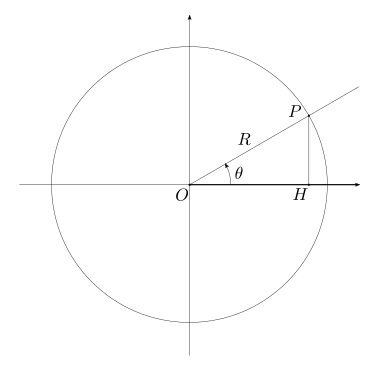
\includegraphics[width=.95\textwidth]{../../media/trigonometry-def.png}
\end{minipage}\\
\end{aligned}\end{align*}

\subsection{Relazione fondamentale della trignometria}
\label{\detokenize{ch/trigonometry:relazione-fondamentale-della-trignometria}}
\sphinxAtStartPar
Usando il teorema di Pitagora è immediato dimostrare la \sphinxstylestrong{relazione fondamentale della trigonometria} tra le funzioni seno e coseno di un angolo,
\begin{equation*}
\begin{split}\sin^2 \theta + \cos^2 \theta = 1 \ .\end{split}
\end{equation*}
\sphinxAtStartPar
\sphinxstylestrong{Nota sulla notazione.} Nell’uso delle funzioni trigonometriche, \(\sin^2 x\) indica il quadrato della funzione e non la composizione della funzione con se stessa,
\begin{equation*}
\begin{split}\sin^2 x = (\sin x)^2 \neq \sin( \sin x) \ .\end{split}
\end{equation*}

\subsection{Altre funzioni trigonometriche}
\label{\detokenize{ch/trigonometry:altre-funzioni-trigonometriche}}
\sphinxAtStartPar
\sphinxstylestrong{Tangente.} \(\tan \theta := \dfrac{\sin \theta}{\cos \theta} = \dfrac{\overline{PH}}{\overline{OH}} \ .\)

\sphinxAtStartPar
\sphinxstyleemphasis{Cosecante, secante, cotangente.} Definizioni al limite tra l’inutile e il dannoso,
\begin{equation*}
\begin{split}\begin{aligned}
  \text{cosec} \ \theta & := \frac{1}{\sin \theta} \\
  \text{sec  } \ \theta & := \frac{1}{\cos \theta} \\
  \text{cotan} \ \theta & := \frac{1}{\tan \theta} \\
\end{aligned}\end{split}
\end{equation*}

\section{Angoli particolari e proprietà}
\label{\detokenize{ch/trigonometry:angoli-particolari-e-proprieta}}\begin{equation*}
\begin{split}
\begin{minipage}[t]{.40\textwidth}
  \vspace{0pt}
  \textbf{Angoli particolari.}
  \begin{equation*}
  \begin{matrix}
   \theta & \cos \theta & \sin \theta & \tan \theta \\
   \hline 
   0             & 1                  & 0                  & 0                  \\
   \frac{\pi}{6} & \frac{\sqrt{3}}{2} & \frac{1}{2}        & \frac{1}{\sqrt{3}} \\
   \frac{\pi}{4} & \frac{\sqrt{2}}{2} & \frac{\sqrt{2}}{2} & 1                  \\
   \frac{\pi}{3} & \frac{1}{2}        & \frac{\sqrt{3}}{2} & \sqrt{3}           \\
   \frac{\pi}{2} & 0                  & 1                  & \rightarrow \infty \\
  \end{matrix}
  \end{equation*}
  \textbf{Proprietà.}
  \begin{equation*}
  \begin{aligned}
    \sin\left(-x\right)              & = - \sin x \\ 
    \cos\left(-x\right)              & =   \cos x \\ 
    \sin\left(x+\frac{\pi}{2}\right) & =   \cos x \\  
    \cos\left(x+\frac{\pi}{2}\right) & = - \sin x \\  
    \sin(x + \pi)                    & = - \sin x \\
    \cos(x + \pi)                    & = - \cos x \\
  \end{aligned}
  \end{equation*}
\end{minipage}
\hspace{.05\textwidth}
\begin{minipage}[t]{.55\textwidth}
  \vspace{0pt}
  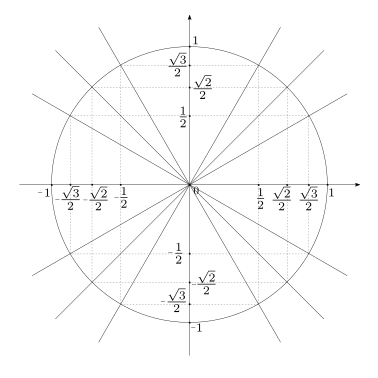
\includegraphics[width=.95\textwidth]{../../media/trigonometry-particular.png}
\end{minipage}
\end{split}
\end{equation*}

\section{Formule di somma e sottrazione}
\label{\detokenize{ch/trigonometry:formule-di-somma-e-sottrazione}}
\sphinxAtStartPar
Valgono le seguenti formule per il coseno e il seno della somma e della differenza di angoli,
\begin{equation*}
\begin{split}\begin{aligned}
  \cos ( x \mp y ) & = \cos x \ \cos y \pm \sin x \ \sin y \\
  \sin ( x \mp y ) & = \sin x \ \cos y \mp \cos x \ \sin y \\
\end{aligned}\end{split}
\end{equation*}
\sphinxAtStartPar
Per completezza, come utile esercizio di geometria sulla similitudine dei triangoli, e per familiarizzare con le funzioni armoniche, si fornisce la dimostrazione della formula del coseno della somma.
\subsubsection*{Dimostrazione di \protect\(\ \cos ( x + y ) = \cos x \ \cos y - \sin x \ \sin y\protect\)}

\begin{figure}[htbp]
\centering

\noindent\sphinxincludegraphics{{trigonometry-sum}.png}
\end{figure}

\sphinxAtStartPar
Partendo dall’interpretazione geometrica del coseno di \(\alpha + \beta\),
\begin{equation*}
\begin{split}\cos ( \alpha + \beta ) = \frac{\overline{OF}}{R}\end{split}
\end{equation*}
\sphinxAtStartPar
è necessario esprimere la lunghezza del segmento \(OF\) come multiplo del raggio \(R\).



\sphinxAtStartPar
Usando la similitudine dei triangoli \(OFE\), \(OCA\), e riconoscendo il coseno dell’angolo \(\alpha\),
\begin{equation*}
\begin{split}\overline{OF} = \frac{\overline{OC}}{\overline{OA}} \overline{OE} = \cos \alpha \ \overline{OE} \ .\end{split}
\end{equation*}
\sphinxAtStartPar
La lunghezza del segmento \(OE\) può essere scritta come differenza della lunghezza di \(OD\) e quella di \(ED\); queste ultime due lunghezze possono essere espresse come frazioni del raggio della circonferenza \(R = \overline{OB}\), grazie all’uso delle funzioni trigonometriche e alla similitudine dei triangoli (\(\overline{ED} = \sin \alpha \, \overline{BE} = \sin \alpha \, \frac{\overline{BD}}{\cos \alpha} = \sin \alpha \, \frac{\overline{OB} \sin \beta}{\cos \alpha}\)),
\begin{equation*}
\begin{split}\begin{aligned}
\overline{OE} = \overline{OD} - \overline{ED} & = \overline{OB} \cos \beta - \overline{OB} \sin \beta \frac{\sin \alpha}{\cos \alpha} = \\
& = R \left( \cos \beta - \overline{OB} \sin \beta \frac{\sin \alpha}{\cos \alpha} \right)
\end{aligned}\end{split}
\end{equation*}
\sphinxAtStartPar
Sostituendo questa espressione di \(\overline{OE}\) nell’espressione di \(\overline{OF}\), si ottiene
\begin{equation*}
\begin{split}\overline{OF} = \overline{OB} \left( \cos \alpha \cos \beta - \sin \beta \sin \alpha  \right)\end{split}
\end{equation*}
\sphinxAtStartPar
dalla quale si ottiene la relazione desiderata,
\begin{equation*}
\begin{split}\cos (\alpha + \beta) = \cos \alpha \cos \beta - \sin \beta \sin \alpha \ .\end{split}
\end{equation*}

\section{Werner}
\label{\detokenize{ch/trigonometry:werner}}\begin{equation*}
\begin{split}\begin{aligned}
  \cos x \cos y & = \dfrac{1}{2} \left[ \cos( x - y ) + \cos ( x + y ) \right] \\
  \sin x \sin y & = \dfrac{1}{2} \left[ \cos( x - y ) - \cos ( x + y ) \right] \\
  \sin x \cos y & = \dfrac{1}{2} \left[ \sin( x - y ) + \sin ( x + y ) \right] \\
\end{aligned}\end{split}
\end{equation*}\subsubsection*{Dimostrazione di \protect\(\ \cos x \cos y = \dfrac{1}{2} \left[ \cos( x - y ) + \cos ( x + y ) \right]\protect\)}

\sphinxAtStartPar
Usando le formule del coseno della somma e della sottrazione di una coppia di angoli,
\begin{equation*}
\begin{split}\begin{aligned}
  \cos( x - y ) & = \cos x \cos y + \sin x \sin y \\
  \cos( x + y ) & = \cos x \cos y - \sin x \sin y \\
\end{aligned}\end{split}
\end{equation*}
\sphinxAtStartPar
sommando termine a termine si ottiene
\begin{equation*}
\begin{split}\cos (x - y) + \cos( x + y ) = 2 \cos x \cos y \ ,\end{split}
\end{equation*}
\sphinxAtStartPar
dalla quale risulta evidente la relazione desiderata.


\section{Prostaferesi}
\label{\detokenize{ch/trigonometry:prostaferesi}}
\sphinxAtStartPar
Definendo \(p = x-y\) e \(q = x+y\) nelle formule di Werner, è immediato ricavare
\begin{equation*}
\begin{split}\begin{aligned}
  \cos p + \cos q & = 2 \cos\left(\frac{p+q}{2} \right) \cos\left(\frac{q-p}{2} \right) \\
  \cos p - \cos q & = 2 \sin\left(\frac{p+q}{2} \right) \sin\left(\frac{q-p}{2} \right) \\
  \sin p + \sin q & = 2 \sin\left(\frac{p+q}{2} \right) \cos\left(\frac{q-p}{2} \right) \\
\end{aligned}\end{split}
\end{equation*}\subsubsection*{Dimostrazione di \protect\(\ \cos p + \cos q = 2 \cos\left(\frac{p+q}{2} \right) \cos\left(\frac{q-p}{2} \right)\protect\)}

\sphinxAtStartPar
Usando la formula di Werner per il prodotto dei coseni,
\begin{equation*}
\begin{split}\cos x \cos y = \frac{1}{2} \left[ \cos(x-y) + \cos(x+y) \right]\end{split}
\end{equation*}
\sphinxAtStartPar
e definendo
\begin{equation*}
\begin{split}\begin{cases}
  x-y = p \\
  x+y = q \\
\end{cases}
\qquad \rightarrow \qquad
\begin{cases}
  2 x = p + q \\
  2 y = q - p \\
\end{cases}
\qquad \rightarrow \qquad
\begin{cases}
  x = \frac{ p + q }{2} \\
  y = \frac{ q - p }{2} \\
\end{cases}
\end{split}
\end{equation*}
\sphinxAtStartPar
si ottiene
\begin{equation*}
\begin{split}\cos \frac{p+q}{2} \cos\frac{q-p}{2} = \frac{1}{2} \left( \cos p + \cos q \right) \ ,\end{split}
\end{equation*}
\sphinxAtStartPar
dalla quale è evidente la relazione desiderata.

\sphinxstepscope


\chapter{Esponenziale e logaritmo}
\label{\detokenize{ch/precalculus/exponential_logarithm:esponenziale-e-logaritmo}}\label{\detokenize{ch/precalculus/exponential_logarithm:math-hs-exp-log}}\label{\detokenize{ch/precalculus/exponential_logarithm::doc}}
\sphinxAtStartPar
In questo capitolo si presentano le funzioni a variabile reale, \(f(x): D \in \mathbb{R} \rightarrow \mathbb{R}\):
\begin{itemize}
\item {} 
\sphinxAtStartPar
esponenziale, \(f(x) = a^x\)

\item {} 
\sphinxAtStartPar
logaritmo, \(f(x) = \log_a x\)

\end{itemize}

\sphinxAtStartPar
e successivamente le {\hyperref[\detokenize{ch/precalculus::doc}]{\sphinxcrossref{\DUrole{doc,std,std-doc}{funzioni iperboliche}}}}


\section{Funzione esponenziale e logaritmo di variabile reale}
\label{\detokenize{ch/precalculus/exponential_logarithm:funzione-esponenziale-e-logaritmo-di-variabile-reale}}

\subsection{Funzione esponenziale, \protect\(a^x\protect\)}
\label{\detokenize{ch/precalculus/exponential_logarithm:funzione-esponenziale-a-x}}\label{\detokenize{ch/precalculus/exponential_logarithm:math-hs-exp-ax-def}}
\sphinxAtStartPar
Nell’ambito dei numeri reali, l’elevamento alla potenza reale \(x \in \mathbb{R}\) di un numero reale \(a \in \mathbb{R}\),
\begin{equation*}
\begin{split}a^x\end{split}
\end{equation*}
\sphinxAtStartPar
è un’operazione ben definita per ogni valore dell’esponente \(x\) solo per base \(a \geq 0\). Per ogni valore di \(a \geq 0\) si può definire quindi la funzione esponenziale con base \(a\)
\begin{equation*}
\begin{split}f(x) = a^x \ ,\end{split}
\end{equation*}
\sphinxAtStartPar
che è definita per \(x \in \mathbb{R}\) e ha immagine \((0, +\infty)\).

\sphinxAtStartPar
\sphinxstylestrong{Proprietà.}
\begin{itemize}
\item {} 
\sphinxAtStartPar
la {\hyperref[\detokenize{ch/precalculus/real-functions:math-hs-precalculus-real-functions-types}]{\sphinxcrossref{\DUrole{std,std-ref}{funzione è monotona}}}}:
\begin{itemize}
\item {} 
\sphinxAtStartPar
se \(a > 1\), la funzione è monotona crescente

\item {} 
\sphinxAtStartPar
se \(a = 1\), la funzione è costante e uguale a \(1\)

\item {} 
\sphinxAtStartPar
se \(a < 1\), la funzione è monotona decrescente

\end{itemize}

\item {} 
\sphinxAtStartPar
la {\hyperref[\detokenize{ch/infinitesimal_calculus/analysis:infinitesimal-calculus-continuous-fun}]{\sphinxcrossref{\DUrole{std,std-ref}{funzione è continua}}}}, come si vedrà nel capitolo sull”{\hyperref[\detokenize{ch/infinitesimal_calculus/analysis:infinitesimal-calculus-analysis}]{\sphinxcrossref{\DUrole{std,std-ref}{introduzione all’analisi}}}}

\end{itemize}

\sphinxAtStartPar
Tra tutte le basi, la funzione esponenziale con base \(e\) di Eulero (o di Nepero) svolge un ruolo fondamentale in matematica e nelle scienze in generale, sia nell’ambito dei numeri reali sia nell’ambito dei numeri complessi, come ci sarà l’occasione di iniziare ad apprezzare nelle parti sul:
\begin{itemize}
\item {} 
\sphinxAtStartPar
{\hyperref[\detokenize{ch/calculus:math-hs-calculus}]{\sphinxcrossref{\DUrole{std,std-ref}{calcolo}}}}: {\hyperref[\detokenize{ch/infinitesimal_calculus/analysis:infinitesimal-calculus-limits}]{\sphinxcrossref{\DUrole{std,std-ref}{limiti}}}}, {\hyperref[\detokenize{ch/infinitesimal_calculus/derivatives:infinitesimal-calculus-derivatives}]{\sphinxcrossref{\DUrole{std,std-ref}{derivate}}}}, {\hyperref[\detokenize{ch/infinitesimal_calculus/integrals:infinitesimal-calculus-integrals}]{\sphinxcrossref{\DUrole{std,std-ref}{integrali}}}}, {\hyperref[\detokenize{ch/ode:ode-hs}]{\sphinxcrossref{\DUrole{std,std-ref}{equazioni differenziali}}}}

\item {} 
\sphinxAtStartPar
{\hyperref[\detokenize{ch/algebra/complex-algebra:math-hs-algebra-complex}]{\sphinxcrossref{\DUrole{std,std-ref}{numeri complessi}}}}

\end{itemize}

\sphinxAtStartPar
Vale dunque la pena introdurre la funzione esponenziale \(e^x\), e discuterne alcune definizioni equivalenti e proprietà fondamentali che permettono di comprendere l’origine della centralità di questa funzione in (quasi) tutti gli ambiti della matematica e delle scienze.

\sphinxAtStartPar
In questo capitolo ci si concentra sulla funzione esponenziale sul campo dei numeri reali, mentre si rimanda al capitolo sui {\hyperref[\detokenize{ch/algebra/complex-algebra:math-hs-algebra-complex}]{\sphinxcrossref{\DUrole{std,std-ref}{numeri complessi}}}} per la definizione dell’esponenziale complesso, e al capitolo sulle {\hyperref[\detokenize{ch/ode:ode-hs}]{\sphinxcrossref{\DUrole{std,std-ref}{equazioni differenziali ordinarie}}}} per le prime applicazioni fondamentali dell’esponenziale, con esponenti reali o complessi.


\subsection{Funzione esponenziale, \protect\(e^x\protect\)}
\label{\detokenize{ch/precalculus/exponential_logarithm:funzione-esponenziale-e-x}}\label{\detokenize{ch/precalculus/exponential_logarithm:math-hs-exp-def-ex}}
\sphinxAtStartPar
\sphinxstylestrong{Definizione.} Per ogni \(x \in \mathbb{R}\), è possibile dare diverse definizioni equivalenti della funzione esponenziale \(f(x) = e^x\), che può:
\begin{enumerate}
\sphinxsetlistlabels{\arabic}{enumi}{enumii}{}{.}%
\item {} 
\sphinxAtStartPar
essere intesa come l’elevamento a potenza della {\hyperref[\detokenize{ch/series:math-hs-series-e-euler}]{\sphinxcrossref{\DUrole{std,std-ref}{\(e\) di Eulero}}}} con la variabile indipendente \(x\) come esponente. Questa definizione «agnostica» considera \(e\) un numero con un determinato valore, approssimato \(2.718281828\text{e poi la magia finisce}\), tale da soddisfare le proprietà che si incontreranno nel percorso; queste proprietà sono diretta conseguenza e possono essere dimostrate grazie alle altre due definizioni equivalenti:

\item {} 
\sphinxAtStartPar
essere definita come limite della successione di funzioni \(\left( 1 + \frac{x}{n} \right)^n\)

\end{enumerate}
\begin{equation*}
\begin{split}
  e^x := \lim_{n \rightarrow \infty} \left( 1 + \frac{x}{n}\right)^n
\end{split}
\end{equation*}\begin{enumerate}
\sphinxsetlistlabels{\arabic}{enumi}{enumii}{}{.}%
\setcounter{enumi}{2}
\item {} 
\sphinxAtStartPar
essere definita come limite della serie di funzioni con elementi \(\frac{x^n}{n!}\),

\end{enumerate}
\begin{equation*}
\begin{split}
  e^x := \lim_{n \rightarrow \infty} \sum_{k=0}^{n} \frac{x^n}{n!} \\
\end{split}
\end{equation*}
\sphinxAtStartPar
Si può dimostrare che (seguire i link per le dimostrazioni in appendice):
\begin{itemize}
\item {} 
\sphinxAtStartPar
la {\hyperref[\detokenize{ch/precalculus/exponential_logarithm-notes:math-hs-exp-log-notes-convergence}]{\sphinxcrossref{\DUrole{std,std-ref}{serie è convergente}}}} per ogni \(x \in \mathbb{R}\) finito

\item {} 
\sphinxAtStartPar
le due {\hyperref[\detokenize{ch/precalculus/exponential_logarithm-notes:math-hs-exp-log-notes-equivalence}]{\sphinxcrossref{\DUrole{std,std-ref}{definizioni sono equivalenti}}}}

\item {} 
\sphinxAtStartPar
le definizioni della funzione \(e^x\) giustificano la notazione \(e^x\) questa funznione poiché soddisfa le {\hyperref[\detokenize{ch/precalculus/exponential_logarithm-notes:math-hs-exp-log-notes-powers}]{\sphinxcrossref{\DUrole{std,std-ref}{proprietà delle potenze (\sphinxstyleemphasis{con stessa base, \(e\)})}}}}:
\begin{equation*}
\begin{split}\begin{aligned}
    e^0 & = 1 \\
    e^1 & = e \\
    e^{x+y} & = e^x \, e^y \ .
  \end{aligned}\end{split}
\end{equation*}
\sphinxAtStartPar
Una conseguenza indiretta è l’equivalenza della definizione «agnostica» 1. e delle altre due.

\end{itemize}

\sphinxAtStartPar
Tra le conseguenze principali di questa definizione
\begin{itemize}
\item {} 
\sphinxAtStartPar
la derivata della funzione \(e^x\) è \(e^x\), ed è una delle {\hyperref[\detokenize{ch/infinitesimal_calculus/derivatives:infinitesimal-calculus-derivatives-fund}]{\sphinxcrossref{\DUrole{std,std-ref}{derivate fondamentali}}}} del {\hyperref[\detokenize{ch/infinitesimal_calculus/derivatives:infinitesimal-calculus-derivatives}]{\sphinxcrossref{\DUrole{std,std-ref}{calcolo differenziale}}}},
\begin{equation*}
\begin{split}\frac{d}{dx} e^x = e^x \ .\end{split}
\end{equation*}
\item {} 
\sphinxAtStartPar
l’integrale della funzione \(e^x\) è la stessa funzione
\begin{equation*}
\begin{split}\int e^x \, dx = e^x + C \ ,\end{split}
\end{equation*}
\sphinxAtStartPar
all’origine della battuta che non fa ridere \sphinxstylestrong{(!)} che spiega la tristezza della funzione \(e^x\) alla festa delle funzioni, con il fatto che la funzione \(e^x\) non si integra.

\end{itemize}




\subsection{Funzione logaritmo naturale, \protect\(\text{ln} \, x\protect\)}
\label{\detokenize{ch/precalculus/exponential_logarithm:funzione-logaritmo-naturale-text-ln-x}}\label{\detokenize{ch/precalculus/exponential_logarithm:math-hs-exp-def-ln}}
\sphinxAtStartPar
\sphinxstylestrong{Definizione.} Poiché la base \(e > 1\), la funzione \(e^x\) è monotona crescente, \(e^x: \mathbb{R} \rightarrow (0, +\infty)\), e quindi esiste la sua {\hyperref[\detokenize{ch/precalculus/real-functions:math-hs-precalculus-real-functions-inverse}]{\sphinxcrossref{\DUrole{std,std-ref}{funzione inversa}}}} con dominio \((0,+\infty)\) e immagine \(\mathbb{R}\). La funzione inversa della funzione esponenziale con base \(e\) viene definita \sphinxstylestrong{logaritmo naturale}, \(\ln x\). Cioè
\begin{equation*}
\begin{split}x = e^y \qquad \leftrightarrow \qquad y = \ln x\end{split}
\end{equation*}
\sphinxAtStartPar
o altrimenti, la definizione di logaritmo \(\ln ( e^x ) = x\), può essere reinterpretata come, \(f^{-1} \circ f(x) = x \), con
\begin{equation*}
\begin{split}f(x) = e^x \qquad \rightarrow \qquad f^{-1}(x) = \ln x \ .\end{split}
\end{equation*}

\subsection{Funzioni iperboliche}
\label{\detokenize{ch/precalculus/exponential_logarithm:funzioni-iperboliche}}\label{\detokenize{ch/precalculus/exponential_logarithm:math-hs-exp-def-hyp}}
\sphinxAtStartPar
Vengono definite le funzioni iperboliche
\begin{equation*}
\begin{split}\begin{aligned}
  \cosh x & := \frac{e^x + e^{-x}}{2} \\
  \sinh y & := \frac{e^x - e^{-x}}{2} \ 
\end{aligned}\end{split}
\end{equation*}
\sphinxAtStartPar
\sphinxstylestrong{Proprietà.}
Simmetria:
\begin{equation*}
\begin{split}\cosh(-x) = \cosh(x) \qquad , \qquad \sinh(-x) = - \sinh(x) \ .\end{split}
\end{equation*}
\sphinxAtStartPar
Le funzioni iperboliche hanno regole analoghe \sphinxhyphen{} ma non identiche \sphinxhyphen{} alle funzioni trigonometriche, {\hyperref[\detokenize{ch/precalculus/exponential_logarithm-notes:math-hs-exp-log-notes-hyp}]{\sphinxcrossref{\DUrole{std,std-ref}{dimostrabili}}}} grazie alle proprietà delle potenze
\begin{itemize}
\item {} 
\sphinxAtStartPar
Relazione fondamentale
\begin{equation*}
\begin{split}\cosh^2 x - \sinh^2 x = 1\end{split}
\end{equation*}
\item {} 
\sphinxAtStartPar
Somma e sottrazione
\begin{equation*}
\begin{split}\begin{aligned}
    \cosh(x \mp y) & = \cosh x \cosh y \mp \sinh x \sinh y \\
    \sinh(x \mp y) & = \sinh x \cosh y \mp \cosh x \sinh y 
  \end{aligned}\end{split}
\end{equation*}
\end{itemize}



\sphinxstepscope


\section{Problemi}
\label{\detokenize{ch/precalculus/exponential_logarithm-problems:problemi}}\label{\detokenize{ch/precalculus/exponential_logarithm-problems:math-hs-exp-log-problems}}\label{\detokenize{ch/precalculus/exponential_logarithm-problems::doc}}
\sphinxstepscope


\section{Soluzioni}
\label{\detokenize{ch/precalculus/exponential_logarithm-sol:soluzioni}}\label{\detokenize{ch/precalculus/exponential_logarithm-sol:math-hs-exp-log-sol}}\label{\detokenize{ch/precalculus/exponential_logarithm-sol::doc}}
\sphinxstepscope


\section{Note e dimostrazioni}
\label{\detokenize{ch/precalculus/exponential_logarithm-notes:note-e-dimostrazioni}}\label{\detokenize{ch/precalculus/exponential_logarithm-notes:math-hs-exp-log-notes}}\label{\detokenize{ch/precalculus/exponential_logarithm-notes::doc}}

\subsection{Funzione esponenziale}
\label{\detokenize{ch/precalculus/exponential_logarithm-notes:funzione-esponenziale}}\label{\detokenize{ch/precalculus/exponential_logarithm-notes:math-hs-exp-log-notes-exp}}

\subsubsection{Convergenza della serie di funzioni \protect\(\sum_{n=0}^{\infty} \frac{x^n}{n!}\protect\) in ogni intervallo limitato}
\label{\detokenize{ch/precalculus/exponential_logarithm-notes:convergenza-della-serie-di-funzioni-sum-n-0-infty-frac-x-n-n-in-ogni-intervallo-limitato}}\label{\detokenize{ch/precalculus/exponential_logarithm-notes:math-hs-exp-log-notes-convergence}}
\sphinxAtStartPar
Per dimostrare la convergenza uniforme di \(\sum_{k=0}^{\infty} \frac{x^k}{k!}\) a \(e^x\) in ogni intervallo limitato \(|x| < M\), è richiesto di dimostrare che per ogni \(\varepsilon > 0\) esiste \(N \in \mathbb{N}\) tale che
\begin{equation*}
\begin{split}|e^x - S_n(x)| < \varepsilon \ , \qquad \forall |x| < M \end{split}
\end{equation*}
\sphinxAtStartPar
per tutti gli \(n > N\). Bisogna quindi dimostrare che
\begin{equation*}
\begin{split}\left| \sum_{k=n+1}^{\infty} \frac{x^k}{k!} \right| < \varepsilon \ .\end{split}
\end{equation*}
\sphinxAtStartPar
Definendo \(\tilde{M} = \max\{ 1, M \}\)
\begin{equation*}
\begin{split}\left| \sum_{k=n+1}^{\infty} \frac{x^k}{k!} \right| < \sum_{k=n+1}^{\infty} \frac{\tilde{M}^k}{k!}\end{split}
\end{equation*}
\sphinxAtStartPar
e scegliendo \(k > 2 \tilde{M}\), in maniera da poter scrivere
\begin{equation*}
\begin{split}\frac{\tilde{M}^k}{k!} = \frac{\tilde{M}^{2 \tilde{M}}}{( 2 \tilde{M})!} \frac{\tilde{M}}{2\tilde{M}+1} \dots \frac{\tilde{M}}{k} <  \frac{\tilde{M}^{2 \tilde{M}}}{( 2 \tilde{M})!} 2^{-(k - \tilde{M})} = \frac{(2 \tilde{M})^{2 \tilde{M}}}{(2 \tilde{M})!} 2^{-k}\end{split}
\end{equation*}
\sphinxAtStartPar
e quindi
\begin{equation*}
\begin{split}\sum_{k=n+1}^{\infty} \frac{\tilde{M}}{k!} < \sum_{k=n+1}^{\infty} \frac{(2 \tilde{M})^{2 \tilde{M}}}{(2\tilde{M})!} 2^{-k} =  \frac{(2 \tilde{M})^{2 \tilde{M}}}{(2\tilde{M})!} 2^{-n}\end{split}
\end{equation*}
\sphinxAtStartPar
avendo usato \(\sum_{k=n+1}^{\infty} 2^{-k} = 2^{-n-1} \sum_{k=0}^{\infty} 2^{-k} = 2^{-n-1} \cdot 2 = 2^{-n}\).

\sphinxAtStartPar
Scegliendo \(N > \log_2 \left( \frac{1}{\varepsilon} \frac{(2\tilde{M})^{2 \tilde{M}}}{(2 \tilde{M})!)} \right)\), per ogni \(n > N\) si ha
\begin{equation*}
\begin{split}\left| \sum_{k=n+1}^{\infty} \frac{x^k}{k!} \right| <  \frac{(2 \tilde{M})^{2 \tilde{M}}}{(2\tilde{M})!} 2^{-n} <  \frac{(2 \tilde{M})^{2 \tilde{M}}}{(2\tilde{M})!} 2^{-N} < \varepsilon \ .\end{split}
\end{equation*}

\subsubsection{Equivalenza delle due definizioni}
\label{\detokenize{ch/precalculus/exponential_logarithm-notes:equivalenza-delle-due-definizioni}}\label{\detokenize{ch/precalculus/exponential_logarithm-notes:math-hs-exp-log-notes-equivalence}}

\subsubsection{Giustificazione della notazione \protect\(\ e^x\protect\)}
\label{\detokenize{ch/precalculus/exponential_logarithm-notes:giustificazione-della-notazione-e-x}}\label{\detokenize{ch/precalculus/exponential_logarithm-notes:math-hs-exp-log-notes-powers}}
\sphinxAtStartPar
Per evitare la forma indeterminata nel termine \(0^0\), si calcola qui il limite per \(x \rightarrow 0\) (\sphinxstylestrong{todo} \sphinxstyleemphasis{motivare la validità di questa operazione/interpretazione della funzione \(e^x\)})
\begin{equation*}
\begin{split}e^0 := \lim_{x \rightarrow 0} e^x = \lim_{x \rightarrow 0} \sum_{n = 0}^{\infty} \frac{x^n}{n!} = 1 + \lim_{x \rightarrow 0} \sum_{n=1}^{\infty} \frac{x^n}{n!} = 1 \ .\end{split}
\end{equation*}
\sphinxAtStartPar
Ricordando la definizione della {\hyperref[\detokenize{ch/series:math-hs-series-e-euler}]{\sphinxcrossref{\DUrole{std,std-ref}{\(e\) di Eulero}}}}, è immediato verificare che il valore della serie di funzioni per \(x = 1\) coincide con il valore di \(e\)
\begin{equation*}
\begin{split}e^1 = \sum_{n=0}^{\infty} \frac{x^n}{n!} \bigg|_{x=1} = \sum_{n=0}^{\infty} \frac{1}{n!} = e \ .\end{split}
\end{equation*}
\sphinxAtStartPar
La serie che definisce la esponenziale soddisfa la proprietà delle potenze \(e^x \, e^y = e^{x+y}\),
\begin{equation*}
\begin{split}\begin{aligned}
  e^x \, e^y 
  & = \sum_{n=0}^{\infty} \frac{x^n}{n!} \sum_{m = 0}^{\infty} \frac{y^m}{m!} = \\
  & = \sum_{n=0}^{\infty} \sum_{m=0}^{\infty} \frac{y^m}{m!} \frac{x^n}{n!} =  & \text{($m,n \  \rightarrow \ m,p=m+n$)}\\
  & = \sum_{p=0}^{\infty} \sum_{m=0}^{p} \frac{y^m \, x^{p-m}}{m! (p-m!)} = \\
  & = \sum_{p=0}^{\infty} \frac{1}{p!} \underbrace{\sum_{m=0}^{p} \frac{p!}{m! (p-m)!} y^m \, x^{p-m}}_{(x+y)^p} = \\
  & = \sum_{p=0}^{\infty} \frac{(x+y)^p}{p!} = \\
  & = e^{x+y} \ ,
\end{aligned}\end{split}
\end{equation*}
\sphinxAtStartPar
avendo usato il {\hyperref[\detokenize{ch/precalculus/polynomials:math-hs-precalculus-polynomials-binomial-thm}]{\sphinxcrossref{\DUrole{std,std-ref}{teorema binomiale}}}}.


\subsection{Funzioni iperboliche}
\label{\detokenize{ch/precalculus/exponential_logarithm-notes:funzioni-iperboliche}}\label{\detokenize{ch/precalculus/exponential_logarithm-notes:math-hs-exp-log-notes-hyp}}\subsubsection*{Relazione fondamentale}
\begin{equation*}
\begin{split}\cosh^2 x - \sinh^2 x = 1\end{split}
\end{equation*}
\sphinxAtStartPar
infatti
\begin{equation*}
\begin{split}\begin{aligned}
\cosh^2 x - \sinh^2 x & = \left(\frac{e^x + e^{-x}}{2}\right) - \left(\frac{e^x - e^{-x}}{2}\right) = \\
& = \frac{e^{2x} + 2 + e^{-2x} - \left( e^{2x} - 2 + e^{-2x}\right)}{4} = 1 \\
\end{aligned}\end{split}
\end{equation*}\subsubsection*{Prodotti}
\begin{equation*}
\begin{split}\cosh x \cosh y = \frac{e^x+e^{-x}}{2} \frac{e^y+e^{-y}}{2} = \frac{e^{x+y} + e^{x-y} + e^{-x+y} + e^{-x-y}}{4}\end{split}
\end{equation*}\begin{equation*}
\begin{split}\sinh x \sinh y = \frac{e^x-e^{-x}}{2} \frac{e^y-e^{-y}}{2} = \frac{e^{x+y} - e^{x-y} - e^{-x+y} + e^{-x-y}}{4}\end{split}
\end{equation*}\begin{equation*}
\begin{split}\sinh x \cosh y = \frac{e^x-e^{-x}}{2} \frac{e^y+e^{-y}}{2} = \frac{e^{x+y} + e^{x-y} - e^{-x+y} - e^{-x-y}}{4}\end{split}
\end{equation*}\subsubsection*{Somma e differenza}
\begin{equation*}
\begin{split}\begin{aligned}
  \cosh(x+y) & = \frac{e^{x+y} + e^{-x-y}}{2} = \\
   & = \cosh x \cosh y + \sinh x \sinh y
\end{aligned}\end{split}
\end{equation*}\begin{equation*}
\begin{split}\begin{aligned}
  \cosh(x-y) & = \frac{e^{x-y} + e^{-x+y}}{2} = \\
   & = \cosh x \cosh y - \sinh x \sinh y
\end{aligned}\end{split}
\end{equation*}\begin{equation*}
\begin{split}\begin{aligned}
  \sinh(x+y) & = \frac{e^{x+y} - e^{-x-y}}{2} = \\
   & = \sinh x \cosh y + \cosh x \sinh y
\end{aligned}\end{split}
\end{equation*}\begin{equation*}
\begin{split}\begin{aligned}
  \sinh(x-y) & = \frac{e^{x-y} - e^{-x+y}}{2} = \\
   & = \sinh x \cosh y - \cosh x \sinh y
\end{aligned}\end{split}
\end{equation*}\subsubsection*{…}

\sphinxstepscope




\chapter{Algebra complessa}
\label{\detokenize{ch/algebra/complex-algebra:algebra-complessa}}\label{\detokenize{ch/algebra/complex-algebra:math-hs-algebra-complex}}\label{\detokenize{ch/algebra/complex-algebra::doc}}
\sphinxAtStartPar
Esistono collegamenti a questo capitolo da:
\begin{itemize}
\item {} 
\sphinxAtStartPar
la sezione sui {\hyperref[\detokenize{ch/set/numeric-sets:sets-numeric-c}]{\sphinxcrossref{\DUrole{std,std-ref}{numeri complessi}}}} nel capitolo sugli {\hyperref[\detokenize{ch/set/numeric-sets:sets-numeric}]{\sphinxcrossref{\DUrole{std,std-ref}{insiemi numerici}}}}

\item {} 
\sphinxAtStartPar
la sezione sull”{\hyperref[\detokenize{ch/algebra/complex-algebra-link:math-hs-algebra-complex-link}]{\sphinxcrossref{\DUrole{std,std-ref}{algebra sui numeri complessi}}}} nel capitolo sull”{\hyperref[\detokenize{ch/algebra:math-hs-algebra}]{\sphinxcrossref{\DUrole{std,std-ref}{algebra}}}}

\end{itemize}

\sphinxAtStartPar
In questa sezione viene introdotto l’insieme dei numeri complessi e le operazioni su di essi che permettono di definire l’algebra complessa.

\sphinxAtStartPar
I numeri reali sono sottoinsieme dei numeri complessi, \(\mathbb{R} \subset \mathbb{C}\). La definizione di operazioni e funzioni, come l’esponenziale, sui numeri complessi viene data come \sphinxstylestrong{estensione ai numeri complessi} delle definizioni note sui numeri reali.

\sphinxAtStartPar
I numeri complessi risultano utili in molti ambiti della matematica e della scienza, dalla fisica all’ingegneria:
\begin{itemize}
\item {} 
\sphinxAtStartPar
teorema fondamentale dell’algebra

\item {} 
\sphinxAtStartPar
rappresentazione efficace delle funzioni trigonometriche, grazie all’identità di Eulero

\item {} 
\sphinxAtStartPar
soluzione di equazioni differenziali

\item {} 
\sphinxAtStartPar
…

\end{itemize}




\section{Definizioni}
\label{\detokenize{ch/algebra/complex-algebra:definizioni}}\label{\detokenize{ch/algebra/complex-algebra:math-hs-algebra-complex-def}}
\sphinxAtStartPar
I numeri complessi estendono il campo dei numeri reali, \(\mathbb{R} \subset \mathbb{C}\). Viene inizialmente definita l”\sphinxstylestrong{unità immaginaria}, \(i\), come la radice quadra di \(-1\),
\begin{equation*}
\begin{split}i := \sqrt{-1} \ ,\end{split}
\end{equation*}
\sphinxAtStartPar
\sphinxstylestrong{todo} \sphinxstyleemphasis{discutere la definizione, facendo riferimento alle} \sphinxstylestrong{potenze}
\label{ch/algebra/complex-algebra:definition-0}
\begin{sphinxadmonition}{note}{Definition 20.1.1 (Numeri complessi \sphinxhyphen{} rappresentazione cartesiana)}



\sphinxAtStartPar
L’insieme dei numeri complessi, indicato con \(\mathbb{C}\), è l’insieme di quei numeri che possono essere scritti come
\begin{equation*}
\begin{split}z = x + i y \ ,\end{split}
\end{equation*}
\sphinxAtStartPar
con \(x, \ y \in \mathbb{R}\).
\end{sphinxadmonition}


\section{Operazioni con i numeri complessi \sphinxhyphen{} in forma cartesiana}
\label{\detokenize{ch/algebra/complex-algebra:operazioni-con-i-numeri-complessi-in-forma-cartesiana}}\label{\detokenize{ch/algebra/complex-algebra:math-hs-algebra-complex-operations-0}}\begin{itemize}
\item {} 
\sphinxAtStartPar
somma: \(z_1 + z_2 = (x_1 + i y_1) + (x_2 + i y_2) = (x_1 + x_2) + i (y_1 + y_2)\)

\item {} 
\sphinxAtStartPar
prodotto: \(z_1 z_2 = (x_1 + i y_1)(x_2 + i y_2) = x_1 x_2 - y_1 y_2 + i (x_1 y_2 + x_2 y_1)\)

\item {} 
\sphinxAtStartPar
potenza con esponente naturale, \(n \in \mathbb{N}\): \(z^n = (x + i y)^n = \underbrace{(x+iy) \dots (x+iy)}_{n \text{ volte}}\)

\item {} 
\sphinxAtStartPar
complesso coniugato: \(z^* := (x+iy)^* = x - i y\)

\item {} 
\sphinxAtStartPar
modulo: \(|z| := \sqrt{z^* z} = \sqrt{x^2 + y^2}\)

\end{itemize}


\section{Formula di de Moivre, esponenziale complesso e formula di Eulero}
\label{\detokenize{ch/algebra/complex-algebra:formula-di-de-moivre-esponenziale-complesso-e-formula-di-eulero}}\label{\detokenize{ch/algebra/complex-algebra:math-hs-algebra-complex-demoivre-euler}}
\sphinxAtStartPar
La formula di \sphinxstylestrong{de Moivre} è la relazione
\begin{equation}\label{equation:ch/algebra/complex-algebra:complex:demoivre}
\begin{split}(\cos x + i \sin x)^n = \cos(nx) + i \sin(nx) \ , \quad n \in \mathbb{Z} \ ,\end{split}
\end{equation}
\sphinxAtStartPar
per \(x \in \mathbb{R}\) e \(n \in \mathbb{Z}\). In appendice la {\hyperref[\detokenize{ch/algebra/complex-algebra-notes:math-hs-algebra-complex-notes-demoivre}]{\sphinxcrossref{\DUrole{std,std-ref}{dimostrazione della formula di de Moivre}}}}.

\sphinxAtStartPar
L”\sphinxstylestrong{esponenziale di un numero complesso}, \(z \in \mathbb{C}\), è definito estendendo la definizione di esponenziale per i numeri reali ai numeri complessi
\begin{equation}\label{equation:ch/algebra/complex-algebra:complex:complex-exp}
\begin{split}e^z = \sum_{n = 0}^{+\infty} \frac{z^n}{n!} = \lim_{n \rightarrow +\infty} \left( 1 + \frac{z}{n} \right)^n\end{split}
\end{equation}
\sphinxAtStartPar
Data questa definizione di esponenziale complesso, si può dimostrare la \sphinxstylestrong{formula di Eulero}
\begin{equation}\label{equation:ch/algebra/complex-algebra:complex:euler}
\begin{split}e^{i \theta} = \cos \theta + i \sin \theta \ ,\end{split}
\end{equation}
\sphinxAtStartPar
con \(\theta \in \mathbb{R}\). Vengono riportate in appendice due {\hyperref[\detokenize{ch/algebra/complex-algebra-notes:math-hs-algebra-complex-notes-euler}]{\sphinxcrossref{\DUrole{std,std-ref}{dimostrazioni della formula di Eulero}}}}, una usando la definizione di esponenziale complesso e la formula di de Moivre, l’altra usando le serie di Taylor.

\sphinxAtStartPar
Grazie alla formula di Eulero e alle proprietà elementari delle funzioni trigonometriche, \(\cos(-\theta) = \cos \theta\), \(\sin(-\theta) = -\sin \theta\), con \(\theta \in \mathbb{R}\), segue
\begin{equation}\label{equation:ch/algebra/complex-algebra:complex:cos-sin}
\begin{split}\begin{aligned}
 \cos \theta & = \frac{e^{i\theta} + e^{-i\theta}}{2} \\
 \sin \theta & = \frac{e^{i\theta} - e^{-i\theta}}{2i} \\
\end{aligned}\end{split}
\end{equation}

\section{Rappresentazione dei numeri complessi nel piano complesso (Argand\sphinxhyphen{}Gauss)}
\label{\detokenize{ch/algebra/complex-algebra:rappresentazione-dei-numeri-complessi-nel-piano-complesso-argand-gauss}}\label{\detokenize{ch/algebra/complex-algebra:math-hs-algebra-complex-complex-plane}}
\sphinxAtStartPar
Ogni numero complesso \(z \subset \mathbb{C}\) può essere associato a un punto del piano complesso \(\mathbb{C}\); l’uso di coordinate cartesiane o polari per la descrizione dei punti del piano \(\mathbb{R}^2\) suggerisce due tipi di rappresentazioni per un numero complesso:
\begin{itemize}
\item {} 
\sphinxAtStartPar
la \sphinxstylestrong{rappresentazione cartesiana} associa l’asse delle ascisse alla parte reale \(x\) e l’asse delle ordinate alla parte immaginaria \(y\),
\begin{equation*}
\begin{split}z = x + i y\end{split}
\end{equation*}
\item {} 
\sphinxAtStartPar
la \sphinxstylestrong{rappresentazione polare}; usando la legge di trasformazione tra coordinate polari \((r, \theta)\) e coordinate cartesiante \((x,y)\)
\begin{equation*}
\begin{split}\begin{cases}
    x = r \cos \theta \\
    y = r \sin \theta
  \end{cases}\end{split}
\end{equation*}
\sphinxAtStartPar
e la {\hyperref[\detokenize{ch/algebra/complex-algebra-notes:math-hs-algebra-complex-notes-euler}]{\sphinxcrossref{\DUrole{std,std-ref}{formula di Eulero}}}}, \(e^{i \theta} = \cos \theta + i \sin \theta\), è possibile scrivere un numero complesso in forma polare,
\begin{equation*}
\begin{split}z = x + i y = r \cos \theta + i r \sin \theta = r \left( \cos \theta + i \sin \theta \right) = r e^{i \theta} \ .\end{split}
\end{equation*}
\end{itemize}

\begin{sphinxadmonition}{note}{Nota:}
\sphinxAtStartPar
Le due rappresentazioni non sono equivalenti. Mentre la rappresentazione cartesiana permette di creare una relazione biunivoca tra i numeri complessi \(z = x + i \, y\) e i punti nel piano \((x, \ y)\), la rappresentazione polare assegna infiniti numeri complessi, seppur di uguale valore \(r \, e^{i \theta} = r \, e^{i (\theta + n \, 2 \pi)}\), con \(n \in \mathbb{Z}\) allo stesso punto nello spazio.
\end{sphinxadmonition}


\section{Operazioni con i numeri complessi}
\label{\detokenize{ch/algebra/complex-algebra:operazioni-con-i-numeri-complessi}}\label{\detokenize{ch/algebra/complex-algebra:math-hs-algebra-complex-operations}}
\sphinxAtStartPar
Si rivisitano ora le operazioni già presentate, mostrando la convenienza della rappresentazione polare per prodotti e potenze.


\subsection{Somma e prodotto}
\label{\detokenize{ch/algebra/complex-algebra:somma-e-prodotto}}
\sphinxAtStartPar
\sphinxstylestrong{Somma.} La somma di due numeri complessi è il numero complesso
\begin{equation*}
\begin{split}z_1 + z_2 = (x_1 + x_2) + i(y_1 + y_2)\end{split}
\end{equation*}
\sphinxAtStartPar
\sphinxstylestrong{Prodotto.} Il prodotto tra due numeri complessi \(z_1 = x_1 + i y_1 = r_1 e^{i \theta_1}\), \(z_2 = x_2 + i y_2 = r_2 e^{i \theta_2}\), è il numero complesso \(z_1 \cdot z_2 \in \mathbb{C}\) che può essere calcolato usando la proprietà distributiva tra somma e prodotto e la proprietà degli esponenti,
\begin{equation*}
\begin{split}\begin{aligned}
    z_1 \, z_2 
    & = r_1 \, r_2 e^{i(\theta_1 + \theta_2)} = \\
    & = (x_1 + i y_1 ) (x_2 + i y_2) = (x_1 x_2 - y_1 y_2)+i(x_1 y_2 + y_1 x_2) \\
  \end{aligned}\end{split}
\end{equation*}

\subsection{Complesso coniugato e modulo}
\label{\detokenize{ch/algebra/complex-algebra:complesso-coniugato-e-modulo}}
\sphinxAtStartPar
\sphinxstylestrong{Complesso coniugato.} Il complesso coniugato \(z^*\) di un numero compless \(z \in \mathbb{C}\) è il numero complesso con stessa parte reale e parte immaginaria opposta. Analogamente ha stesso modulo e argomento (definito tra \(-\pi\) e \(\pi\)) opposto
\begin{equation*}
\begin{split}z^* := x - i y = r e^{-i\theta} \end{split}
\end{equation*}
\sphinxAtStartPar
E” immediato {\hyperref[\detokenize{ch/algebra/complex-algebra-problems:math-hs-algebra-complex-problems-operations-cc-re-im}]{\sphinxcrossref{\DUrole{std,std-ref}{verificare}}}} le seguenti identità
\begin{equation}\label{equation:ch/algebra/complex-algebra:complex:cc:re-im}
\begin{split}\begin{aligned}
  \text{re}\{ z \} & = x = \frac{z + z^*}{2} \\
  \text{im}\{ z \} & = y = \frac{z - z^*}{2i} \\
\end{aligned}\end{split}
\end{equation}
\sphinxAtStartPar
\sphinxstylestrong{Valore assoluto.} Il valore assoluto di un numero complesso è uguale a
\begin{equation*}
\begin{split}\begin{aligned}
    |z| & := \sqrt{z^* z} = \\
    & = \sqrt{(x-iy)(x+iy)} =  \sqrt{x^2 + y^2} = \\
    & = \sqrt{r e^{-i\theta} r e^{i\theta}} = r
  \end{aligned}\end{split}
\end{equation*}

\subsection{Potenze e radici}
\label{\detokenize{ch/algebra/complex-algebra:potenze-e-radici}}
\sphinxAtStartPar
\sphinxstylestrong{Potenza.} Si presenta l’elevamento a potenza di un numero complesso,
\begin{equation*}
\begin{split}z = A e^{i (\alpha + 2 \pi n)} \ , \quad n \in \mathbb{Z} \ ,\end{split}
\end{equation*}
\sphinxAtStartPar
ricordando l’arbitrarietà nella rappresentazione in forma polare. Si rimanda all’appendice per il caso generale, mentre qui si presentano i casi con:


\subsubsection{Potenza intera, \protect\(p \in \mathbb{Z}\protect\).}
\label{\detokenize{ch/algebra/complex-algebra:potenza-intera-p-in-mathbb-z}}\begin{equation*}
\begin{split}z^p = A^p e^{i ( p \alpha + 2 \pi n p )} = A^{p} e^{i ( p \alpha + 2 \pi m )} \ , \quad m \in \mathbb{Z}\end{split}
\end{equation*}

\subsubsection{Radici o potenza \protect\(\frac{1}{p}, \ p \in \mathbb{Z}\protect\)}
\label{\detokenize{ch/algebra/complex-algebra:radici-o-potenza-frac-1-p-p-in-mathbb-z}}
\sphinxAtStartPar
La radice \(p\)\sphinxhyphen{}esima intera, \(p \in \mathbb{Z}\), di un numero complesso può essere interpretata come la potenza con esponente \(\frac{1}{p}, \ p \in \mathbb{Z}\),
\begin{equation*}
\begin{split}z^{\frac{1}{p}} = \left( r e^{i ( \theta + n 2 \pi ) } \right)^\frac{1}{p} = r^{\frac{1}{p}} e^{i \left(\frac{\theta}{p} + 2 \pi \frac{n}{p} \right)} \ , \quad n = \{ 0, 1, \dots, p-1\}\end{split}
\end{equation*}
\sphinxAtStartPar
e quindi corrisponde ai \(p\) numeri complessi con modulo \(r^{\frac{1}{p}}\) e argomenti \(\frac{\theta}{p} + 2 \pi \frac{n}{p}\).


\subsubsection{Potenza razionale}
\label{\detokenize{ch/algebra/complex-algebra:potenza-razionale}}
\sphinxAtStartPar
La potenza con esponente razionale, \(p, q \in \mathbb{Z}\), \(q \ne 0\), \(\frac{p}{q} = r + \frac{p'}{q}\), con \(p' < q\) e \(\frac{p'}{q}\) irriducibile, è ben definita per ogni numero complesso a differenza di quanto accade sui numeri reali.
\begin{equation*}
\begin{split}z^{\frac{p}{q}} = A^{\frac{p}{q}} e^{i \frac{p}{q} (\alpha + 2 \pi n)} = A^{\frac{p}{q}} e^{i (\frac{p}{q} \alpha + \frac{p'}{q} 2 \pi n)}\end{split}
\end{equation*}
\sphinxAtStartPar
Esistono quindi \(q\) risultati distinti per \(n \in \{ 0, 1, 2, \dots, q-1 \}\).


\subsection{Altre operazioni}
\label{\detokenize{ch/algebra/complex-algebra:altre-operazioni}}
\sphinxAtStartPar
\sphinxstylestrong{Potenza con esponente irrazinoale.} La potenza di un numero complesso \(z^p\) con esponente reale irrazionale \(p \in \mathbb{R} \backslash \mathbb{Q}\) produce gli infiniti numeri complessi con modulo \(r^p\) e \sphinxstyleemphasis{argomento \(p \theta + 2 \pi n p\) qualsiasi, per \(n \in \mathbb{Z}\)}

\sphinxAtStartPar
\sphinxstylestrong{Potenza qualsiasi.} Per la discussione di una {\hyperref[\detokenize{ch/algebra/complex-algebra-notes:math-hs-algebra-complex-notes-fun-power}]{\sphinxcrossref{\DUrole{std,std-ref}{potenza qualsiasi}}}} di un numero complesso si rimanda alla sezione sulle funzioni di variabile complessa in appendice.

\sphinxAtStartPar
\sphinxstylestrong{Esponenziale.} Per la discussione dell”{\hyperref[\detokenize{ch/algebra/complex-algebra-notes:math-hs-algebra-complex-notes-fun-exp}]{\sphinxcrossref{\DUrole{std,std-ref}{esponenziale complesso}}}} si rimanda alla sezione sulle funzioni di variabile complessa in appendice.

\sphinxAtStartPar
\sphinxstylestrong{Logaritmo.} Per la discussione del {\hyperref[\detokenize{ch/algebra/complex-algebra-notes:math-hs-algebra-complex-notes-fun-log}]{\sphinxcrossref{\DUrole{std,std-ref}{logaritmo complesso}}}} si rimanda alla sezione sulle funzioni di variabile complessa in appendice.


\section{Teorema fondamentale dell’algebra}
\label{\detokenize{ch/algebra/complex-algebra:teorema-fondamentale-dell-algebra}}\label{\detokenize{ch/algebra/complex-algebra:math-hs-algebra-complex-fund-thm}}
\sphinxAtStartPar
Ogni polinomio a coefficienti reali (\sphinxstylestrong{todo} o anche complessi) di grado \(n\), \(p_n(x) = a_n x^n + a_{n-1} x^{n-1} + \dots a_1 x + a_0\) può essere fattorizzato come prodotto di \(n\) binomi
\begin{equation*}
\begin{split}p_n(x) = a_n ( x - z_1 )( x - z_2 )\dots( x - z_n) \ ,\end{split}
\end{equation*}
\sphinxAtStartPar
e i numeri \(z_k \in \mathbb{C}\), \(k = 1:n\), sono chiamati \sphinxstylestrong{zeri} del polinomio.

\sphinxAtStartPar
Come diretta conseguenza, ogni equazione polinomiale di grado \(n\), \(p_n(x) = 0\), ammette \(n\) soluzioni complesse coincidenti con gli zeri \(z_k\) del polinomio \(p_n(x)\).


\section{Numeri complessi e geometria nel piano euclideo}
\label{\detokenize{ch/algebra/complex-algebra:numeri-complessi-e-geometria-nel-piano-euclideo}}\label{\detokenize{ch/algebra/complex-algebra:math-hs-algebra-complex-geometry-2d}}
\sphinxAtStartPar
La {\hyperref[\detokenize{ch/algebra::doc}]{\sphinxcrossref{\DUrole{doc,std,std-doc}{rappresentazione cartesiana}}}} dei numeri complessi \(z = x + i y\) crea un legame biunivoco tra i numeri complessi e i punti di un piano. Quindi è possibile affrontare la geometria analitica nel piano usando i numeri complessi:


\subsection{Posizione di un punto nel piano}
\label{\detokenize{ch/algebra/complex-algebra:posizione-di-un-punto-nel-piano}}
\sphinxAtStartPar
Una volta scelto un sistema di coordinate regolari, la posizione di un punto \(P\) nel piano è identificata dai valori delle sue coordinate. Utilizzando un sistema di coordinate cartsiane o polari il punto \(P\) è identificato dalle coppie di valori \(x_P, y_P\) o \(r_P, \theta_P\) rispettivamente. Associando l’asse \(x\) all’asse dei numeri reali e l’asse \(y\) all’asse dei numeri immaginari, si può associare il punto \(P \equiv (x_P, y_P)\) in maniera biunivoca al numero complesso \(z_P = x_P + i y_P\), mentre alle coordinate polari corrisponde la rappresentazione polare,
\begin{equation*}
\begin{split}z_P = x_P + i y_P = r e^{i \theta} \ .\end{split}
\end{equation*}

\subsection{Distanza tra punti}
\label{\detokenize{ch/algebra/complex-algebra:distanza-tra-punti}}
\sphinxAtStartPar
La distanza tra due punti nel piano può essere facilmente calcolata usando le coordiante cartesiane dei punti, tramite il teorema di Pitagora,
\begin{equation*}
\begin{split}|P_2 - P_1|^2 = (x_2 - x_1)^2 + (y_2 - y_1)^2 \ ,\end{split}
\end{equation*}
\sphinxAtStartPar
ed equivale al valore del numero complesso \(z_2 - z_1\),
\begin{equation*}
\begin{split}|z_2 - z_1|^2 = ((x_2-x_1) + i(y_2-y_1))^*((x_2-x_1) + i(y_2-y_1)) = (x_2 - x_1)^2 + (y_2 - y_1)^2 \end{split}
\end{equation*}

\subsection{Curva nel piano}
\label{\detokenize{ch/algebra/complex-algebra:curva-nel-piano}}
\sphinxAtStartPar
Una curva nel piano può essere rappresentata in forma esplicita, implicita o parametrica. Usando i numeri complessi,
\begin{itemize}
\item {} 
\sphinxAtStartPar
la forma implicita dell’equazione di una curva è una relazione della forma \(F(z)=0\), \(F_c(x, y) = 0\) o \(F_p(r, \theta) = 0\), ossia una funzione che lega i due parametri che definiscono un numero complesso, come per esempio parte reale e immaginaria o modulo e argomento; in alcuni casi, è possibile esprimere uno di questi parametri in funzione dell’altro nella forma esplicita

\item {} 
\sphinxAtStartPar
la forma parametrica dell’equazione di una curva può essere espressa come un numero complesso funzione di un parametro, come ad esempio
\begin{equation*}
\begin{split}z(s) = x(s) + i y(s) =  r(s) e^{i \theta(s)} \ .\end{split}
\end{equation*}
\sphinxAtStartPar
Questo equivale a fornire l’espressione parametrica della curva in termini delle coordinate cartesiane o polari.

\end{itemize}


\subsection{Intersezioni di curve}
\label{\detokenize{ch/algebra/complex-algebra:intersezioni-di-curve}}
\sphinxAtStartPar
Date due curve espresse in forma parametrica, \(\gamma_1: z_1(s)\), \(\gamma_2: z_2(r)\), gli eventuali punti di intersezione soddisfano la condizione \(z_1(\bar{s}) = z_2(\bar{r})\), cioè si ricerca il valore dei parametri \(s\), \(r\) per i quali i punti delle curve hanno le stesse coordinate.

\sphinxAtStartPar
Se le curve sono espresse in forma implicita, \(\gamma_1: F_1(z) = 0\), \(\gamma_2: F_2(z) = 0\), il problema della ricerca delle intersezioni si riduce alla soluzione del sistema di due equazioni in due incognite (due incognite poiché un numero complesso \(z\) è identificato da due parametri) per trovare il valore dei numeri complessi \(\bar{z}\) tali che
\begin{equation*}
\begin{split}\begin{cases} F_1(\bar{z}) & = 0 \\ F_2(\bar{z}) & = 0 \end{cases}\end{split}
\end{equation*}

\subsection{Retta nel piano}
\label{\detokenize{ch/algebra/complex-algebra:retta-nel-piano}}
\sphinxAtStartPar
\sphinxstylestrong{Definizione 1 \sphinxhyphen{} Passaggio per un punto e una direzione.} E” facile definire la retta passante per un punto con una direzione data in forma parametrica,
\begin{equation*}
\begin{split}z(s) = z_0 + s v \ ,\end{split}
\end{equation*}
\sphinxAtStartPar
con \(z_0 = x_0 + i y_0\) nummero complesso che identifica il punto \(P_0\) e \(v = v_x + i v_y\) numero complesso che identifica la direzione della retta \(\vec{v} = v_x \hat{x} + v_y \hat{y}\).

\sphinxAtStartPar
\sphinxstylestrong{Definizione 2 \sphinxhyphen{} Luogo dei punti equidistante da due punti distinti.} La definizione può essere tradotta nell’equazione in forma implicita,
\begin{equation*}
\begin{split}|z - z_1| = |z - z_2| \ ,\end{split}
\end{equation*}
\sphinxAtStartPar
l’uguaglianza della distanza dei punti della retta identificati dai numeri complessi \(z\) dai due punti scelti, identificati dai numeri complessi \(z_1\), \(z_2\).


\subsection{Posizioni reciproche rette, distanza punto\sphinxhyphen{}retta, coniche ed altro}
\label{\detokenize{ch/algebra/complex-algebra:posizioni-reciproche-rette-distanza-punto-retta-coniche-ed-altro}}
\sphinxAtStartPar
In questo capitolo non si continua lo studio in maniera sistematica della geometria nel piano usando i numeri complessi.

\sphinxAtStartPar
Ci si limita a:
\begin{itemize}
\item {} 
\sphinxAtStartPar
ricordare che le coordinate cartesiane e polari possono essere ricondotte a un numero complesso
\begin{equation*}
\begin{split}
  \begin{cases} x = r \cos \theta = \text{re}\{z\} \\ y = r \sin \theta = \text{im}\{z\} \end{cases}
  \quad , \quad
  \begin{cases} r = |z|            \\ \theta = \text{arg}\{z\} \end{cases}
  \end{split}
\end{equation*}
\item {} 
\sphinxAtStartPar
osservare che, dati i due numeri complessi \(z_1 = x_1 + i y_1\), \(z_2 = x_2 + i y_2\), il prodotto \(z_1^* z_2\) contiene sia l’espressione del prodotto interno sia del prodotto vettore dei due vettori \(\vec{v}_1 = x_1 \hat{x}_1 + y_1 \hat{y}_1\), \(\vec{v}_2\),
\begin{equation*}
\begin{split}\begin{aligned}
    z_1^* z_2 & = (x_1 - i y_1) (x_2 + i y_2) = \\
              & = (x_1 x_2 + y_1 y_2) + i(x_1 y_2 - x_2 y_1) = \\
              & = \vec{v}_1 \cdot \vec{v}_2 + i \hat{z} \cdot \vec{v}_1 \times \vec{v}_2
  \end{aligned}\end{split}
\end{equation*}
\item {} 
\sphinxAtStartPar
le equazioni delle coniche possono essere ricavate:
\begin{itemize}
\item {} 
\sphinxAtStartPar
dalle definizioni in termini di distanza di punti dai fuochi
\begin{itemize}
\item {} 
\sphinxAtStartPar
circonferenza: \(|z-z_0| = R\)

\item {} 
\sphinxAtStartPar
parabola:      \(|z-z_0| = | \text{im}\{z\} - y_d|\), con direttrice parallela ad asse \(x\), \(z_d = i y_d\)

\item {} 
\sphinxAtStartPar
ellisse:       \(|z-z_1| + |z-z_2| = 2a\)

\item {} 
\sphinxAtStartPar
iperbole:      \(||z-z_1| - |z-z_2|| = 2a\)

\end{itemize}

\item {} 
\sphinxAtStartPar
in termini di eccentricità, \(\frac{\text{dist}(P,F)}{\text{dist}(P,d)} = e\)
\begin{equation*}
\begin{split}\frac{|z - z_F|}{|\text{re}(z) - x_d|} = e \ ,\end{split}
\end{equation*}
\sphinxAtStartPar
con fuoco in \(F\) e direttrice parallela all’asse \(y\), \(d: x = x_d\).

\end{itemize}

\end{itemize}

\sphinxAtStartPar
\sphinxstylestrong{todo} \sphinxstyleemphasis{rimandare a esercizi}


\section{Equazioni e disequazioni con i numeri complessi}
\label{\detokenize{ch/algebra/complex-algebra:equazioni-e-disequazioni-con-i-numeri-complessi}}\label{\detokenize{ch/algebra/complex-algebra:math-hs-algebra-complex-equations}}
\sphinxAtStartPar
Le equazioni e le disequazioni con i numeri complessi possono essere ricondotti a problemi che coinvolgono una coppia di variabili reali, tipicamente le componenti reale e immaginaria, o il modulo e l’argomento, che descrivono il piano dei numeri complessi.

\sphinxAtStartPar
\sphinxstylestrong{todo}

\sphinxstepscope


\section{Problemi}
\label{\detokenize{ch/algebra/complex-algebra-problems:problemi}}\label{\detokenize{ch/algebra/complex-algebra-problems:math-hs-algebra-complex-problems}}\label{\detokenize{ch/algebra/complex-algebra-problems::doc}}

\subsection{Definizioni}
\label{\detokenize{ch/algebra/complex-algebra-problems:definizioni}}\label{\detokenize{ch/algebra/complex-algebra-problems:math-hs-algebra-complex-problems-def}}
\sphinxAtStartPar
\sphinxstylestrong{todo}


\subsection{Rappresentazione dei numeri complessi nel piano complesso (Argand\sphinxhyphen{}Gauss)}
\label{\detokenize{ch/algebra/complex-algebra-problems:rappresentazione-dei-numeri-complessi-nel-piano-complesso-argand-gauss}}\label{\detokenize{ch/algebra/complex-algebra-problems:math-hs-algebra-complex-problems-complex-plane}}\phantomsection \label{exercise:ch/algebra/complex-algebra-problems-exercise-0}

\begin{sphinxadmonition}{note}{Exercise 20.9.1}


\begin{enumerate}
\sphinxsetlistlabels{\arabic}{enumi}{enumii}{}{.}%
\item {} 
\sphinxAtStartPar
Rappresenta il numero complesso \( z = 3 + 4i \) nel piano complesso e calcola il modulo e l’argomento.

\item {} 
\sphinxAtStartPar
Converti il numero complesso \( z = 1 - i \) in forma polare.

\item {} 
\sphinxAtStartPar
Determina la forma cartesiana di \( z = 4 \text{cis}\frac{\pi}{3} \).

\item {} 
\sphinxAtStartPar
Calcola il prodotto di \( z_1 = 2 \text{cis}\frac{\pi}{4} \) e \( z_2 = 3 \text{cis}\frac{\pi}{6} \), e rappresenta il risultato in forma polare.

\item {} 
\sphinxAtStartPar
Trova le radici cubiche di \( z = 8 \) e rappresentale nel piano complesso.

\end{enumerate}
\end{sphinxadmonition}




\subsection{Operazioni con i numeri complessi}
\label{\detokenize{ch/algebra/complex-algebra-problems:operazioni-con-i-numeri-complessi}}\label{\detokenize{ch/algebra/complex-algebra-problems:math-hs-algebra-complex-problems-operations}}\phantomsection \label{exercise:ch/algebra/complex-algebra-problems-exercise-1}

\begin{sphinxadmonition}{note}{Exercise 20.9.2 (Parte reale e parte immaginaria)}



\sphinxAtStartPar
Dimostrare le relazioni \eqref{equation:ch/algebra/complex-algebra:complex:cc:re-im}
\begin{equation*}
\begin{split}\begin{aligned}
  \text{re}\{z\} & = \frac{z + z^*}{2} \\
  \text{im}\{z\} & = \frac{z - z^*}{2i} \\
\end{aligned}\end{split}
\end{equation*}\subsubsection*{Soluzione}

\sphinxAtStartPar
Dato il numero \(z = \text{re}\{z\} + i \text{im}\{z\} = x + i y\),
\begin{equation*}
\begin{split}\begin{aligned}
 \frac{z + z^*}{2}  & = \frac{x+iy+x-iy}{2}  = \frac{2x}{2} = x = \text{re}\{z\} \\
 \frac{z - z^*}{2i} & = \frac{x+iy-x+iy}{2i} = \frac{i2y}{2i} = y = \text{im}\{z\}
\end{aligned}\end{split}
\end{equation*}\end{sphinxadmonition}


\subsection{Teorema fondamentale dell’algebra}
\label{\detokenize{ch/algebra/complex-algebra-problems:teorema-fondamentale-dell-algebra}}\label{\detokenize{ch/algebra/complex-algebra-problems:math-hs-algebra-complex-fund-thm}}\phantomsection \label{exercise:ch/algebra/complex-algebra-problems-exercise-2}

\begin{sphinxadmonition}{note}{Exercise 20.9.3}


\begin{enumerate}
\sphinxsetlistlabels{\arabic}{enumi}{enumii}{}{.}%
\item {} 
\sphinxAtStartPar
Dimostra che \(z^2 + 1 = 0\) ha due soluzioni complesse e determinane i valori.

\item {} 
\sphinxAtStartPar
Risolvi \(z^3 - 8 = 0\) e rappresenta le radici nel piano complesso.

\item {} 
\sphinxAtStartPar
Determina tutte le radici quarte di \(z = 16\) in forma polare.

\item {} 
\sphinxAtStartPar
Trova i valori di \(z\) tali che \(z^4 = 81 \text{cis}\frac{\pi}{2}\).

\item {} 
\sphinxAtStartPar
Verifica che il prodotto delle radici di \(z^3 + 27 = 0\) è uguale a \(-27\).

\item {} 
\sphinxAtStartPar
Risolvi \(z^5 + z^3 - z + 1 = 0\) per \(z \in \mathbb{C}\).

\item {} 
\sphinxAtStartPar
Dimostra che \(z = i\) è una radice di \(z^3 + z^2 + z + 1 = 0\) e trova le altre radici.

\item {} 
\sphinxAtStartPar
Calcola le soluzioni di \(z^6 - 64 = 0\) in forma esponenziale.

\item {} 
\sphinxAtStartPar
Trova le radici di \(z^4 + 4z^2 + 16 = 0\) e verifica che soddisfano l’equazione.

\item {} 
\sphinxAtStartPar
Determina la radice principale di \(z = \sqrt[3]{-8}\) in forma polare.

\end{enumerate}
\end{sphinxadmonition}


\subsection{Numeri complessi e geometria nel piano euclideo}
\label{\detokenize{ch/algebra/complex-algebra-problems:numeri-complessi-e-geometria-nel-piano-euclideo}}\label{\detokenize{ch/algebra/complex-algebra-problems:math-hs-algebra-complex-problems-geometry-2d}}\phantomsection \label{exercise:math-hs:algebra:complex:problems:geometry-2d:ex}

\begin{sphinxadmonition}{note}{Exercise 20.9.4}


\begin{enumerate}
\sphinxsetlistlabels{\arabic}{enumi}{enumii}{}{.}%
\item {} 
\sphinxAtStartPar
Disegna il punto \(z = 2 + 3i\) e calcola la distanza dall’origine.

\item {} 
\sphinxAtStartPar
Trova il punto medio del segmento che collega \(z_1 = 1 + 2i\) e \(z_2 = 3 + 4i\).

\item {} 
\sphinxAtStartPar
Verifica che i punti \(z_1 = 0\), \(z_2 = 3 + 4i\), e \(z_3 = 6 + 0i\) formano un triangolo rettangolo.

\item {} 
\sphinxAtStartPar
Trova l’equazione del cerchio con centro \(z = 2 + i\) e raggio \(3\).

\item {} 
\sphinxAtStartPar
Dimostra che la distanza tra \(z_1 = 2 + i\) e \(z_2 = -1 + 2i\) è \(\sqrt{10}\).

\item {} 
\sphinxAtStartPar
Rappresenta graficamente la regione definita da \(|z - 1| < 2\).

\item {} 
\sphinxAtStartPar
Determina il luogo geometrico di \(z\) per cui \(|z - 2i| = |z + 2i|\).

\item {} 
\sphinxAtStartPar
Disegna e descrivi il luogo geometrico definito da \(\text{Re}(z) = 2\).

\item {} 
\sphinxAtStartPar
Trova il punto \(z\) nel piano complesso che soddisfa \(|z - 1| = 3\) e \(\text{Im}(z) > 0\).

\item {} 
\sphinxAtStartPar
Dimostra che i punti \(z_1 = 1 + i\), \(z_2 = -1 - i\), e \(z_3 = 0\) sono collineari.

\end{enumerate}
\end{sphinxadmonition}


\subsection{Equazioni e disequazioni con i numeri complessi}
\label{\detokenize{ch/algebra/complex-algebra-problems:equazioni-e-disequazioni-con-i-numeri-complessi}}\label{\detokenize{ch/algebra/complex-algebra-problems:math-hs-algebra-complex-problems-equations}}

\subsubsection{Equazioni}
\label{\detokenize{ch/algebra/complex-algebra-problems:equazioni}}\label{\detokenize{ch/algebra/complex-algebra-problems:math-hs-algebra-complex-problems-equations-eq}}
\sphinxAtStartPar
{\hyperref[\detokenize{ch/algebra/complex-algebra-sol:math-hs-algebra-complex-problems-equations-eq-sol}]{\sphinxcrossref{\DUrole{std,std-ref}{Soluzioni}}}}.
\phantomsection \label{exercise:ch/algebra/complex-algebra-problems-exercise-4}

\begin{sphinxadmonition}{note}{Exercise 20.9.5 (Equazioni)}



\sphinxAtStartPar
Risolvere le seguenti equazioni
\begin{enumerate}
\sphinxsetlistlabels{\arabic}{enumi}{enumii}{}{.}%
\item {} 
\sphinxAtStartPar
Risolvi \(|z| = 2\) e rappresenta graficamente le soluzioni.

\item {} 
\sphinxAtStartPar
Trova i numeri complessi \(z\) che soddisfano \(z + \overline{z} = 2\).

\item {} 
\sphinxAtStartPar
Risolvi \(z^2 - 2z + 5 = 0\) e calcola il modulo delle soluzioni.

\item {} 
\sphinxAtStartPar
Risolvi \(|z - 3 + 1| = 2\) e rappresenta graficamente le soluzioni.

\item {} 
\sphinxAtStartPar
Trova i valori di \(z\) per cui \(z^3 = 27\).

\item {} 
\sphinxAtStartPar
Risolvi \((z-1)^4 + 16 = 0\) e rappresenta graficamente le soluzioni nel piano complesso.

\item {} 
\sphinxAtStartPar
Risolvi \(|z - 2| = |z + 1|\) e descrivi il luogo geometrico delle soluzioni.

\item {} 
\sphinxAtStartPar
Trova le soluzioni di \(z^5 - 32 = 0\) e rappresentale in forma polare.

\item {} 
\sphinxAtStartPar
Determina i numeri complessi \(z\) per cui \(|z|^2 + |z - 2|^2 = 8\).

\item {} 
\sphinxAtStartPar
Risolvi \(|z + i| = 3\) per \(z \in \mathbb{C}\).

\item {} 
\sphinxAtStartPar
\(z^2 + 4 = 0\)

\item {} 
\sphinxAtStartPar
\(z^2 - 2z + 5 = 0\)

\item {} 
\sphinxAtStartPar
\(z^3 + 8 = 0\)

\item {} 
\sphinxAtStartPar
\(|z-2-i| = 2\)

\item {} 
\sphinxAtStartPar
\(|z-2-i| = |z-1|\)

\item {} 
\sphinxAtStartPar
\(z + \bar{z} = 1\)

\end{enumerate}


\end{sphinxadmonition}


\subsubsection{Disequazioni}
\label{\detokenize{ch/algebra/complex-algebra-problems:disequazioni}}\label{\detokenize{ch/algebra/complex-algebra-problems:math-hs-algebra-complex-problems-equations-ineq}}
\sphinxAtStartPar
{\hyperref[\detokenize{ch/algebra/complex-algebra-sol:math-hs-algebra-complex-problems-equations-ineq-sol}]{\sphinxcrossref{\DUrole{std,std-ref}{Soluzioni}}}}.
\phantomsection \label{exercise:ch/algebra/complex-algebra-problems-exercise-5}

\begin{sphinxadmonition}{note}{Exercise 20.9.6 (Disequazioni)}



\sphinxAtStartPar
\sphinxstylestrong{1.} Trova i numeri complessi \(z\) che soddisfano \(|z| < 3\).

\sphinxAtStartPar
\sphinxstylestrong{2.} Determina \(z\) per cui \(|z - 2| \geq 4\).

\sphinxAtStartPar
\sphinxstylestrong{3.} Risolvi \(|z + i| \leq 2\).

\sphinxAtStartPar
\sphinxstylestrong{4.} Trova \(z\) tali che \(\text{Re}(z) > \text{Im}(z)\).

\sphinxAtStartPar
\sphinxstylestrong{5.} Risolvi \(|z - 1| > |z + 1|\).

\sphinxAtStartPar
\sphinxstylestrong{6.} Determina il luogo geometrico di \(z\) per cui \(|z| - |z-2| \leq 1\).

\sphinxAtStartPar
\sphinxstylestrong{7.} Risolvi \(\text{Re}(z) + \text{Im}(z) \leq 2\).

\sphinxAtStartPar
\sphinxstylestrong{8.} Trova \(z\) tali che \(|z| + |z - 1| \leq 5\).

\sphinxAtStartPar
\sphinxstylestrong{9.} Trova \(z\) tali che \(|z+i| + |z - 1| \leq 5\).

\sphinxAtStartPar
\sphinxstylestrong{10.} Risolvi \(|z - i| \geq |z + 2|\).

\sphinxAtStartPar
\sphinxstylestrong{11.} Determina il luogo geometrico di \(z\) per cui \(|z| - |z-2| \leq 3\).
\end{sphinxadmonition}


\subsubsection{Sistemi di equazioni}
\label{\detokenize{ch/algebra/complex-algebra-problems:sistemi-di-equazioni}}\label{\detokenize{ch/algebra/complex-algebra-problems:math-hs-algebra-complex-problems-equations-sys}}
\sphinxAtStartPar
{\hyperref[\detokenize{ch/algebra/complex-algebra-sol:math-hs-algebra-complex-problems-equations-sys-sol}]{\sphinxcrossref{\DUrole{std,std-ref}{Soluzioni}}}}.
\phantomsection \label{exercise:ch/algebra/complex-algebra-problems-exercise-6}

\begin{sphinxadmonition}{note}{Exercise 20.9.7 (Sistemi di equazioni)}


\begin{enumerate}
\sphinxsetlistlabels{\arabic}{enumi}{enumii}{}{.}%
\item {} 
\sphinxAtStartPar
Risolvi il sistema:\\
\(\begin{cases} 
z + \overline{z} = 6 \\
|z| = 5 
\end{cases}\)

\item {} 
\sphinxAtStartPar
Trova \(z_1\) e \(z_2\) che soddisfano il sistema:\\
\(\begin{cases} 
|z_1| = 3 \\
z_1 z_2 = 9 
\end{cases}\)

\item {} 
\sphinxAtStartPar
Risolvi il sistema:\\
\(\begin{cases} 
z^2 + w^2 = 5 \\
z w = 4 
\end{cases}\)

\item {} 
\sphinxAtStartPar
Determina le soluzioni del sistema:\\
\(\begin{cases} 
|z| = 4 \\
z + \overline{z} = 6 
\end{cases}\)

\item {} 
\sphinxAtStartPar
Risolvi il sistema:\\
\(\begin{cases} 
z^3 + w = 1 \\
z w^3 = -1 
\end{cases}\)

\item {} 
\sphinxAtStartPar
Trova \(z\) e \(w\) per il sistema:\\
\(\begin{cases} 
z^2 + w^2 = 7 \\
z + w = 3 
\end{cases}\)

\item {} 
\sphinxAtStartPar
Risolvi il sistema:\\
\(\begin{cases} 
|z| = 2 \\
z + w = 0 
\end{cases}\)

\item {} 
\sphinxAtStartPar
Trova \(z\) e \(w\) che soddisfano il sistema:\\
\(\begin{cases} 
z w = 1 \\
z - w = i 
\end{cases}\)

\item {} 
\sphinxAtStartPar
Determina le soluzioni del sistema:\\
\(\begin{cases} 
z^2 + \overline{z}^2 = 8 \\
z \cdot \overline{z} = 9 
\end{cases}\)

\item {} 
\sphinxAtStartPar
Risolvi il sistema:\\
\(\begin{cases} 
z + w = 5 + i \\
z \cdot w = 6 - i 
\end{cases}\)

\end{enumerate}
\end{sphinxadmonition}

\sphinxstepscope


\section{Problemi \sphinxhyphen{} soluzioni}
\label{\detokenize{ch/algebra/complex-algebra-sol:problemi-soluzioni}}\label{\detokenize{ch/algebra/complex-algebra-sol:math-hs-algebra-complex-problems}}\label{\detokenize{ch/algebra/complex-algebra-sol::doc}}

\subsection{Definizioni}
\label{\detokenize{ch/algebra/complex-algebra-sol:definizioni}}\label{\detokenize{ch/algebra/complex-algebra-sol:math-hs-algebra-complex-problems-def}}

\subsection{Rappresentazione dei numeri complessi nel piano complesso (Argand\sphinxhyphen{}Gauss)}
\label{\detokenize{ch/algebra/complex-algebra-sol:rappresentazione-dei-numeri-complessi-nel-piano-complesso-argand-gauss}}\label{\detokenize{ch/algebra/complex-algebra-sol:math-hs-algebra-complex-problems-complex-plane-sol}}

\subsection{Operazioni con i numeri complessi}
\label{\detokenize{ch/algebra/complex-algebra-sol:operazioni-con-i-numeri-complessi}}\label{\detokenize{ch/algebra/complex-algebra-sol:math-hs-algebra-complex-problems-operations-sol}}
\sphinxAtStartPar
Soluzione degli {\hyperref[\detokenize{ch/algebra/complex-algebra-problems:math-hs-algebra-complex-problems-operations-cc-re-im}]{\sphinxcrossref{\DUrole{std,std-ref}{esercizi sulle operazioni con i numeri complessi}}}}.


\subsection{Teorema fondamentale dell’algebra}
\label{\detokenize{ch/algebra/complex-algebra-sol:teorema-fondamentale-dell-algebra}}\label{\detokenize{ch/algebra/complex-algebra-sol:math-hs-algebra-complex-fund-thm-sol}}
\sphinxAtStartPar
Soluzione degli {\hyperref[\detokenize{ch/algebra/complex-algebra-problems:math-hs-algebra-complex-fund-thm-ex}]{\sphinxcrossref{\DUrole{std,std-ref}{esercizi sul teorema fondmaentale dell’algebra}}}}.


\subsection{Numeri complessi e geometria nel piano euclideo}
\label{\detokenize{ch/algebra/complex-algebra-sol:numeri-complessi-e-geometria-nel-piano-euclideo}}\label{\detokenize{ch/algebra/complex-algebra-sol:math-hs-algebra-complex-problems-geometry-2d-sol}}
\sphinxAtStartPar
Soluzione degli {\hyperref[\detokenize{ch/algebra/complex-algebra-problems:math-hs:algebra:complex:problems:geometry-2d:ex}]{\sphinxcrossref{\DUrole{std,std-ref}{esercizi sui numeri complessi e la geometria nel piano euclideo}}}}.


\subsection{Equazioni e disequazioni con i numeri complessi}
\label{\detokenize{ch/algebra/complex-algebra-sol:equazioni-e-disequazioni-con-i-numeri-complessi}}\label{\detokenize{ch/algebra/complex-algebra-sol:math-hs-algebra-complex-problems-equations-sol}}

\subsubsection{Equazioni}
\label{\detokenize{ch/algebra/complex-algebra-sol:equazioni}}\label{\detokenize{ch/algebra/complex-algebra-sol:math-hs-algebra-complex-problems-equations-eq-sol}}
\sphinxAtStartPar
Soluzione degli {\hyperref[\detokenize{ch/algebra/complex-algebra-problems:math-hs-algebra-complex-problems-equations-eq}]{\sphinxcrossref{\DUrole{std,std-ref}{esercizi su equazioni con i numeri complessi}}}}

\sphinxAtStartPar
\sphinxstylestrong{1.} Risolvere \(|z| = 2\).
\begin{equation*}
\begin{split}
\begin{minipage}[t]{.55\textwidth}
Esistono infinite soluzioni del problema, e sono tutti i numeri complessi con modulo $2$ e argomento arbitrario,
%
\begin{equation} z = 2 e^{i \theta} \quad \forall \theta \in \mathbb{R} \ .\end{equation}
%
\textbf{Interpretazione grafica.} L'equazione corrisponde all'equazione di una circonferenza di raggio 2 centrata nell'origine. 
\end{minipage}
\hspace{.05\textwidth}
\begin{minipage}[t]{.40\textwidth}
  \vspace{0pt}
  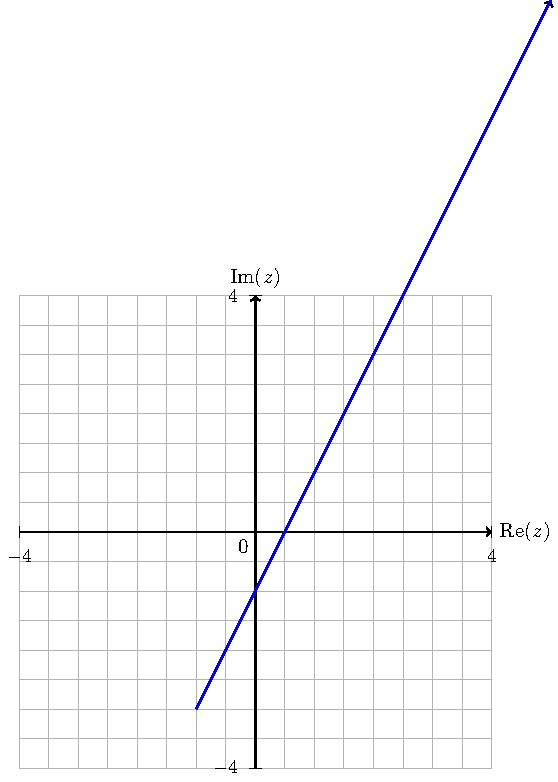
\includegraphics[width=.95\textwidth]{../../media/tikz/complex/ex-eq-01.pdf}
\end{minipage}
\end{split}
\end{equation*}
\sphinxAtStartPar
\sphinxstylestrong{2.} Trova i numeri complessi \(z\) che soddisfano \(z + \overline{z} = 2\).
\begin{equation*}
\begin{split}
\begin{minipage}[t]{.55\textwidth}
\begin{equation}2 \text{re}{z} = 2\end{equation}
\begin{equation}\text{re}{z}   = 1\end{equation}
\end{minipage}
\hspace{.05\textwidth}
\begin{minipage}[t]{.40\textwidth}
  \vspace{0pt}
  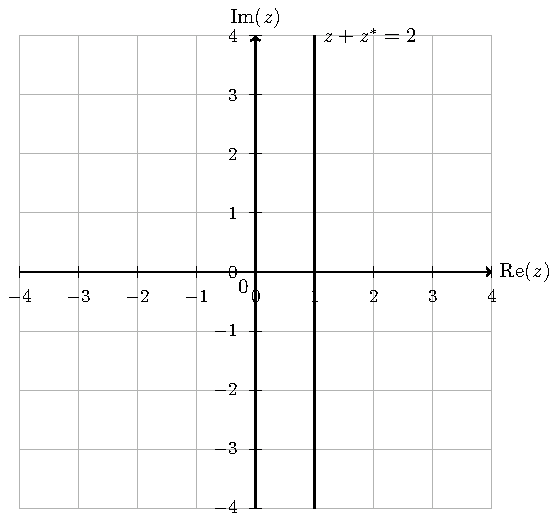
\includegraphics[width=.95\textwidth]{../../media/tikz/complex/ex-eq-02.pdf}
\end{minipage}
\end{split}
\end{equation*}
\sphinxAtStartPar
\sphinxstylestrong{3.} Risolvi \(z^2 - 2z + 5 = 0\) e calcola il modulo delle soluzioni.
\begin{equation*}
\begin{split}
\begin{minipage}[t]{.55\textwidth}
%
Usando la formula risolutiva per le equazioni di secondo grado,
\begin{equation} 
z = 1 \mp \sqrt{1-5} = 1 \mp i 2 \end{equation}
%
\textbf{Verifica.}
%
\begin{equation}\begin{aligned}
z^2  & = (1 \mp i 2)^2 = -3 \mp i 4 \\
-2 z & = -2 ( 1 \mp i 2 ) \\
+ 5  & = 5 \\
\hline 
& =  ( -3-2+5 ) + i(\mp 4 \pm 4) = 0 
\end{aligned}\end{equation}
%
\begin{equation}\text{re}{z}   = 1\end{equation}
\end{minipage}
\hspace{.05\textwidth}
\begin{minipage}[t]{.40\textwidth}
  \vspace{0pt}
  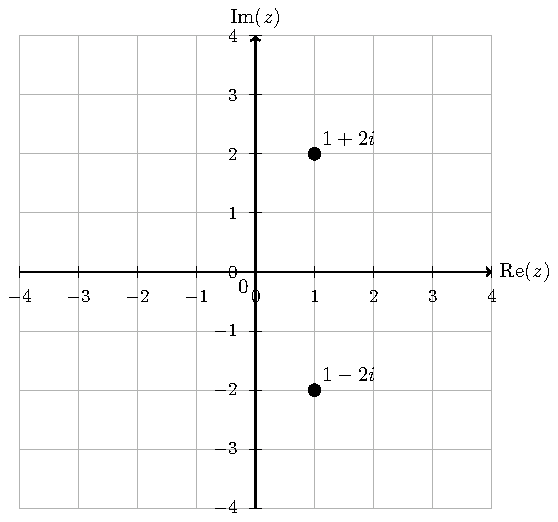
\includegraphics[width=.95\textwidth]{../../media/tikz/complex/ex-eq-03.pdf}
\end{minipage}
\end{split}
\end{equation*}
\sphinxAtStartPar
\sphinxstylestrong{4.} Risolvi \(|z - 3 + i| = 2\) e rappresenta graficamente le soluzioni.
\begin{equation*}
\begin{split}
\begin{minipage}[t]{.55\textwidth}
...
\end{minipage}
\hspace{.05\textwidth}
\begin{minipage}[t]{.40\textwidth}
  \vspace{0pt}
  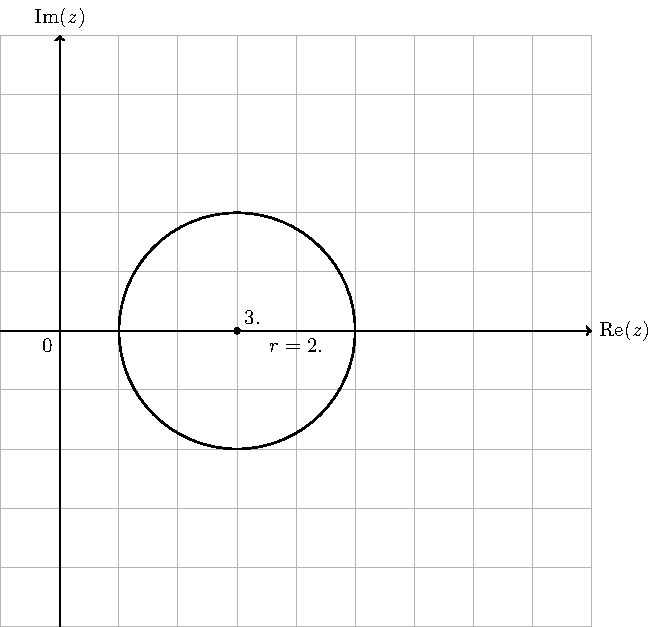
\includegraphics[width=.95\textwidth]{../../media/tikz/complex/ex-eq-04.pdf}
\end{minipage}
\end{split}
\end{equation*}
\sphinxAtStartPar
\sphinxstylestrong{5.} Trova i valori di \(z\) per cui \(z^3 = 27\).
\begin{equation*}
\begin{split}
\begin{minipage}[t]{.55\textwidth}
...
\end{minipage}
\hspace{.05\textwidth}
\begin{minipage}[t]{.40\textwidth}
  \vspace{0pt}
  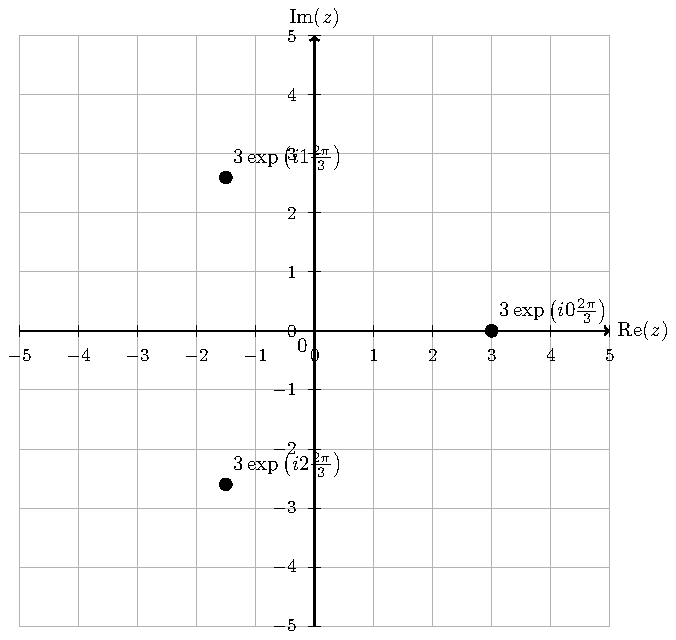
\includegraphics[width=.95\textwidth]{../../media/tikz/complex/ex-eq-05.pdf}
\end{minipage}
\end{split}
\end{equation*}
\sphinxAtStartPar
\sphinxstylestrong{6.} Risolvi \((z-1)^4 + 16 = 0\) e rappresenta graficamente le soluzioni nel piano complesso.
\begin{equation*}
\begin{split}
\begin{minipage}[t]{.55\textwidth}
...
\end{minipage}
\hspace{.05\textwidth}
\begin{minipage}[t]{.40\textwidth}
  \vspace{0pt}
  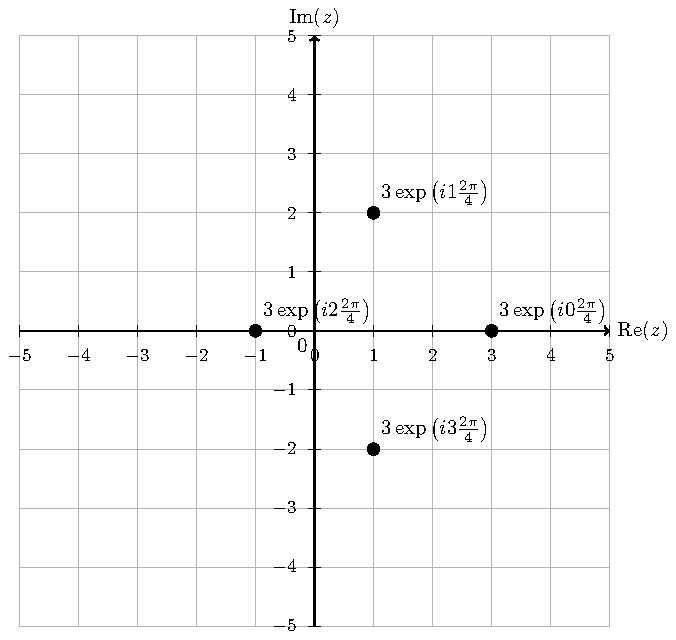
\includegraphics[width=.95\textwidth]{../../media/tikz/complex/ex-eq-06.pdf}
\end{minipage}
\end{split}
\end{equation*}
\sphinxAtStartPar
\sphinxstylestrong{7.} Risolvi \(|z - 2| = |z + 1|\) e descrivi il luogo geometrico delle soluzioni.
\begin{equation*}
\begin{split}
\begin{minipage}[t]{.55\textwidth}
...
\end{minipage}
\hspace{.05\textwidth}
\begin{minipage}[t]{.40\textwidth}
  \vspace{0pt}
  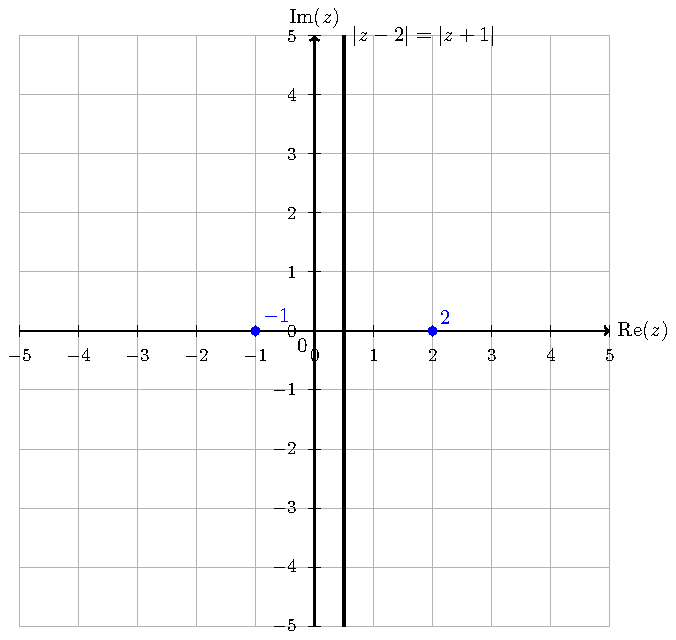
\includegraphics[width=.95\textwidth]{../../media/tikz/complex/ex-eq-07.pdf}
\end{minipage}
\end{split}
\end{equation*}
\sphinxAtStartPar
\sphinxstylestrong{8.} Trova le soluzioni di \(z^5 - 32 = 0\) e rappresentale in forma polare.

\sphinxAtStartPar
\sphinxstylestrong{9.} Determina i numeri complessi \(z\) per cui \(|z|^2 + |z - 2|^2 = 8\).

\sphinxAtStartPar
\sphinxstylestrong{10.} Risolvi \(|z + i| = 3\) per \(z \in \mathbb{C}\).

\sphinxAtStartPar
\sphinxstylestrong{11.} \(z^2 + 4 = 0\)

\sphinxAtStartPar
\sphinxstylestrong{12.} \(z^2 - 2z + 5 = 0\)

\sphinxAtStartPar
\sphinxstylestrong{13.} \(z^3 + 8 = 0\)

\sphinxAtStartPar
\sphinxstylestrong{14.} \(|z-2-i| = 2\)

\sphinxAtStartPar
\sphinxstylestrong{15.} \(|z-2-i| = |z-1|\)

\sphinxAtStartPar
\sphinxstylestrong{16.} \(z + \bar{z} = 1\)


\subsubsection{Disequazioni}
\label{\detokenize{ch/algebra/complex-algebra-sol:disequazioni}}\label{\detokenize{ch/algebra/complex-algebra-sol:math-hs-algebra-complex-problems-equations-ineq-sol}}
\sphinxAtStartPar
Soluzione degli {\hyperref[\detokenize{ch/algebra/complex-algebra-problems:math-hs-algebra-complex-problems-equations-ineq}]{\sphinxcrossref{\DUrole{std,std-ref}{esercizi su disequazioni con i numeri complessi}}}}

\sphinxAtStartPar
\sphinxstylestrong{1.} Trova i numeri complessi \(z\) che soddisfano \(|z| < 3\).
\begin{equation*}
\begin{split}
\begin{minipage}[t]{.55\textwidth}
...
\end{minipage}
\hspace{.05\textwidth}
\begin{minipage}[t]{.40\textwidth}
  \vspace{0pt}
  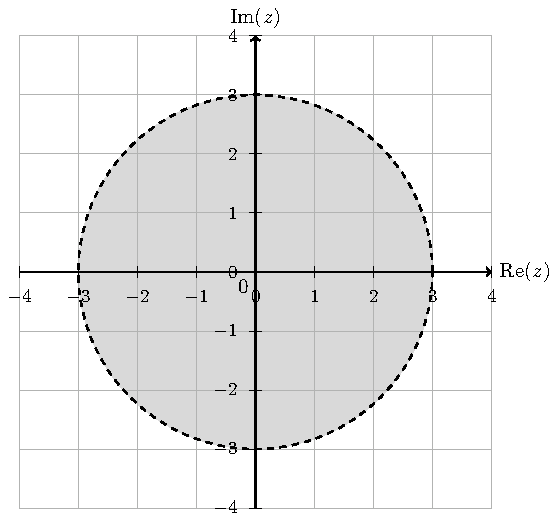
\includegraphics[width=.95\textwidth]{../../media/tikz/complex/ex-in-01.pdf}
\end{minipage}
\end{split}
\end{equation*}
\sphinxAtStartPar
\sphinxstylestrong{2.} Determina \(z\) per cui \(|z - 2| \geq 4\).
\begin{equation*}
\begin{split}
\begin{minipage}[t]{.55\textwidth}
...
\end{minipage}
\hspace{.05\textwidth}
\begin{minipage}[t]{.40\textwidth}
  \vspace{0pt}
  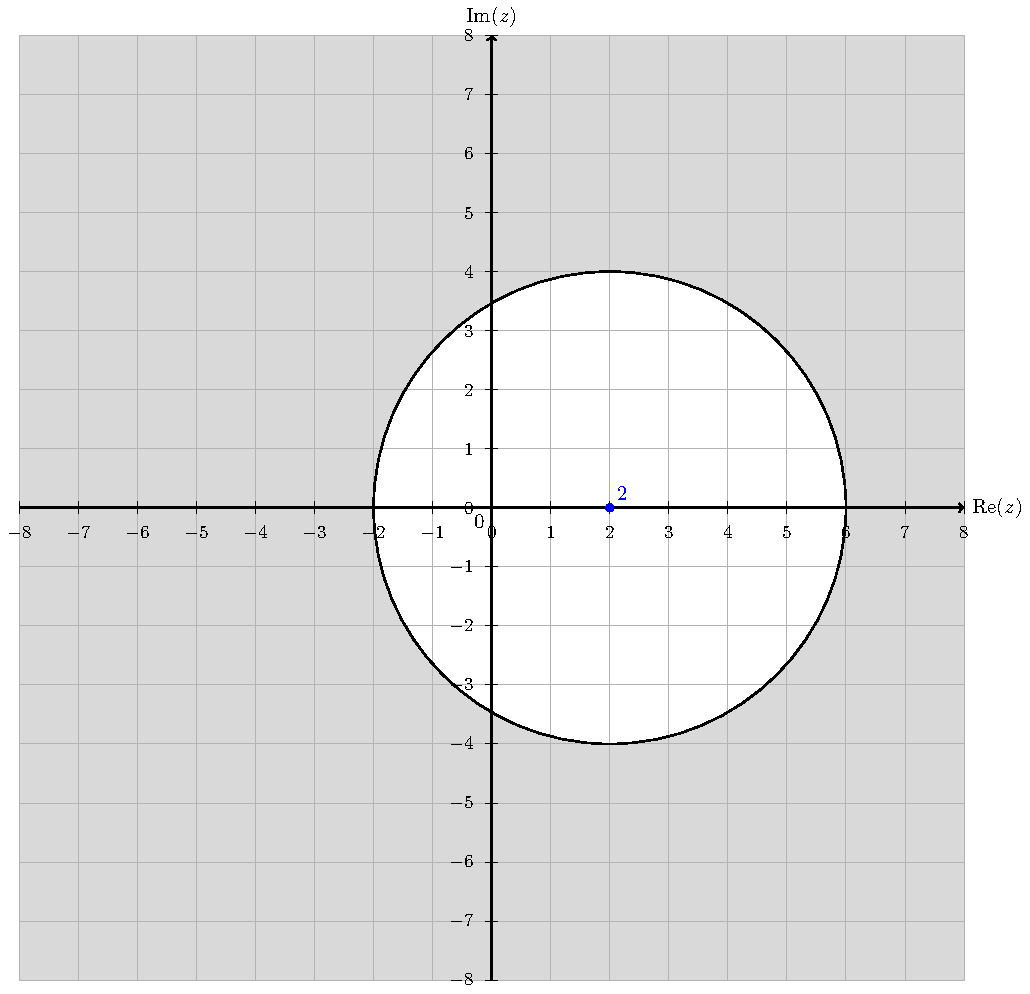
\includegraphics[width=.95\textwidth]{../../media/tikz/complex/ex-in-02.pdf}
\end{minipage}
\end{split}
\end{equation*}
\sphinxAtStartPar
\sphinxstylestrong{3.} Risolvi \(|z + i| \leq 2\).
\begin{equation*}
\begin{split}
\begin{minipage}[t]{.55\textwidth}
...
\end{minipage}
\hspace{.05\textwidth}
\begin{minipage}[t]{.40\textwidth}
  \vspace{0pt}
  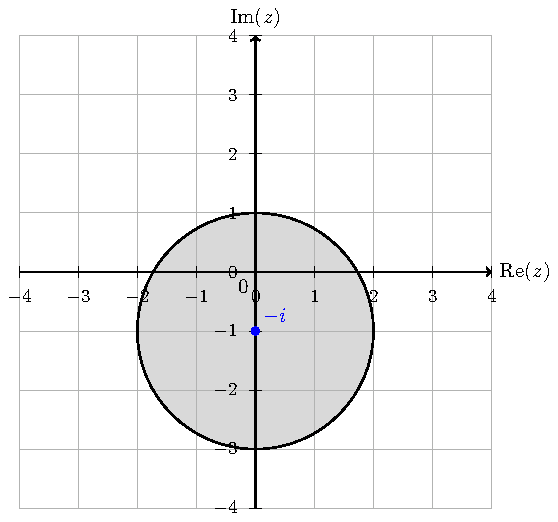
\includegraphics[width=.95\textwidth]{../../media/tikz/complex/ex-in-03.pdf}
\end{minipage}
\end{split}
\end{equation*}
\sphinxAtStartPar
\sphinxstylestrong{4.} Trova \(z\) tali che \(\text{Re}(z) > \text{Im}(z)\).
\begin{equation*}
\begin{split}
\begin{minipage}[t]{.55\textwidth}
...
\end{minipage}
\hspace{.05\textwidth}
\begin{minipage}[t]{.40\textwidth}
  \vspace{0pt}
  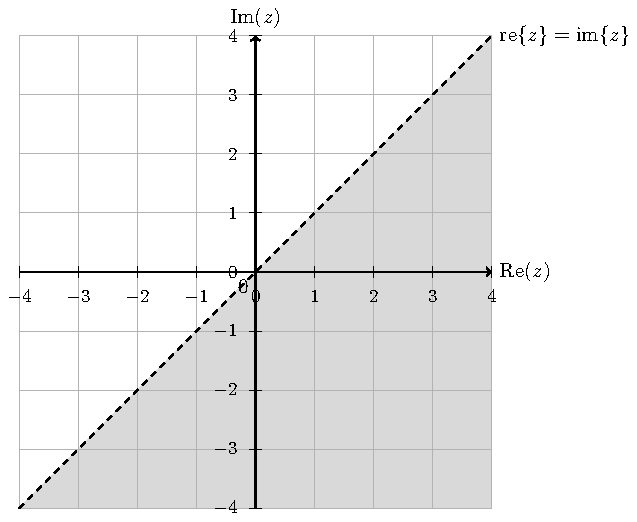
\includegraphics[width=.95\textwidth]{../../media/tikz/complex/ex-in-04.pdf}
\end{minipage}
\end{split}
\end{equation*}
\sphinxAtStartPar
\sphinxstylestrong{5.} Risolvi \(|z - 1| > |z + 1|\).
\begin{equation*}
\begin{split}
\begin{minipage}[t]{.55\textwidth}
...
\end{minipage}
\hspace{.05\textwidth}
\begin{minipage}[t]{.40\textwidth}
  \vspace{0pt}
  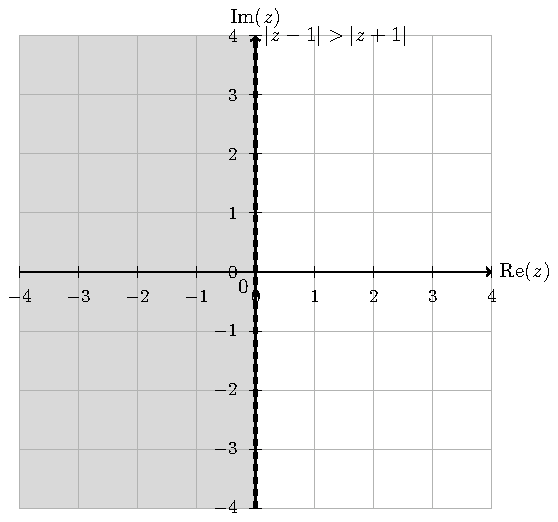
\includegraphics[width=.95\textwidth]{../../media/tikz/complex/ex-in-05.pdf}
\end{minipage}
\end{split}
\end{equation*}
\sphinxAtStartPar
\sphinxstylestrong{6.} Determina il luogo geometrico di \(z\) per cui \(|z| - |z-2| \leq 1\).
\begin{equation*}
\begin{split}
\begin{minipage}[t]{.55\textwidth}
La condizione corrisponde alla ricerca dei punti del piano in una zona del piano delimitata da un ramo dell'iperbole con fuochi $F_1 \equiv (0,0)$, $F_2(2,0)$ e con differenza delle distanze $2 a = 1$. La distanza dei due fuochi è $2c = 2$. I coefficienti che definiscono l'iperbole sono quindi
%
\begin{equation}
  a = \frac{1}{2} \ , \quad c = 1 \ , \quad b = \sqrt{c^2-a^2} = \frac{\sqrt{3}}{2} \ ,
\end{equation}
%
il centro è $C \equiv \left(1,0 \right)$ e l'eccentricità $e = \frac{c}{a} = 2 > 1$.
%
Le coordinate dei punti dell'iperbole possono essere scritte in forma parametrica come
%
\begin{equation} P - C = \hat{x} a \cosh \theta + \hat{y} b \sinh \theta \end{equation}
%
o usando i numeri complessi,
%
\begin{equation} z(\theta) = 1 + a \cosh \theta + i b \sinh \theta \end{equation}
%
\end{minipage}
\hspace{.05\textwidth}
\begin{minipage}[t]{.40\textwidth}
  \vspace{0pt}
  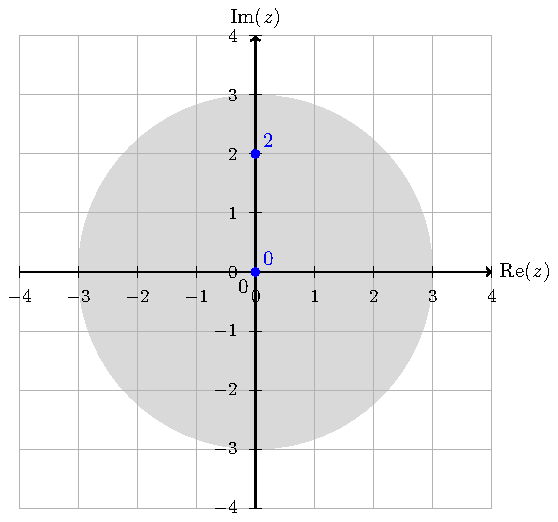
\includegraphics[width=.95\textwidth]{../../media/tikz/complex/ex-in-06.pdf}
\end{minipage}
\end{split}
\end{equation*}
\sphinxAtStartPar
\sphinxstylestrong{7.} Risolvi \(\text{Re}(z) + \text{Im}(z) \leq 2\).
\begin{equation*}
\begin{split}
\begin{minipage}[t]{.55\textwidth}
...
\end{minipage}
\hspace{.05\textwidth}
\begin{minipage}[t]{.40\textwidth}
  \vspace{0pt}
  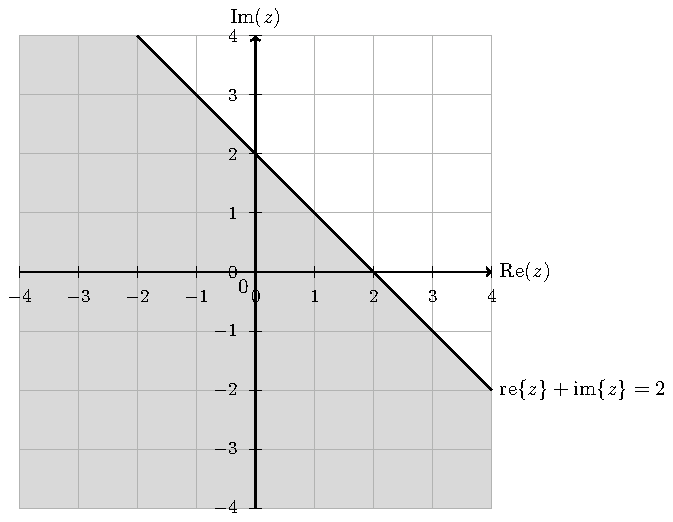
\includegraphics[width=.95\textwidth]{../../media/tikz/complex/ex-in-07.pdf}
\end{minipage}
\end{split}
\end{equation*}
\sphinxAtStartPar
\sphinxstylestrong{8.} Trova \(z\) tali che \(|z| + |z - 1| \leq 5\).
\begin{equation*}
\begin{split}
\begin{minipage}[t]{.55\textwidth}
La condizione corrisponde alla ricerca dei punti del piano contenuti nella regione delimitata dall'ellisse con fuochi $F_1 \equiv (0,0)$, $F_2(1,0)$ e con somma delle distanze $2 a = 5$. La distanza dei due fuochi è $2c = 1$. I coefficienti che definiscono l'ellisse sono quindi
%
\begin{equation}
  a = \frac{5}{2} \ , \quad c = \frac{1}{2} \ , \quad b = \sqrt{a^2-c^2} = \frac{\sqrt{24}}{2} = \sqrt{6}
\end{equation}
%
il centro è $C \equiv \left(\frac{1}{2},0 \right)$ e l'eccentricità $e = \frac{c}{a} = \frac{1}{5}$.
%
Le coordinate dei punti dell'ellisse possono essere scritte in forma parametrica come
%
\begin{equation} P - C = \hat{x} a \cos \theta + \hat{y} b \sin \theta \end{equation}
%
o usando i numeri complessi,
%
\begin{equation} z(\theta) = \frac{1}{2} + a \cos \theta + i b \sin \theta \end{equation}
%
\end{minipage}
\hspace{.05\textwidth}
\begin{minipage}[t]{.40\textwidth}
  \vspace{0pt}
  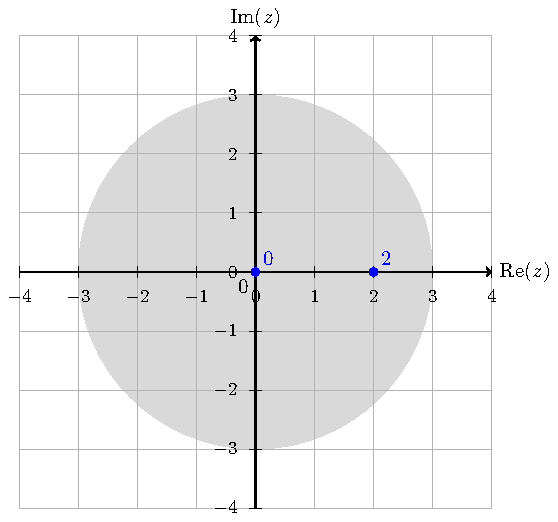
\includegraphics[width=.95\textwidth]{../../media/tikz/complex/ex-in-08.pdf}
\end{minipage}
\end{split}
\end{equation*}
\sphinxAtStartPar
\sphinxstylestrong{9.} Trova \(z\) tali che \(|z+i| + |z - 1| \leq 5\).
\begin{equation*}
\begin{split}
\begin{minipage}[t]{.55\textwidth}
La condizione corrisponde alla ricerca dei punti del piano contenuti nella regione delimitata dall'ellisse con fuochi $F_1 \equiv (0,-1)$, $F_2(1,0)$ e con somma delle distanze $2 a = 5$. La distanza dei due fuochi è $2c = \sqrt{2}$. I coefficienti che definiscono l'ellisse sono quindi
%
\begin{equation}
  a = \frac{5}{2} \ , \quad c = \frac{\sqrt{2}}{2} \ , \quad b = \sqrt{a^2-c^2} = \frac{\sqrt{23}}{2} 
\end{equation}
%
il centro è $C \equiv \left(\frac{1}{2}, -\frac{1}{2} \right)$ e l'eccentricità $e = \frac{c}{a} = \frac{\sqrt{2}}{5}$.
%
Le coordinate dei punti dell'ellisse possono essere scritte in forma parametrica come
%
\begin{equation} P - C = \hat{x} a \cos \theta + \hat{y} b \sin \theta \end{equation}
%
o usando i numeri complessi,
%
\begin{equation} z(\theta) = \frac{1}{2} + a \cos \theta + i \left[ - \frac{1}{2} + b \sin \theta \right] \end{equation}
%
%
\end{minipage}
\hspace{.05\textwidth}
\begin{minipage}[t]{.40\textwidth}
  \vspace{0pt}
  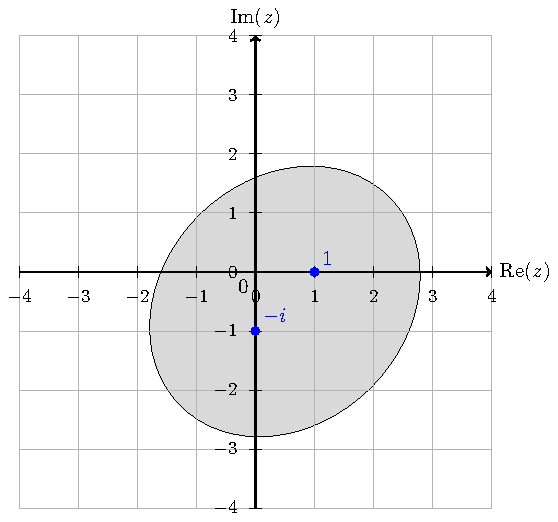
\includegraphics[width=.95\textwidth]{../../media/tikz/complex/ex-in-09.pdf}
\end{minipage}
\end{split}
\end{equation*}
\sphinxAtStartPar
\sphinxstylestrong{10.} Risolvi \(|z - i| \geq |z + 2|\).
\begin{equation*}
\begin{split}
\begin{minipage}[t]{.55\textwidth}
...
\end{minipage}
\hspace{.05\textwidth}
\begin{minipage}[t]{.40\textwidth}
  \vspace{0pt}
  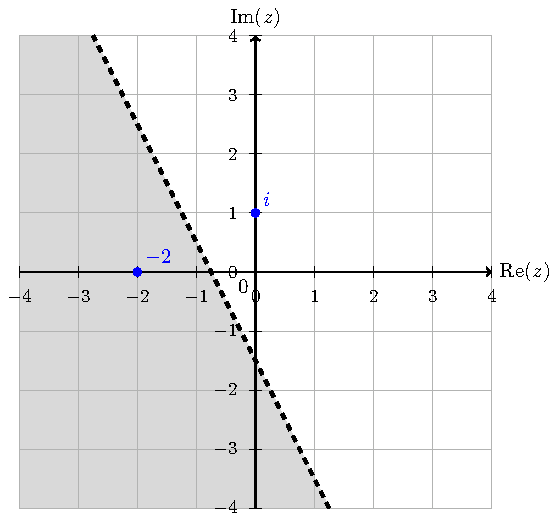
\includegraphics[width=.95\textwidth]{../../media/tikz/complex/ex-in-10.pdf}
\end{minipage}
\end{split}
\end{equation*}
\sphinxAtStartPar
\sphinxstylestrong{11.} Determina il luogo geometrico di \(z\) per cui \(|z| - |z-2| \leq 3\).

\sphinxAtStartPar
Si riorganizza l’equazione per confrontare due termini non\sphinxhyphen{}negativi,
\begin{equation*}
\begin{split}
  |z| \leq 3 + |z-2| \ .
\end{split}
\end{equation*}
\sphinxAtStartPar
Usando una rappresentazione cartesiana, \(z = x + i y\),
\begin{equation*}
\begin{split}\begin{aligned}
  & x^2 + y^2 \leq 9 + (x-2)^2 + y^2 + 6\sqrt{(x-2)^2+y^2} \\
  & x^2 + y^2 \leq 9 + x^2 - 4x + 4 + y^2 + 6\sqrt{(x-2)^2+y^2} \\
  & 4x - 13   \leq 6\sqrt{(x-2)^2+y^2} \\
\end{aligned}\end{split}
\end{equation*}
\sphinxAtStartPar
Ora, si osserva che il termine di destra è non\sphinxhyphen{}negativo per ogni valore di \(x\), \(y\). Il termine di sinistra può avere segno positivo o negativo. Si discutono quindi i due casi:
\begin{itemize}
\item {} 
\sphinxAtStartPar
\(4x - 13 \leq 0\): la disequazione è sempre soddisfatta poiché il termine di sinistra è non\sphinxhyphen{}positivo, il termine di destra è non\sphinxhyphen{}negativo e deve essere maggiore \sphinxstyleemphasis{o uguale} al termine di sinitra. Questo è quindi sempre vero, nel caso in cui \(4 x - 13 \leq 0\)

\item {} 
\sphinxAtStartPar
\(4x - 13 > 0\): in questo caso entrambi i termini sono non negativi, e quindi si può elevare al quadrato per «eliminare» la radice quadrata.
\begin{equation*}
\begin{split}\begin{aligned}
    & 16x^2 - 104 x + 169 \leq 36 x^2 - 144 x + 144 + 36 y^2 \\
    & 0 \leq 20 x^2 - 40 x - 25 + 36 y^2 \\
    & 0 \leq 20 ( x^2 - 2 x + 1 ) - 45 + 36 y^2 \\
    &  \frac{(x-1)^2}{\frac{45}{20}} + \frac{y^2}{\frac{45}{36}} \geq 1 \ ,
  \end{aligned}\end{split}
\end{equation*}
\sphinxAtStartPar
e questa disequazione è soddisfatta per tutti i punti esterni all’ellisse con centro \((1,0)\) e semi\sphinxhyphen{}assi
\begin{equation*}
\begin{split}\begin{aligned}
    a & = \sqrt{\frac{45}{20}} = \sqrt{\frac{9}{4}} = \frac{3}{2} \\
    b & = \sqrt{\frac{45}{36}} = \sqrt{\frac{5}{4}} = \frac{\sqrt{5}}{2} \\
  \end{aligned}\end{split}
\end{equation*}
\sphinxAtStartPar
Il punto con parte reale minima per la quale la disequazione smette di essere soddisfatta è il punto estremo sul semiasse maggiore, \(z = z_c + a = 1 + \frac{3}{2} = \frac{5}{2}\). Questo numero è minore di \(\frac{13}{4}\), valore limite di \(x\) di questo secondo caso. Quindi la disequazione è sempre soddisfatta per tutti gli \(x > \frac{13}{4}\).

\end{itemize}

\sphinxAtStartPar
La disequazione risulta quindi soddisfatta sempre in entrambi i casi, e quindi risulta sempre soddisfatta in tutto il piano complesso, cioè vale \(\forall z \in \mathbb{C}\).
\begin{equation*}
\begin{split}
\begin{minipage}[t]{.45\textwidth}
  \vspace{0pt}
  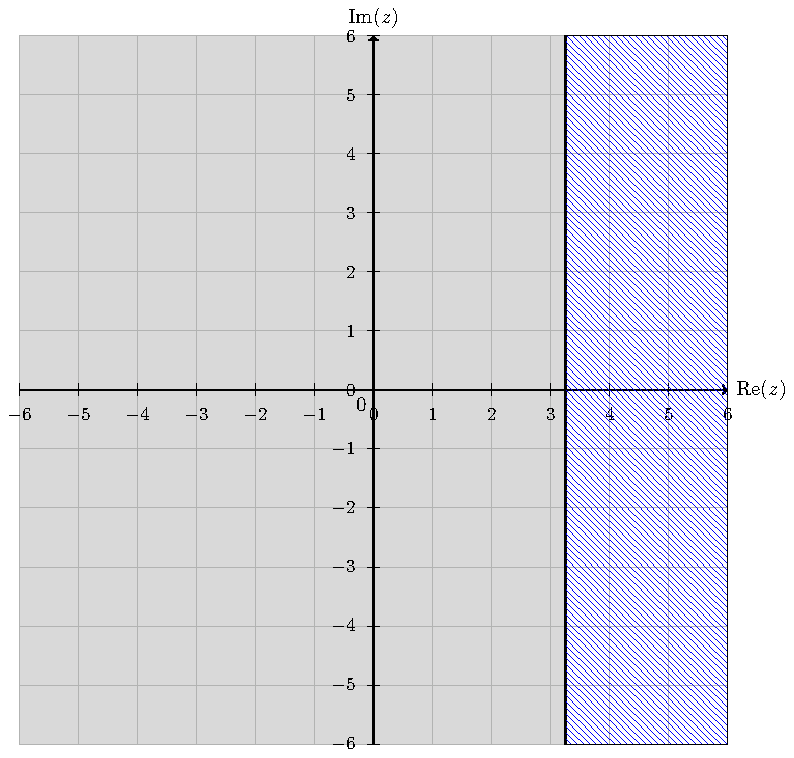
\includegraphics[width=.95\textwidth]{../../media/tikz/complex/ex-in-11.pdf}
\end{minipage}
\hspace{.05\textwidth}
\begin{minipage}[t]{.45\textwidth}
  \vspace{0pt}
  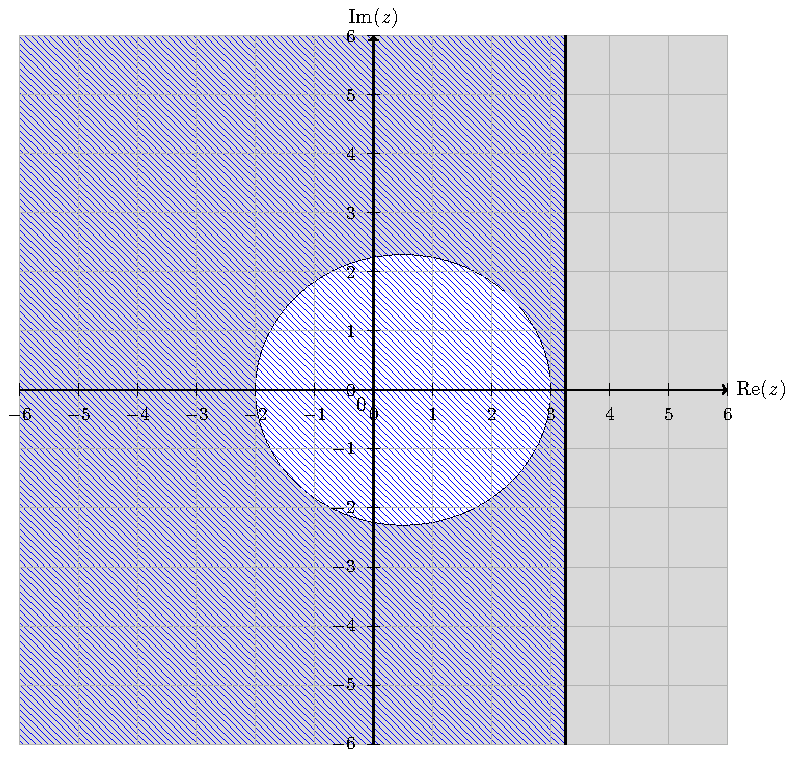
\includegraphics[width=.95\textwidth]{../../media/tikz/complex/ex-in-11-a.pdf}
\end{minipage}
\end{split}
\end{equation*}

\subsubsection{Sistemi}
\label{\detokenize{ch/algebra/complex-algebra-sol:sistemi}}\label{\detokenize{ch/algebra/complex-algebra-sol:math-hs-algebra-complex-problems-equations-sys-sol}}
\sphinxAtStartPar
Soluzione degli {\hyperref[\detokenize{ch/algebra/complex-algebra-problems:math-hs-algebra-complex-problems-equations-sys}]{\sphinxcrossref{\DUrole{std,std-ref}{esercizi su sistemi di equazioni con i numeri complessi}}}}

\sphinxAtStartPar
\sphinxstylestrong{1.} Risolvere \(\begin{cases} z + z^* = 6 \\ |z| = 5 \end{cases}\)
\begin{equation*}
\begin{split}
\begin{minipage}[t]{.55\textwidth}
  \vspace{0pt}
La prima equazione si riduce a $2 \text{re}\{z\} = 6$. Usando la rappresentazione cartesiana, $z = x + i y$, il sistema può essere riscritto come
%
\begin{equation}\begin{cases}
  x = 3 \\
  \sqrt{x^2 +y^2} = 5
\end{cases}\end{equation}
%
Sostituendo la prima nella seconda si trova $\sqrt{9 + y^2} = 5$; elevando al quadrato i due numeri positivi, $y^2 = 25-9=16$ e quindi $y = \mp 4$. Il problema ha quindi due soluzioni
%
\begin{equation}\begin{aligned}
  z_1 & = 3 - i 4 \\
  z_2 & = 3 + i 4
\end{aligned}\end{equation}
%
\textbf{Interpretazione grafica.} Le due equazioni corrispondono all'equazione della retta di equazione $x = 3$ e della circonferenza centrata nell'origine di raggio $5$. La soluzione del sistema coincide con la ricerca dei punti di intersezione di queste due curve.
%
\end{minipage}
\hspace{.05\textwidth} %
\begin{minipage}[t]{.40\textwidth}
  \vspace{0pt}
  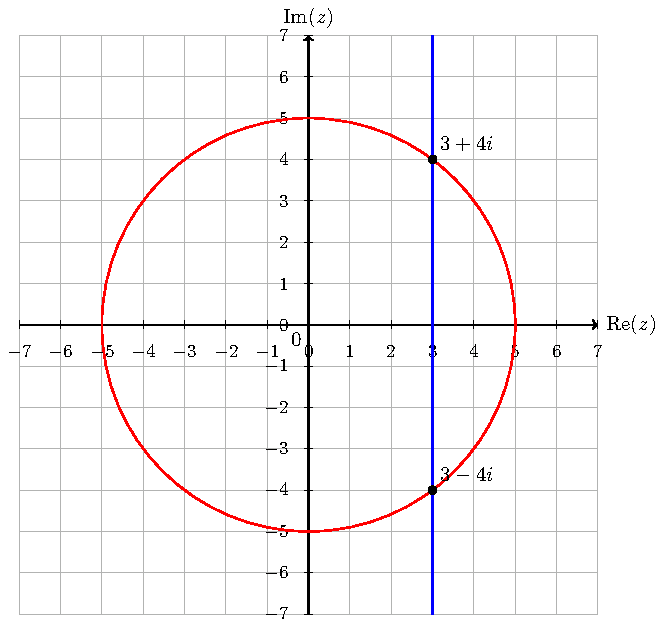
\includegraphics[width=.95\textwidth]{../../media/tikz/complex/ex-sy-01.pdf}
\end{minipage}
\end{split}
\end{equation*}
\sphinxAtStartPar
\sphinxstylestrong{2.} Trova \(z_1\) e \(z_2\) che soddisfano il sistema:\\
\(\begin{cases} 
   |z_1| = 3 \\
   z_1 z_2 = 9 
   \end{cases}\)

\sphinxAtStartPar
\sphinxstylestrong{3.} Risolvi il sistema:\\
\(\begin{cases} 
   z^2 + w^2 = 5 \\
   z w = 4 
   \end{cases}\)

\sphinxAtStartPar
\sphinxstylestrong{4.} Determina le soluzioni del sistema:\\
\(\begin{cases} 
   |z| = 4 \\
   z + \overline{z} = 6 
   \end{cases}\)

\sphinxAtStartPar
\sphinxstylestrong{5.} Risolvi il sistema:\\
\(\begin{cases} 
   z^3 + w = 1 \\
   z w^3 = -1 
   \end{cases}\)

\sphinxAtStartPar
\sphinxstylestrong{6.} Trova \(z\) e \(w\) per il sistema:\\
\(\begin{cases} 
   z^2 + w^2 = 7 \\
   z + w = 3 
   \end{cases}\)

\sphinxAtStartPar
\sphinxstylestrong{7.} Risolvi il sistema:\\
\(\begin{cases} 
   |z| = 2 \\
   z + w = 0 
   \end{cases}\)

\sphinxAtStartPar
\sphinxstylestrong{8.} Trova \(z\) e \(w\) che soddisfano il sistema:\\
\(\begin{cases} 
   z w = 1 \\
   z - w = i 
   \end{cases}\)

\sphinxAtStartPar
\sphinxstylestrong{9.} Determina le soluzioni del sistema:\\
\(\begin{cases} 
   z^2 + \overline{z}^2 = 8 \\
   z \cdot \overline{z} = 9 
   \end{cases}\)

\sphinxAtStartPar
\sphinxstylestrong{10.} Risolvi il sistema:\\
\(\begin{cases} 
    z + w = 5 + i \\
    z \cdot w = 6 - i 
    \end{cases}\)

\sphinxstepscope


\section{Note e dimostrazioni}
\label{\detokenize{ch/algebra/complex-algebra-notes:note-e-dimostrazioni}}\label{\detokenize{ch/algebra/complex-algebra-notes:math-hs-algebra-complex-notes}}\label{\detokenize{ch/algebra/complex-algebra-notes::doc}}



\subsection{Formula di de Moivre}
\label{\detokenize{ch/algebra/complex-algebra-notes:formula-di-de-moivre}}\label{\detokenize{ch/algebra/complex-algebra-notes:math-hs-algebra-complex-notes-demoivre}}
\sphinxAtStartPar
Qui si dimostra la formula di de Moivre \eqref{equation:ch/algebra/complex-algebra:complex:demoivre}.
\begin{equation*}
\begin{split}(\cos x + i \sin x)^n = \cos(nx) + i \sin(nx) \ , \quad n \in \mathbb{Z}\end{split}
\end{equation*}\subsubsection*{Dimostrazione per induzione}

\sphinxAtStartPar
Per \(n \in \mathbb{N}\), si procede per induzione \sphinxstylestrong{todo} \sphinxstyleemphasis{aggiungere i capitoli sulla logica? E un riferimento ad essi?} Per \(n = 1\) la formula di de Moivre si riduce a un’identità. Supponiamo quindi che sia valida per un intero \(n > 1\) e verifichiamo se questo implica che sia valida anche per \(n+1\)
\begin{equation*}
\begin{split}\begin{aligned}
  (\cos x + i \sin x)^{n+1} & = (\cos x + i \sin x)^n \, (\cos x + i \sin x) = \\
                            & = \left(\cos (nx)+ i \sin (nx) \right) \, (\cos x + i \sin x) = \\
                            & = \cos(nx) \cos x - \sin(nx) \sin x + i \left( \cos(nx) \sin x + \sin(nx) \cos x \right) = \\
                            & = \cos( (n+1)x ) + i \sin( (n+1) x ) \ .
\end{aligned}\end{split}
\end{equation*}
\sphinxAtStartPar
Per \(n = 0\), la formula di de Moivre si riduce all’identità \(1 \equiv 1\).

\sphinxAtStartPar
Per \(m := -n \in \mathbb{N}\), la formula di de Moivre può essere verificata usando la formula di de Moivre per \(m > 0\) e razionalizzando la frazione,
\begin{equation*}
\begin{split}\begin{aligned}
  \left( \cos x + i \sin x \right)^{n} & = \frac{1}{\left( \cos x + i \sin x \right)^m} = \\
   & = \frac{1}{\left( \cos (m x) + i \sin (m x) \right)} = \\
   & = \frac{\cos( m x) - i \sin (m x)}{\underbrace{\cos^2(mx) + \sin^2(mx)}_{=1}} = \cos(mx) - i \sin(mx) = \cos(nx) + i \sin(nx) \ .
\end{aligned}\end{split}
\end{equation*}

\subsection{Esponenziale complesso}
\label{\detokenize{ch/algebra/complex-algebra-notes:esponenziale-complesso}}\label{\detokenize{ch/algebra/complex-algebra-notes:math-hs-algebra-complex-notes-complex-exp}}
\sphinxAtStartPar
Estendendo la definizione di funzione esponenziale \(e^x\) ai numeri complessi, si può scrivere
\begin{equation}\label{equation:ch/algebra/complex-algebra-notes:complex:complex-exp:notes}
\begin{split}e^z = \sum_{n = 0}^{+\infty} \frac{z^n}{n!} = \lim_{n \rightarrow +\infty} \left( 1 + \frac{z}{n} \right)^n\end{split}
\end{equation}



\subsection{Formula di Eulero}
\label{\detokenize{ch/algebra/complex-algebra-notes:formula-di-eulero}}\label{\detokenize{ch/algebra/complex-algebra-notes:math-hs-algebra-complex-notes-euler}}
\sphinxAtStartPar
Per esponenti reali, vale
\begin{equation*}
\begin{split}e^{i x} = \cos x + i \sin x\end{split}
\end{equation*}\subsubsection*{Dimostrazione usando la definizione come limite della successione}

\sphinxAtStartPar
L’esponenziale complesso può essere scritto come limite della successione con termini,
\begin{equation*}
\begin{split}a_n = \left( 1 + \frac{z}{n} \right)^n = \left( 1 + \frac{x}{n} + i \frac{y}{n} \right)^n\end{split}
\end{equation*}
\sphinxAtStartPar
per \(n \rightarrow +\infty\). Usando le trasformazioni tra la rappresentazione cartesiana e la rappresentazione polare
\begin{equation*}
\begin{split}\begin{cases}
  \text{re}\{a_n\} = 1 + \frac{x}{n} = r_n \cos \theta_n \\
  \text{im}\{a_n\} = \frac{y}{n} = r_n \sin \theta_n
\end{cases}\end{split}
\end{equation*}\begin{equation*}
\begin{split}\begin{cases}
  r_n = \sqrt{ \left(\text{re}\{a_n\}\right)^2 + \left(\text{im}\{a_n\}\right)^2 } =  \sqrt{\left(1+ \frac{x}{n}\right)^2 + \left(\frac{y}{n}\right)^2} \\
  \tan \theta_n = \frac{\text{im}\{a_n\}}{\text{re}\{a_n\}} = \frac{\frac{y}{n}}{1 + \frac{x}{n}} = \frac{y}{x + n}_n
\end{cases}\end{split}
\end{equation*}


\sphinxAtStartPar
e la {\hyperref[\detokenize{ch/algebra/complex-algebra-notes:math-hs-algebra-complex-notes-demoivre}]{\sphinxcrossref{\DUrole{std,std-ref}{formula di de Moivre}}}},
\begin{equation*}
\begin{split}( \cos x + i \sin x)^n = \cos( n x ) + i \sin ( n x )\end{split}
\end{equation*}
\sphinxAtStartPar
si può scrivere il termine \(a_n\)
\begin{equation*}
\begin{split}\begin{aligned}
  a_n & = \left( 1 + \frac{x}{n} + i \frac{y}{n} \right)^n = \\
      & = \left( r_n \cos \theta_n + i r_n \sin \theta \right)^n = \\
      & = r_n^n \cdot \left[ \cos ( n \theta_n ) + i \sin (n \theta_n) \right]
\end{aligned}\end{split}
\end{equation*}
\sphinxAtStartPar
Per \(n \rightarrow \infty\), \(\tan \theta_n \rightarrow 0\) e quindi vale l’approssimazione asintotica \(\tan \theta_n \sim \theta_n\)
\begin{equation*}
\begin{split}\theta_n \sim \tan \theta_n = \frac{y}{x+n} \sim \frac{y}{n}\end{split}
\end{equation*}\begin{equation*}
\begin{split}n \theta_n \sim y\end{split}
\end{equation*}
\sphinxAtStartPar
mentre è possibile studiare il limite del modulo, riscrivendolo come
\begin{equation*}
\begin{split}\begin{aligned}
  r_n^n & = \left[ \left( 1 + \frac{x}{n} \right)^2 + \left( \frac{y}{n} \right)^2 \right]^{\frac{n}{2}} = \\
        & = \left( 1 + \frac{x}{n} \right)^{n} \left[ 1 + \left(\frac{y}{n+x}\right)^2 \right]^{\frac{n}{2}} = \\
\end{aligned}\end{split}
\end{equation*}
\sphinxAtStartPar
Il primo fattore è asintotico a \(e^x\),
\begin{equation*}
\begin{split}\left( 1 + \frac{x}{n} \right)^n \sim e^x \ .\end{split}
\end{equation*}
\sphinxAtStartPar
Il secondo fattore, con il «completamento della definizione di esponenziale», può essere riscritto come
\begin{equation*}
\begin{split}\left[ 1 + \left(\frac{y}{n+x}\right)^2 \right]^{\frac{n}{2}} = \left\{ \left[ 1 + \left(\frac{y}{n+x}\right)^2 \right]^{\left(\frac{n+x}{y}\right)^2} \right\}^{\frac{n y^2}{2(n+x)^2}} \sim e^0 = 1 \ .\end{split}
\end{equation*}
\sphinxAtStartPar
Il termine \(r_n^n\) tende quindi a \(e^x\).

\sphinxAtStartPar
Il limite dei termini \(a_n\) della successione che definisce l’esponenziale complesso può quindi essere scritto come
\begin{equation*}
\begin{split}\begin{aligned}
  e^z & = \lim_{n \rightarrow +\infty} a_n = \\
      & = \lim_{n \rightarrow +\infty} r_n (\cos(n\theta) + i \sin(n\theta)) =  & (\lim_{n\rightarrow +\infty} r_n = e^x, \lim_{n \rightarrow + \infty} n \theta = y)\\
      & = e^x \left( \cos y + i \sin y \right) \ .
\end{aligned}\end{split}
\end{equation*}
\sphinxAtStartPar
Usando la proprietà delle potenze estesa ai numeri complessi,
\begin{equation*}
\begin{split}e^x \left( \cos y + i \sin y \right) = e^z = e^{x + iy} = e^x \, e^{i y} \ ,
\end{split}
\end{equation*}
\sphinxAtStartPar
dall’arbitrarietà del valore \(x\), risulta dimostrata la formula di Eulero,
\begin{equation*}
\begin{split}e^{iy} = \cos y + i \sin y \ .\end{split}
\end{equation*}
\sphinxAtStartPar
per esponenti reali \(y \in \mathbb{R}\).
\subsubsection*{Dimostrazione usando la definizione come serie}

\sphinxAtStartPar
L’identità di Eulero può essere dimostrata (\sphinxstylestrong{todo} \sphinxstyleemphasis{bisogna verificare la convergenza (uniforme) delle serie?}) confrontando le {\hyperref[\detokenize{ch/infinitesimal_calculus/derivatives:infinitesimal-calculus-derivatives-taylor}]{\sphinxcrossref{\DUrole{std,std-ref}{serie polinomiali di Taylor}}}} delle funzioni \(\cos x\), \(\sin x\) definite sui numeri reali, \(x \in \mathbb{R}\)
\begin{equation*}
\begin{split}\begin{aligned}
  \cos x & = 1 - \frac{x^2}{2!} + \frac{x^4}{4!} + \dots \\
  \sin x & = x - \frac{x^3}{3!} + \frac{x^5}{5!} + \dots \\
\end{aligned}\end{split}
\end{equation*}
\sphinxAtStartPar
con la serie che definisce l’esponenziale complesso,
\begin{equation*}
\begin{split}
  e^z & = 1 + z + \frac{z^2}{2!} + \frac{z^3}{3!} + \frac{z^4}{4!} + \frac{z^5}{5!} + \dots \\
\end{split}
\end{equation*}
\sphinxAtStartPar
valutata in \(z = i x \in \mathbb{C}\)
\begin{equation*}
\begin{split}\begin{aligned}
  e^{i x} 
      & = 1 + i x + \frac{(i x)^2}{2!} + \frac{(i x)^3}{3!} + \frac{(i x)^4}{4!} + \frac{(i x)^5}{5!} + \dots = \\
      & = 1 - \frac{x^2}{2!} + \frac{x^4}{4!} \dots + i \left[ x - \frac{x^3}{3!} + \frac{x^5}{5!}  + \dots \right] = \\
      & = \cos x + i \sin x \ .
\end{aligned}\end{split}
\end{equation*}

\subsection{Altre operazioni e funzioni a variabile complessa}
\label{\detokenize{ch/algebra/complex-algebra-notes:altre-operazioni-e-funzioni-a-variabile-complessa}}\label{\detokenize{ch/algebra/complex-algebra-notes:math-hs-algebra-complex-notes-fun}}

\subsubsection{Potenza}
\label{\detokenize{ch/algebra/complex-algebra-notes:potenza}}\label{\detokenize{ch/algebra/complex-algebra-notes:math-hs-algebra-complex-notes-fun-power}}

\subsubsection{Esponenziale}
\label{\detokenize{ch/algebra/complex-algebra-notes:esponenziale}}\label{\detokenize{ch/algebra/complex-algebra-notes:math-hs-algebra-complex-notes-fun-exp}}

\subsubsection{Logaritmo}
\label{\detokenize{ch/algebra/complex-algebra-notes:logaritmo}}\label{\detokenize{ch/algebra/complex-algebra-notes:math-hs-algebra-complex-notes-fun-log}}
\sphinxstepscope

\begin{sphinxuseclass}{sd-container-fluid}
\begin{sphinxuseclass}{sd-sphinx-override}
\begin{sphinxuseclass}{sd-p-0}
\begin{sphinxuseclass}{sd-mt-2}
\begin{sphinxuseclass}{sd-mb-4}
\begin{sphinxuseclass}{sd-row}
\begin{sphinxuseclass}{sd-row-cols-2}
\begin{sphinxuseclass}{sd-gx-2}
\begin{sphinxuseclass}{sd-gy-1}
\begin{sphinxuseclass}{sd-col}
\begin{sphinxuseclass}{sd-d-flex-row}
\begin{sphinxuseclass}{sd-align-minor-center}
\begin{sphinxuseclass}{sd-container-fluid}
\begin{sphinxuseclass}{sd-sphinx-override}
\begin{sphinxuseclass}{sd-row}
\begin{sphinxuseclass}{sd-row-cols-2}
\begin{sphinxuseclass}{sd-row-cols-xs-2}
\begin{sphinxuseclass}{sd-row-cols-sm-3}
\begin{sphinxuseclass}{sd-row-cols-md-3}
\begin{sphinxuseclass}{sd-row-cols-lg-3}
\begin{sphinxuseclass}{sd-gx-3}
\begin{sphinxuseclass}{sd-gy-1}
\begin{sphinxuseclass}{sd-col}
\begin{sphinxuseclass}{sd-col-auto}
\begin{sphinxuseclass}{sd-d-flex-row}
\begin{sphinxuseclass}{sd-align-minor-center}
\sphinxAtStartPar
basics

\end{sphinxuseclass}
\end{sphinxuseclass}
\end{sphinxuseclass}
\end{sphinxuseclass}
\begin{sphinxuseclass}{sd-col}
\begin{sphinxuseclass}{sd-col-auto}
\begin{sphinxuseclass}{sd-d-flex-row}
\begin{sphinxuseclass}{sd-align-minor-center}
\sphinxAtStartPar
20 dic 2024

\end{sphinxuseclass}
\end{sphinxuseclass}
\end{sphinxuseclass}
\end{sphinxuseclass}
\begin{sphinxuseclass}{sd-col}
\begin{sphinxuseclass}{sd-col-auto}
\begin{sphinxuseclass}{sd-d-flex-row}
\begin{sphinxuseclass}{sd-align-minor-center}
\sphinxAtStartPar
0 min read

\end{sphinxuseclass}
\end{sphinxuseclass}
\end{sphinxuseclass}
\end{sphinxuseclass}
\end{sphinxuseclass}
\end{sphinxuseclass}
\end{sphinxuseclass}
\end{sphinxuseclass}
\end{sphinxuseclass}
\end{sphinxuseclass}
\end{sphinxuseclass}
\end{sphinxuseclass}
\end{sphinxuseclass}
\end{sphinxuseclass}
\end{sphinxuseclass}
\end{sphinxuseclass}
\end{sphinxuseclass}
\end{sphinxuseclass}
\end{sphinxuseclass}
\end{sphinxuseclass}
\end{sphinxuseclass}
\end{sphinxuseclass}
\end{sphinxuseclass}
\end{sphinxuseclass}
\end{sphinxuseclass}
\end{sphinxuseclass}

\chapter{Funzioni multi\sphinxhyphen{}variabile}
\label{\detokenize{ch/precalculus/multivariable-real-fun:funzioni-multi-variabile}}\label{\detokenize{ch/precalculus/multivariable-real-fun:math-hs-precalculus-multivariable-real-fun}}\label{\detokenize{ch/precalculus/multivariable-real-fun::doc}}
\sphinxstepscope


\part{Calcolo}

\sphinxstepscope




\chapter{Introduzione al calcolo}
\label{\detokenize{ch/calculus:introduzione-al-calcolo}}\label{\detokenize{ch/calculus:math-hs-calculus}}\label{\detokenize{ch/calculus::doc}}
\sphinxAtStartPar
Il calcolo si occupa della variazione continua di grandezze matematiche che possono essere rappresentate come funzioni di variabili indipendenti.
\subsubsection*{Argomenti del capitolo}

\sphinxAtStartPar
In questa sezione vengono inizialmente introdotti i concetti fondamentali dell’analisi per le funzioni reali di una variabile reale, \(f: \mathbb{R} \rightarrow \mathbb{R}\) e successivamente vengono estesi al calcolo per funzioni reali di più variabili \(f: \mathbb{R}^n \rightarrow \mathbb{R}\) e al calcolo vettoriale su spazi euclidei per campi \(f: E^n \rightarrow V\).

\sphinxAtStartPar
{\hyperref[\detokenize{ch/infinitesimal_calculus/analysis:infinitesimal-calculus-analysis}]{\sphinxcrossref{\DUrole{std,std-ref}{\sphinxstylestrong{Introduzione all’analisi}}}}}. Viene richiamato il concetto di \sphinxstylestrong{funzione} di variabile reale a valore reale, \(f: D \in \mathbb{R} \rightarrow \mathbb{R}\), e la sua rappresentazione grafica in un piano cartesiano. 
Viene introdotto il concetto di \sphinxstylestrong{limite} per funzioni reali e viene usato per definire le \sphinxstylestrong{funzioni continue}. Vengono quindi presentati alcuni teoremi sulle funzioni continue e sui limiti che ne permettono il calcolo. Vengono presentate le forme indeterminate al finito e all’infinito, e calcolati i \sphinxstyleemphasis{limiti fondamentali}.

\sphinxAtStartPar
{\hyperref[\detokenize{ch/infinitesimal_calculus/derivatives:infinitesimal-calculus-derivatives}]{\sphinxcrossref{\DUrole{std,std-ref}{\sphinxstylestrong{Calcolo differenziale}}}}}. Usando i concetti di limite della sezione precedente, viene introdotto il concetto di \sphinxstylestrong{derivata} di una funzione reale, e viene data una sua interpretazione geometrica, legata alla retta tangente al grafico della funzione. Seguono alcune proprietà e teoremi sulle derivate che permettono di valutare le \sphinxstyleemphasis{derivate fondamentali} e combinare questi risultati per il calcolo della derivata di una funzione qualsiasi. Infine viene introdotto il concetto di derivate di ordine superiore, e vengono mostrate alcune applicazioni: ricerca di punti di estremo locale e di flesso nello studio di funzione, ottimizzazione, approssimazione locale tramite sviluppi in serie polinomiali

\sphinxAtStartPar
{\hyperref[\detokenize{ch/infinitesimal_calculus/integrals:infinitesimal-calculus-integrals}]{\sphinxcrossref{\DUrole{std,std-ref}{\sphinxstylestrong{Calcolo integrale}}}}}. Viene data la definizione di \sphinxstylestrong{integrale di Riemann} e una sua interpretazione geometrica, legata all’area sottesa dal grafico della funzione. Seguono alcune proprietà degli integrali che permettono di definire l’integrale definito e indefinito, e la primitiva di una funzione. Viene presentato il \sphinxstylestrong{teorema fondamentale del calcolo infinitesimale}, che permette di riconoscere l’operazione di integrazione come inversa dell’integrazione. Usando questo risultato, vengono valutati gli \sphinxstyleemphasis{integrali fondamentali}; poche regole di integrazione permettono poi di calcolare l’integrale di funzioni generiche. Infine vengono mostrate alcune applicazioni: … \sphinxstylestrong{todo}

\sphinxAtStartPar
{\hyperref[\detokenize{ch/ode:ode-hs}]{\sphinxcrossref{\DUrole{std,std-ref}{\sphinxstylestrong{Equazioni differenziali ordinarie}}}}}. \sphinxstylestrong{todo}

\sphinxAtStartPar
{\hyperref[\detokenize{ch/multivariable-calculus:multivariable-calculus}]{\sphinxcrossref{\DUrole{std,std-ref}{\sphinxstylestrong{Introduzione al calcolo multi\sphinxhyphen{}variabile}}}}}.

\sphinxAtStartPar
{\hyperref[\detokenize{ch/vector-calculus:vector-calculus}]{\sphinxcrossref{\DUrole{std,std-ref}{\sphinxstylestrong{Introduzione al calcolo vettoriale su spazi euclidei}}}}}.
\subsubsection*{Dipendenze}
\subsubsection*{Breve storia dello sviluppo del calcolo}

\sphinxAtStartPar
Gli strumenti matematici del calcolo vengono sviluppati e formalizzati tra la fine del XVII secolo e il XIX secolo, come strumenti necessari alla costruzione delle teorie fisiche della meccanica razionale di Newton prima, e della meccanica dei mezzi continui (fluidi e solidi) poi.

\sphinxAtStartPar
Newton introduce i concetti fondamentali calcolo differenziale e integrale delle funzioni di una variabile, qui chiamato \DUrole{xref,myst}{calcolo infinitesimale}, necessari allo sviluppo della meccanica: nella meccanica di Newton, il moto di un sistema meccanico è descritto dai suoi gradi di libertà in funzione della variabile tempo, e le equazioni che ne governano il moto sono equazioni differenziali ordinarie. Il lavoro di Newton, e il lavoro contemporaneo di Leibniz, parte dalla {\hyperref[\detokenize{ch/analytic_geometry:geometry-analytic}]{\sphinxcrossref{\DUrole{std,std-ref}{geometria analitica}}}}, che permette di associare una curva a una funzione, e sviluppa la risposta ad alcuni problemi riguardanti la geometria delle curve, come il calcolo della tangente a una curva, la ricerca dei minimi e dei massimi di una funzione o il calcolo delle aree.

\sphinxAtStartPar
I risultati del calcolo differenziale e integrale vengono connessi tra di loro dal \sphinxstylestrong{teorema fondamentale del calcolo} (\sphinxstylestrong{todo} aggiungere riferimento).

\sphinxAtStartPar
A Eulero si deve una prima raccolta degli strumenti utili a un’introduzione al calcolo, come discusso nel capitolo sul {\hyperref[\detokenize{ch/precalculus:math-hs-precalculus}]{\sphinxcrossref{\DUrole{std,std-ref}{precalcolo}}}}.

\sphinxAtStartPar
Al lavoro di Johann e Jakob Bernoulli e ancora Eulero si deve l’ideazione del calcolo delle variazioni (\sphinxstylestrong{todo} \sphinxstyleemphasis{aggiungere una sezione?}), ampiamente sviluppato da \sphinxstylestrong{Lagrange} nella sua riformulazione geometrica della meccanica.

\sphinxAtStartPar
Nel corso del XVIII e del XIX secolo, il calcolo infinitesimale si sviluppo come lo strumento matematico indispensabile nei problemi di fisica: Lagrange introduce il concetto di potenziale in meccanica, mentre Green sviluppa gli strumenti del calcolo infinitesimale per funzioni di più variabili (teorema di Green, estensione del rotore allo spazio 3\sphinxhyphen{}dimensionale, metodo della funzione di Green) nel suo «Saggio sull’Applicazione della Analisi Matematica alle Teorie dell’Elettricità e del Magnetismo» del 1828, testo «in anticipo di 30 anni rispetto al suo tempo» secondo Einstein, ma rimasto a lungo trascurato.

\sphinxAtStartPar
Nel XIX secolo Gauss contribuì allo sviluppo del calcolo multivariabile applicato allo studio delle curve e delle superfici, e alla teoria matematica dell’elettromagnetismo.

\sphinxAtStartPar
Nel XIX secolo il calcolo infinitesimale si impose come strumento matematico fondamentale in diversi ambiti:
\begin{itemize}
\item {} 
\sphinxAtStartPar
meccanica dei solidi e dei fluidi:

\item {} 
\sphinxAtStartPar
diffusione del calore per conduzione

\item {} 
\sphinxAtStartPar
elettromagnetismo

\end{itemize}

\sphinxAtStartPar
Cauchy diede importanti contributi allo sviluppo del calcolo complesso, successivamente sviluppato da Riemann.

\sphinxAtStartPar
Cauchy contribuì inoltre alla definizione rigorosa dei fondamenti del calcolo, portata avanti da Weierstrass nella seconda metà del XIX secolo con la definizione di limite e continuità di una funzione.



\sphinxstepscope


\chapter{Introduzione all’analisi}
\label{\detokenize{ch/infinitesimal_calculus/analysis:introduzione-all-analisi}}\label{\detokenize{ch/infinitesimal_calculus/analysis:infinitesimal-calculus-analysis}}\label{\detokenize{ch/infinitesimal_calculus/analysis::doc}}
\sphinxAtStartPar
In questa sezione viene richiamato il concetto di funzione introdotto nella sezione {\hyperref[\detokenize{ch/precalculus:math-hs-precalculus}]{\sphinxcrossref{\DUrole{std,std-ref}{precalcolo}}}}. Viene introdotto il concetto di {\hyperref[\detokenize{ch/infinitesimal_calculus/analysis:infinitesimal-calculus-limits}]{\sphinxcrossref{\DUrole{std,std-ref}{limite}}}} e definito in termini topologici (intervalli, punti di accumulazione, insiemi aperti e chiusi,…). Il concetto di limite viene utilizzato per dare una definizione di \DUrole{xref,myst}{funzione continua}. Vengono poi presentati alcuni teoremi e proprietà di limiti e funzioni continue.




\section{Funzioni reali a variabile reale, \protect\(f: \mathbb{R} \rightarrow \mathbb{R}\protect\)}
\label{\detokenize{ch/infinitesimal_calculus/analysis:funzioni-reali-a-variabile-reale-f-mathbb-r-rightarrow-mathbb-r}}\label{\detokenize{ch/infinitesimal_calculus/analysis:infinitesimal-calculus-analysis-real-functions}}
\sphinxAtStartPar
Per un’introduzione alle funzioni reali fa variabili reali si rimanda al {\hyperref[\detokenize{ch/precalculus/real-functions:math-hs-precalculus-real-functions}]{\sphinxcrossref{\DUrole{std,std-ref}{capitolo dedicato}}}} nella sezione {\hyperref[\detokenize{ch/precalculus:math-hs-precalculus}]{\sphinxcrossref{\DUrole{std,std-ref}{precalcolo}}}}.




\section{Limiti}
\label{\detokenize{ch/infinitesimal_calculus/analysis:limiti}}\label{\detokenize{ch/infinitesimal_calculus/analysis:infinitesimal-calculus-limits}}

\subsection{Cenni di topologia per il calcolo}
\label{\detokenize{ch/infinitesimal_calculus/analysis:cenni-di-topologia-per-il-calcolo}}
\sphinxAtStartPar
\sphinxstylestrong{todo} \sphinxstyleemphasis{Punto di accumulazione e punto isolato, intorno, insiemi aperti e chiusi, limsup/liminf, max/min,… E” necessario? Il minimo indispensabile}


\subsection{Definizione di limite}
\label{\detokenize{ch/infinitesimal_calculus/analysis:definizione-di-limite}}\label{\detokenize{ch/infinitesimal_calculus/analysis:infinitesimal-calculus-limits-def}}


\sphinxAtStartPar
\sphinxstylestrong{Limite finito al finito}
\begin{equation*}
\begin{split}\forall \varepsilon > 0 \quad \exists U_{x_0,\delta} \quad {t.c.} \quad |f(x) - L| < \varepsilon \quad \forall x \in U_{x_0, \delta} \backslash \{x_0\}\end{split}
\end{equation*}
\sphinxAtStartPar
dove la condizione sull’intorno di un punto \(x_0\) al finito per funzioni reali può essere riscritta come \(0 < | x - x_0 | <  \delta\) per un intorno simmetrico del punto \(x_0\).

\sphinxAtStartPar
\sphinxstylestrong{Limite infinito al finito}
\begin{equation*}
\begin{split}\forall M > 0 \quad \exists U_{x_0,\delta} \quad {t.c.} \quad |f(x)| > M \quad \forall x \in U_{x_0, \delta} \backslash \{x_0\}\end{split}
\end{equation*}
\sphinxAtStartPar
dove la condizione sull’intorno di un punto \(x_0\) al finito per funzioni reali può essere riscritta come \(0 < | x - x_0 | <  \delta\) per un intorno simmetrico del punto \(x_0\). Se \(f(x) > M\) allora il limite tende a \(+\infty\), se \(f(x) < -M\) allora il limite tende a \(-\infty\).

\sphinxAtStartPar
\sphinxstylestrong{Limite finito all’infinito}
\begin{equation*}
\begin{split}\forall \varepsilon > 0 \quad \exists U_{\mp\infty,R} \quad {t.c.} \quad |f(x) - L| < \varepsilon \quad \forall x \in U_{\mp\infty, R}\end{split}
\end{equation*}
\sphinxAtStartPar
dove la condizione sull’intorno di un punto all’infinito per funzioni reali può essere riscritta come \(x < R\) per un intorno di \(-\infty\) o \(x > R\) per un intorno di \(+\infty\).

\sphinxAtStartPar
\sphinxstylestrong{Limite infinito all’infinito}
\begin{equation*}
\begin{split}\forall M > 0 \quad \exists U_{\mp \infty, R} \quad {t.c.} \quad |f(x)| > M \quad \forall x \in U_{\mp \infty, R}\end{split}
\end{equation*}
\sphinxAtStartPar
dove la condizione sull’intorno di un punto all’infinito per funzioni reali può essere riscritta come \(x < R\) per un intorno di \(-\infty\) o \(x > R\) per un intorno di \(+\infty\). Se \(f(x) > M\) allora il limite tende a \(+\infty\), se \(f(x) < -M\) allora il limite tende a \(-\infty\).


\section{Funzioni continue}
\label{\detokenize{ch/infinitesimal_calculus/analysis:funzioni-continue}}\label{\detokenize{ch/infinitesimal_calculus/analysis:infinitesimal-calculus-continuous-fun}}

\subsection{Definizione}
\label{\detokenize{ch/infinitesimal_calculus/analysis:definizione}}\label{\detokenize{ch/infinitesimal_calculus/analysis:infinitesimal-calculus-continuous-fun-def}}\label{None:definition-0}
\begin{sphinxadmonition}{note}{Definition  (Funzione continua)}



\sphinxAtStartPar
Una funzione reale \(f: D \in \mathbb{R} \rightarrow \mathbb{R}\) è continua in un punto \(x_0 \in D\)  se esiste il limite della funzione e coincide con il valore della funzione
\begin{equation*}
\begin{split}\lim_{x \rightarrow x_0} f(x) = f(x_0) \ .\end{split}
\end{equation*}\end{sphinxadmonition}

\sphinxAtStartPar
Una funzione reale è continua in un dominio \sphinxstylestrong{todo o insieme?} se è continua in ogni punto del dominio.


\subsection{Punti di discontinuità}
\label{\detokenize{ch/infinitesimal_calculus/analysis:punti-di-discontinuita}}\label{\detokenize{ch/infinitesimal_calculus/analysis:infinitesimal-calculus-continuous-fun-disc}}\begin{itemize}
\item {} 
\sphinxAtStartPar
Tipo 1 \sphinxhyphen{} salto: limite destro e sinistro esistono finiti, ma non sono uguali

\item {} 
\sphinxAtStartPar
Tipo 2 \sphinxhyphen{} essenziale: limite destro o sinistro non esistono o sono infiniti

\item {} 
\sphinxAtStartPar
Tipo 3 \sphinxhyphen{} eliminabile: limite destro e sinistro esistono finiti, sono uguali, ma non sono uguali all valore della funzione nel punto

\end{itemize}

\sphinxAtStartPar
\sphinxstylestrong{todo} \sphinxstyleemphasis{aggiungere immagini}


\subsection{Teoremi}
\label{\detokenize{ch/infinitesimal_calculus/analysis:teoremi}}\label{\detokenize{ch/infinitesimal_calculus/analysis:infinitesimal-calculus-continuous-fun-thms}}

\subsubsection{Teorema di Weierstrass}
\label{\detokenize{ch/infinitesimal_calculus/analysis:teorema-di-weierstrass}}\label{\detokenize{ch/infinitesimal_calculus/analysis:infinitesimal-calculus-continuous-fun-thms-weierstrass}}\label{None:thm:infinitesimal-calculus:continuous-fun:thms:weierstrass}
\begin{sphinxadmonition}{note}{Theorem  (Teorema di Weierstrass)}



\sphinxAtStartPar
Data una funzione reale continua \(f: [a,b] \rightarrow \mathbb{R}\) definita sull’intervallo chiuso \([a,b]\), la funzione \(f(x)\) ammette un punto di massimo assoluto e un punto di minimo assoluto nell’intevallo \([a,b]\).
\end{sphinxadmonition}

\sphinxAtStartPar
\sphinxstylestrong{todo} \sphinxstyleemphasis{Dimostrazione? Discussione più intuitiva? Figura?}


\subsubsection{Teorema della permanenza del segno}
\label{\detokenize{ch/infinitesimal_calculus/analysis:teorema-della-permanenza-del-segno}}\label{\detokenize{ch/infinitesimal_calculus/analysis:infinitesimal-calculus-continuous-fun-thms-sign}}\label{None:thm:infinitesimal-calculus:continuous-fun:thms:sign}
\begin{sphinxadmonition}{note}{Theorem  (Teorema della permanenza del segno)}



\sphinxAtStartPar
Data una funzione continua \(f: D \rightarrow \mathbb{R}\) continua, e un punto \(x_0 \in D\) (\sphinxstylestrong{todo} \sphinxstyleemphasis{o punto di accumulazione?}). Se \(f(x_0) > 0\) allora \(\exists U_{x_0}\) t.c. \(f(x) > 0\) per \(\forall x \in U_{x_0} \cap D\).
\end{sphinxadmonition}

\sphinxAtStartPar
\sphinxstylestrong{todo} Non è necessario che la funzione sia continua in \(x_0\), ma è sufficiente che esista il limite della funzione \(\lim_{x \rightarrow x_0} f(x) = \ell\), con \(x_0\) punto di accumulazione di \(X\).
\subsubsection*{Dimostrazione}

\sphinxAtStartPar
Sia \(f(x)\) una funzione continua in \(x_0\) con \(f(x_0) = \ell > 0\). Poiché \(f\) è continua nel punto \(x_0\), esiste il limite \(\lim_{x \rightarrow x_0} f(x) = \ell > 0\), e quindi
\begin{equation*}
\begin{split}\forall \varepsilon > 0 \quad \exists \delta > 0 \quad \text{t.c.} |f(x) - \ell| < \varepsilon \quad \forall x \in U_{\delta_{x_0}} = [ x_0 - \delta, x + \delta] \cap D . \end{split}
\end{equation*}
\sphinxAtStartPar
Scegliendo \(\varepsilon = \ell\), si ottiene \(|f(x) - \ell| < \ell\) per i valori di \(x \in U_{x_0}\) e quindi la dimostrazione della tesi,

\sphinxAtStartPar
\(0 < f(x) < 2 \ell \ .\)


\subsubsection{Teorema degli zeri}
\label{\detokenize{ch/infinitesimal_calculus/analysis:teorema-degli-zeri}}\label{\detokenize{ch/infinitesimal_calculus/analysis:infinitesimal-calculus-continuous-fun-thms-zeros}}\label{None:thm:infinitesimal-calculus:continuous-fun:thms:zeros}
\begin{sphinxadmonition}{note}{Theorem  (Teorema degli zeri)}



\sphinxAtStartPar
Data una funzione \(f: [a,b] \rightarrow \mathbb{R}\) continua, con \(f(a)\) e \(f(b)\) discordi, \(f(a) f(b) < 0\). Allora esiste un valore \(x \in (a,b)\) tale che \(f(x) = 0\).
\end{sphinxadmonition}
\subsubsection*{Dimostrazione}

\sphinxAtStartPar
\sphinxstylestrong{todo}
\begin{itemize}
\item {} 
\sphinxAtStartPar
per assurdo?

\item {} 
\sphinxAtStartPar
con metodo di bisezione? \sphinxstyleemphasis{serve teorema di conservazione delle disuguaglianze per le successioni}
\begin{equation*}
\begin{split}a_n < b_n \quad \rightarrow \quad \lim_{n \rightarrow +\infty} a_n \le \lim_{n \rightarrow +\infty} b_n\end{split}
\end{equation*}
\end{itemize}


\subsubsection{Teorema dei valori intermedi}
\label{\detokenize{ch/infinitesimal_calculus/analysis:teorema-dei-valori-intermedi}}\label{\detokenize{ch/infinitesimal_calculus/analysis:infinitesimal-calculus-continuous-fun-thms-intermediate}}\label{None:thm:infinitesimal-calculus:continuous-fun:thms:intermediate}
\begin{sphinxadmonition}{note}{Theorem  (Teorema dei valori intermedi)}



\sphinxAtStartPar
Data una funzione \(f: [a,b] \rightarrow \mathbb{R}\) continua, allora \(f(x)\) assume tutti i valori compresi tra \(f(a)\) e \(f(b)\), cioè (assumendo \(f(a) < f(b)\)) per \(\forall y \in (f(a), f(b)) \ x_0 \in (a,b) \ \text{t.c..} \ f(x_0) = y\).
\end{sphinxadmonition}
\subsubsection*{Dimostrazione}

\sphinxAtStartPar
Sia \(f(a) < f(b)\) e \(y_0\) un valore compreso \(f(a) < y_0 < f(b)\). Si definisce la funzione \(g(x) = f(x) - y_0\), che verifica le ipotesi del teorema degli zeri,
\begin{equation*}
\begin{split}\begin{aligned}
  g(a) & = f(a) - y_0 < 0 \\
  g(b) & = f(b) - y_0 > 0 \ ,
\end{aligned}\end{split}
\end{equation*}
\sphinxAtStartPar
e che quindi \(\exists x_0 \in (a,b)\) t.c \(g(x_0) = 0\) o equivalentemente \(f(x_0) = y_0\). Da qui dimostrata la tesi che per ogni \(y_0 \in (a,b)\) esiste un \(x_0\) che sia l’argomento della funzione \(f\), che dia \(f(x_0) = y_0\).


\section{Operazioni e teoremi sui limiti}
\label{\detokenize{ch/infinitesimal_calculus/analysis:operazioni-e-teoremi-sui-limiti}}\label{\detokenize{ch/infinitesimal_calculus/analysis:infinitesimal-calculus-limits-thms}}
\sphinxAtStartPar
Vengono elencate alcune regole per compiere operazioni con i limiti. La {\hyperref[\detokenize{ch/infinitesimal_calculus/analysis-notes:infinitesimal-calculus-limits-thms-notes}]{\sphinxcrossref{\DUrole{std,std-ref}{dimostrazione}}}} delle regole è disponibile a fine capitolo.


\subsection{Operazioni coi limiti}
\label{\detokenize{ch/infinitesimal_calculus/analysis:operazioni-coi-limiti}}\label{\detokenize{ch/infinitesimal_calculus/analysis:infinitesimal-calculus-limits-thms-operations}}
\sphinxAtStartPar
Dato un numero reale \(c \in \mathbb{R}\) e i limiti \sphinxstylestrong{finiti} \(\lim_{x \rightarrow x_0} f(x) = F\), \(\lim_{x \rightarrow x_0} g(x) = G\) allora valgono le seguenti regole
\begin{equation*}
\begin{split}\begin{aligned}
 & \lim_{x \rightarrow x_0} \big( c \cdot f(x) \big) = c \, F  \\
 & \lim_{x \rightarrow x_0} \big( f(x) \mp g(x) \big) = F \mp G \\
 & \lim_{x \rightarrow x_0} \big( f(x) \cdot g(x) \big) = F \cdot G \\
 & \lim_{x \rightarrow x_0} \frac{ f(x) }{ g(x) } = \frac{F}{G} \quad , \quad \text{se $G \ne 0$}  \\
\end{aligned}\end{split}
\end{equation*}
\sphinxAtStartPar
(\sphinxstylestrong{todo} \sphinxstyleemphasis{regole con esponenti})

\sphinxAtStartPar
Alcune delle operazioni elencate qui sopra per limiti finiti possono essere {\hyperref[\detokenize{ch/infinitesimal_calculus/analysis:infinitesimal-calculus-limits-thms-infinite-simal}]{\sphinxcrossref{\DUrole{std,std-ref}{estese al caso di limiti infiniti}}}}; in altri casi, nascono delle forme {\hyperref[\detokenize{ch/infinitesimal_calculus/analysis:infinitesimal-calculus-limits-thms-infinite-simal-undetermined}]{\sphinxcrossref{\DUrole{std,std-ref}{indeterminate}}}}.


\subsubsection{Limiti infiniti e infinitesimi}
\label{\detokenize{ch/infinitesimal_calculus/analysis:limiti-infiniti-e-infinitesimi}}\label{\detokenize{ch/infinitesimal_calculus/analysis:infinitesimal-calculus-limits-thms-infinite-simal}}
\sphinxAtStartPar
Valgono le seguenti regole
\begin{equation*}
\begin{split}\begin{array}{ll}
  f(x) \rightarrow \mp \infty \ , \ c > 0             & : \ \lim_{x \rightarrow x_0} c \cdot f(x) = \mp \infty \\
  f(x) \rightarrow \mp \infty \ , \ c < 0             & : \ \lim_{x \rightarrow x_0} c \cdot f(x) = \pm \infty \\
  f(x) \rightarrow \mp \infty \ , \ G \text{ finito}  & : \ \lim_{x \rightarrow x_0} ( f(x) + g(x) ) = \mp \infty \\
  f(x) \rightarrow \mp \infty \ , \ G \text{ finito}, g(x) \ne 0  & : \ \lim_{x \rightarrow x_0} \frac{g(x)}{f(x)} = 0^{ \mp \text{sign}\{G\}} \\
  f(x) \rightarrow 0^{\mp}    \ , \ G \text{ finito}, g(x) \ne 0  & : \ \lim_{x \rightarrow x_0} \frac{g(x)}{f(x)} = \mp \text{sign}\{G\} \cdot \infty \\
  f(x) \rightarrow \mp \infty \ , \ g(x) \ne 0 & : \ \lim_{x \rightarrow x_0} g(x) \cdot f(x) = \mp \text{sign}\{G\} \cdot \infty \\
  \dots & \\
\end{array}\end{split}
\end{equation*}
\sphinxAtStartPar
(\sphinxstylestrong{todo} \sphinxstyleemphasis{regole con esponenti})

\sphinxAtStartPar
riassumibili con un po” di libertà nella notazione come
\begin{equation*}
\begin{split}\begin{aligned}
  & c \cdot \mp \infty = \mp \text{sign}\{c\} \cdot \infty \ , \quad \text{se } c \ne 0 \\
  & c \mp \infty = \mp \infty \\
  & + \infty + \infty = +\infty \\
  & - \infty - \infty = -\infty \\
  & + \infty \cdot \mp \infty = \mp \infty \\
  & \frac{c}{\mp \infty} = 0^{\mp \text{sign}\{c\}} \ , \quad \text{se } c \ne 0 \\
\end{aligned}\end{split}
\end{equation*}
\sphinxAtStartPar
(\sphinxstylestrong{todo} \sphinxstyleemphasis{regole con esponenti})

\begin{sphinxadmonition}{note}{Nota:}
\sphinxAtStartPar
Si prega di notare come sono stati esclusi alcuni casi riguardanti valori o funzioni identicamente uguali a \(0\). Nel caso in cui \(g(x) = 0\), ad esempio
\begin{equation*}
\begin{split}g(x) f(x) \equiv 0 \qquad \rightarrow \qquad \lim g(x) f(x) = 0 \ ,\end{split}
\end{equation*}
\sphinxAtStartPar
poiché la funzione \(g(x) f(x)\) è identicamente uguale a zero: \sphinxstyleemphasis{non c’è nulla da variare per studiarne il limite: il valore è zero per ogni \(x\) e basta}.
\end{sphinxadmonition}


\subsubsection{Forme indeterminate}
\label{\detokenize{ch/infinitesimal_calculus/analysis:forme-indeterminate}}\label{\detokenize{ch/infinitesimal_calculus/analysis:infinitesimal-calculus-limits-thms-infinite-simal-undetermined}}
\sphinxAtStartPar
Risultano indeterminate le seguenti 7 forme,
\begin{equation*}
\begin{split}+\infty-\infty \quad , \quad 0 \cdot \mp \infty \quad , \quad \frac{\mp \infty}{\mp \infty} \quad , \quad \frac{0}{0} \quad , \quad 1^{\infty} \quad , \quad 0^0 \quad , \quad \infty^0\end{split}
\end{equation*}
\sphinxAtStartPar
avendo interpretato gli \sphinxstyleemphasis{infiniti}, gli \sphinxstyleemphasis{zeri} e gli \sphinxstyleemphasis{uni} come funzioni che tendono a quei valori,
\begin{equation*}
\begin{split}0 \sim \lim f(x) = 0 \qquad , \qquad  1 \sim \lim f(x) = 1  \qquad , \qquad \infty \sim \lim f(x) = \infty \ ,\end{split}
\end{equation*}
\sphinxAtStartPar
senza esserne identicamente uguali.

\sphinxAtStartPar
\sphinxstylestrong{Oss.} Invece non sono forme indeterminate \(0^{+\infty} \rightarrow 0\) e \(0^{-\infty} \rightarrow \infty\).

\sphinxAtStartPar
Vengono ora introdotti alcuni risultati necessari per manipolare le forme indeterminate, e poter confrontare infiniti e infinitesimi.


\subsection{Teorema del confronto}
\label{\detokenize{ch/infinitesimal_calculus/analysis:teorema-del-confronto}}\label{\detokenize{ch/infinitesimal_calculus/analysis:infinitesimal-calculus-limits-thms-comparison}}\label{None:thm:infinitesimal-calculus:continuous-fun:thms:comparison}
\begin{sphinxadmonition}{note}{Theorem  (Teorema del confronto)}



\sphinxAtStartPar
Siano \(f\), \(g\), \(h: \ X \in \mathbb{R} \rightarrow \mathbb{R}\), e dato un punto di accumulazione \(x_0\) per \(X\). Se
\begin{equation*}
\begin{split}\lim_{x \rightarrow x_0} f(x) = \lim_{x \rightarrow x_0} h(x) = \ell \ ,\end{split}
\end{equation*}
\sphinxAtStartPar
ed esiste un intorno \(U\) di \(x_0\) tale che
\begin{equation*}
\begin{split}f(x) \le g(x) \le h(x) \quad \forall x \in U \cap X \backslash \{ x_0 \} \ ,\end{split}
\end{equation*}
\sphinxAtStartPar
allora
\begin{equation*}
\begin{split}\lim_{x \rightarrow x_0} g(x) = \ell \ .\end{split}
\end{equation*}\end{sphinxadmonition}
\subsubsection*{Dimostrazione}

\sphinxAtStartPar
Dalla definizione dei limiti di \(f(x)\), \(g(x)\)
\begin{equation*}
\begin{split}|f(x) - \ell| < \varepsilon_f \qquad \rightarrow \qquad \ell - \varepsilon_f < f(x) < \ell + \varepsilon_f\end{split}
\end{equation*}\begin{equation*}
\begin{split}|h(x) - \ell| < \varepsilon_h \qquad \rightarrow \qquad \ell - \varepsilon_h < h(x) < \ell + \varepsilon_h\end{split}
\end{equation*}
\sphinxAtStartPar
\sphinxstylestrong{todo} \sphinxstyleemphasis{curare i particolari sull’intorno.}

\sphinxAtStartPar
Definendo \(\varepsilon_g = \max\{ \varepsilon_f, \varepsilon_h \}\) in \(U\) \sphinxstylestrong{todo} \sphinxstyleemphasis{curare i dettagli}, usando le ipotesi del problema si può scrivere
\begin{equation*}
\begin{split}\ell - \varepsilon_g \le \ell - \varepsilon_f < f(x) \le g(x) \le h(x) < \ell + \varepsilon_h \le \ell + \varepsilon_g\end{split}
\end{equation*}
\sphinxAtStartPar
e quindi per  \(\forall \varepsilon_g > 0\), \(\exists U_{x_0,\delta}\) tale che \(|g(x) - \ell|<\varepsilon_g\) per \(\forall x \in U_{x_0,\delta} \backslash \{ x_0 \}\), cioè \(\lim_{x \rightarrow x_0} g(x) = \ell\)

\sphinxAtStartPar
\sphinxstylestrong{todo} \sphinxstyleemphasis{Dimostrazione? Discussione più intuitiva? Figura?}


\subsection{Teorema di de l’Hopital}
\label{\detokenize{ch/infinitesimal_calculus/analysis:teorema-di-de-l-hopital}}\label{\detokenize{ch/infinitesimal_calculus/analysis:infinitesimal-calculus-limits-thms-hopital}}
\sphinxAtStartPar
Il teorema di de l’Hopital (o di Bernoulli, \sphinxstylestrong{todo} \sphinxstyleemphasis{dire due parole sulla storia? Bernoulli precettore di de l’Hopital, ricava il risultato…}) è un teorema utile per il calcolo dei limiti delle forme indeterminate \(\frac{0}{0}\) e \(\frac{\infty}{\infty}\). Poiché il teorema coinvolge il concetto di derivata, si rimanda alla sezione del {\hyperref[\detokenize{ch/infinitesimal_calculus/derivatives:infinitesimal-calculus-derivatives-thm-hopital}]{\sphinxcrossref{\DUrole{std,std-ref}{teorema di de l’Hopital}}}} nel capitolo sulle {\hyperref[\detokenize{ch/infinitesimal_calculus/derivatives:infinitesimal-calculus-derivatives}]{\sphinxcrossref{\DUrole{std,std-ref}{derivate}}}}.


\section{Limiti fondamentali}
\label{\detokenize{ch/infinitesimal_calculus/analysis:limiti-fondamentali}}\label{\detokenize{ch/infinitesimal_calculus/analysis:infinitesimal-calculus-limits-fund}}
\sphinxAtStartPar
Questa sezione contiene alcuni limiti fondamentali. Questi limiti possono essere considerati fondamentali come sinonimo di \sphinxstyleemphasis{«minimo da ricordare»} per poter calcolare limiti più generali utilizzando le {\hyperref[\detokenize{ch/infinitesimal_calculus/analysis:infinitesimal-calculus-limits-thms-operations}]{\sphinxcrossref{\DUrole{std,std-ref}{operazioni}}}} e i {\hyperref[\detokenize{ch/infinitesimal_calculus/analysis:infinitesimal-calculus-limits-thms}]{\sphinxcrossref{\DUrole{std,std-ref}{teoremi}}}} sui limiti, e calcolare le {\hyperref[\detokenize{ch/infinitesimal_calculus/derivatives:infinitesimal-calculus-derivatives-fund}]{\sphinxcrossref{\DUrole{std,std-ref}{derivate fondamentali}}}}. Un elenco minimo di limiti fondamentali è:
\begin{equation*}
\begin{split}\begin{aligned}
 & \lim_{x \rightarrow 0} \frac{\sin x}{x} = 1                       \\ 
 & \lim_{x \rightarrow 0} \frac{1 - \cos x}{x^2} = \frac{1}{2}       \\ 
 & \lim_{x \rightarrow +\infty} \left( 1 + \frac{1}{x} \right)^x = e \\ 
 & \lim_{x \rightarrow 0} \frac{e^x - 1}{x}= 1                       \\ 
 & \lim_{x \rightarrow 0} \frac{e^x}{1+x}= 1                         \\ 
 & \lim_{x \rightarrow 0} \frac{\ln (1+x)}{x} = 1                    \\ 
 & \lim_{x \rightarrow 0} \frac{(1+x)^a - 1}{x} = a                  \\ 
\end{aligned}\end{split}
\end{equation*}
\sphinxAtStartPar
La {\hyperref[\detokenize{ch/infinitesimal_calculus/analysis-notes:infinitesimal-calculus-limits-fund-notes}]{\sphinxcrossref{\DUrole{std,std-ref}{dimostrazione dei limiti fondamentali}}}} è disponibilie a fine capitolo.


\section{Confronto di infiniti e infinitesimi}
\label{\detokenize{ch/infinitesimal_calculus/analysis:confronto-di-infiniti-e-infinitesimi}}\label{\detokenize{ch/infinitesimal_calculus/analysis:infinitesimal-calculus-limits-infinite-simal}}
\sphinxAtStartPar
Il confronto di funzioni che tendono a zero \(f(x), g(x) \rightarrow 0\), o di funzioni che tendono all’infinito \(f(x), g(x) \rightarrow \infty\) permette di definire degli \sphinxstyleemphasis{ordini di infinitesimi o di infiniti} \sphinxstylestrong{todo} \sphinxstyleemphasis{definire meglio}, a seconda del valore del limite \(\frac{f(x)}{g(x)} = \ell\),
\begin{itemize}
\item {} 
\sphinxAtStartPar
se \(\ell = 0\), si può dire che \(f(x)\) è un infinitesimo di ordine superiore, o un infinito di ordine inferiore, rispetto a \(g(x)\) e si può indicare con la notazione di \sphinxstyleemphasis{o piccolo} \(f(x) = o \left(g(x) \right)\)

\item {} 
\sphinxAtStartPar
se \(\ell\) finito diverso da zero, si può dire che \(f(x)\) è un infinitesimo, o un infinito,  dello stesso ordine di \(g(x)\) e si può indicare con la notazione di \sphinxstyleemphasis{o grande} \(f(x) = O \left(g(x) \right)\)

\item {} 
\sphinxAtStartPar
se \(\ell\) è infinito, si può dire che \(f(x)\) è un infinitesimo di ordine inferiore, o un infinito di ordine superiore, rispetto a \(g(x)\); viceversa \(g(x)\) è un infinitesimo di ordine superiore, o un infinito di ordine inferiore, rispetto a \(f(x)\) e si può indicare con la notazione di \sphinxstyleemphasis{o piccolo} \(g(x) = o \left(f(x) \right)\)

\item {} 
\sphinxAtStartPar
se \(\ell = 1\), si dice che \(f(x)\) e \(g(x)\) sono \sphinxstylestrong{asintoticamente equivalenti}, o in breve \sphinxstylestrong{asintotici}, \(f(x) \sim g(x)\)in un intorno del punto dove viene calcolato il limite.

\end{itemize}


\subsection{Calcolo dei limiti con sostituzione degli infinitesimi o degli infiniti}
\label{\detokenize{ch/infinitesimal_calculus/analysis:calcolo-dei-limiti-con-sostituzione-degli-infinitesimi-o-degli-infiniti}}
\sphinxAtStartPar
Se \(h(x) \sim a f(x)\), \(k(x) \sim b g(x)\) per \(x \rightarrow x_0\), e il rapporto \(\frac{a}{b}\) non è indeterminato, allora
\begin{equation*}
\begin{split}\lim_{x \rightarrow x_0} \frac{h(x)}{k(x)} = \frac{a}{b} \lim_{x \rightarrow x_0} \frac{f(x)}{g(x)}\end{split}
\end{equation*}\begin{itemize}
\item {} 
\sphinxAtStartPar
confronto di polinomi
\begin{itemize}
\item {} 
\sphinxAtStartPar
per \(x \rightarrow 0\), \(\frac{a_n x^n + \dots + a_0}{b_m x^m + \dots + b_0} = \frac{a_0}{b_0}\)

\item {} 
\sphinxAtStartPar
per \(x \rightarrow \infty\), \(\frac{a_n x^n + \dots + a_0}{b_m x^m + \dots + b_0} \sim \frac{a_n}{b_m} x^{n-m}\)

\end{itemize}

\item {} 
\sphinxAtStartPar
per \(x \rightarrow 0\), \(x \sim \sin x \sim \tan x\). Ad esempio, il limite \(\lim_{x\rightarrow 0} \frac{\sin \frac{x}{2}}{3 x}\) può essere calcolato moltiplicando e dividendo esplicitamente per il termine \(\frac{x}{2}\) per far comparire un limite fondamentale,
\begin{equation*}
\begin{split}\lim_{x \rightarrow 0} \frac{\sin \frac{x}{2}}{3x} = \lim_{x \rightarrow 0} \underbrace{\frac{\sin \frac{x}{2}}{\frac{x}{2}}}_{\rightarrow 1} \frac{\frac{x}{2}}{3x} = \frac{1}{6} \ ,\end{split}
\end{equation*}
\sphinxAtStartPar
oppure più velocemente, quando si ha acquisito un po” di dimestichezza in queste operazioni, sostituendo l’asintotico \(\sin \frac{x}{2} \sim \frac{x}{2}\) nel limite,
\begin{equation*}
\begin{split}\lim_{x \rightarrow 0} \frac{\sin \frac{x}{2}}{3x} = \lim_{x \rightarrow 0} \frac{x}{2} \frac{1}{3x} = \frac{1}{6} \ ,\end{split}
\end{equation*}
\item {} 
\sphinxAtStartPar
molto comodo, ma bisogna prestare attenzione che non avvengano \sphinxstylestrong{semplificazioni dei termini dominanti in occasione di addizioni e sottrazioni}), come ad esempio nel calcolo di
\begin{equation*}
\begin{split}\lim_{x \rightarrow 0} \frac{x - \sin x}{x^2} \quad \text{oppure} \quad \lim_{x \rightarrow 0} \frac{x - \sin x}{x^3} \end{split}
\end{equation*}
\sphinxAtStartPar
Come mostrato nel capitolo sulle derivate, nella sezione sulle espansioni in {\hyperref[\detokenize{ch/infinitesimal_calculus/derivatives:infinitesimal-calculus-derivatives-taylor}]{\sphinxcrossref{\DUrole{std,std-ref}{serie polinomali di Taylor e MacLaurin}}}}, la serie polinomiale \eqref{equation:ch/infinitesimal_calculus/derivatives:eq:infinitesimal-calculus:derivatives:taylor:fund-limits} della funzione seno produce un’approssimazione \(\sin x = x - \frac{x^3}{3!} + O(x^5)\); quindi il numeratore delle due frazioni ha un termine dominante di terzo grado,
\begin{equation*}
\begin{split}x - \sin x = x - \left( x - \frac{x}{3!} + O(x^5) \right) = \frac{x}{3!} + O(x^5) \sim \frac{1}{6} x^3 \ ,\end{split}
\end{equation*}
\sphinxAtStartPar
che viene utilizzato nel calcolo dei limiti desiderati
\begin{equation*}
\begin{split}\lim_{x \rightarrow 0} \frac{x - \sin x}{x^2} = \lim_{x \rightarrow 0} \frac{\frac{1}{6} x^3 + O(x^5)}{x^2} = 0 \end{split}
\end{equation*}\begin{equation*}
\begin{split}\lim_{x \rightarrow 0} \frac{x - \sin x}{x^3} = \lim_{x \rightarrow 0} \frac{\frac{1}{6} x^3 + O(x^5)}{x^3} = \frac{1}{6} \end{split}
\end{equation*}
\end{itemize}

\sphinxAtStartPar
\sphinxstylestrong{todo} esempi


\section{Calcolo dei limiti}
\label{\detokenize{ch/infinitesimal_calculus/analysis:calcolo-dei-limiti}}\label{\detokenize{ch/infinitesimal_calculus/analysis:infinitesimal-calculus-limits-eval}}
\sphinxAtStartPar
\sphinxstylestrong{todo} Riassumere alcune tecniche per il calcolo dei limiti…\sphinxstyleemphasis{niente di speciale; mettere insieme i metodi presentati nel capitolo e mostrare qualche esempio del calcolo di limiti}


\section{Metodo di bisezione}
\label{\detokenize{ch/infinitesimal_calculus/analysis:metodo-di-bisezione}}\label{\detokenize{ch/infinitesimal_calculus/analysis:infinitesimal-calculus-continuous-fun-bisec}}


\sphinxstepscope


\section{Problemi}
\label{\detokenize{ch/infinitesimal_calculus/analysis-problems:problemi}}\label{\detokenize{ch/infinitesimal_calculus/analysis-problems:infinitesimal-calculus-analysis-problems}}\label{\detokenize{ch/infinitesimal_calculus/analysis-problems::doc}}

\subsection{Limiti}
\label{\detokenize{ch/infinitesimal_calculus/analysis-problems:limiti}}\phantomsection \label{exercise:ch/infinitesimal_calculus/analysis-problems-exercise-0}

\begin{sphinxadmonition}{note}{Exercise 23.9.1 (Verifica/calcolo con definizione)}


\begin{enumerate}
\sphinxsetlistlabels{\arabic}{enumi}{enumii}{}{.}%
\item {} 
\sphinxAtStartPar
Usa la definizione di limite \(\varepsilon\)\sphinxhyphen{}\(\delta\) per provare che \(\lim_{x \to 2} (3x - 4) = 2\).

\item {} 
\sphinxAtStartPar
Usa la definizione di limite per provare che \(\lim_{x \to 0} \frac{1}{x^2}\) non esiste.

\item {} 
\sphinxAtStartPar
Usa la definizione di limite per provare che \(\lim_{x \to 1} \frac{1}{x} = 1\).

\item {} 
\sphinxAtStartPar
Usa la definizione di limite per provare che \(\lim_{x \to 0} \sin(x) = 0\).

\item {} 
\sphinxAtStartPar
Usa la definizione di limite per dimostrare che \(\lim_{x \to 0} \frac{e^x - 1}{x} = 1\).

\item {} 
\sphinxAtStartPar
Usa la definizione di limite per provare che \(\lim_{x \to 2} \frac{x^2 - 4}{x - 2} = 4\).

\item {} 
\sphinxAtStartPar
Prova che \(\lim_{x \to 1} \frac{x^3 - 1}{x - 1} = 3\) utilizzando la definizione di limite.

\item {} 
\sphinxAtStartPar
Usa la definizione di limite per provare che \(\lim_{x \to 0} x^2 = 0\).

\item {} 
\sphinxAtStartPar
Usa la definizione di limite per provare che \(\lim_{x \to 3} \frac{1}{x} = \frac{1}{3}\).

\item {} 
\sphinxAtStartPar
Usa la definizione di limite per dimostrare che \(\lim_{x \to 0} \ln(1+x) = 0\).

\end{enumerate}
\end{sphinxadmonition}
\phantomsection \label{exercise:ch/infinitesimal_calculus/analysis-problems-exercise-1}

\begin{sphinxadmonition}{note}{Exercise 23.9.2 (Primi limiti)}


\begin{enumerate}
\sphinxsetlistlabels{\arabic}{enumi}{enumii}{}{.}%
\item {} 
\sphinxAtStartPar
\(\lim_{x \to 1} (x^2 + 3x - 4)\)

\item {} 
\sphinxAtStartPar
\(\lim_{x \to -2} (x^3 + 2x^2 - 1)\)

\item {} 
\sphinxAtStartPar
\(\lim_{x \to 0} \frac{x + 1}{2x + 3}\)

\item {} 
\sphinxAtStartPar
\(\lim_{x \to 2} \frac{x^2 - 4}{x - 2}\)

\item {} 
\sphinxAtStartPar
\(\lim_{x \to -1} \frac{x^3 + 1}{x + 1}\)

\item {} 
\sphinxAtStartPar
\(\lim_{x \to 0} \frac{x^2 - 1}{x}\)

\item {} 
\sphinxAtStartPar
\(\lim_{x \to 1} \frac{1 - x}{\sqrt{x} - 1}\)

\item {} 
\sphinxAtStartPar
\(\lim_{x \to 3} \frac{2x - 6}{x^2 - 9}\)

\item {} 
\sphinxAtStartPar
\(\lim_{x \to 0} \frac{x + \sin(x)}{x^2}\)

\item {} 
\sphinxAtStartPar
\(\lim_{x \to 0} e^x - 1\)

\end{enumerate}
\end{sphinxadmonition}
\phantomsection \label{exercise:ch/infinitesimal_calculus/analysis-problems-exercise-2}

\begin{sphinxadmonition}{note}{Exercise 23.9.3 (Limiti laterali)}


\begin{enumerate}
\sphinxsetlistlabels{\arabic}{enumi}{enumii}{}{.}%
\item {} 
\sphinxAtStartPar
\(\lim_{x \to 0^+} \frac{1}{x}\)

\item {} 
\sphinxAtStartPar
\(\lim_{x \to 0^-} \frac{1}{x}\)

\item {} 
\sphinxAtStartPar
\(\lim_{x \to 1^+} \frac{x^2 - 1}{x - 1}\)

\item {} 
\sphinxAtStartPar
\(\lim_{x \to 1^-} \frac{x^2 - 1}{x - 1}\)

\item {} 
\sphinxAtStartPar
\(\lim_{x \to 0^+} \ln(x)\)

\item {} 
\sphinxAtStartPar
\(\lim_{x \to 0^-} |x| \cdot \ln(|x|)\)

\item {} 
\sphinxAtStartPar
\(\lim_{x \to 0^+} x \sin\left(\frac{1}{x}\right)\)

\item {} 
\sphinxAtStartPar
\(\lim_{x \to 0^-} x \cos\left(\frac{1}{x}\right)\)

\item {} 
\sphinxAtStartPar
\(\lim_{x \to \pi^+} \tan(x)\)

\item {} 
\sphinxAtStartPar
\(\lim_{x \to 0^-} e^{\frac{1}{x}}\)

\end{enumerate}
\end{sphinxadmonition}
\phantomsection \label{exercise:ch/infinitesimal_calculus/analysis-problems-exercise-3}

\begin{sphinxadmonition}{note}{Exercise 23.9.4 (Limiti all’infinito)}


\begin{enumerate}
\sphinxsetlistlabels{\arabic}{enumi}{enumii}{}{.}%
\item {} 
\sphinxAtStartPar
\(\lim_{x \to \infty} \frac{3x + 1}{2x - 4}\)

\item {} 
\sphinxAtStartPar
\(\lim_{x \to -\infty} \frac{x^2 - x + 1}{2x^2 + x}\)

\item {} 
\sphinxAtStartPar
\(\lim_{x \to \infty} \frac{\sqrt{x^2 + 1}}{x + 3}\)

\item {} 
\sphinxAtStartPar
\(\lim_{x \to -\infty} (x^3 - 2x + 5)\)

\item {} 
\sphinxAtStartPar
\(\lim_{x \to \infty} e^x\)

\item {} 
\sphinxAtStartPar
\(\lim_{x \to -\infty} e^x\)

\item {} 
\sphinxAtStartPar
\(\lim_{x \to \infty} \ln(x)\)

\item {} 
\sphinxAtStartPar
\(\lim_{x \to \infty} x \sin\left(\frac{1}{x}\right)\)

\item {} 
\sphinxAtStartPar
\(\lim_{x \to \infty} \frac{\sin(x)}{x}\)

\item {} 
\sphinxAtStartPar
\(\lim_{x \to \infty} e^{-x}\)

\end{enumerate}
\end{sphinxadmonition}
\phantomsection \label{exercise:ch/infinitesimal_calculus/analysis-problems-exercise-4}

\begin{sphinxadmonition}{note}{Exercise 23.9.5 (Forme indeterminate)}



\sphinxAtStartPar
Risolvere i seguenti limiti. Alcuni esercizi potrebbero non essere di immediata soluzione con gli strumenti introdotti in questo capitolo, ma saranno di soluzione immediata una volta introdotto il {\hyperref[\detokenize{ch/infinitesimal_calculus/derivatives:infinitesimal-calculus-derivatives-thm-hopital}]{\sphinxcrossref{\DUrole{std,std-ref}{teorema di de l’Hopital}}}} nel capitolo sulle {\hyperref[\detokenize{ch/infinitesimal_calculus/derivatives:infinitesimal-calculus-derivatives}]{\sphinxcrossref{\DUrole{std,std-ref}{derivate}}}}.
\begin{enumerate}
\sphinxsetlistlabels{\arabic}{enumi}{enumii}{}{.}%
\item {} 
\sphinxAtStartPar
\(\lim_{x \to 0} \frac{\sin(x)}{x}\)

\item {} 
\sphinxAtStartPar
\(\lim_{x \to \infty} \frac{\ln(x)}{x}\)

\item {} 
\sphinxAtStartPar
\(\lim_{x \to 0} \frac{e^x - 1}{x}\)

\item {} 
\sphinxAtStartPar
\(\lim_{x \to 1} \frac{x^2 - 1}{x - 1}\)

\item {} 
\sphinxAtStartPar
\(\lim_{x \to 0} \frac{x}{e^x - 1}\)

\item {} 
\sphinxAtStartPar
\(\lim_{x \to \infty} \frac{e^x}{x^2}\)

\item {} 
\sphinxAtStartPar
\(\lim_{x \to 0} \frac{\tan(x)}{x}\)

\item {} 
\sphinxAtStartPar
\(\lim_{x \to \infty} \frac{x^2}{e^x}\)

\item {} 
\sphinxAtStartPar
\(\lim_{x \to 0^+} x \ln(x)\)

\item {} 
\sphinxAtStartPar
\(\lim_{x \to \infty} \frac{\ln(x)}{x^2}\)

\end{enumerate}
\end{sphinxadmonition}
\phantomsection \label{exercise:ch/infinitesimal_calculus/analysis-problems-exercise-5}

\begin{sphinxadmonition}{note}{Exercise 23.9.6 (Esercizi vari)}



\sphinxAtStartPar
Risolvere i seguenti limiti, con le tecniche studiate nel capitolo. Inutile qui fare la divisione degli esercizi per tecniche (razionalizzazione, confronto, limiti notevoli,…) e «tipo di limite», quando sono possibili diversi approcci portano allo stesso risultato. Che ognuno scelga l’approccio più conveniente. In linea generale, la tecnica risolutiva si riassume nella semplificazione del limite per ricondursi a casi più semplici di cui è noto il limite o facilmente calcolabile.
\begin{enumerate}
\sphinxsetlistlabels{\arabic}{enumi}{enumii}{}{.}%
\item {} 
\sphinxAtStartPar
\(\lim_{x \to 0^+} x \ln(x)\)

\item {} 
\sphinxAtStartPar
\(\lim_{x \to \infty} e^{-x}\)

\item {} 
\sphinxAtStartPar
\(\lim_{x \to 0^+} \frac{1}{x^2}\)

\item {} 
\sphinxAtStartPar
\(\lim_{x \to \infty} \sqrt{x^2 + x} - x\)

\item {} 
\sphinxAtStartPar
\(\lim_{x \to \infty} \frac{\ln(x)}{x}\)

\item {} 
\sphinxAtStartPar
\(\lim_{x \to 0} \sin\left(\frac{1}{x}\right)\)

\item {} 
\sphinxAtStartPar
\(\lim_{x \to \pi^-} \tan(x)\)

\item {} 
\sphinxAtStartPar
\(\lim_{x \to \infty} \cos(x)\)

\item {} 
\sphinxAtStartPar
\(\lim_{x \to 0^+} \ln(1 + x)\)

\item {} 
\sphinxAtStartPar
\(\lim_{x \to \infty} e^{-x^2}\)

\item {} 
\sphinxAtStartPar
Prova che \(\lim_{x \to 0} x^2 \sin\left(\frac{1}{x}\right) = 0\)

\item {} 
\sphinxAtStartPar
Prova che \(\lim_{x \to 0} \frac{\sin(x)}{x^2} = 0\)

\item {} 
\sphinxAtStartPar
Mostra che \(\lim_{x \to 0} x \cos\left(\frac{1}{x}\right) = 0\)

\item {} 
\sphinxAtStartPar
Dimostra che \(\lim_{x \to 0} x^2 \ln(x) = 0\)

\item {} 
\sphinxAtStartPar
Prova che \(\lim_{x \to 0} \frac{x^2}{\sin(x)} = 0\)

\item {} 
\sphinxAtStartPar
Dimostra che \(\lim_{x \to 0} x \sin\left(\frac{1}{x}\right) = 0\)

\item {} 
\sphinxAtStartPar
Mostra che \(\lim_{x \to 0} x^2 \cos\left(\frac{1}{x}\right) = 0\)

\item {} 
\sphinxAtStartPar
Prova che \(\lim_{x \to 0} x \ln(x) = 0\)

\item {} 
\sphinxAtStartPar
Mostra che \(\lim_{x \to 0} \frac{\sin(x)}{x} = 1\)

\item {} 
\sphinxAtStartPar
Prova che \(\lim_{x \to 0} \frac{x \cos(x)}{1 + x^2} = 0\)

\end{enumerate}
\end{sphinxadmonition}


\subsection{Studio di funzione: dominio, continuità e limiti}
\label{\detokenize{ch/infinitesimal_calculus/analysis-problems:studio-di-funzione-dominio-continuita-e-limiti}}\label{\detokenize{ch/infinitesimal_calculus/analysis-problems:infinitesimal-calculus-analysis-problems-funs}}\phantomsection \label{exercise:ch/infinitesimal_calculus/analysis-problems-exercise-6}

\begin{sphinxadmonition}{note}{Exercise 23.9.7 (Continuità e limiti)}


\begin{enumerate}
\sphinxsetlistlabels{\arabic}{enumi}{enumii}{}{.}%
\item {} 
\sphinxAtStartPar
Determina il valore di \(c\) per cui \(f(x)\) è continua in \(x=1\), con\\
\(f(x) = \begin{cases} 
x^2 + c, & x \leq 1, \\
2x + 1, & x > 1.
\end{cases}\)

\item {} 
\sphinxAtStartPar
Determina il valore di \(c\) per cui \(f(x)\) è continua in \(x=2\), con\\
\(f(x) = \begin{cases} 
\sin(x) + c, & x \leq 2, \\
x^2 - 4, & x > 2.
\end{cases}\)

\item {} 
\sphinxAtStartPar
Trova il punto di discontinuità per la funzione\\
\(f(x) = \frac{1}{x - 1}\) per \(x = 1\).

\item {} 
\sphinxAtStartPar
Determina se la funzione \(f(x) = \frac{x^2 - 4}{x - 2}\) è continua in \(x=2\).

\item {} 
\sphinxAtStartPar
Prova che la funzione \(f(x) = \frac{\sin(x)}{x}\) è continua in \(x=0\).

\item {} 
\sphinxAtStartPar
Verifica la continuità di \(f(x) = \sqrt{x}\) in \(x=0\).

\item {} 
\sphinxAtStartPar
Determina il tipo di discontinuità della funzione \(f(x) = \frac{1}{x}\) in \(x=0\).

\item {} 
\sphinxAtStartPar
Trova i valori di \(c\) e \(d\) che rendono continua la funzione\\
\(f(x) = \begin{cases} 
x^2 + c, & x \leq 1, \\
d - x, & x > 1.
\end{cases}\)

\item {} 
\sphinxAtStartPar
Verifica se la funzione \(f(x) = \cos(x)\) è continua in \(x=0\).

\item {} 
\sphinxAtStartPar
Determina se la funzione \(f(x) = \frac{\ln(x)}{x}\) è continua in \(x=1\).

\end{enumerate}
\end{sphinxadmonition}
\phantomsection \label{exercise:ch/infinitesimal_calculus/analysis-problems-exercise-7}

\begin{sphinxadmonition}{note}{Exercise 23.9.8 (Asintoti verticali e orizzontali)}


\begin{enumerate}
\sphinxsetlistlabels{\arabic}{enumi}{enumii}{}{.}%
\item {} 
\sphinxAtStartPar
Trova gli asintoti orizzontali della funzione \(f(x) = \frac{3x}{x^2 + 1}\).

\item {} 
\sphinxAtStartPar
Trova gli asintoti verticali della funzione \(f(x) = \frac{1}{x - 2}\).

\item {} 
\sphinxAtStartPar
Determina gli asintoti orizzontali della funzione \(f(x) = \frac{x^2 - 1}{x^2 + 1}\).

\item {} 
\sphinxAtStartPar
Trova gli asintoti verticali della funzione \(f(x) = \frac{e^x}{x - 1}\).

\item {} 
\sphinxAtStartPar
Trova gli asintoti orizzontali della funzione \(f(x) = \frac{\ln(x)}{x}\).

\item {} 
\sphinxAtStartPar
Determina gli asintoti verticali della funzione \(f(x) = \frac{1}{\sqrt{x}}\).

\item {} 
\sphinxAtStartPar
Trova gli asintoti orizzontali della funzione \(f(x) = e^{-x}\).

\item {} 
\sphinxAtStartPar
Trova gli asintoti verticali della funzione \(f(x) = \frac{1}{x^2 - 4}\).

\item {} 
\sphinxAtStartPar
Determina gli asintoti orizzontali della funzione \(f(x) = \frac{2x}{x^2 + 1}\).

\item {} 
\sphinxAtStartPar
Trova gli asintoti verticali della funzione \(f(x) = \frac{1}{x^3 - x}\).

\end{enumerate}
\end{sphinxadmonition}


\phantomsection \label{exercise:ch/infinitesimal_calculus/analysis-problems-exercise-8}

\begin{sphinxadmonition}{note}{Exercise 23.9.9 (Studio funzione \sphinxhyphen{} dominio, continuità, grafico)}



\sphinxAtStartPar
Delle seguenti funzioni viene chiesto di:
\begin{itemize}
\item {} 
\sphinxAtStartPar
determinare se sono definite e continue in tutti i punti dei domini indicati; dove non è indicato esplicitamente il dominio, determinare il dominio

\item {} 
\sphinxAtStartPar
calcolare i limiti al finito in eventuali {\hyperref[\detokenize{ch/infinitesimal_calculus/analysis:infinitesimal-calculus-continuous-fun-disc}]{\sphinxcrossref{\DUrole{std,std-ref}{punti di discontinuità}}}}, e i limiti agli estremi del dominio

\item {} 
\sphinxAtStartPar
fornire una stima asintotica dei limiti nel caso di infiniti o infinitesimi

\item {} 
\sphinxAtStartPar
rappresentare il grafico \(y = f(x)\) della funzione in un piano descritto dalle coordinate cartesiane \(x\), \(y\), tenendo in considerazione i risultati dei punti precedenti (prima rappresentare i punti di discontinuità e gli asintoti per aiutarsi nel disegno del grafico)

\item {} 
\sphinxAtStartPar
stabilire se le funzioni sono pari, dispari, periodiche, o se esistono rette o punti di simmetria

\item {} 
\sphinxAtStartPar
discutere l’esistenza degli zeri della funzione e darne una stima, facendo riferimento al {\hyperref[\detokenize{ch/infinitesimal_calculus/analysis:infinitesimal-calculus-continuous-fun-thms-zeros}]{\sphinxcrossref{\DUrole{std,std-ref}{teorema degli zeri}}}}

\end{itemize}
\begin{enumerate}
\sphinxsetlistlabels{\arabic}{enumi}{enumii}{}{.}%
\item {} 
\sphinxAtStartPar
\(f(x) = x^4-4x^2+3 \qquad , \qquad x \in \mathbb{R}\) (md.8)

\item {} 
\sphinxAtStartPar
\(f(x) = \frac{x^2+12 x +20}{x+1} \qquad , \qquad x \in \mathbb{R}\) (md)

\item {} 
\sphinxAtStartPar
\(f(x) = \frac{x^2+2x-4}{x^2-4x+3} \qquad , \qquad x \in [0,2]\) (md)

\item {} 
\sphinxAtStartPar
\(f(x) = \ln \left[(x-1)(x-3)\right] \)

\item {} 
\sphinxAtStartPar
\(f(x) = \frac{|x-2|}{x-2}\)

\item {} 
\sphinxAtStartPar
\(f(x) = \frac{\sin x}{x}\)

\item {} 
\sphinxAtStartPar
\(f(x) = \frac{\sin x}{x}\)

\item {} 
\sphinxAtStartPar
\(f(x) = \frac{x^2 - 2}{e^x-1}\)

\item {} 
\sphinxAtStartPar
\(f(x) = \begin{cases} e^x & x < 0 \\ 1 + x  & x \ge 0 \end{cases}\)

\item {} 
\sphinxAtStartPar
\(f(x) = \frac{x^2 - 1}{x^2 + 1}\)

\end{enumerate}
\end{sphinxadmonition}
\phantomsection \label{exercise:ch/infinitesimal_calculus/analysis-problems-exercise-9}

\begin{sphinxadmonition}{note}{Exercise 23.9.10 (Limiti e applicazioni)}




\end{sphinxadmonition}


\subsection{Metodo di bisezione}
\label{\detokenize{ch/infinitesimal_calculus/analysis-problems:metodo-di-bisezione}}
\sphinxAtStartPar
Si chiede di risolvere le sequenti equazioni nonlineari con il {\hyperref[\detokenize{ch/infinitesimal_calculus/analysis:infinitesimal-calculus-continuous-fun-bisec}]{\sphinxcrossref{\DUrole{std,std-ref}{metodo di bisezione}}}} (è quindi necessario riformulare il problema come la ricerca degli zeri di una funzione), dopo aver impostato la soluzione con un metodo grafico. Il metodo grafico è necessario a farsi un’idea sul numero di soluzioni da cercare, e sui valori con cui iniziare il metodo di bisezione. Si chiede di concludere il procedimento a mano dopo 3 iterazioni, o quando si ottiene una soluzione con errore minore della tolleranza, qui scelta come \(\tau = 0.01\). Si chiede infine di implementare il metodo con un linguaggio di programmazione a piacimento, per cercare una soluzione con tolleranza \(\tau = 10^{-5}\)
\phantomsection \label{exercise:ch/infinitesimal_calculus/analysis-problems-exercise-10}

\begin{sphinxadmonition}{note}{Exercise 23.9.11 (Soluzione iterativa di equazioni nonlineari \sphinxhyphen{} bisezione)}


\begin{enumerate}
\sphinxsetlistlabels{\arabic}{enumi}{enumii}{}{.}%
\item {} 
\sphinxAtStartPar
\(\ln x = - 2\)

\item {} 
\sphinxAtStartPar
\(e^{-x^2} \cos x = \frac{1}{2}\)

\item {} 
\sphinxAtStartPar
\(\dots\)

\end{enumerate}
\end{sphinxadmonition}





\sphinxstepscope


\section{Note e dimostrazioni}
\label{\detokenize{ch/infinitesimal_calculus/analysis-notes:note-e-dimostrazioni}}\label{\detokenize{ch/infinitesimal_calculus/analysis-notes:infinitesimal-calculus-analysis-notes}}\label{\detokenize{ch/infinitesimal_calculus/analysis-notes::doc}}

\subsection{Funzioni reali a variabile reale, \protect\(f: \mathbb{R} \rightarrow \mathbb{R}\protect\)}
\label{\detokenize{ch/infinitesimal_calculus/analysis-notes:funzioni-reali-a-variabile-reale-f-mathbb-r-rightarrow-mathbb-r}}

\subsection{Limiti}
\label{\detokenize{ch/infinitesimal_calculus/analysis-notes:limiti}}

\subsection{Funzioni continue, \protect\(f \in C^0\protect\)}
\label{\detokenize{ch/infinitesimal_calculus/analysis-notes:funzioni-continue-f-in-c-0}}

\subsection{Operazioni e teoremi sui limiti}
\label{\detokenize{ch/infinitesimal_calculus/analysis-notes:operazioni-e-teoremi-sui-limiti}}\label{\detokenize{ch/infinitesimal_calculus/analysis-notes:infinitesimal-calculus-limits-thms-notes}}\subsubsection*{\protect\(\lim_{x \rightarrow x_0} c f(x)\protect\)}
\begin{equation*}
\begin{split}L = \lim_{x \rightarrow x_0} f(x)\end{split}
\end{equation*}\begin{equation*}
\begin{split}\forall \varepsilon > 0 \quad \exists U_{x_0,\delta} \quad t.c. \quad |f(x) - L| < \varepsilon \quad \forall U_{x_0,\delta} \backslash \{x_0\} \end{split}
\end{equation*}\begin{equation*}
\begin{split}|f(x) - L| < \varepsilon \qquad \rightarrow \qquad L - \varepsilon < f(x) < L + \varepsilon\end{split}
\end{equation*}\begin{equation*}
\begin{split}\begin{aligned}
c \ge 0: & \quad  c L - c \varepsilon \le c f(x) \le c L + c \varepsilon \\
c  <  0: & \quad  c L - c \varepsilon   > c f(x)   > c L + c \varepsilon \\
\end{aligned}\end{split}
\end{equation*}\begin{equation*}
\begin{split}\begin{aligned}
c \ge 0: & \quad \forall \tilde{\varepsilon} =  c \varepsilon > 0 \quad & \exists U_{x_0,\delta} \quad t.c. \quad |c f(x) - c L| < \tilde{\varepsilon} \quad \forall U_{x_0,\delta} \backslash \{x_0\} \\
c <   0: & \quad \forall \tilde{\varepsilon} = -c \varepsilon > 0 \quad & \exists U_{x_0,\delta} \quad t.c. \quad |c f(x) - c L| < \tilde{\varepsilon} \quad \forall U_{x_0,\delta} \backslash \{x_0\} \\
\end{aligned}\end{split}
\end{equation*}\begin{equation*}
\begin{split}\begin{aligned}
 \lim_{x\rightarrow x_0} c f(x) = c L
\end{aligned}\end{split}
\end{equation*}\subsubsection*{\protect\(\lim_{x \rightarrow x_0} f(x) \pm g(x)\protect\)}
\begin{equation*}
\begin{split}\begin{aligned}
  & |f(x) - F| < \varepsilon \qquad \rightarrow \qquad F - \varepsilon_f < f(x) < F + \varepsilon_f \\
  & |g(x) - G| < \varepsilon \qquad \rightarrow \qquad G - \varepsilon_g < g(x) < G + \varepsilon_g \\
\end{aligned}\end{split}
\end{equation*}\begin{equation*}
\begin{split}\begin{aligned}
   F + G - \varepsilon_f - \varepsilon_g < f(x) + g(x)  < F + G + \varepsilon_f + \varepsilon_g \\
\end{aligned}\end{split}
\end{equation*}
\sphinxAtStartPar
Con il segno meno, giocare con i modulli per avere \(\tilde{\varepsilon} > 0\).
\subsubsection*{\protect\(\lim_{x \rightarrow x_0} f(x) \cdot g(x)\protect\)}
\begin{equation*}
\begin{split}\begin{aligned}
  & |f(x) - F| < \varepsilon_f \qquad \rightarrow \qquad F - \varepsilon_f < f(x) < F + \varepsilon_f \\
  & |g(x) - G| < \varepsilon_g \qquad \rightarrow \qquad G - \varepsilon_g < g(x) < G + \varepsilon_g \\
\end{aligned}\end{split}
\end{equation*}
\sphinxAtStartPar
Nell’ipotesi che \(f(x) \cdot g(x) > 0\) (concordi, serve teorema permanenza segno?)
\begin{equation*}
\begin{split}\begin{aligned}
   |f(x) g(x) - F G|
   &   = |f(x) g(x) - f(x) G + f(x) G - F G| = \\
   &   = |f(x) ( g(x) - G ) + ( f(x) - F ) G| = \\
   & \le |f(x)|| g(x) - G | + | f(x) - F || G| = \\
   & \le (|F|+\varepsilon_f)\varepsilon_g + \varepsilon_f|G| = \\
   & = \underbrace{|F|\varepsilon_g + |G|\varepsilon_f + \varepsilon_f \varepsilon_g}_{\tilde{\varepsilon}} \\
\end{aligned}\end{split}
\end{equation*}
\sphinxAtStartPar
avendo usato \(|g(x)-G| < \varepsilon\), e la disuguaglianza triangolare
\begin{equation*}
\begin{split}|f(x)| = |f(x) - F + F| \le |f(x) - F| + |F| \le \varepsilon_f + |F| \end{split}
\end{equation*}\subsubsection*{\protect\(|g(x)| > \frac{|\lim_{x\rightarrow x_0} g(x)|}{2} = \frac{|G|}{2} \ \protect\) for \protect\(\  x \in U_{x_0, \delta}\protect\)}

\sphinxAtStartPar
Si vuole dimostrare che esiste un intorno per il quale \(|g| > \frac{|G|}{2}\)
\begin{equation*}
\begin{split}|g - G| < \varepsilon\end{split}
\end{equation*}
\sphinxAtStartPar
Se esiste il limite \(G\), allora per \(\forall \varepsilon > 0 \quad \exists \delta > 0 \quad |g(x) - G|<\varepsilon \dots\). Tra tutti i valori di \(\varepsilon\), si sceglie \(\frac{|G|}{2} > 0\)
\begin{equation*}
\begin{split}-\frac{|G|}{2} < g - G < \frac{|G|}{2} \end{split}
\end{equation*}
\sphinxAtStartPar
Si distinguono i due casi:
\begin{itemize}
\item {} 
\sphinxAtStartPar
\(0 \le G = |G|\) implica \(\frac{|G|}{2} < g < \frac{3}{2}|G|\); prendendo il modulo di quantità positive \(\frac{|G|}{2} < |g| < \frac{3}{2}|G|\)

\item {} 
\sphinxAtStartPar
\(0 > G = - |G|\) implica \(-\frac{3}{2}|G| < g < -\frac{1}{2}|G| \); prendendo il modulo di quantità positive \(\frac{|G|}{2} < |g| < \frac{3}{2}|G|\)

\end{itemize}

\sphinxAtStartPar
Si è quindi dimostrato che se esiste il limite \(G\), scegliendo \(\varepsilon = \frac{|G|}{2}\), allora esiste un intorno di \(x_0\) nel quale il valore assoluto della funzione è limitato,
\begin{equation*}
\begin{split}\frac{|G|}{2} < |g(x)| < \frac{3}{2}|G| \ ,\end{split}
\end{equation*}
\sphinxAtStartPar
per tutti i valori di \(x \in U_{x_0, \delta}\).
\subsubsection*{\protect\(\lim_{x \rightarrow x_0} f(x) / g(x)\protect\)}
\begin{equation*}
\begin{split}\begin{aligned}
  & |f(x) - F| < \varepsilon_f \qquad \rightarrow \qquad F - \varepsilon_f < f(x) < F + \varepsilon_f \\
  & |g(x) - G| < \varepsilon_g \qquad \rightarrow \qquad G - \varepsilon_g < g(x) < G + \varepsilon_g \\
\end{aligned}\end{split}
\end{equation*}
\sphinxAtStartPar
Nell’ipotesi che \(f(x) \cdot g(x) > 0\) (concordi, serve teorema permanenza segno?)
\begin{equation*}
\begin{split}\begin{aligned}
   |f(x) / g(x) - F / G|
   &   =   \left| \frac{f}{g} - \frac{F}{g} + \frac{F}{g} - \frac{F}{G} \right| = \\
   &   =   \left| \frac{f}{g} - \frac{F}{g} + \frac{F}{G}\frac{g}{G} - \frac{F}{G} \right| = \\
   &   =   \left| \frac{f}{g} - \frac{F}{g} + \frac{F}{G} \left( \frac{g}{G} - 1 \right) \right| = \\
   & \le   \left| \frac{1}{g} \right| |f - F| + \left|\frac{1}{G}\right|\left|\frac{F}{G}\right|\left| g - G \right| = \\
   & \le   \left| \frac{1}{g} \right| \varepsilon_f + \left|\frac{1}{G}\right|\left|\frac{F}{G}\right| \varepsilon_g = \\
   & \le \underbrace{2 \left| \frac{1}{G} \right| \varepsilon_f + \left|\frac{1}{G}\right|\left|\frac{F}{G}\right| \varepsilon_g}_{\tilde{\varepsilon}} 
   & 
\end{aligned}\end{split}
\end{equation*}

\subsection{Contronto di infiniti e infinitesimi}
\label{\detokenize{ch/infinitesimal_calculus/analysis-notes:contronto-di-infiniti-e-infinitesimi}}

\subsection{Limiti fondamentali}
\label{\detokenize{ch/infinitesimal_calculus/analysis-notes:limiti-fondamentali}}\label{\detokenize{ch/infinitesimal_calculus/analysis-notes:infinitesimal-calculus-limits-fund-notes}}
\sphinxAtStartPar
Vengono qui dimostrati i {\hyperref[\detokenize{ch/infinitesimal_calculus/analysis:infinitesimal-calculus-limits-fund}]{\sphinxcrossref{\DUrole{std,std-ref}{limiti fondamentali}}}}.
\subsubsection*{Dimostrazione di \protect\(\ \lim_{x \rightarrow 0} \frac{\sin x}{x} = 1 \protect\)}

\sphinxAtStartPar
Usando il {\hyperref[\detokenize{ch/infinitesimal_calculus/analysis:infinitesimal-calculus-limits-thms-comparison}]{\sphinxcrossref{\DUrole{std,std-ref}{teorema del confronto}}}} per le funzioni \(\sin x \le x \le \tan x\) (\sphinxstylestrong{todo} *dimostrare con l’area delle figure geometriche \(\frac{1}{2}\sin x \le \frac{1}{2} \, x \le \frac{1}{2} \tan x\)), si può scrivere per \(x \ne 0\)
\begin{equation*}
\begin{split}1 \le \frac{x}{\sin x} \le \frac{\tan x}{\sin x} = \frac{1}{\cos x} .\end{split}
\end{equation*}
\sphinxAtStartPar
Il limite per \(x \rightarrow 0\) delle due funzioni estreme vale \(1\), quindi
\begin{equation*}
\begin{split}\lim_{x \rightarrow 0} \frac{x}{\sin x} = 1 \ .\end{split}
\end{equation*}\subsubsection*{Dimostrazione di \protect\(\ \lim_{x \rightarrow 0} \frac{1 - \cos x}{x^2} = \frac{1}{2} \protect\)}

\sphinxAtStartPar
Usando la formula \(\cos 2 \alpha = \cos^2 \alpha - \sin^2 \alpha = 2 \cos^2 \alpha - 1 = 1 - 2 \sin^2 \alpha\), si può scrivere \(1 - \cos x = 2 \sin^2 \frac{x}{2}\). Si può quindi riscrivere il limite cercato come
\begin{equation*}
\begin{split}\lim_{x \rightarrow 0} \frac{1 - \cos x}{x^2} = \lim_{x \rightarrow 0} \frac{ 2 \sin^2 \frac{x}{2} }{x^2} = \lim_{x \rightarrow 0} \frac{1}{2} \frac{\sin^2 \frac{x}{2}}{\left( \frac{x}{2} \right)^2} = \frac{1}{2} \underbrace{\lim_{x \rightarrow 0} \left( \frac{\sin \frac{x}{2}}{\frac{x}{2}} \right)^2}_{=1} = \frac{1}{2} \ .\end{split}
\end{equation*}\subsubsection*{Dimostrazione di \protect\(\ \lim_{x \rightarrow 0} \frac{e^x - 1}{x}= 1 \protect\)}

\sphinxAtStartPar
Usando le notazioni di «o piccolo» e «o grande» per {\hyperref[\detokenize{ch/infinitesimal_calculus/analysis:infinitesimal-calculus-limits-infinite-simal}]{\sphinxcrossref{\DUrole{std,std-ref}{il confronto tra infinitesimi}}}}, si dimostra il limite desiderato,
\begin{equation*}
\begin{split}\lim_{x \rightarrow 0} \frac{e^x - 1}{x} = \lim_{x \rightarrow 0} \frac{\sum_{k=0}^{+\infty} \frac{x^k}{k!} - 1}{x} = \lim_{x \rightarrow 0} \frac{1 + x + o(x) - 1}{x} = \lim_{x \rightarrow 0} \left( 1 + O(x) \right) = 1 \ .\end{split}
\end{equation*}\subsubsection*{Dimostrazione di \protect\(\ \lim_{x \rightarrow 0} \frac{e^x}{1 + x} = 1 \protect\)}

\sphinxAtStartPar
Usando le notazioni di «o piccolo» e «o grande» per {\hyperref[\detokenize{ch/infinitesimal_calculus/analysis:infinitesimal-calculus-limits-infinite-simal}]{\sphinxcrossref{\DUrole{std,std-ref}{il confronto tra infinitesimi}}}}, si dimostra il limite desiderato,
\begin{equation*}
\begin{split}\lim_{x \rightarrow 0} \frac{e^x}{1 + x} = \lim_{x \rightarrow 0} \frac{\sum_{k=0}^{+\infty} \frac{x^k}{k!}}{1+x} = \lim_{x \rightarrow 0} \frac{1 + x + o(x)}{1+x} = \lim_{x \rightarrow 0} \left( 1 + \frac{o(x)}{1+x} \right) = 1 \ .\end{split}
\end{equation*}\subsubsection*{Dimostrazione di \protect\(\ \lim_{x \rightarrow 0} \frac{\ln (1+x)}{x} = 1\protect\)}

\sphinxAtStartPar
\sphinxstylestrong{Dimostrazione 1.} Usando i risultati sui limiti che coinvolgono l’esponenziale, e definendo una nuova variabile \(y = e^x - 1\), così da avere \(x = \ln (y+1)\), con \(y \rightarrow 0\) quando \(x \rightarrow 0\), segue la dimostrazione,
\begin{equation*}
\begin{split}\lim_{y \rightarrow 0} \frac{\ln(1+y)}{y} = \lim_{x \rightarrow 0} \frac{x}{e^x-1} = 1 \ .\end{split}
\end{equation*}
\sphinxAtStartPar
\sphinxstylestrong{Dimostrazione 2.} Usando il {\hyperref[\detokenize{ch/infinitesimal_calculus/analysis:infinitesimal-calculus-limits-thms-comparison}]{\sphinxcrossref{\DUrole{std,std-ref}{teorema del confronto}}}} con la relazione (\sphinxstylestrong{todo} \sphinxstyleemphasis{dimostrare!})
\begin{equation*}
\begin{split}\frac{x-1}{x} \le \ln x \le x - 1 \ ,\end{split}
\end{equation*}
\sphinxAtStartPar
che può essere riscritta, usando il cambio di variabile \(x \rightarrow x+1\) e dividendo per \(x\) (ipotizzata positiva; se negativa cambia il verso delle disuguaglianze, ma non il risultato) tutti e 3 i termini, come
\begin{equation*}
\begin{split}\frac{1}{x+1} \le \frac{\ln (x + 1)}{x} \le 1 \ .\end{split}
\end{equation*}
\sphinxAtStartPar
Per \(x \rightarrow 0\) le due funzioni estremanti tendono a \(1\) e di conseguenza \(\lim_{x \rightarrow 0} \frac{\ln (x+1)}{x} = 1\).
\subsubsection*{Dimostrazione di \protect\(\ \lim_{x \rightarrow 0} \frac{(1+x)^a - 1}{x} = a \protect\)}

\sphinxAtStartPar
Usando i risultati che coinvolgono l’esponenziale, dopo aver riscritto \((1+x)^a = e^{a \ln(1+x)}\),
\begin{equation*}
\begin{split} \lim_{x \rightarrow 0} \frac{(1+x)^a - 1}{x} = \lim_{x \rightarrow 0} \frac{e^{a \ln(1+x)} - 1}{a \ln (1+x)} \frac{a \ln(1+x)}{x} = a \, \underbrace{\lim_{y \rightarrow 0} \frac{e^y - 1}{y}}_{=1} \ \underbrace{\lim_{x \rightarrow 0} \frac{\ln(1+x)}{x}}_{=1} = a \ , \end{split}
\end{equation*}
\sphinxAtStartPar
avendo definito la variabile \(y = a \ln (1+x)\), che tende a zero quando \(x \rightarrow 0\). \sphinxstylestrong{todo} \sphinxstyleemphasis{prestare attenzione alle operazioni fatte, e fare riferimento alle operazioni con i limiti, e successivamente all’uso di infinitesimi e asintotici nel calcolo dei limiti.}

\sphinxstepscope


\chapter{Derivate}
\label{\detokenize{ch/infinitesimal_calculus/derivatives:derivate}}\label{\detokenize{ch/infinitesimal_calculus/derivatives:infinitesimal-calculus-derivatives}}\label{\detokenize{ch/infinitesimal_calculus/derivatives::doc}}

\section{Definizione}
\label{\detokenize{ch/infinitesimal_calculus/derivatives:definizione}}\label{\detokenize{ch/infinitesimal_calculus/derivatives:infinitesimal-calculus-derivatives-def}}
\sphinxAtStartPar
\sphinxstylestrong{Rapporto incrementale.} Il rapporto incrementale di una funzione reale nel punto \(x\) viene definito come il rapporto tra la differenza dei valori della funzione e la differenza del valore della variabile indipendente
\begin{equation}\label{equation:ch/infinitesimal_calculus/derivatives:eq:infinitesimal-calculus:derivatives:def_delta}
\begin{split}R[f(\cdot), x, a] := \dfrac{f(x+a)-f(x)}{a} \ .\end{split}
\end{equation}
\sphinxAtStartPar
\sphinxstylestrong{Derivata.} La derivata di una funzione reale in un punto \(x\) viene definita come il limite del rapporto incrementale, per l’incremento della variabile indipendente che tende a zero,
\begin{equation}\label{equation:ch/infinitesimal_calculus/derivatives:eq:infinitesimal-calculus:derivatives:def}
\begin{split}f'(x) = \dfrac{d f}{d x}(x) := \lim_{a \rightarrow 0} \dfrac{f(x+a)-f(x)}{a} \ .\end{split}
\end{equation}
\sphinxAtStartPar
\sphinxstylestrong{todo} \sphinxstyleemphasis{In generale, la derivata di una funzione reale è un’altra funzione reale.}


\section{Regole di derivazione}
\label{\detokenize{ch/infinitesimal_calculus/derivatives:regole-di-derivazione}}\label{\detokenize{ch/infinitesimal_calculus/derivatives:infinitesimal-calculus-derivatives-rules}}
\sphinxAtStartPar
Usando la definizione \eqref{equation:ch/infinitesimal_calculus/derivatives:eq:infinitesimal-calculus:derivatives:def} di derivata e le proprietà dei limiti, è possibile dimostrare le seguenti proprietà
\begin{itemize}
\item {} 
\sphinxAtStartPar
linearità

\end{itemize}
\begin{equation}\label{equation:ch/infinitesimal_calculus/derivatives:infinitesimal-calculus:derivatives:rules:linearity}
\begin{split}\big( a \, f(x) + b \, g(x) \big)' = a \, f'(x) + b \, g'(x)\end{split}
\end{equation}\begin{itemize}
\item {} 
\sphinxAtStartPar
derivata del prodotto di funzioni

\end{itemize}
\begin{equation}\label{equation:ch/infinitesimal_calculus/derivatives:infinitesimal-calculus:derivatives:rules:product}
\begin{split}\Bigl( f(x) g(x) \Bigr)' = f'(x) g(x) + f(x) g'(x)\end{split}
\end{equation}\begin{itemize}
\item {} 
\sphinxAtStartPar
derivata del rapporto di funzioni

\end{itemize}
\begin{equation}\label{equation:ch/infinitesimal_calculus/derivatives:infinitesimal-calculus:derivatives:rules:division}
\begin{split}\left( \frac{f(x)}{g(x)} \right)' = \frac{f'(x) g(x) - f(x) g'(x)}{g^2(x)}\end{split}
\end{equation}\begin{itemize}
\item {} 
\sphinxAtStartPar
derivata della funzione composta

\end{itemize}
\begin{equation}\label{equation:ch/infinitesimal_calculus/derivatives:infinitesimal-calculus:derivatives:rules:composite}
\begin{split}\frac{d}{dx} f\big( g(x) \big) = \frac{d f}{dy}\Big|_{y=g(x)} \dfrac{d g}{d x}\Big|_{x}\end{split}
\end{equation}\begin{itemize}
\item {} 
\sphinxAtStartPar
derivata della funzione inversa, \(y = f(x)\), \(x = f^{-1}(y)\)

\end{itemize}
\begin{equation}\label{equation:ch/infinitesimal_calculus/derivatives:infinitesimal-calculus:derivatives:rules:inverse}
\begin{split} \dfrac{d f^{-1}}{d y}\bigg|_{y = f(x)} = \dfrac{1}{ \dfrac{d y}{d x}\bigg|_{x}} \ .\end{split}
\end{equation}
\sphinxAtStartPar
La {\hyperref[\detokenize{ch/infinitesimal_calculus/derivatives-notes:infinitesimal-calculus-derivatives-rules-notes}]{\sphinxcrossref{\DUrole{std,std-ref}{dimostrazione delle regole di derivazione}}}} è disponibilie a fine capitolo.


\section{Teoremi}
\label{\detokenize{ch/infinitesimal_calculus/derivatives:teoremi}}\label{\detokenize{ch/infinitesimal_calculus/derivatives:infinitesimal-calculus-derivatives-thm}}

\subsection{Teorema di Fermat}
\label{\detokenize{ch/infinitesimal_calculus/derivatives:teorema-di-fermat}}\label{\detokenize{ch/infinitesimal_calculus/derivatives:infinitesimal-calculus-derivatives-thm-fermat}}\label{ch/infinitesimal_calculus/derivatives:thm:infinitesimal-calculus:derivatives:thm:fermat}
\begin{sphinxadmonition}{note}{Theorem 24.3.1 (Teorema di Fermat)}



\sphinxAtStartPar
Data la funzione \(f: (a,b) \rightarrow \mathbb{R}\) derivabile nel punto di estremo locale \(x_0 \in (a,b)\), allora \(f'(x_0) = 0\).
\end{sphinxadmonition}

\sphinxAtStartPar
{\hyperref[\detokenize{ch/infinitesimal_calculus/derivatives-notes:infinitesimal-calculus-derivatives-thm-fermat-notes}]{\sphinxcrossref{\DUrole{std,std-ref}{Dimostrazione a fine capitolo}}}}.




\subsection{Teorema di Rolle}
\label{\detokenize{ch/infinitesimal_calculus/derivatives:teorema-di-rolle}}\label{\detokenize{ch/infinitesimal_calculus/derivatives:infinitesimal-calculus-derivatives-thm-rolle}}\label{ch/infinitesimal_calculus/derivatives:thm:infinitesimal-calculus:derivatives:thm:rolle}
\begin{sphinxadmonition}{note}{Theorem 24.3.2 (Teorema di Rolle)}



\sphinxAtStartPar
Data la funzione \(f: [a,b] \rightarrow \mathbb{R}\) continua e derivabile in ogni punto dell’intervallo \((a,b)\) con \(f(a) = f(b)\), allora esiste un valore \(c \in (a,b)\) in cui \(f'(c) = 0\).
\end{sphinxadmonition}

\sphinxAtStartPar
{\hyperref[\detokenize{ch/infinitesimal_calculus/derivatives-notes:infinitesimal-calculus-derivatives-thm-rolle-notes}]{\sphinxcrossref{\DUrole{std,std-ref}{Dimostrazione a fine capitolo}}}}.


\subsection{Teorema di Cauchy}
\label{\detokenize{ch/infinitesimal_calculus/derivatives:teorema-di-cauchy}}\label{\detokenize{ch/infinitesimal_calculus/derivatives:infinitesimal-calculus-derivatives-thm-cauchy}}\label{ch/infinitesimal_calculus/derivatives:thm:infinitesimal-calculus:derivatives:thm:cauchy}
\begin{sphinxadmonition}{note}{Theorem 24.3.3 (Teorema di Cauchy)}



\sphinxAtStartPar
Date le funzioni \(f, g: [a,b] \rightarrow \mathbb{R}\) continue in \([a,b]\) e derivabili in \((a,b)\), allora esiste almeno un punto \(c \in (a,b)\) tale che
\begin{equation*}
\begin{split}\left[ g(b) - g(a) \right] \, f'(c) = \left[ f(b) - f(a) \right] \, g'(c) \ .\end{split}
\end{equation*}\end{sphinxadmonition}

\sphinxAtStartPar
{\hyperref[\detokenize{ch/infinitesimal_calculus/derivatives-notes:infinitesimal-calculus-derivatives-thm-cauchy-notes}]{\sphinxcrossref{\DUrole{std,std-ref}{Dimostrazione a fine capitolo}}}}.


\subsection{Teorema di Lagrange}
\label{\detokenize{ch/infinitesimal_calculus/derivatives:teorema-di-lagrange}}\label{\detokenize{ch/infinitesimal_calculus/derivatives:infinitesimal-calculus-derivatives-thm-lagrange}}\label{ch/infinitesimal_calculus/derivatives:thm:infinitesimal-calculus:derivatives:thm:lagrange}
\begin{sphinxadmonition}{note}{Theorem 24.3.4 (Theorema di Lagrange)}



\sphinxAtStartPar
Data la funzione \(f, g: [a,b] \rightarrow \mathbb{R}\) continua in \([a,b]\) e derivabile in \((a,b)\), allora esiste un valore \(c \in (a,b)\) tale che
\begin{equation*}
\begin{split}f(b) - f(a) = (b -  a) f'(c) \ .\end{split}
\end{equation*}\end{sphinxadmonition}
\subsubsection*{Dimostrazione}

\sphinxAtStartPar
Si applica il {\hyperref[\detokenize{ch/infinitesimal_calculus/derivatives:infinitesimal-calculus-derivatives-thm-lagrange}]{\sphinxcrossref{\DUrole{std,std-ref}{teorema di Cauhcy}}}} scegliendo la funzione \(g(x) = x\).


\subsection{Teorema di de l’Hopital}
\label{\detokenize{ch/infinitesimal_calculus/derivatives:teorema-di-de-l-hopital}}\label{\detokenize{ch/infinitesimal_calculus/derivatives:infinitesimal-calculus-derivatives-thm-hopital}}\label{ch/infinitesimal_calculus/derivatives:thm:infinitesimal-calculus:derivatives:thm:hopital}
\begin{sphinxadmonition}{note}{Theorem 24.3.5 (Teorema di de l’Hopital )}



\sphinxAtStartPar
Siano \(f(x), g(x): [a,b] \rightarrow \mathbb{R}\) funzioni reali di variabile reale continue in \([a,b]\) e derivabili in \((a,b) \backslash \{ x_0 \}\).
\begin{equation*}
\begin{split}\begin{aligned}
  & \lim_{x \rightarrow x_0} f(x) = \lim_{x \rightarrow x_0} g(x) = 0 \qquad \text{oppure}
  & \lim_{x \rightarrow x_0}|f(x)|= \lim_{x \rightarrow x_0}|g(x)|= \infty
\end{aligned}\end{split}
\end{equation*}
\sphinxAtStartPar
Se esiste
\begin{equation*}
\begin{split} \lim_{x \rightarrow x_0} \frac{f'(x)}{g'(x)} = \ell \quad \text{finito}\end{split}
\end{equation*}
\sphinxAtStartPar
allora
\begin{equation*}
\begin{split} \lim_{x \rightarrow x_0} \frac{f(x)}{g(x)} = \ell \ . \end{split}
\end{equation*}
\sphinxAtStartPar
\sphinxstylestrong{todo} Controllare l’enunciato
\end{sphinxadmonition}

\sphinxAtStartPar
{\hyperref[\detokenize{ch/infinitesimal_calculus/derivatives-notes:infinitesimal-calculus-derivatives-thm-hopital-notes}]{\sphinxcrossref{\DUrole{std,std-ref}{Dimostrazione a fine capitolo}}}}.

\sphinxAtStartPar
\sphinxstylestrong{Oss.} Il teorema di de l’Hopital può essere applicato anche in successione, più di una volta, fermandosi al primo rapporto di derivate dello stesso ordine che non produce una forma indeterminata.


\section{Derivate fondamentali}
\label{\detokenize{ch/infinitesimal_calculus/derivatives:derivate-fondamentali}}\label{\detokenize{ch/infinitesimal_calculus/derivatives:infinitesimal-calculus-derivatives-fund}}
\sphinxAtStartPar
Usando i {\hyperref[\detokenize{ch/infinitesimal_calculus/analysis:infinitesimal-calculus-limits-fund}]{\sphinxcrossref{\DUrole{std,std-ref}{limiti fondamentali}}}}, vengono calcolate le derivate fondamentali, che a loro volta permettono il calcolo degli {\hyperref[\detokenize{ch/infinitesimal_calculus/integrals:infinitesimal-calculus-integrals-fund}]{\sphinxcrossref{\DUrole{std,std-ref}{integrali fondamentali}}}}. Le derivate fondamentali e la loro combinazione con le {\hyperref[\detokenize{ch/infinitesimal_calculus/derivatives:infinitesimal-calculus-derivatives-rules}]{\sphinxcrossref{\DUrole{std,std-ref}{regole di derivazione}}}} permettono la derivazione di funzioni generiche. Le derivate fondamentali sono:
\begin{equation}\label{equation:ch/infinitesimal_calculus/derivatives:eq:infinitesimal-calculus:derivatives:fund}
\begin{split}\begin{aligned}
f(x) & = x^n    \qquad & \qquad f'(x) & = n x^{n-1}   \\ 
f(x) & = e^x    \qquad & \qquad f'(x) & = e^x         \\ 
f(x) & = \ln x  \qquad & \qquad f'(x) & = \frac{1}{x} \\ 
f(x) & = \sin x \qquad & \qquad f'(x) & = \cos x      \\ 
f(x) & = \cos x \qquad & \qquad f'(x) & =-\sin x         
\end{aligned}\end{split}
\end{equation}
\sphinxAtStartPar
Le {\hyperref[\detokenize{ch/infinitesimal_calculus/derivatives-notes:infinitesimal-calculus-derivatives-fund-notes}]{\sphinxcrossref{\DUrole{std,std-ref}{dimostrazioni}}}} sono raccolte alla fine del capitolo.


\section{Derivate di ordine superiore}
\label{\detokenize{ch/infinitesimal_calculus/derivatives:derivate-di-ordine-superiore}}\label{\detokenize{ch/infinitesimal_calculus/derivatives:infinitesimal-calculus-derivatives-higher}}
\sphinxAtStartPar
Nel calcolo delle derivate di ordine superiore non c’è nulla di speciale: una volta che si è in grado di calcolare la derivata di una funzione reale, la derivata di ordine \(n\) viene calcolata applicando \(n\) volte l’operatore derivata alla funzione.


\section{Serie di Taylor e MacLaurin}
\label{\detokenize{ch/infinitesimal_calculus/derivatives:serie-di-taylor-e-maclaurin}}\label{\detokenize{ch/infinitesimal_calculus/derivatives:infinitesimal-calculus-derivatives-taylor}}
\sphinxAtStartPar
Le espansioni in serie di Taylor e di MacLaurin sono serie polinomiali che forniscono un”\sphinxstylestrong{approssimazione locale} di una funzione, \sphinxstyleemphasis{valida nell’intorno} (\sphinxstylestrong{todo} valutare questa espressione) di un punto.

\sphinxAtStartPar
La \sphinxstylestrong{serie di Taylor} della funzione \(f(x)\) in un intervallo centrato in \(x_0\) è la serie
\begin{equation*}
\begin{split}\begin{aligned}
  T[f(x); x_0] & = \sum_{n=0}^{\infty} \dfrac{f^{(n)}(x_0)}{n!} (x-x_0)^n = \\
       & = f(x_0) + f'(x_0) (x-x_0) + \dfrac{f''(x_0)^2}{2!} (x-x_0)^2 + \dots \ .
\end{aligned}\end{split}
\end{equation*}
\sphinxAtStartPar
La serie di MacLaurin è la serie di Taylor centrata in \(x_0 = 0\). La serie di Taylor troncata al grado \(N\) è il polinomio di grado \(N\) formato dalla sommatoria dei primi \(N+1\) termini della serie di Taylor,
\begin{equation*}
\begin{split}T_N[f(x); x_0] = \sum_{n=0}^{N} \dfrac{f^{(n)}(x_0)}{n!} (x-x_0)^n \ .\end{split}
\end{equation*}
\sphinxAtStartPar
La serie di Taylor troncata al \(N\)\sphinxhyphen{}esimo termine fornisce un’approssimazione locale della funzione \(f(x)\) di ordine \(n\), nel senso definito dal seguente teorema.
\label{ch/infinitesimal_calculus/derivatives:thm:infinitesimal-calculus:derivatives:taylor}
\begin{sphinxadmonition}{note}{Theorem 24.6.1 (Approssimazione locale \sphinxhyphen{} 1)}



\sphinxAtStartPar
\sphinxstylestrong{todo} \sphinxstyleemphasis{Ipotesi del teorema}. Valgono i seguenti risultati:
\begin{itemize}
\item {} \begin{equation*}
\begin{split}\lim_{x \rightarrow x_0} \frac{f(x) - T_N[f(x); x_0]}{x^N} = 0 \ , \end{split}
\end{equation*}
\sphinxAtStartPar
o usando la notazione di «o piccolo» per il {\hyperref[\detokenize{ch/infinitesimal_calculus/analysis:infinitesimal-calculus-limits-infinite-simal}]{\sphinxcrossref{\DUrole{std,std-ref}{confronto di infinitesimi}}}},
\begin{equation*}
\begin{split}f(x) = T_N[f(x); x_0] + o\left((x-x_0)^N\right) \quad \text{ per } \quad x \rightarrow x_0 \ .\end{split}
\end{equation*}
\item {} \begin{equation*}
\begin{split}f(x) - T_N[f(x); x_0] \sim \frac{f^{(N+1)}}{(N+1)!} (x - x_0)^{N+1} \quad x \rightarrow x_0 \ \end{split}
\end{equation*}
\end{itemize}
\end{sphinxadmonition}

\sphinxAtStartPar
{\hyperref[\detokenize{ch/infinitesimal_calculus/derivatives-notes:infinitesimal-calculus-derivatives-taylor-notes}]{\sphinxcrossref{\DUrole{std,std-ref}{Dimostrazione a fine capitolo}}}}.


\subsection{Esempi}
\label{\detokenize{ch/infinitesimal_calculus/derivatives:esempi}}
\sphinxAtStartPar
La serie di MacLaurin per le funzioni interessate nei {\hyperref[\detokenize{ch/infinitesimal_calculus/analysis:infinitesimal-calculus-limits-fund}]{\sphinxcrossref{\DUrole{std,std-ref}{limiti notevoli}}}} forniscono approssimazioni locali di ordine maggiore per \(x \rightarrow 0\),
\begin{equation}\label{equation:ch/infinitesimal_calculus/derivatives:eq:infinitesimal-calculus:derivatives:taylor:fund-limits}
\begin{split}\begin{aligned}
 \cos(x) & = 1 - \frac{x^2}{2!} + \frac{x^4}{4!} + o(x^5) \\
 \sin(x) & = x - \frac{x^3}{3!} + \frac{x^5}{5!} + o(x^6) \\
 \ln (1+x) & = x - \frac{x^2}{2} + \frac{x^3}{3} + o(x^3) \\
 (1+x)^a & = 1 + a x + a(a-1) \frac{x^2}{2} + o(x^2) \\
 e^x     & = 1 + x + \frac{x^2}{2!} + \frac{x^3}{3!} + \frac{x^4}{4!} + \frac{x^5}{5!} + o(x^5)
\end{aligned}\end{split}
\end{equation}
\sphinxAtStartPar
\sphinxstylestrong{todo} \sphinxstyleemphasis{Dimostrare la convergenza delle serie. Convergenza puntuale, convergenza uniforme (in un insieme di convergenza, di solito centrato in un punto e le cui dimensioni sono definite da un raggio di convergenza)}

\sphinxAtStartPar
\sphinxstylestrong{Rivisitazione limiti notevoli}
Per \(x \rightarrow 0\)
\begin{equation*}
\begin{split}\begin{aligned}
  \sin x      & = x +o(x) \\
  1 - \cos x  & = \frac{1}{2} x^2 + o(x^3) \\
  e^x - 1     & = x + o(x) \\
  \ln(1+x)    & = x + o(x) \\
  (1+x)^a - 1 & = a \, x + o(x) \\
\end{aligned}\end{split}
\end{equation*}
\sphinxAtStartPar
\sphinxstylestrong{Identità di Eulero.} Usando l’espansione in serie di Taylor per l’esponenziale complesso \(e^{ix}\), si ottiene
\begin{equation*}
\begin{split}\begin{aligned}
e^{ix} & = 1 + ix + \frac{(ix)^2}{2!} + \frac{(ix)^3}{3!} + \frac{(ix)^4}{4!} + \frac{x^5}{5!} + o(x^5) = \\
& = \Big( 1 - \frac{x^2}{2!} + \frac{x^4}{4!} \Big) + i \Big( x - \frac{x^3}{3!} + \frac{x^5}{5!} \Big) + o(x^5) = \\
& = \cos x + i \sin x \ .
\end{aligned}\end{split}
\end{equation*}

\section{Applicazioni}
\label{\detokenize{ch/infinitesimal_calculus/derivatives:applicazioni}}\label{\detokenize{ch/infinitesimal_calculus/derivatives:infinitesimal-calculus-derivatives-applications}}

\subsection{Approssimazioni locali}
\label{\detokenize{ch/infinitesimal_calculus/derivatives:approssimazioni-locali}}

\subsection{Studio di funzione}
\label{\detokenize{ch/infinitesimal_calculus/derivatives:studio-di-funzione}}

\subsection{Ottimizzazione}
\label{\detokenize{ch/infinitesimal_calculus/derivatives:ottimizzazione}}

\subsection{Metodo di Netwon}
\label{\detokenize{ch/infinitesimal_calculus/derivatives:metodo-di-netwon}}\label{\detokenize{ch/infinitesimal_calculus/derivatives:infinitesimal-calculus-derivatives-applications-newton}}
\sphinxstepscope


\section{Problemi}
\label{\detokenize{ch/infinitesimal_calculus/derivatives-problems:problemi}}\label{\detokenize{ch/infinitesimal_calculus/derivatives-problems:infinitesimal-calculus-derivatives-problems}}\label{\detokenize{ch/infinitesimal_calculus/derivatives-problems::doc}}

\subsection{Calcolo derivate}
\label{\detokenize{ch/infinitesimal_calculus/derivatives-problems:calcolo-derivate}}\label{\detokenize{ch/infinitesimal_calculus/derivatives-problems:infinitesimal-calculus-derivatives-problems-eval}}\begin{itemize}
\item {} 
\sphinxAtStartPar
derivate fondamentali, regole di derivazione

\end{itemize}
\phantomsection \label{exercise:ch/infinitesimal_calculus/derivatives-problems-exercise-0}

\begin{sphinxadmonition}{note}{Exercise 24.8.1 (Calcolo derivate con definizione)}



\sphinxAtStartPar
Calcolare le derivate delle seguenti funzioni usando la definizione
\begin{enumerate}
\sphinxsetlistlabels{\arabic}{enumi}{enumii}{}{.}%
\item {} 
\sphinxAtStartPar
\(f(x) = x^2\)

\item {} 
\sphinxAtStartPar
\(f(x) = \sqrt{x}\)

\item {} 
\sphinxAtStartPar
\(f(x) = e^x\)

\item {} 
\sphinxAtStartPar
\(f(x) = \ln(x)\)

\item {} 
\sphinxAtStartPar
\(f(x) = \sin(x)\)

\end{enumerate}

\sphinxAtStartPar
\sphinxstyleemphasis{Essendo la derivata definita come limite di un rapporto incrementale, questi esercizi possono essere visti come ulteriori esercizi sui limiti.}
\end{sphinxadmonition}
\phantomsection \label{exercise:ch/infinitesimal_calculus/derivatives-problems-exercise-1}

\begin{sphinxadmonition}{note}{Exercise 24.8.2 (Verifica della derivabilità di funzioni)}



\sphinxAtStartPar
Verificare che le seguenti funzioni siano derivabili. Dove non indicato esplicitamente, si consideri \(\mathbb{R}\) come dominio.
\begin{enumerate}
\sphinxsetlistlabels{\arabic}{enumi}{enumii}{}{.}%
\item {} 
\sphinxAtStartPar
\(f(x) = x^2\)

\item {} 
\sphinxAtStartPar
\(f(x) = \sqrt{x}, \, x > 0\)

\item {} 
\sphinxAtStartPar
\(f(x) = e^x\)

\item {} 
\sphinxAtStartPar
\(f(x) = \ln(x), \, x > 0\)

\item {} 
\sphinxAtStartPar
\(f(x) = \sin(x)\)

\item {} 
\sphinxAtStartPar
\(f(x) = \cos(x)\)

\item {} 
\sphinxAtStartPar
\(f(x) = x^3 + \sqrt{x}, \, x > 0\)

\item {} 
\sphinxAtStartPar
\(f(x) = e^{-x^2}\)

\end{enumerate}

\sphinxAtStartPar
\sphinxstyleemphasis{Essendo la derivata definita come limite di un rapporto incrementale, e venendo richiesto di controllare che questo limite esista, anche questi esercizi possono essere visti come ulteriori esercizi sui limiti.}
\end{sphinxadmonition}
\phantomsection \label{exercise:ch/infinitesimal_calculus/derivatives-problems-exercise-2}

\begin{sphinxadmonition}{note}{Exercise 24.8.3 (Calcolo delle derivate)}


\begin{enumerate}
\sphinxsetlistlabels{\arabic}{enumi}{enumii}{}{.}%
\item {} 
\sphinxAtStartPar
\(\frac{d}{dx} \left(x^3\right)\)

\item {} 
\sphinxAtStartPar
\(\frac{d}{dx} \left(\sqrt{x}\right)\)

\item {} 
\sphinxAtStartPar
\(\frac{d}{dx} \left(e^x\right)\)

\item {} 
\sphinxAtStartPar
\(\frac{d}{dx} \left(\ln(x)\right)\)

\item {} 
\sphinxAtStartPar
\(\frac{d}{dx} \left(\sin(x)\right)\)

\item {} 
\sphinxAtStartPar
\(\frac{d}{dx} \left(\cos(x)\right)\)

\item {} 
\sphinxAtStartPar
\(\frac{d}{dx} \left(\tan(x)\right)\)

\item {} 
\sphinxAtStartPar
\(\frac{d}{dx} \left(x^4 + 2x^2\right)\)

\item {} 
\sphinxAtStartPar
\(\frac{d}{dx} \left(\sqrt{x^2 + 1}\right)\)

\item {} 
\sphinxAtStartPar
\(\frac{d}{dx} \left(e^{-x}\right)\)

\item {} 
\sphinxAtStartPar
\(\frac{d}{dx} \left(\ln(x^2)\right)\)

\item {} 
\sphinxAtStartPar
\(\frac{d}{dx} \left(\sin^2(x)\right)\)

\item {} 
\sphinxAtStartPar
\(\frac{d}{dx} \left(\cos(x^2)\right)\)

\item {} 
\sphinxAtStartPar
\(\frac{d}{dx} \left(\tan(\sqrt{x})\right)\)

\item {} 
\sphinxAtStartPar
\(\frac{d}{dx} \left(\sinh(x)\right)\)

\item {} 
\sphinxAtStartPar
\(\frac{d}{dx} \left(\cosh(x)\right)\)

\item {} 
\sphinxAtStartPar
\(\frac{d}{dx} \left(\tanh(x)\right)\)

\item {} 
\sphinxAtStartPar
\(\frac{d}{dx} \left(e^{x^2}\right)\)

\item {} 
\sphinxAtStartPar
\(\frac{d}{dx} \left(\ln(x + \sqrt{x^2 + 1})\right)\)

\item {} 
\sphinxAtStartPar
\(\frac{d}{dx} \left(\sin(e^x)\right)\)

\item {} 
\sphinxAtStartPar
\(\frac{d}{dx} \left(\cos(\ln(x))\right)\)

\item {} 
\sphinxAtStartPar
\(\frac{d}{dx} \left(\tan(x^3)\right)\)

\item {} 
\sphinxAtStartPar
\(\frac{d}{dx} \left(x e^x\right)\)

\item {} 
\sphinxAtStartPar
\(\frac{d}{dx} \left(x^2 \ln(x)\right)\)

\item {} 
\sphinxAtStartPar
\(\frac{d}{dx} \left(\frac{\sin(x)}{x}\right)\)

\item {} 
\sphinxAtStartPar
\(\frac{d}{dx} \left(\frac{x^2 + 1}{x^3 - 1}\right)\)

\item {} 
\sphinxAtStartPar
\(\frac{d}{dx} \left(\frac{\ln(x)}{\sqrt{x}}\right)\)

\item {} 
\sphinxAtStartPar
\(\frac{d}{dx} \left(\sinh(x^2)\right)\)

\item {} 
\sphinxAtStartPar
\(\frac{d}{dx} \left(\cosh(\sqrt{x})\right)\)

\item {} 
\sphinxAtStartPar
\(\frac{d}{dx} \left(\tanh(x + 1)\right)\)

\end{enumerate}
\end{sphinxadmonition}
\phantomsection \label{exercise:ch/infinitesimal_calculus/derivatives-problems-exercise-3}

\begin{sphinxadmonition}{note}{Exercise 24.8.4 (Calcolo di limiti con la regola di de l’Hopital)}



\sphinxAtStartPar
forme indeterminate \(\frac{f(x)}{g(x)}\)
\begin{enumerate}
\sphinxsetlistlabels{\arabic}{enumi}{enumii}{}{.}%
\item {} 
\sphinxAtStartPar
\(\lim_{x \to 0} \frac{\sin(x)}{x}\)

\item {} 
\sphinxAtStartPar
\(\lim_{x \to 0} \frac{1 - \cos(x)}{x^2}\)

\item {} 
\sphinxAtStartPar
\(\lim_{x \to \infty} \frac{\ln(x)}{x}\)

\item {} 
\sphinxAtStartPar
\(\lim_{x \to 0^+} \frac{\ln(x)}{x}\)

\item {} 
\sphinxAtStartPar
\(\lim_{x \to 0} \frac{e^x - 1}{x}\)

\item {} 
\sphinxAtStartPar
\(\lim_{x \to 0} \frac{\sqrt{1 + x} - 1}{x}\)

\item {} 
\sphinxAtStartPar
\(\lim_{x \to \infty} \frac{x}{e^x}\)

\item {} 
\sphinxAtStartPar
\(\lim_{x \to \infty} \frac{\ln(x^2)}{\ln(x)}\)

\item {} 
\sphinxAtStartPar
\(\lim_{x \to 0^+} \frac{\sin(\sqrt{x})}{\sqrt{x}}\)

\item {} 
\sphinxAtStartPar
\(\lim_{x \to \infty} \frac{\sinh(x)}{e^x}\)

\end{enumerate}
\end{sphinxadmonition}


\subsection{Serie di Taylor}
\label{\detokenize{ch/infinitesimal_calculus/derivatives-problems:serie-di-taylor}}\label{\detokenize{ch/infinitesimal_calculus/derivatives-problems:infinitesimal-calculus-derivatives-problems-taylor}}\phantomsection \label{exercise:ch/infinitesimal_calculus/derivatives-problems-exercise-4}

\begin{sphinxadmonition}{note}{Exercise 24.8.5}


\begin{enumerate}
\sphinxsetlistlabels{\arabic}{enumi}{enumii}{}{.}%
\item {} 
\sphinxAtStartPar
Espandere la funzione \(f(x) = e^x\) in serie di Taylor attorno a \(x = 0\) fino al termine di ordine 4.

\item {} 
\sphinxAtStartPar
Espandere la funzione \(f(x) = \sin(x)\) in serie di Taylor attorno a \(x = 0\) fino al termine di ordine 5.

\item {} 
\sphinxAtStartPar
Espandere la funzione \(f(x) = \ln(1 + x)\) in serie di Taylor attorno a \(x = 0\) fino al termine di ordine 3.

\item {} 
\sphinxAtStartPar
Calcolare l’errore di approssimazione della serie di Taylor di ordine 4 per \(f(x) = \sqrt{x}\) attorno a \(x = 1\).

\item {} 
\sphinxAtStartPar
Determinare l’ordine di accuratezza del metodo numerico basato su una formula di differenze finite centrata di ordine 2, e calcolare il primo errore per il calcolo della derivata prima.

\item {} 
\sphinxAtStartPar
Determinare se il punto \(x = 1\) è un massimo, un minimo o un punto di flesso per la funzione \(f(x) = x^4 - 4x^3 + 6x^2\) usando la serie di Taylor attorno a \(x = 1\).

\item {} 
\sphinxAtStartPar
Determinare se il punto \(x = 0\) è un massimo, un minimo o un punto di flesso per la funzione \(f(x) = x^3 - 3x^2 + 2x\) utilizzando la serie di Taylor attorno a \(x = 0\).

\item {} 
\sphinxAtStartPar
Verificare se il punto \(x = 0\) è un punto di flesso per la funzione \(f(x) = x^3 - 3x + 2\) utilizzando la serie di Taylor e analizzando il comportamento di \(f'(x)\), \(f''(x)\) e \(f'''(x)\).

\item {} 
\sphinxAtStartPar
Determinare se il punto \(x = 1\) è un massimo, un minimo o un punto di flesso per la funzione \(f(x) = x^3 - 6x^2 + 12x - 8\) utilizzando la serie di Taylor attorno a \(x = 1\).

\item {} 
\sphinxAtStartPar
Analizzare la funzione \(f(x) = x^4 - 2x^2 + x\) per determinare la natura del punto critico \(x = 0\) in base alla serie di Taylor di ordine 3, determinando se è un massimo, un minimo o un punto di flesso.

\end{enumerate}
\end{sphinxadmonition}


\subsection{Problemi di geometria}
\label{\detokenize{ch/infinitesimal_calculus/derivatives-problems:problemi-di-geometria}}\label{\detokenize{ch/infinitesimal_calculus/derivatives-problems:infinitesimal-calculus-derivatives-problems-geom}}\phantomsection \label{exercise:ch/infinitesimal_calculus/derivatives-problems-exercise-5}

\begin{sphinxadmonition}{note}{Exercise 24.8.6 (Problemi di geometria)}



\sphinxAtStartPar
\sphinxstylestrong{todo}
\begin{itemize}
\item {} 
\sphinxAtStartPar
\sphinxstyleemphasis{rette tangenti a curve}

\item {} 
\sphinxAtStartPar
\sphinxstyleemphasis{curve tangenti a curve: famiglie parametriche di curve}

\end{itemize}
\end{sphinxadmonition}


\subsection{Studio di funzione: massimi, minimi e flessi; concavità}
\label{\detokenize{ch/infinitesimal_calculus/derivatives-problems:studio-di-funzione-massimi-minimi-e-flessi-concavita}}\label{\detokenize{ch/infinitesimal_calculus/derivatives-problems:infinitesimal-calculus-derivatives-problems-fun}}
\sphinxAtStartPar
Le derivate permettono di aggiungere dettagli allo studio di funzione, iniziato nel capitolo precedente. Grazie alle derivate, è possibile e studiarne la tendenza e la concavità, identificabili rispettivalemnte con \(f'(x)\) e \(f''(x)\)); le condizioni di derivata prima e/o seconda nulla definiscono poi i punti di minimo e di massimo locali di una funzione (derivabile), i punti di flesso.
\phantomsection \label{exercise:ch/infinitesimal_calculus/derivatives-problems-exercise-6}

\begin{sphinxadmonition}{note}{Exercise 24.8.7}



\sphinxAtStartPar
Si completi lo studio di funzione delle funzioni elencate nell”{\hyperref[\detokenize{ch/infinitesimal_calculus/analysis-problems:infinitesimal-calculus-analysis-problems-funs}]{\sphinxcrossref{\DUrole{std,std-ref}{esercizio}}}} nel capitolo precedente, con:
\begin{itemize}
\item {} 
\sphinxAtStartPar
lo studio del segno, della tendenza e della concavità della funzione

\item {} 
\sphinxAtStartPar
i punti di minimo e massimo locale

\item {} 
\sphinxAtStartPar
i punti di flesso

\end{itemize}
\end{sphinxadmonition}


\subsection{Problemi di ottimizzazione}
\label{\detokenize{ch/infinitesimal_calculus/derivatives-problems:problemi-di-ottimizzazione}}\label{\detokenize{ch/infinitesimal_calculus/derivatives-problems:infinitesimal-calculus-derivatives-problems-opt}}\phantomsection \label{exercise:ch/infinitesimal_calculus/derivatives-problems-exercise-7}

\begin{sphinxadmonition}{note}{Exercise 24.8.8}



\sphinxAtStartPar
Si chiede di trovare i punti di minimo e massimo, locali e assoluti, e disegnare il grafico delle funzioni delle seguenti funzioni all’interno del dominio indicato
\begin{equation*}
\begin{split}\begin{aligned}
 & \mathbf{0.} \, f(x) = x^2 - \frac{1}{2} x^3 \quad , \quad x \in [-1,2] & \text{R: } \\
 & \mathbf{1.} \, f(x) = \frac{x}{\cos x + 1}  \quad , \quad x \in \left[ -\frac{\pi}{2}, \frac{\pi}{2} \right]  & \text{R: } \\
 & \mathbf{2.} \, f(x) = \frac{sin{x}}{x} \quad , \quad x \in \mathbf{R} & \text{R: } \\
 & \dots 
\end{aligned}\end{split}
\end{equation*}
\sphinxAtStartPar
\sphinxstylestrong{todo} \sphinxstyleemphasis{Aggiungere problemi}
\end{sphinxadmonition}
\phantomsection \label{exercise:ch/infinitesimal_calculus/derivatives-problems-exercise-8}

\begin{sphinxadmonition}{note}{Exercise 24.8.9 (Problemi di geometria)}



\sphinxAtStartPar
Si chiede di determinare il dominio e la quantità richiesta in funzione della quantità indipendente; si trovino poi i punti di minimo e massimo, locali e assoluti, e disegnare il grafico delle funzioni delle seguenti funzioni all’interno del loro dominio. In particolare
\begin{enumerate}
\sphinxsetlistlabels{\arabic}{enumi}{enumii}{}{.}%
\item {} 
\sphinxAtStartPar
Data la famiglia di rettangoli di perimetro noto \(p\), si chiede di studiare l’area \(A\) in funzione della lunghezza di un lato \(x\), \(A(x)\).

\item {} 
\sphinxAtStartPar
Data la famiglia di triangoli rettangoli di area data \(A\), si chiede di studiare il perimetro \(p\) in funzione della lunghezza di un suo cateto

\item {} 
\sphinxAtStartPar
Data la regione di piano chiusa delimitata tra la parabola \(y = -x^2+1\) e l’asse \(x\), si chiede di studiare l’area del rettangolo inscritto in fuzione della semi\sphinxhyphen{}lunghezza del lato parallelo all’asse \(x\)

\item {} 
\sphinxAtStartPar
Data la regione di piano chiusa delimitata tra la parabola \(y = -x^2+1\) e l’asse \(x\), si chiede di studiare l’area triangolo isoscele con vertice nell’origine degli assi e la base parallela all’asse \(x\)

\item {} 
\sphinxAtStartPar
Data una sfera di raggio \(R\), si chiede di studiare il volume e la superficie di un cilindro retto iscritto nella sfera.

\end{enumerate}
\end{sphinxadmonition}
\phantomsection \label{exercise:ch/infinitesimal_calculus/derivatives-problems-exercise-9}

\begin{sphinxadmonition}{note}{Exercise 24.8.10 (Problemi di economia)}



\sphinxAtStartPar
\sphinxstylestrong{todo}
\end{sphinxadmonition}


\subsection{Metodo di Newton}
\label{\detokenize{ch/infinitesimal_calculus/derivatives-problems:metodo-di-newton}}\label{\detokenize{ch/infinitesimal_calculus/derivatives-problems:infinitesimal-calculus-derivatives-problems-newton}}
\sphinxAtStartPar
Si chiede di risolvere le sequenti equazioni nonlineari con il {\hyperref[\detokenize{ch/infinitesimal_calculus/derivatives:infinitesimal-calculus-derivatives-applications-newton}]{\sphinxcrossref{\DUrole{std,std-ref}{metodo di Newton}}}} (è quindi necessario riformulare il problema come la ricerca degli zeri di una funzione), dopo aver impostato la soluzione con un metodo grafico. Il metodo grafico è necessario a farsi un’idea sul numero di soluzioni da cercare, e sui valori con cui iniziare il metodo di Newton. Si chiede di concludere il procedimento a mano dopo 3 iterazioni, o quando si ottiene una soluzione con errore minore della tolleranza, qui scelta come \(\tau = 0.01\). Si chiede infine di implementare il metodo con un linguaggio di programmazione a piacimento, per cercare una soluzione con tolleranza \(\tau = 10^{-5}\)
\phantomsection \label{exercise:ch/infinitesimal_calculus/derivatives-problems-exercise-10}

\begin{sphinxadmonition}{note}{Exercise 24.8.11 (Soluzione iterativa di equazioni nonlineari \sphinxhyphen{} Newton)}


\begin{enumerate}
\sphinxsetlistlabels{\arabic}{enumi}{enumii}{}{.}%
\item {} 
\sphinxAtStartPar
\(\ln x = - 2\)

\item {} 
\sphinxAtStartPar
\(e^{-x^2} \cos x = \frac{1}{2}\)

\item {} 
\sphinxAtStartPar
\(\dots\)

\end{enumerate}
\end{sphinxadmonition}

\sphinxstepscope


\section{Note e dimostrazioni}
\label{\detokenize{ch/infinitesimal_calculus/derivatives-notes:note-e-dimostrazioni}}\label{\detokenize{ch/infinitesimal_calculus/derivatives-notes:infinitesimal-calculus-derivatives-notes}}\label{\detokenize{ch/infinitesimal_calculus/derivatives-notes::doc}}

\subsection{Definizione}
\label{\detokenize{ch/infinitesimal_calculus/derivatives-notes:definizione}}\label{\detokenize{ch/infinitesimal_calculus/derivatives-notes:infinitesimal-calculus-derivatives-def-notes}}

\subsection{Regole di derivazione}
\label{\detokenize{ch/infinitesimal_calculus/derivatives-notes:regole-di-derivazione}}\label{\detokenize{ch/infinitesimal_calculus/derivatives-notes:infinitesimal-calculus-derivatives-rules-notes}}\subsubsection*{Linearità}

\sphinxAtStartPar
La derivata in \(x\) della funzione \(a f(x) + b g(x)\) viene calcolata con la definizione di limite di rapporto incrementale, a \(x\) costante per \(h \rightarrow 0\)
\begin{equation*}
\begin{split}\begin{aligned}
  \left( a f(x) + b g(x) \right)' 
  & = \lim_{h \rightarrow 0} \frac{( a f(x+h) + b g(x+h) ) - ( a f(x) + b g(x) ) }{h} = \\
  & = \lim_{h \rightarrow 0} \frac{a ( f(x+h) + f(x) ) + b ( g(x+h) -  b g(x) )}{h} = \\
  & = a \lim_{h \rightarrow 0} \frac{f(x+h) + f(x)}{h} + b \lim_{h \rightarrow 0} \frac{ g(x+h) -  b g(x) }{h} = \\
  & = a f'(x) + b g'(x) \ .
\end{aligned}\end{split}
\end{equation*}\subsubsection*{Prodotto}

\sphinxAtStartPar
La derivata in \(x\) della funzione \(f(x) g(x)\) viene calcolata con la definizione di limite di rapporto incrementale, a \(x\) costante per \(h \rightarrow 0\)
\begin{equation*}
\begin{split}\begin{aligned}
  \left( f(x) g(x) \right)' 
  & = \lim_{h \rightarrow 0} \frac{f(x+h) g(x+h) - f(x) g(x)}{h} = \\
  & = \lim_{h \rightarrow 0} \frac{f(x+h) g(x+h) - f(x)g(x+h) + f(x)g(x+h) - f(x) g(x)}{h} = \\
  & = \lim_{h \rightarrow 0} \frac{f(x+h) g(x+h) - f(x)g(x+h)}{h} + \lim_{h\rightarrow 0} \frac{f(x)g(x+h) - f(x) g(x)}{h} = \\
  & = \lim_{h \rightarrow 0} \underbrace{\frac{f(x+h) - f(x)}{h}}_{\rightarrow f'(x)} \underbrace{g(x+h)}_{\rightarrow g(x)} + f(x) \underbrace{\lim_{h\rightarrow 0} \frac{g(x+h) - g(x)}{h}}{\rightarrow g'(x)} = \\
  & = f'(x) g(x) + f(x) g'(x) \ .
\end{aligned}\end{split}
\end{equation*}\subsubsection*{Quoziente}

\sphinxAtStartPar
La derivata in \(x\) della funzione \(\frac{f(x)}{g(x)}\) viene calcolata con la definizione di limite di rapporto incrementale, a \(x\) costante per \(h \rightarrow 0\)
\begin{equation*}
\begin{split}\begin{aligned}
  \left( \frac{f(x)}{ g(x)} \right)' 
  & = \lim_{h \rightarrow 0} \frac{ \frac{f(x+h)}{g(x+h)} - \frac{f(x)}{g(x)}}{h} = \\
  & = \lim_{h \rightarrow 0} \frac{\frac{f(x+h) g(x) - f(x) g(x+h)}{g(x) g(x+h)}}{h} = \\
  & = \lim_{h \rightarrow 0} \frac{f(x+h) g(x) - f(x) g(x) + f(x) g(x) - f(x) g(x+h)}{h g(x) g(x+h)} = \\
  & = \dots \\
  & = \frac{f'(x) g(x) - f(x) g'(x)}{g^2(x)} \ .
\end{aligned}\end{split}
\end{equation*}\subsubsection*{Funzione composta}

\sphinxAtStartPar
La derivata in \(x\) della funzione \(f(g(x))\) viene calcolata con la definizione di limite di rapporto incrementale, a \(x\) costante per \(h \rightarrow 0\)
\begin{equation*}
\begin{split}\begin{aligned}
  \left( f(g(x)) \right)' 
  & = \lim_{h \rightarrow 0} \frac{ f(g(x+h)) - f(g(x)) }{h} = \\
  & = \lim_{h \rightarrow 0} \frac{ f(g(x+h)) - f(g(x)) }{h} \frac{g(x+h) - g(x)}{g(x+h)-g(x)} = \\
  & = \lim_{h \rightarrow 0} \frac{ f(g(x+h)) - f(g(x)) }{g(x+h) - g(x)} \frac{g(x+h)-g(x)}{h} = \\
  & = \dots = \\
  & = f'\left( g(x) \right) g'(x) \ .
\end{aligned}\end{split}
\end{equation*}\begin{itemize}
\item {} 
\sphinxAtStartPar
\sphinxstylestrong{todo} \sphinxstyleemphasis{discutere la validità dell’operazione di moltiplicare per \(\frac{g(x+h) - g(x)}{g(x+h) - g(x)}\)}

\item {} 
\sphinxAtStartPar
\sphinxstylestrong{todo} \(g(x+h) - g(x)) \rightarrow 0\) per \(h \rightarrow 0\) poiché \(g(x)\) è continua se derivabile

\end{itemize}
\subsubsection*{Derivata della funzione inversa}

\sphinxAtStartPar
Si usa la regola \eqref{equation:ch/infinitesimal_calculus/derivatives:infinitesimal-calculus:derivatives:rules:composite} di derivazione della funzione composta applicata alla relazione
\begin{equation*}
\begin{split}x = f^{-1} \left( f(x) \right)\end{split}
\end{equation*}
\sphinxAtStartPar
che caratterizza la funzione inversa \(f^{-1}\). Derivando entrambi i termini della relazione rispetto alla variabile indipendente \(x\) si ottiene
\begin{equation*}
\begin{split}1 = \dfrac{d f^{-1}}{d y}\bigg|_{y = f(x)} \, \dfrac{d f(x)}{d x} \ ,\end{split}
\end{equation*}
\sphinxAtStartPar
dalla quale segue immediatamente la regola di derivazione della funzione inversa
\begin{equation*}
\begin{split} \dfrac{d f^{-1}}{d y}\bigg|_{y = f(x)} = \dfrac{1}{ \dfrac{d y}{d x}\bigg|_{x}} \ .\end{split}
\end{equation*}

\subsection{Teoremi}
\label{\detokenize{ch/infinitesimal_calculus/derivatives-notes:teoremi}}\label{\detokenize{ch/infinitesimal_calculus/derivatives-notes:infinitesimal-calculus-derivatives-thm-notes}}\phantomsection\label{\detokenize{ch/infinitesimal_calculus/derivatives-notes:infinitesimal-calculus-derivatives-thm-fermat-notes}}\subsubsection*{Dimostrazione del teorema di Fermat}

\sphinxAtStartPar
Sia \(x_0\) un punto di minimo locale della funzione \(f(x)\) derivabile in \(x_0\). La definizione di minimo locale permette di scrivere
\begin{equation*}
\begin{split}\exists \delta > 0: \ x in (x_0 - \delta, x_0 + \delta) \cap (a,b) \quad \rightarrow \quad f(x_0) \le f(x) \ .\end{split}
\end{equation*}
\sphinxAtStartPar
Quindi si possono scrivere le seguenti relazioni
\begin{equation*}
\begin{split}\frac{f(x_0 + h) - f(x_0)}{h} \ge 0 \qquad \forall h \in (0, \delta)\end{split}
\end{equation*}\begin{equation*}
\begin{split}\frac{f(x_0 + h) - f(x_0)}{h} \le 0 \qquad \forall h \in (-\delta,0)\end{split}
\end{equation*}
\sphinxAtStartPar
Il limite per \(h \rightarrow 0\) di queste due relazioni esiste ed è \(f'(x_0)\) in entrambi i casi, essendo la derivata il limite del rapporto incrementale. Le due espressioni a sinistra dei segni di disuguaglianza possono essere considerate funzioni continue della variabile \(h\), il cui limite esiste per \(h \rightarrow 0\). Usando il {\hyperref[\detokenize{ch/infinitesimal_calculus/analysis:infinitesimal-calculus-continuous-fun-thms-sign}]{\sphinxcrossref{\DUrole{std,std-ref}{teorema della permanenza del segno}}}}, si può concludere che
\begin{equation*}
\begin{split}\begin{cases}
  f'(x_0) \ge 0 \\
  f'(x_0) \le 0 \\
\end{cases}\end{split}
\end{equation*}
\sphinxAtStartPar
e da queste la dimostrazione della tesi del problema, \(f'(x_0)\).
\phantomsection\label{\detokenize{ch/infinitesimal_calculus/derivatives-notes:infinitesimal-calculus-derivatives-thm-rolle-notes}}\subsubsection*{Dimostrazione del teorema di Rolle}

\sphinxAtStartPar
Per il {\hyperref[\detokenize{ch/infinitesimal_calculus/analysis:infinitesimal-calculus-continuous-fun-thms-weierstrass}]{\sphinxcrossref{\DUrole{std,std-ref}{teorema di Weierstrass}}}}, la funzione \(f\) ha un massimo \(M\) e un minimo \(m\) assoluti nell’intervallo \([a,b]\). Si distinguono due casi:
\begin{itemize}
\item {} 
\sphinxAtStartPar
massimo e minimo sono nei punti estremi dell’intervallo. Allora la funzione è costante, e la derivata è nulla in ogni punto \(c \in (a,b)\)

\item {} 
\sphinxAtStartPar
i punti di massimo e di minimo sono interni all’intervallo. In questo caso, per il {\hyperref[\detokenize{ch/infinitesimal_calculus/derivatives:infinitesimal-calculus-derivatives-thm-rolle}]{\sphinxcrossref{\DUrole{std,std-ref}{teorema di Fermat}}}} i punti \(c\) di minimo o massimo verificano la condizione \(f'(c) = 0\).

\end{itemize}
\phantomsection\label{\detokenize{ch/infinitesimal_calculus/derivatives-notes:infinitesimal-calculus-derivatives-thm-cauchy-notes}}\subsubsection*{Dimostrazione del teorema di Cauchy}

\sphinxAtStartPar
Si applica il {\hyperref[\detokenize{ch/infinitesimal_calculus/derivatives:infinitesimal-calculus-derivatives-thm-rolle}]{\sphinxcrossref{\DUrole{std,std-ref}{teorema di Rolle}}}} alla funzione
\begin{equation*}
\begin{split}h(x) = \left[ g(b) - g(a) \right] \, f(x) - \left[ f(b) - f(a) \right] \, g(x)\end{split}
\end{equation*}
\sphinxAtStartPar
continua in \([a,b]\), derivabile in \((a,b)\) e con \(h(a) = g(b) \, f(a) - f(b) \, g(a) = h(b)\).


\phantomsection\label{\detokenize{ch/infinitesimal_calculus/derivatives-notes:infinitesimal-calculus-derivatives-thm-hopital-notes}}\subsubsection*{Dimostrazione del teorema di de l’Hopital}

\sphinxAtStartPar
\sphinxstylestrong{Forma indeterminata \(\frac{0}{0}\).} Usando il {\hyperref[\detokenize{ch/infinitesimal_calculus/derivatives:infinitesimal-calculus-derivatives-thm-cauchy}]{\sphinxcrossref{\DUrole{std,std-ref}{teorema di Cauchy}}}} e il {\hyperref[\detokenize{ch/infinitesimal_calculus/derivatives:infinitesimal-calculus-derivatives-thm-rolle}]{\sphinxcrossref{\DUrole{std,std-ref}{teorema di Rolle}}}} \sphinxstylestrong{todo}

\sphinxAtStartPar
\sphinxstylestrong{Forma indeterminata \(\frac{\infty}{\infty}\).} Usando il {\hyperref[\detokenize{ch/infinitesimal_calculus/derivatives:infinitesimal-calculus-derivatives-thm-cauchy}]{\sphinxcrossref{\DUrole{std,std-ref}{teorema di Cauchy}}}} e il {\hyperref[\detokenize{ch/infinitesimal_calculus/derivatives:infinitesimal-calculus-derivatives-thm-lagrange}]{\sphinxcrossref{\DUrole{std,std-ref}{teorema di Lagrange}}}} \sphinxstylestrong{todo}


\subsection{Derivate fondamentali}
\label{\detokenize{ch/infinitesimal_calculus/derivatives-notes:derivate-fondamentali}}\label{\detokenize{ch/infinitesimal_calculus/derivatives-notes:infinitesimal-calculus-derivatives-fund-notes}}\subsubsection*{Dimostrazione di \protect\(\ (x^n)'\protect\)}

\sphinxAtStartPar
Usando la {\hyperref[\detokenize{ch/precalculus/polynomials:math-hs-precalculus-polynomials-binomial-thm}]{\sphinxcrossref{\DUrole{std,std-ref}{formula binomiale}}}} \((x + \varepsilon)^n = x^n + n x^{n-1} \varepsilon + f(\varepsilon^2, \varepsilon^3, \dots)\),
\begin{equation*}
\begin{split}\begin{aligned}
  \dfrac{d}{dx} x^n
  & = \lim_{\varepsilon \rightarrow 0}  \dfrac{(x+\varepsilon)^{n} - x^n}{\varepsilon} = \\
  & = \lim_{\varepsilon \rightarrow 0}  \dfrac{x^n + n x^{n-1} \varepsilon + o(\varepsilon) - x^n}{\varepsilon} = \\
  & = \lim_{\varepsilon \rightarrow 0}  \left( n x^{n-1} + O(\varepsilon) \right) = \\
  & = n x^{n-1} \ .
\end{aligned}\end{split}
\end{equation*}\subsubsection*{Dimostrazione di \protect\(\ (e^x)'\protect\)}

\sphinxAtStartPar
Usando le proprietà della funzione esponenziale e il limite \(e^{\varepsilon} - 1 \sim \varepsilon\) per \(\varepsilon \rightarrow 0\)
\begin{equation*}
\begin{split}\begin{aligned}
  \dfrac{d}{dx} e^x       
  & = \lim_{\varepsilon \rightarrow 0}  \dfrac{e^{x+\varepsilon} - e^x}{\varepsilon} = \\
  & = \lim_{\varepsilon \rightarrow 0}  \dfrac{e^x \left( e^{\varepsilon} - 1 \right)}{\varepsilon} = \\
  & = e^x \lim_{\varepsilon \rightarrow 0}  \dfrac{\varepsilon + o(\varepsilon)}{\varepsilon} = \\
  & = e^x \lim_{\varepsilon \rightarrow 0}  \left( 1 + O(\varepsilon) \right) = \\
  & = e^x \ .
\end{aligned}\end{split}
\end{equation*}\subsubsection*{Dimostrazione di \protect\(\ (\ln x)'\protect\)}

\sphinxAtStartPar
Usando le proprietà della funzione logaritmo naturale e il limite \(\ln(1 + \varepsilon) \sim \varepsilon\) per \(\varepsilon \rightarrow 0\), per \(x > 0\)
\begin{equation*}
\begin{split}\begin{aligned}
  \dfrac{d}{dx} \ln x       
  & = \lim_{\varepsilon \rightarrow 0}  \dfrac{\ln(x+\varepsilon) - \ln x}{\varepsilon} = \\
  & = \lim_{\varepsilon \rightarrow 0}  \dfrac{\ln \left(1 + \frac{\varepsilon}{x} \right)}{\varepsilon} = \\
  & = \lim_{\varepsilon \rightarrow 0}  \dfrac{\frac{\varepsilon}{x} + o(\varepsilon)}{\varepsilon} = \\
  & = \lim_{\varepsilon \rightarrow 0}  \left( \frac{1}{x} + O(\varepsilon) \right) = \\
  & = \frac{1}{x} \ .
\end{aligned}\end{split}
\end{equation*}\subsubsection*{Dimostrazione di \protect\(\ (\sin x)'\protect\)}

\sphinxAtStartPar
Usando le formule di somma delle funzioni armoniche, \sphinxstylestrong{todo} ref, e gli infinitesimi delle funzioni \(\sin \varepsilon \sim \varepsilon\), \(\cos \varepsilon \sim 1 - \frac{\varepsilon^2}{2}\) per \(\varepsilon \rightarrow 0\),
\begin{equation*}
\begin{split}\begin{aligned}
  \dfrac{d}{dx} \sin(x) 
  & = \lim_{\varepsilon \rightarrow 0}  \dfrac{\sin(x+\varepsilon) - \sin x}{\varepsilon} = \\
  & = \lim_{\varepsilon \rightarrow 0} \dfrac{\sin x \cos \varepsilon + \cos x \sin \varepsilon - \sin x}{\varepsilon} = \\
  & = \lim_{\varepsilon \rightarrow 0} \dfrac{\sin x \left( 1 - \frac{\varepsilon^2}{2} \right) + \varepsilon \, \cos x - \sin x}{\varepsilon} = \\
  & = \lim_{\varepsilon \rightarrow 0} \left( \cos x + O(\varepsilon) \right) = \\
  & = \cos x \ .
\end{aligned}\end{split}
\end{equation*}\subsubsection*{Dimostrazione di \protect\(\ (\cos x)'\protect\)}

\sphinxAtStartPar
Usando le formule di somma delle funzioni armoniche, \sphinxstylestrong{todo} ref, e gli infinitesimi delle funzioni \(\sin \varepsilon \sim \varepsilon\), \(\cos \varepsilon \sim 1 - \frac{\varepsilon^2}{2}\) per \(\varepsilon \rightarrow 0\),
\begin{equation*}
\begin{split}\begin{aligned}
  \dfrac{d}{dx} \cos(x) 
  & = \lim_{\varepsilon \rightarrow 0}  \dfrac{\cos(x+\varepsilon) - \cos x}{\varepsilon} = \\
  & = \lim_{\varepsilon \rightarrow 0} \dfrac{\cos x \cos \varepsilon - \sin x \sin \varepsilon - \sin x}{\varepsilon} = \\
  & = \lim_{\varepsilon \rightarrow 0} \dfrac{\cos x \left( 1 - \frac{\varepsilon^2}{2} \right) - \varepsilon \, \sin x - \cos x}{\varepsilon} = \\
  & = \lim_{\varepsilon \rightarrow 0} \left( - \sin x + O(\varepsilon) \right) = \\
  & = - \sin x \ .
\end{aligned}\end{split}
\end{equation*}

\subsection{Derivate di ordine superiore}
\label{\detokenize{ch/infinitesimal_calculus/derivatives-notes:derivate-di-ordine-superiore}}\label{\detokenize{ch/infinitesimal_calculus/derivatives-notes:infinitesimal-calculus-derivatives-higher-notes}}

\subsection{Serie di Taylor e MacLaurin}
\label{\detokenize{ch/infinitesimal_calculus/derivatives-notes:serie-di-taylor-e-maclaurin}}\label{\detokenize{ch/infinitesimal_calculus/derivatives-notes:infinitesimal-calculus-derivatives-taylor-notes}}\subsubsection*{Dimostrazione delle proprietà di approssimazione locale della serie di Taylor}

\sphinxAtStartPar
Usando il teorema di de l’Hopital, fino a quando il rapporto non è una forma indeterminata
\begin{equation*}
\begin{split}\begin{aligned}
  \lim_{x \rightarrow x_0} \frac{f(x) - T_N[f(x); x_0]}{(x-x_0)^N}
  & = \lim_{x \rightarrow x_0} \dfrac{f(x) - f(x_0) + f'(x_0) (x-x_0) + \frac{f''(x_0)}{2!} (x-x_0)^2 + \dots \frac{f^{(N)}(x_0)}{N!}(x-x_0)^N}{(x-x_0)^N} = \text{(H)} = \\
  & = \lim_{x \rightarrow x_0} \dfrac{f'(x) - f'(x_0) + \frac{f''(x_0)}{1!} (x-x_0) + \dots \frac{f^{(N)}(x_0)}{(N-1)!}(x-x_0)^{N-1}}{N \, (x-x_0)^{N-1}} = \text{(H)} = \\
  & = \lim_{x \rightarrow x_0} \dfrac{f''(x) - f''(x_0) + \dots \frac{f^{(N)}(x_0)}{(N-2)!}(x-x_0)^{N-2}}{N \, (N-1) \, (x-x_0)^{n-1}} = \text{(H)} =\\
  & = \dots \\
  & = \lim_{x \rightarrow x_0} \dfrac{f^{(N)}(x) - f^{(N)}(x_0)}{N!} =  0 \ ,
\end{aligned}\end{split}
\end{equation*}
\sphinxAtStartPar
si dimostra che il numeratore è un infinitesimo dello stesso ordine del denominatore. Usando la notazione dell”\sphinxstyleemphasis{»o piccolo»} per gli infinitesimi si può quindi scrivere l’approssimazione locale come:
\begin{equation*}
\begin{split}f(x) - T_N[f(x), x_0] = o\left((x-x_0)^N\right) \ ,\end{split}
\end{equation*}
\sphinxAtStartPar
o in maniera equivalente
\begin{equation*}
\begin{split}f(x) = T_N[f(x), x_0] + o\left((x-x_0)^N\right) \ .\end{split}
\end{equation*}
\sphinxAtStartPar
Ripetendo lo stesso procedimento, confrontando la differenza \(f(x) - T_N[f(x);x_0]\) con il termine \((x-x_0)^{N+1}\) si ottiene
\begin{equation*}
\begin{split}
  \lim_{x \rightarrow x_0} \frac{f(x) - T_N[f(x); x_0]}{(x-x_0)^N} = \dots = \lim_{x \rightarrow x_0} \frac{f^{(N+1)}(x)}{(N+1)!} = \frac{f^{(N+1)}(x_0)}{(N+1)!} \ .
\end{split}
\end{equation*}
\sphinxstepscope


\chapter{Integrali}
\label{\detokenize{ch/infinitesimal_calculus/integrals:integrali}}\label{\detokenize{ch/infinitesimal_calculus/integrals:infinitesimal-calculus-integrals}}\label{\detokenize{ch/infinitesimal_calculus/integrals::doc}}

\section{Definizioni}
\label{\detokenize{ch/infinitesimal_calculus/integrals:definizioni}}\label{\detokenize{ch/infinitesimal_calculus/integrals:infinitesimal-calculus-integrals-def}}\label{ch/infinitesimal_calculus/integrals:infinitesimal-calculus:integrals:def:riemann-sum}
\begin{sphinxadmonition}{note}{Definition 25.1.2 (Somma di Riemann)}



\sphinxAtStartPar
Data una funzione continua \(f: [a,b] \rightarrow \mathbb{R}\) e \(P = \{ x_0, x_1, \dots x_n | a = x_0 < x_1 < \dots < x_n = b \}\) partizione dell’intervallo \([a,b]\), la somma di Riemann viene definita come
\begin{equation}\label{equation:ch/infinitesimal_calculus/integrals:infinitesimal-calculus:integrals:riemann:sum}
\begin{split}\sigma_P = \sum_{k=1}^{n} f(\xi_k) (x_{k} - x_{k-1}) \ ,\end{split}
\end{equation}
\sphinxAtStartPar
con \(\xi_k \in [x_{k-1}, x_k]\).
\end{sphinxadmonition}
\label{ch/infinitesimal_calculus/integrals:infinitesimal-calculus:integrals:def:riemann-sum}
\begin{sphinxadmonition}{note}{Definition 25.1.2 (Integrale di Riemann)}



\sphinxAtStartPar
Sia \(\Delta x = \max_k (x_{k} - x_{k-1})\), l’integrale definito di Riemann è  il limite per \(\Delta x \rightarrow 0\) della somma di Riemann \(\sigma\)
\begin{equation}\label{equation:ch/infinitesimal_calculus/integrals:infinitesimal-calculus:integrals:riemann:def}
\begin{split}\int_a^b f(x) \ dx = \lim_{\Delta x \rightarrow 0} \sigma_P \ .\end{split}
\end{equation}\end{sphinxadmonition}

\sphinxAtStartPar
\sphinxstylestrong{Osservazione.} Dato l’intervallo \([a,b]\), per \(\Delta x \rightarrow 0\) il numero di intervalli della partizione tende all’infinito, \(n \rightarrow \infty\).


\subsection{Interpretazione geometrica}
\label{\detokenize{ch/infinitesimal_calculus/integrals:interpretazione-geometrica}}
\sphinxAtStartPar
L’integrale definito
\begin{equation*}
\begin{split}\int_{a}^{b} f(x) \, dx \ ,\end{split}
\end{equation*}
\sphinxAtStartPar
corrisponde al valore dell”\sphinxstylestrong{area con segno} tra il grafico della funzione \(y=f(x)\) e l’asse \(x\), per valori di \(x \in [a,b]\). Se la funzione è positiva in un intervallo, il contributo dell’integrale sull’intervallo è positivo; se la funzione è negativa in un intervallo, il contributo dell’integrale sull’intervallo è negativo.


\subsection{Integrale definito}
\label{\detokenize{ch/infinitesimal_calculus/integrals:integrale-definito}}\label{\detokenize{ch/infinitesimal_calculus/integrals:infinitesimal-calculus-integrals-def-definite}}

\subsubsection{Proprietà dell’integrale definito}
\label{\detokenize{ch/infinitesimal_calculus/integrals:proprieta-dell-integrale-definito}}\label{\detokenize{ch/infinitesimal_calculus/integrals:infinitesimal-calculus-integrals-def-definite-prop}}
\sphinxAtStartPar
Dalla definizione \eqref{equation:ch/infinitesimal_calculus/integrals:infinitesimal-calculus:integrals:riemann:def} dell’integrale di Riemann seguono immediatamente le seguenti proprietà:
\begin{itemize}
\item {} 
\sphinxAtStartPar
linearità dell’integrale definito

\end{itemize}
\begin{equation}\label{equation:ch/infinitesimal_calculus/integrals:infinitesimal-calculus:integrals:prop:linearity}
\begin{split}\int_a^b \big( \alpha f(x) + \beta g(x) \big) \ dx = \alpha \int_a^b f(x) \ dx + \beta \int_a^b g(x) \ dx \ ,\end{split}
\end{equation}\begin{itemize}
\item {} 
\sphinxAtStartPar
additività sull’intervallo

\end{itemize}
\begin{equation}\label{equation:ch/infinitesimal_calculus/integrals:infinitesimal-calculus:integrals:prop:add}
\begin{split}\int_a^b f(x) \ dx + \int_b^c f(x) \ dx = \int_a^c f(x) \ dx \ ,\end{split}
\end{equation}\begin{itemize}
\item {} 
\sphinxAtStartPar
valore assoluto dell’integrale è minore dell’integrale del valore assoluto

\end{itemize}
\begin{equation}\label{equation:ch/infinitesimal_calculus/integrals:infinitesimal-calculus:integrals:prop:abs}
\begin{split}\left| \int_a^b f(x) \ dx \right| \le \int_a^b | f(x) | \ dx \ ,\end{split}
\end{equation}\begin{itemize}
\item {} 
\sphinxAtStartPar
scambio degli estremi di integrazione

\end{itemize}
\begin{equation}\label{equation:ch/infinitesimal_calculus/integrals:infinitesimal-calculus:integrals:prop:swap}
\begin{split}\int_{x=a}^{b} f(x) dx = - \int_{x=b}^{a} f(x) \, dx\end{split}
\end{equation}

\subsection{Integrale indefinito}
\label{\detokenize{ch/infinitesimal_calculus/integrals:integrale-indefinito}}\label{\detokenize{ch/infinitesimal_calculus/integrals:infinitesimal-calculus-integrals-def-indefinite}}
\sphinxAtStartPar
Usando la proprietà \eqref{equation:ch/infinitesimal_calculus/integrals:infinitesimal-calculus:integrals:prop:add} di additività sull’intervallo dell’integrale definito,
\begin{equation*}
\begin{split}\int_a^x f(t) \ dt = \int_a^b f(t) \ dt + \int_b^x f(t) \ dt \ , \end{split}
\end{equation*}
\sphinxAtStartPar
si osserva che i due integrali con estremo superiore \(x\) e diverso estremo inferiore differiscono solo per una quantità indipendente da \(x\), \(\int_{a}^{b} f(t) \ dt\). Data la funzione \(f(x)\) e il valore \(a\) come paramtetro, si definisce una funzione di \(x\)
\begin{equation}\label{equation:ch/infinitesimal_calculus/integrals:infinitesimal-calculus:integrals:primi-}
\begin{split}F(x;a) := \int_a^x f(t) \ dt \ .\end{split}
\end{equation}
\sphinxAtStartPar
Usando questa definizione, è immediato dimostrare che l’integrale definito \(\int_{a}^{b} f(t) \ dt\) è uguale alla differenza della funzione \(F(\cdot; b)\) calcolata nei due estremi,
\begin{equation*}
\begin{split}\begin{aligned}
  \int_{a}^{b} f(t) \ dt & = \int_{c}^{b} f(t) dt + \int_{a}^{c} f(t) dt = \\ 
                         & = \int_{c}^{b} f(t) dt - \int_{c}^{a} f(t) dt = \\
                         & = F(b;c) - F(a;c) \ ,
\end{aligned}\end{split}
\end{equation*}
\sphinxAtStartPar
e che questo risultato è indipendente dal valore \(c\), usato come parametro nella definizione della funzione \(F\).

\sphinxAtStartPar
Data una funzione \(f(x)\), le due funzioni \(F(x;a_1)\), \(F(x;a_2)\) differiscono solo di un termine che dipende dai parametri \(a_1\), \(a_2\) ma non dalla variabile indipendente \(x\). La famiglia di funzioni \(F(x;a)\) ottenuta per ogni valore di \(a\) definisce quindi una funzione \(F(x)\) a meno di una costante additiva, la \sphinxstylestrong{funzione primitiva} della funzione \(f(x)\).

\sphinxAtStartPar
L”\sphinxstylestrong{integrale indefinito} di una funzione \(f(x)\) viene definito come,
\begin{equation*}
\begin{split}\int^x f(t) \ dt = F(x) + C \ ,\end{split}
\end{equation*}
\sphinxAtStartPar
dove la costante additiva \(C\) tiene conto dell’arbitrarietà appena discussa.


\section{Teoremi}
\label{\detokenize{ch/infinitesimal_calculus/integrals:teoremi}}\label{\detokenize{ch/infinitesimal_calculus/integrals:infinitesimal-calculus-integrals-thm}}



\subsection{Teorema della media}
\label{\detokenize{ch/infinitesimal_calculus/integrals:teorema-della-media}}\label{\detokenize{ch/infinitesimal_calculus/integrals:infinitesimal-calculus-integrals-thm-avg}}\label{ch/infinitesimal_calculus/integrals:integrals:thm:avg}
\begin{sphinxadmonition}{note}{Theorem 25.2.1 (Teorema della media)}



\sphinxAtStartPar
Sia \(f: [a,b] \in \mathbb{R} \rightarrow \mathbb{R}\) una funzione continua su \([a,b]\), allora esiste \(c \in [a,b]\) tale che
\begin{equation*}
\begin{split}\int_{a}^{b} f(x) dx = (b-a) f(c) \end{split}
\end{equation*}\end{sphinxadmonition}
\subsubsection*{Dimostrazione}

\sphinxAtStartPar
\sphinxstylestrong{todo}




\subsection{Teorema fondamentale del calcolo infinitesimale}
\label{\detokenize{ch/infinitesimal_calculus/integrals:teorema-fondamentale-del-calcolo-infinitesimale}}\label{\detokenize{ch/infinitesimal_calculus/integrals:infinitesimal-calculus-integrals-thm-fund}}\label{ch/infinitesimal_calculus/integrals:integrals:thm:fund}
\begin{sphinxadmonition}{note}{Theorem 25.2.2 (Teorema fondamentale del calcolo infinitesimale)}


\begin{equation*}
\begin{split}\dfrac{d}{dx} \int_{a}^{x} f(y) dy = f(x) \end{split}
\end{equation*}\end{sphinxadmonition}
\subsubsection*{Dimostrazione}

\sphinxAtStartPar
\sphinxstylestrong{Dim.} Usando la {\hyperref[\detokenize{ch/infinitesimal_calculus/derivatives:infinitesimal-calculus-derivatives-def}]{\sphinxcrossref{\DUrole{std,std-ref}{definizione di derivata}}}}, le {\hyperref[\detokenize{ch/infinitesimal_calculus/integrals:infinitesimal-calculus-integrals-def-definite-prop}]{\sphinxcrossref{\DUrole{std,std-ref}{proprietà dell’integrale definito}}}} e il {\hyperref[\detokenize{ch/infinitesimal_calculus/integrals:infinitesimal-calculus-integrals-thm-avg}]{\sphinxcrossref{\DUrole{std,std-ref}{teorema della media}}}},
\begin{equation*}
\begin{split}\begin{aligned}
\dfrac{d}{dx} \int_{a}^x f(y) dy & = \lim_{\varepsilon \rightarrow 0 }\frac{1}{\varepsilon} \Big[ \int_{a}^{x+\varepsilon} f(y) dy - \int_{a}^{x} f(y) dy \Big] = \\
& = \lim_{\varepsilon \rightarrow 0 }\frac{1}{\varepsilon} \Big[ \int_{x}^{x+\varepsilon} f(y) dy \Big] = \\
& = \lim_{\varepsilon \rightarrow 0 } \frac{1}{\varepsilon} \varepsilon f(\xi) = \qquad \xi \in [x,x+\varepsilon] \\
& = \lim_{\varepsilon \rightarrow 0 } f(\xi) = f(x) . \\
\end{aligned}\end{split}
\end{equation*}

\subsection{Derivata su dominio dipendente dalla variabile indipendente}
\label{\detokenize{ch/infinitesimal_calculus/integrals:derivata-su-dominio-dipendente-dalla-variabile-indipendente}}\label{\detokenize{ch/infinitesimal_calculus/integrals:infinitesimal-calculus-integrals-thm-fund-reynolds}}\label{ch/infinitesimal_calculus/integrals:integrals:thm:fund:reynolds}
\begin{sphinxadmonition}{note}{Theorem 25.2.3 (Derivata su dominio dipendente dalla variabile indipendente \sphinxhyphen{} Reynolds)}



\sphinxAtStartPar
Sia \(x \in D\), e gli estremi di integrazione \(a(x)\), \(b(x)\) \sphinxstylestrong{todo} \sphinxstyleemphasis{Caratteristiche?}
\begin{equation*}
\begin{split}\dfrac{d}{dx} \int_{a(x)}^{b(x)} f(y) \, dy = - a'(x) \, f(a(x)) + b'(x) f(b(x)) \end{split}
\end{equation*}\end{sphinxadmonition}
\subsubsection*{Dimostrazione}
\begin{equation*}
\begin{split}\begin{aligned}
\dfrac{d}{dx} \int_{a(x)}^{b(x)} f(y) dy & = \lim_{\varepsilon \rightarrow 0 }\frac{1}{\varepsilon} \Big[ \int_{a(x+\varepsilon)}^{b(x+\varepsilon)} f(y) dy - \int_{a(x)}^{b(x)} f(y) dy \Big] = \\
& = \lim_{\varepsilon \rightarrow 0 } \frac{1}{\varepsilon} \Big[ \int_{a(x)}^{b(x)} f(y) dy - \int_{a(x)}^{a(x+\varepsilon)} f(y) dy + \int_{b(x)}^{b(x+\varepsilon)} f(y) dy -  \int_{a(x)}^{b(x)} f(y) dy  \Big] = \\
& = \lim_{\varepsilon \rightarrow 0 } \frac{1}{\varepsilon} \Big[ - \int_{a(x)}^{a(x+\varepsilon)} f(y) dy + \int_{b(x)}^{b(x+\varepsilon)} f(y) dy \Big] = \\
& = \lim_{\varepsilon \rightarrow 0 } \frac{1}{\varepsilon} \Big[ - ( a(x+\varepsilon) - a(x) ) f(\alpha) + ( b(x+\varepsilon) - b(x) ) f(\beta) \Big] = \qquad \alpha \in [a(x), a(x+\varepsilon)] \ , \quad \beta \in [b(x), b(x+\varepsilon)] \\
& = \lim_{\varepsilon \rightarrow 0 } \frac{1}{\varepsilon} \Big[ - ( \varepsilon a'(x) + o(\varepsilon) ) f(\alpha) + ( \varepsilon b'(x) + o(\varepsilon) ) f(\beta) \Big] = \\
& = \lim_{\varepsilon \rightarrow 0 } \frac{1}{\varepsilon} \Big[ - \varepsilon a'(x) \, f(\alpha) + \varepsilon b'(x) \, f(\beta) \Big] =  \\
& = \lim_{\varepsilon \rightarrow 0 } \Big[ - a'(x) \, f(\alpha) +  b'(x) \, f(\beta) \Big] =  \\
& =  - a'(x) \, f(a(x)) +  b'(x) \, f(b(x))  \ .
\end{aligned}\end{split}
\end{equation*}

\section{Integrali fondamentali}
\label{\detokenize{ch/infinitesimal_calculus/integrals:integrali-fondamentali}}\label{\detokenize{ch/infinitesimal_calculus/integrals:infinitesimal-calculus-integrals-fund}}
\sphinxAtStartPar
Una volta dimostrato il {\hyperref[\detokenize{ch/infinitesimal_calculus/integrals:infinitesimal-calculus-integrals-thm-fund}]{\sphinxcrossref{\DUrole{std,std-ref}{teorema fondamentale del calcolo infinitesimale}}}}, questo risultato può essere usato per valutare gli integrali fondamentali come l’operazione inversa alla derivazione applicata alle {\hyperref[\detokenize{ch/infinitesimal_calculus/integrals:infinitesimal-calculus-integrals-fund}]{\sphinxcrossref{\DUrole{std,std-ref}{derivate fondamentali}}}}
\begin{equation*}
\begin{split}\begin{aligned}
 \int x^n         \ dx & = \frac{1}{n} x^{n+1} + C  \qquad (n \neq 0, \ n \neq -1) \\ 
 \int e^x         \ dx & = e^x                 + C \\ 
 \int \frac{1}{x} \ dx & = \ln x               + C \\ 
 \int \cos x      \ dx & = \sin x              + C \\ 
 \int \sin x      \ dx & =-\cos x              + C    
\end{aligned}\end{split}
\end{equation*}

\section{Regole di integrazione}
\label{\detokenize{ch/infinitesimal_calculus/integrals:regole-di-integrazione}}

\subsection{Integrazione per parti}
\label{\detokenize{ch/infinitesimal_calculus/integrals:integrazione-per-parti}}\label{\detokenize{ch/infinitesimal_calculus/integrals:infinitesimal-calculus-integrals-by-parts}}
\sphinxAtStartPar
La regola di integrazione per parti viene ottenuta integrando la regola di derivazione del prodotto \eqref{equation:ch/infinitesimal_calculus/derivatives:infinitesimal-calculus:derivatives:rules:product}. Siano \(F(x)\), \(G(x)\) le primitive delle funzioni \(f(x)\), \(g(x)\), e quindi vale \(F'(x) = f(x)\), \(G'(x) = g(x)\).
La regola di derivazione del prodotto \(F(x)G(x)\) viene scritta come
\begin{equation*}
\begin{split}\begin{aligned}
  (F(x) G(x))' & = F'(x) G(x) + F(x) G'(x) = \\
  & = f(x) G(x) + F(x) g(x)
\end{aligned}\end{split}
\end{equation*}
\sphinxAtStartPar
Isolando il termine \(f(x)G(x)\) e integrando, si ottiene
\begin{equation*}
\begin{split}\begin{aligned}
\int f(x) G(x) dx & = \int (F(x) G(x))' dx - \int F(x) g(x) dx = \\
& = F(x) G(x) - \int F(x) g(x) dx  \ .
\end{aligned}\end{split}
\end{equation*}

\subsection{Frazioni parziali}
\label{\detokenize{ch/infinitesimal_calculus/integrals:frazioni-parziali}}
\sphinxAtStartPar
\sphinxstylestrong{todo} E” una regola valida per funzioni integrande che possono essere scritte come il rapporto di due polinomi, \(f(x) = \frac{N(x)}{D(x)}\), e segue direttamente dalla possibilità di scomporre il polinomio a denominatore in polinomi di primo e secondo grado, grazie al {\hyperref[\detokenize{ch/precalculus/polynomials:math-hs-precalculus-polynomials-alg-fund-thm}]{\sphinxcrossref{\DUrole{std,std-ref}{teorema fondamentale dell’algebra}}}}, e scrivere il rapporto come somma di frazioni.


\subsection{Integrazione con sostituzione}
\label{\detokenize{ch/infinitesimal_calculus/integrals:integrazione-con-sostituzione}}\label{\detokenize{ch/infinitesimal_calculus/integrals:infinitesimal-calculus-integrals-substitution}}
\sphinxAtStartPar
La regola di integrazione per parti viene ottenuta dalla regola di derivazione della funzione composta \eqref{equation:ch/infinitesimal_calculus/derivatives:infinitesimal-calculus:derivatives:rules:composite}. Sia \(\widetilde{F}(x)\) la funzione composta \(\widetilde{F}(x) = F( y(x) )\) e siano definite le derivate
\begin{equation*}
\begin{split}\widetilde{f}(x) = \dfrac{d}{dx} \widetilde{F}(x)  \qquad , \qquad
             f (y) = \dfrac{d}{dy}            F (y)\end{split}
\end{equation*}
\sphinxAtStartPar
per la regola di derivazione della funzione composta,
\begin{equation*}
\begin{split}\widetilde{f}(x) := \dfrac{d}{dx} \widetilde{F}(x) = \dfrac{d}{dx} F(y(x)) = 
\dfrac{d F}{d y}(y(x)) \frac{d y}{d x}(x) =: f(y(x)) y'(x) \ .\end{split}
\end{equation*}
\sphinxAtStartPar
Usando il {\hyperref[\detokenize{ch/infinitesimal_calculus/integrals:infinitesimal-calculus-integrals-thm-fund}]{\sphinxcrossref{\DUrole{std,std-ref}{teorema del calcolo infinitesimale}}}}

\sphinxAtStartPar
\sphinxstylestrong{todo…}

\sphinxAtStartPar
\sphinxstylestrong{Sostituzioni utili.}
\begin{itemize}
\item {} 
\sphinxAtStartPar
funzioni trigonometriche \sphinxstylestrong{todo} \sphinxstyleemphasis{quando le funzioni iperboliche?}
\begin{equation*}
\begin{split}\begin{aligned}
    & \sqrt{a^2 + x^2} \qquad \rightarrow \qquad x = a \tan \theta \\
    & \sqrt{a^2 - x^2} \qquad \rightarrow \qquad x = a \sin \theta \\
    & \sqrt{x^2 - a^2} \qquad \rightarrow \qquad x = a \sec \theta \\
  \end{aligned}\end{split}
\end{equation*}
\item {} 
\sphinxAtStartPar
radici
\begin{equation*}
\begin{split}\begin{aligned}
    & \sqrt[n]{ax + b} \qquad \rightarrow \qquad ax + b = z^n \\
    & \sqrt{a + bx + x^2} \qquad \rightarrow \qquad a + bx + x^2 = ( z - x )^2 \\
    & \sqrt{a + bx - x^2} = \sqrt{(\alpha + x)(\beta - x)} \qquad \rightarrow \qquad a + bx - x^2 = ( \alpha + x )^2 z^2 \\
  \end{aligned}\end{split}
\end{equation*}
\item {} 
\sphinxAtStartPar
\(z = \tan\left( \frac{x}{2} \right)\), quando compaiono funzioni trigonometriche per trasformare l’integranda in una funzione razionale.

\sphinxAtStartPar
Usando la definizione della tangente
\begin{equation*}
\begin{split}z = \tan \left(\frac{x}{2}\right) = \frac{\sin \left(\frac{x}{2}\right)}{\cos \left(\frac{x}{2}\right)}\end{split}
\end{equation*}
\sphinxAtStartPar
si può riscrivere la relazione fondamentale della trigonometria
\begin{equation*}
\begin{split}1 = \cos^2 \frac{x}{2} + \sin^2 \frac{x}{2} = (1 + z^2) \cos^2 \frac{x}{2}\ .\end{split}
\end{equation*}
\sphinxAtStartPar
Usando le regole per valutare le funzioni trigonometriche di una somma, si può riscrivere \(\cos x\) in termini di \(z\)
\begin{equation*}
\begin{split}\cos x = \cos \left( \frac{x}{2} + \frac{x}{2} \right) = 2 \cos^2 \frac{x}{2} - 1 = 2 \frac{1}{1+z^2} - 1 = \frac{1-z^2}{1+z^2} \ ,\end{split}
\end{equation*}
\sphinxAtStartPar
e \sphinxstylestrong{todo} …
\begin{equation*}
\begin{split}\sin x = \frac{2 z}{1 + z^2}\end{split}
\end{equation*}\begin{equation*}
\begin{split}\tan x = \frac{2 z}{1 - z^2}\end{split}
\end{equation*}
\end{itemize}

\sphinxstepscope


\section{Tavola degli integrali indefiniti più comuni}
\label{\detokenize{ch/infinitesimal_calculus/integrals-table:tavola-degli-integrali-indefiniti-piu-comuni}}\label{\detokenize{ch/infinitesimal_calculus/integrals-table:infinitesimal-calculus-integrals-table}}\label{\detokenize{ch/infinitesimal_calculus/integrals-table::doc}}
\sphinxAtStartPar
In questa sezione vengono elencati alcuni tra gli integrali più comuni, la cui valutazione viene lasciata come esercizio, a volte svolto
\begin{equation*}
\begin{split}\int dx             = x + C\end{split}
\end{equation*}\begin{equation*}
\begin{split}\int x^a dx         = \frac{1}{a+1} x^{a+1} + C  \qquad \text{ per } a \ne -1\end{split}
\end{equation*}\begin{equation*}
\begin{split}\int \frac{1}{x} dx = \ln |x| + C  \qquad \text{ per } a \ne -1\end{split}
\end{equation*}\begin{equation*}
\begin{split}\int \frac{1}{1+x^2} dx = \text{atan} x + C\end{split}
\end{equation*}\begin{equation*}
\begin{split}\int \ln x \, dx    = x \, \ln x - x + C\end{split}
\end{equation*}\begin{equation*}
\begin{split}\int \log_b x \, dx    = x \, \log_b x - x \log_b e + C\end{split}
\end{equation*}\begin{equation*}
\begin{split}\int e^{a x} \, dx  = \frac{e^{ax}}{a} + C\end{split}
\end{equation*}\begin{equation*}
\begin{split}\int a^x \, dx  = \frac{a^x}{\ln a} + C\end{split}
\end{equation*}\begin{equation*}
\begin{split}\int \cos x \, dx = \sin x + C\end{split}
\end{equation*}\begin{equation*}
\begin{split}\int \sin x \, dx =-\cos x + C\end{split}
\end{equation*}\begin{equation*}
\begin{split}\int \tan x \, dx = \dots + C\end{split}
\end{equation*}\begin{equation*}
\begin{split}\int \cosh x \, dx = \sinh x + C\end{split}
\end{equation*}\begin{equation*}
\begin{split}\int \sinh x \, dx = \cosh x + C\end{split}
\end{equation*}\begin{equation*}
\begin{split}\int \tanh x \, dx = \dots + C\end{split}
\end{equation*}
\sphinxstepscope


\section{Problemi}
\label{\detokenize{ch/infinitesimal_calculus/integrals-problems:problemi}}\label{\detokenize{ch/infinitesimal_calculus/integrals-problems:infinitesimal-calculus-integrals-problems}}\label{\detokenize{ch/infinitesimal_calculus/integrals-problems::doc}}

\subsection{Calcolo integrali indefiniti}
\label{\detokenize{ch/infinitesimal_calculus/integrals-problems:calcolo-integrali-indefiniti}}\phantomsection \label{exercise:ch/infinitesimal_calculus/integrals-problems-exercise-0}

\begin{sphinxadmonition}{note}{Exercise 25.6.1}



\sphinxAtStartPar
Si chiede di calcolare i seguenti integrali indefiniti
\begin{equation*}
\begin{split}\begin{aligned}
 & \mathbf{0.} \,  \int x^2 e^x \, dx & \text{R: } \\
 & \mathbf{1.} \,  \int x^3 e^{x^3} \, dx & \text{R: } \\
 & \mathbf{2.} \,  \int x \ln x \, dx & \text{R: } \\
 & \mathbf{3.} \,  \int x \cos x \, dx & \text{R: } \\
 & \mathbf{4.} \,  \int x^3 \cos 2x \, dx & \text{R: } \\
 & \mathbf{5.} \,  \int x^2 \ln x \, dx & \text{R: } \\
 & \mathbf{6.} \,  \int x^2 \sin x \, dx & \text{R: } \\
 & \mathbf{7.} \,  \int x \text{atan} x \, dx & \text{R: } \\
 & \mathbf{8.} \,  \int \frac{\ln x}{x^2} \, dx & \text{R: } \\
 & \mathbf{9.} \,  \int \sin 3x \, dx & \text{R: } \\
\end{aligned}\end{split}
\end{equation*}\begin{equation*}
\begin{split}\begin{aligned}
 & \mathbf{0.} \,  \int \sin 3x \sin 2x \, dx & \text{R: } \\
 & \mathbf{1.} \,  \int \cos x \sin 2x \, dx & \text{R: } \\
 & \mathbf{2.} \,  \int \sqrt{1 - \sin x} \, dx & \text{R: } \\
 & \mathbf{3.} \,  \int \sqrt{x^2 + 1} \, dx & \text{R: } \\
 & \mathbf{4.} \,  \int \sqrt{x^2 - 3} \, dx & \text{R: } \\
 & \mathbf{5.} \,  \int \frac{1}{x^2 \sqrt{9+x^2}} \, dx & \text{R: } \\
 & \mathbf{6.} \,  \int \frac{1}{x^2 \sqrt{9-x^2}} \, dx & \text{R: } \\
 & \mathbf{7.} \,  \int \frac{x}{\sqrt{x^2-4}} \, dx & \text{R: } \\
 & \mathbf{8.} \,  \int \frac{1}{\sqrt{1 - \cos 2 x}} \, dx & \text{R: } \\
 & \mathbf{9.} \,  \int \sqrt{4 - 9 x^2} \, dx & \text{R: } \\
\end{aligned}\end{split}
\end{equation*}\begin{equation*}
\begin{split}\begin{aligned}
 & \mathbf{0.} \,  \int \frac{\cos^2 x}{\sin^3 x} \, dx & \text{R: } \\
 & \mathbf{0.} \,  \int \frac{1}{(4+x^2)^3} \, dx & \text{R: } \\
 & \mathbf{0.} \,  \int \frac{1}{\sqrt{x^2 - 2x + 3}} \, dx & \text{R: } \\
 & \dots
\end{aligned}\end{split}
\end{equation*}\end{sphinxadmonition}


\subsection{Integrali definiti}
\label{\detokenize{ch/infinitesimal_calculus/integrals-problems:integrali-definiti}}\phantomsection \label{exercise:ch/infinitesimal_calculus/integrals-problems-exercise-1}

\begin{sphinxadmonition}{note}{Exercise 25.6.2}



\sphinxAtStartPar
\sphinxstylestrong{todo}
\end{sphinxadmonition}


\subsubsection{Integrali impropri}
\label{\detokenize{ch/infinitesimal_calculus/integrals-problems:integrali-impropri}}\phantomsection \label{exercise:ch/infinitesimal_calculus/integrals-problems-exercise-2}

\begin{sphinxadmonition}{note}{Exercise 25.6.3}





\sphinxAtStartPar
Si chiede di:
\begin{enumerate}
\sphinxsetlistlabels{\arabic}{enumi}{enumii}{}{.}%
\item {} 
\sphinxAtStartPar
dimostrare che \(\int_{1}^{+\infty} \frac{1}{x^p} \, dx\) converge per \(p > 1\) e diverge a \(+\infty\) per \(p \le 1\).

\item {} 
\sphinxAtStartPar
dimostrare che \(\lim_{t \rightarrow 0^+} \int_{t}^{1} \frac{1}{x^p} \, dx\) converge per \(p < 1\) e diverge a \(+\infty\) per \(p \ge 1\).

\item {} 
\sphinxAtStartPar
dimostrare che \(\int_{t}^{1} e^{a x} \, dx\) converge per \(a \dots\) e diverge per \(a \dots\).

\item {} 
\sphinxAtStartPar
…

\end{enumerate}
\end{sphinxadmonition}
\phantomsection \label{exercise:ch/infinitesimal_calculus/integrals-problems-exercise-3}

\begin{sphinxadmonition}{note}{Exercise 25.6.4}



\sphinxAtStartPar
Si chiede di discutere e valutare i seguenti integrali impropri
\begin{equation*}
\begin{split}\begin{aligned}
 & \mathbf{1.} \,  \int_{x=0}^{+\infty} \frac{1}{x^2 + 9} \, dx & \text{R: } \\
 & \mathbf{2.} \,  \int_{x=0}^{+\infty} e^{-x} \cos x \, dx & \text{R: } \\
 & \mathbf{3.} \,  \int_{x=2}^{+\infty} \frac{1}{2-x} \, dx & \text{R: } \\
 & \mathbf{4.} \,  \int_{x=0}^{3} \frac{1}{\sqrt{|x-2|}}\, dx & \text{R: } \\
 & \mathbf{4.} \,  \int_{x=0}^{3} \frac{1}{x-2}\, dx & \text{R: } \\
 & \mathbf{4.} \,  \int_{x=0}^{3} \frac{1}{(x-2)^2}\, dx & \text{R: } \\
 & \mathbf{5.} \,  \int_{x=0}^{\pi/2} \frac{\sin x}{\sqrt{1-\cos x}} \, dx & \text{R: } \\
 & \mathbf{6.} \,  \int_{}^{} \, dx & \text{R: **todo**} \\
 & \mathbf{7.} \,  \int_{}^{} \, dx & \text{R: } \\
\end{aligned}\end{split}
\end{equation*}\end{sphinxadmonition}


\subsection{Problemi di geometria}
\label{\detokenize{ch/infinitesimal_calculus/integrals-problems:problemi-di-geometria}}

\subsubsection{Area di superfici e lunghezza di curve}
\label{\detokenize{ch/infinitesimal_calculus/integrals-problems:area-di-superfici-e-lunghezza-di-curve}}\phantomsection \label{exercise:ch/infinitesimal_calculus/integrals-problems-exercise-4}

\begin{sphinxadmonition}{note}{Exercise 25.6.5}



\sphinxAtStartPar
Calcolare l’area della superficie chiusa tra la parabola \(y = - x^2 + 1\) e l’asse \(x\).
\end{sphinxadmonition}
\phantomsection \label{exercise:ch/infinitesimal_calculus/integrals-problems-exercise-5}

\begin{sphinxadmonition}{note}{Exercise 25.6.6}



\sphinxAtStartPar
Calcolare l’area della superficie chiusa tra la parabola \(y = - x^2 + 1\) e la parabola \(y = x^2 - 2 x\).
\end{sphinxadmonition}
\phantomsection \label{exercise:ch/infinitesimal_calculus/integrals-problems-exercise-6}

\begin{sphinxadmonition}{note}{Exercise 25.6.7}



\sphinxAtStartPar
Calcolare la lunghezza del ramo di parabola \(y = x^2 - 2x + 1\) tra \(x \in [0,2]\).
\end{sphinxadmonition}


\subsubsection{Volumi e superficie di solidi di rotazione}
\label{\detokenize{ch/infinitesimal_calculus/integrals-problems:volumi-e-superficie-di-solidi-di-rotazione}}\phantomsection \label{exercise:ch/infinitesimal_calculus/integrals-problems-exercise-7}

\begin{sphinxadmonition}{note}{Exercise 25.6.8}





\sphinxAtStartPar
Calcolare il volume e la superficie del solido generato dalla rotazione del ramo di parabola \(y = 2\, x^2\), \(x \in [0,2]\) attorno all’asse \(y\)
\end{sphinxadmonition}
\phantomsection \label{exercise:ch/infinitesimal_calculus/integrals-problems-exercise-8}

\begin{sphinxadmonition}{note}{Exercise 25.6.9}





\sphinxAtStartPar
Calcolare il volume e la superficie del solido generato dalla rotazione del ramo di parabola \(y = 2\, x^2\), \(x \in [0,2]\) attorno all’asse \(x\).
\end{sphinxadmonition}
\phantomsection \label{exercise:ch/infinitesimal_calculus/integrals-problems-exercise-9}

\begin{sphinxadmonition}{note}{Exercise 25.6.10}





\sphinxAtStartPar
Calcolare il volume e la superficie di un cilindro di altezza \(h\) e base di raggio \(r\).
\end{sphinxadmonition}
\phantomsection \label{exercise:ch/infinitesimal_calculus/integrals-problems-exercise-10}

\begin{sphinxadmonition}{note}{Exercise 25.6.11}





\sphinxAtStartPar
Calcolare il volume e la superficie di un cono retto di altezza \(h\) e base di raggio \(r\).
\end{sphinxadmonition}
\phantomsection \label{exercise:ch/infinitesimal_calculus/integrals-problems-exercise-11}

\begin{sphinxadmonition}{note}{Exercise 25.6.12}





\sphinxAtStartPar
Calcolare il volume e la superficie di un tronco di cono retto ottenuto dalla rivoluzione attorno all’asse \(x\) del segmento \(y = x + 2\), per \(x = [1,4]\).
\end{sphinxadmonition}
\phantomsection \label{exercise:ch/infinitesimal_calculus/integrals-problems-exercise-12}

\begin{sphinxadmonition}{note}{Exercise 25.6.13}





\sphinxAtStartPar
Calcolare il volume e la superficie della sfera generata dalla rivoluzione della semicirconferenza centrata nell’origine di raggio \(R\), \(x^2 + y^2 = R^2\).
\end{sphinxadmonition}
\phantomsection \label{exercise:ch/infinitesimal_calculus/integrals-problems-exercise-13}

\begin{sphinxadmonition}{note}{Exercise 25.6.14}





\sphinxAtStartPar
Calcolare il volume e la superficie della calotta sferica sfera generata dalla rivoluzione dell’arco di circonferenza centrata nell’origine di raggio \(R\), \(y = \sqrt{R^2 - x^2}\), con \(x = [-R, a]\), \(a \le R\).
\end{sphinxadmonition}
\phantomsection \label{exercise:ch/infinitesimal_calculus/integrals-problems-exercise-14}

\begin{sphinxadmonition}{note}{Exercise 25.6.15}





\sphinxAtStartPar
Calcolare il volume e la superficie di un toro generato dalla rivoluzione del cerchio \(x^2 + (y-r_0)^2 = r_1^2\), with \(r_0 \ge r_1\), attorno all’asse \(x\).
\end{sphinxadmonition}



\sphinxstepscope




\chapter{Equazioni differenziali ordinarie}
\label{\detokenize{ch/ode:equazioni-differenziali-ordinarie}}\label{\detokenize{ch/ode:ode-hs}}\label{\detokenize{ch/ode::doc}}
\sphinxAtStartPar
Le equazioni differenziali ordinarie, spesso abbreviate con l’acronimo \sphinxstylestrong{ODE} dall’inglese \sphinxstyleemphasis{Ordinary Differential Equations}, sono equazioni che coinvolgono una funzione di una variabile e le sue derivate.

\sphinxAtStartPar
\sphinxstylestrong{Motivazione.} Le ODE sono un argomento fondamentale da comprendere, poiché esse compaiono e governano la risposta di molti sistemi in vari ambiti della matematica, della fisica e delle scienze in generale, dell’ingegneria e dell’economia. Così, ad esempio sono ODE:
\begin{itemize}
\item {} 
\sphinxAtStartPar
le equazioni del moto in dinamica

\item {} 
\sphinxAtStartPar
le equazioni della statica in meccanica delle strutture

\item {} 
\sphinxAtStartPar
le equazioni che descrivono l’andamento della temperatura attraverso un mezzo, in condizioni stazionarie

\item {} 
\sphinxAtStartPar
le equazioni che descrivono l’evoluzione di una popolazione di prede e di predatori (es. modello di Lotka\sphinxhyphen{}Volterra)

\end{itemize}

\sphinxAtStartPar
e in generale, in tutti le equazioni che governano processi in cui il valore di una funzione incognita in un istante di tempo o in un punto dello spazio spazio dipende dal suo valore negli istanti di tempo o nei punti dello spazio «vicini».

\sphinxAtStartPar
\sphinxstylestrong{Approccio.}
Mentre le motivazioni date dovrebbero essere sufficienti a convincere dell’importanza e della necessità di un’introduzione alle ODE, una trattazione completa dell’argomento richiede strumenti matematici più avanzati di quelli disponibili a uno studente delle scuole superiori (e spesso anche di molti studenti universitari).
Si cercherà quindi di trattare l’argomento nella maniera più rigorosa possibile per fornire gli strumenti necessari per (semplici) applicazioni nelle quali compaiono le ODE, mentre si chiederà qualche atto di fede nell’accettare alcuni risultati. Per completezza, in corrispondenza di questi atti di fede, verrà messo a disposizione un collegamento a una trattazione più completa dell’argomento.

\sphinxAtStartPar
\sphinxstylestrong{Contenuti.}
Il capitolo è diviso come segue: dopo aver fornito le {\hyperref[\detokenize{ch/ode:ode-hs-def}]{\sphinxcrossref{\DUrole{std,std-ref}{prime definizioni}}}}, si introduce una {\hyperref[\detokenize{ch/ode:ode-hs-types}]{\sphinxcrossref{\DUrole{std,std-ref}{classificazione}}}} delle equazioni differenziali ordinarie, prestando massima attenzione alle {\hyperref[\detokenize{ch/ode:ode-hs-types-linear-const}]{\sphinxcrossref{\DUrole{std,std-ref}{equazioni differenziali lineari a coefficienti costanti}}}}: per questo particolare tipo di ODE, è possibile trovare un metodo generale di soluzione. Dopo aver mostrato {\hyperref[\detokenize{ch/ode:ode-hs-types-linear-const-ex}]{\sphinxcrossref{\DUrole{std,std-ref}{alcuni esempi}}}}, viene presentato il {\hyperref[\detokenize{ch/ode:ode-hs-types-linear-const-sol}]{\sphinxcrossref{\DUrole{std,std-ref}{metodo di soluzione}}}}, e applicato successivamente alla {\hyperref[\detokenize{ch/ode:ode-hs-types-linear-const-ex-sol}]{\sphinxcrossref{\DUrole{std,std-ref}{risoluzione degli esempi}}}} dati: la soluzione degli esempi è pensata per fare pratica con la tecnica risolutiva e permette di indagare alcuni fenomeni fisici come quello della \sphinxstylestrong{risonanza} \sphinxstylestrong{todo} \sphinxstyleemphasis{aggiungere riferimento alla soluzione del sistema massa\sphinxhyphen{}molla\sphinxhyphen{}smorzatore}. Infine, viene presentata un’altra categoria di ODE, per la quale esiste \sphinxhyphen{} almeno formalmente \sphinxhyphen{} una tecnica risolutiva: la tecnica di separazione delle variabili per le {\hyperref[\detokenize{ch/ode:ode-hs-types-separable}]{\sphinxcrossref{\DUrole{std,std-ref}{equazioni differenziali a variabili separabili}}}}.


\section{Prime definizioni}
\label{\detokenize{ch/ode:prime-definizioni}}\label{\detokenize{ch/ode:ode-hs-def}}
\sphinxAtStartPar
Un”\sphinxstylestrong{equazione differenziale ordinaria} è un’equazione che coinvolge una funzione reale, incognita, di una variabile reale e le sue derivate. Formalmente una ODE può essere scritta come
\begin{equation*}
\begin{split}F\left(y^{(n)}(x), \dots y'(x), y(x), x \right) = 0 \quad , \qquad x \in D = [x_0, x_1]\end{split}
\end{equation*}
\sphinxAtStartPar
Un problema differenziale \sphinxstylestrong{ben definito}, in generale è definito da una \sphinxstylestrong{ODE}, per valori della variabile indipendente \(x\) all’interno di un dominio dato, \(x \in D\), e da alcune \sphinxstylestrong{condizioni al contorno} del dominio che consentano di determinare una soluzione del problema senza arbitrarietà. Come regola generale, affinché un problema sia definito sono necessarie \(n\) condizioni sulla funzione incognita o sulle sue derivate. Si possono definire alcuni problemi:
\begin{itemize}
\item {} 
\sphinxAtStartPar
problemi differenziali \sphinxstylestrong{ai valori iniziali} (o di \sphinxstylestrong{Cauchy}), se le \(n\) condizioni coinvolgono il valore della funzione e delle sue prime \(n-1\) derivate all’estremo inferiore del dominio; un esempio tipico di problemi di Cauchy sono i problemi diretti in meccanica classica, dove l’evoluzione di un sistema è governata da equazioni differenziali del secondo ordine nella posizione, e può essere determinata dalle forze agenti su di esso, una volta nota la posizione (valore della funzione incognita) e della velocità (valore della derivata prima della funzione incognita) all’istante iniziale dell’intervallo di interesse

\item {} 
\sphinxAtStartPar
problemi differenziali con \sphinxstylestrong{condizioni al contorno}

\end{itemize}

\sphinxAtStartPar
Il \sphinxstylestrong{grado} di una ODE è l’ordine massimo della derivata che compare nell’equazione. In generale, la soluzione di una ODE di grado \(n\) è il risultato di \(n\) operazioni di integrazione che producono \(n\) costanti arbitrarie.


\section{Classificazione, esempi e tecniche risolutive}
\label{\detokenize{ch/ode:classificazione-esempi-e-tecniche-risolutive}}\label{\detokenize{ch/ode:ode-hs-types}}

\subsection{Equazioni lineari a coefficienti costanti}
\label{\detokenize{ch/ode:equazioni-lineari-a-coefficienti-costanti}}\label{\detokenize{ch/ode:ode-hs-types-linear-const}}

\subsubsection{Definizione}
\label{\detokenize{ch/ode:definizione}}\label{\detokenize{ch/ode:ode-hs-types-linear-const-def}}
\sphinxAtStartPar
Una ODE lineare a coefficienti costanti di ordine \(n\) è un’equazione differenziale che mette in relazione la combinazione lineare della funzione incognita \(y(x)\) e delle sue prime \(n\) derivate con una funzione nota \(f(x)\),
\begin{equation*}
\begin{split}a_n y^{(n)}(x) + \dots a_1 y'(x) + a_0 y(x) = f(x) \ .\end{split}
\end{equation*}
\sphinxAtStartPar
Se la funzione \(f(x)\) è la funzione identicamente nulla \(f(x) \equiv 0\), l’equazione è un’equazione omogenea.


\subsubsection{Esempi}
\label{\detokenize{ch/ode:esempi}}\label{\detokenize{ch/ode:ode-hs-types-linear-const-ex}}
\sphinxAtStartPar
In questa sezione vengono presentati alcuni esempi di equazioni differenziali ordinarie, ottenute partendo da alcune leggi della fisica. Successivamente nel capitolo verrà presentata la {\hyperref[\detokenize{ch/ode:ode-hs-types-linear-const-ex-sol}]{\sphinxcrossref{\DUrole{std,std-ref}{soluzione}}}} di alcuni problemi differenziali descritti in questi esempi.
\subsubsection*{Temperatura di un corpo, soggetto a convezione}

\sphinxAtStartPar
\sphinxstylestrong{Temperatura di un corpo, soggetto a convezione.} L’equazione che governa l’evoluzione della temperatura \(T(t)\) di un sistema, sufficientemente piccolo da poter essere considerato a temperatura uniforme nello spazio, soggetto alla trasmissione del calore per convezione sulla sua superficie in un ambiente a temperatura \(T^e(t)\) nota è l’equazione differenziale ordinaria del primo ordine,
\begin{equation*}
\begin{split}m \, C \, \dot{T}(t) + h \, T(t) = h \, T_e(t) \ ,\end{split}
\end{equation*}
\sphinxAtStartPar
con le opportune condizioni iniziali.
Questa equazione può essere ricavata dal principio della termodinamica, per il quale la variazione di energia termica \(E\) di un sistema non sottoposta a lavoro delle forze è uguale al flusso di calore «entrante» nel sistema, \(\dot{Q}^e\),
\begin{equation*}
\begin{split}\dot{E} = \dot{Q}^e \ ,\end{split}
\end{equation*}
\sphinxAtStartPar
scrivendo l’energia termica come il prodotto della massa \(m\), del calore specifico \(c\) e della temperatura \(T\) del sistema, e il flusso di calore per convezione con la \sphinxstyleemphasis{formula di Newton}, \(\dot{Q} = h (T_e - T)\).
\subsubsection*{Sistema massa\sphinxhyphen{}molla\sphinxhyphen{}smorzatore}

\sphinxAtStartPar
\sphinxstylestrong{Sistema massa\sphinxhyphen{}molla\sphinxhyphen{}smorzatore.} L’equazione che governa la dinamica di un sistema massa\sphinxhyphen{}molla\sphinxhyphen{}smorzatore con un corpo di massa \(m\) che si muove lungo una direzione \(x\), vincolato a terra da una molla di costante elastica \(k\) e da uno smorzatore lineare con coefficiente \(c\), soggetto a una forzante esterna \(f^e(t)\) nota è l’equazione differenziale ordinaria del secondo ordine,
\begin{equation*}
\begin{split}m \, \ddot{x}(t) + c \, \dot{x}(t) + k \, x(t) = f^e(t) \ ,\end{split}
\end{equation*}
\sphinxAtStartPar
con le opportune condizioni iniziali.
Questa equazione può essere ricavata dal secondo principio della dinamica di Newton lungo la direzione \(x\)
\begin{equation*}
\begin{split}\dot{\vec{Q}} = \vec{R}^e = \vec{F}^k + \vec{f}^c + \vec{f}^e(t) \ ,\end{split}
\end{equation*}
\sphinxAtStartPar
scrivendo la quantità di moto del sistema lungo \(x\) come \(Q_x = m \dot{x}(t)\) e assumendo che la molla e lo smorzatore esercitino una forza sul corpo \(f^{k} = - k \, x\), \(f^c = - c \, \dot{x}\) rispettivamente.

\sphinxAtStartPar
\sphinxstylestrong{Distribuzione stazionaria di temperatura.} La distribuzione stazionaria di temperatura in un corpo, senza sorgenti di calore al suo interno, è governata dall’equazione differenziale ordinaria del secondo ordine,
\begin{equation*}
\begin{split}( k T'(x) )' = 0 \ ,\end{split}
\end{equation*}\subsubsection*{Circuito RLC. \sphinxstylestrong{todo}}

\sphinxAtStartPar
\sphinxstylestrong{Circuito RLC.} \sphinxstylestrong{todo}
\subsubsection*{Caduta di un grave \sphinxhyphen{} 1: senza resistenza}

\sphinxAtStartPar
\sphinxstylestrong{Caduta di un grave \sphinxhyphen{} 1: senza resistenza.} L’equazione che governa la caduta di un corpo di massa \(m\) soggetto alla gravità \(g\) lungo la verticale nei pressi della superficie terrestre è l’equazione differenziale ordinaria del secondo ordine
\begin{equation*}
\begin{split}m \ddot{z} = - m \, g \ ,\end{split}
\end{equation*}
\sphinxAtStartPar
con le opportune condizioni iniziali.
Questa equazione può essere ricavata dal secondo principio della dinamica di Newton per un corpo di massa \(m\) soggetto unicamente al suo peso \(\vec{F}^{peso} = - m \, g \hat{z}\),
\begin{equation*}
\begin{split}\dot{\vec{Q}} = \vec{F}^{peso} \ ,\end{split}
\end{equation*}
\sphinxAtStartPar
e scegliendo la coordinata \(z\) allineata alla verticale e diretta verso l’alto.
\subsubsection*{Caduta di un grave \sphinxhyphen{} 2: con resistenza lineare nella velocità}

\sphinxAtStartPar
\sphinxstylestrong{Caduta di un grave \sphinxhyphen{} 2: con resistenza lineare nella velocità.} Se la caduta del grave è influenzata dalla resistenza aerodinamica dovuta all’interazione con l’aria rispetto alla quale si muove, e se questa interazione può essere rappresentata da una forza lineare rispetto alla velocità, \(\vec{D} = - c \dot{\vec{r}}\), il secondo principio della dinamica fornisce l’equazione del moto,
\begin{equation*}
\begin{split}\dot{\vec{Q}} = \vec{F}^{peso} + \vec{D} \ ,\end{split}
\end{equation*}
\sphinxAtStartPar
che può essere proiettata lungo la verticale per dare l’equazione differenziale ordinaria del secondo ordine,
\begin{equation*}
\begin{split}m \ddot{z} + c \dot{z} = m \, g \ .\end{split}
\end{equation*}\subsubsection*{Caduta di un grave \sphinxhyphen{} 3: con resistenza quadratica nella velocità}

\sphinxAtStartPar
\sphinxstylestrong{Caduta di un grave \sphinxhyphen{} 3: con resistenza quadratica nella velocità} Se la caduta del grave è influenzata dalla resistenza aerodinamica dovuta all’interazione con l’aria rispetto alla quale si muove, e se questa interazione può essere rappresentata da una forza lineare rispetto alla velocità, \(\vec{D} = - \frac{1}{2} \rho S c_D |\dot{\vec{r}}| \dot{\vec{r}}\), il secondo principio della dinamica fornisce l’equazione del moto,
\begin{equation*}
\begin{split}\dot{\vec{Q}} = \vec{F}^{peso} + \vec{D} \ ,\end{split}
\end{equation*}
\sphinxAtStartPar
che può essere proiettata lungo la verticale per dare l’equazione differenziale ordinaria del secondo ordine,
\begin{equation*}
\begin{split}m \ddot{z} + \frac{1}{2} \rho S c_D |\dot{z}| \dot{z} = m \, g \ .\end{split}
\end{equation*}\subsubsection*{Moto parabolico di un grave \sphinxhyphen{} 1: senza resistenza}

\sphinxAtStartPar
\sphinxstylestrong{Moto parabolico di un grave \sphinxhyphen{} 1: senza resistenza.} Il moto parabolico nei pressi della superficie terrestre è un moto piano governato da un’equazione del moto ricavata dal secondo principio della dinamica,
\begin{equation*}
\begin{split}\dot{\vec{Q}} = \vec{R}^e \ .\end{split}
\end{equation*}
\sphinxAtStartPar
Una scelta conveniente del sistema di coordinate per descrivere il moto piano consiste nella scelta di coordinate cartesiane \((x,y)\), con l’asse \(y\) rivolto verso l’alto e l’asse \(x\) orizzontale e nel piano del moto. Scegliendo un sistema di coordinate cartesiane, la posizione di un punto può essere scritta usando i due vettori unitari (\sphinxstyleemphasis{uniformi nello spazio, e quindi costanti} \sphinxstylestrong{todo} \sphinxstyleemphasis{spiegarsi peggio})
\begin{equation*}
\begin{split}P(t) - O = x_P(t) \hat{x} + y_P(t) \hat{y} \ .\end{split}
\end{equation*}
\sphinxAtStartPar
Calcolando le derivate nel tempo della posizione si trovano le espressioni della velocità e dell’accelerazione del punto \(P\)
\begin{equation*}
\begin{split}\begin{aligned}
  \vec{v}_P(t) = v_{x,P}(t) \hat{x} + v_{y,P}(t) \hat{y} & =  \dot{\vec{r}}_P(t) = \dot{x}_{P}(t) \hat{x} + \dot{y}_{P}(t) \hat{y} \\
  \vec{a}_P(t) = a_{x,P}(t) \hat{x} + a_{y,P}(t) \hat{y} & = \ddot{\vec{r}}_P(t) =\ddot{x}_{P}(t) \hat{x} +\ddot{y}_{P}(t) \hat{y} \\
\end{aligned}\end{split}
\end{equation*}
\sphinxAtStartPar
Il secondo principio della dinamica diventa quindi
\begin{equation*}
\begin{split}m ( \ddot{x}_P(t) \hat{x} + \ddot{y}_P(t) \hat{y}) = - m \, g \hat{y} \ ,\end{split}
\end{equation*}
\sphinxAtStartPar
avendo usato l’espressione della forza peso \(\vec{F}^{peso} = - m \, g \hat{y}\). Proiettando l’equazione vettoriale lungo le due direzioni cartesiane, si ottiene un sistema di due equazioni differenziali del secondo ordine
\begin{equation*}
\begin{split}\begin{cases}
  m \ddot{x}_P = 0 \\
  m \ddot{y}_P = - m \, g
\end{cases}\end{split}
\end{equation*}
\sphinxAtStartPar
In questo caso, le due equazioni differenziali del sistema sono indipendenti tra di loro e il problema differenziale può essere risolto senza difficoltà aggiuntive, una volta che vengono date le condizioni (iniziali, per problema diretto) necessarie.
\subsubsection*{Moto parabolico di un grave \sphinxhyphen{} 2: con resistenza lineare nella velocità}
\subsubsection*{Deformazione a torsione di una trave}

\sphinxAtStartPar
\sphinxstylestrong{Deformazione a torsione di una trave.} La rotazione delle sezioni di una trave di lunghezza \(L\) soggetta a torsione con un momento torcente distribuito \(m(x)\) è governata dall’equazione di equilibrio indefinito,
\begin{equation*}
\begin{split}M_z'(z) = m(x) \ ,\end{split}
\end{equation*}
\sphinxAtStartPar
con una legge costitutiva che leghi la rotazione \(\theta(z)\) di una sezione al momento torcente interno \(M_z(z)\), e le opportune condizioni al contorno. Nel caso di trave elastica lineare, la legge costitutiva stabilisce la relazione \(M_z(z) = GJ \theta'(z)\). Nel caso di trave incastrata nell’estremo identificato dalla coordinata \(z=0\) e di momento torcente \(M^e\) applicato nell’estremo identificato dalla coordinata \(z = L\), la deformazione a torsione della trave è determinata dal problema differenziale
\begin{equation*}
\begin{split}\begin{cases}
(GJ \theta'(z))' = m(z) \qquad z \in [0,L] \\
\theta(0) = 0 \\
GJ \theta'(L) = M^e \\
\end{cases}\end{split}
\end{equation*}\subsubsection*{Deformazione a flessione di una trave}

\sphinxAtStartPar
\sphinxstylestrong{Deformazione a flessione di una trave.} La deformazione a flessione di una trave elastica lineare è governata dall’equazione \$\(w''''(z) = f(z)\)\$… \sphinxstylestrong{todo}


\subsubsection{Soluzione generale}
\label{\detokenize{ch/ode:soluzione-generale}}\label{\detokenize{ch/ode:ode-hs-types-linear-const-sol}}
\sphinxAtStartPar
La soluzione di un’equazione differenziale lineare a coefficienti costanti può essere scritta come somma di una soluzione \(y_o(x)\) dell’equazione omogenea associata e di una soluzione particolare \(y_p(x)\) dell’equazione,
\begin{equation*}
\begin{split}y(x) = y_o(x) + y_p(x)\end{split}
\end{equation*}

\paragraph{Soluzione dell’equazione omogenea}
\label{\detokenize{ch/ode:soluzione-dell-equazione-omogenea}}\label{\detokenize{ch/ode:ode-hs-types-linear-const-sol-homo}}
\sphinxAtStartPar
Un’equazione differenziale omogenea è un problema lineare, e quindi la somma di due soluzioni è anch’essa una soluzione. La soluzione generale dell’equazione omogenea di ordine \(n\) può essere scritta come combinazione lineare di \(n\) sue soluzioni particolari \sphinxstyleemphasis{indipendenti} (qualitativamente, cioè che non contengono le stesse informazioni ripetute).

\sphinxAtStartPar
Sfruttando le proprietà dell’esponenziale, la soluzione generale dell’equazione omogenea viene cercata come combinazione lineare di soluzioni che hanno un’espressione \(y_o(x) = e^{s x}\). Sostituendo nell’equazione differenziale omogenea, si ottiene un’equazione algebrica polinomiale in \(s\)
\begin{equation*}
\begin{split}\begin{aligned}
  0 & = a_n y^{(n)}(x) + \dots a_1 y'(x) + a_0 y(x) = \\
    & = \left( a_n \, s^n + \dots a_1 \, s + a_0 \right) \underbrace{e^{s x}}_{\ne 0} \ , \\
\end{aligned}\end{split}
\end{equation*}
\sphinxAtStartPar
poiché la funzione esponenziale non è mai nulla. Il {\hyperref[\detokenize{ch/precalculus/polynomials:math-hs-precalculus-polynomials-alg-fund-thm-real-coeffs}]{\sphinxcrossref{\DUrole{std,std-ref}{teorema fondamentale dell’algebra}}}} garantisce che il polinomio con coefficienti reali \(a_n x^n + \dots a_1 x + a_0\) ha \(n\) zeri reali o complessi coniugati.
\begin{itemize}
\item {} 
\sphinxAtStartPar
Se il polinomio \(a_n \, s^n + \dots a_1 s + a_0\) \sphinxstylestrong{non ha zeri \(s_k\) multipli}, allora la soluzione generale dell’equazione omogenea è
\begin{equation*}
\begin{split}y_o(x) = C_1 \, e^{s_1 x} + \dots + C_n \, e^{s_n x}\end{split}
\end{equation*}
\sphinxAtStartPar
Nel caso di zeri complessi coniugati, anche le rispettive costanti di integrazione saranno complesse coniugate, \(C_{-} = C^*_{+}\), per avere come soluzione una funzione reale
\begin{equation*}
\begin{split}\begin{aligned}
  C_{+} e^{s x} + C_{-} e^{s^* x}
    & = ( A + i B ) e^{(\sigma + i \omega) x} + ( A - i B ) e^{(\sigma - i \omega )x} = \\
    & = ( A + i B ) e^{\sigma x} \left( \cos(\omega x) + i \sin (\omega x) \right) 
      + ( A - i B ) e^{\sigma x} \left( \cos(\omega x) - i \sin (\omega x) \right) = \\
    & = 2 \left( A \cos (\omega x) - B \sin (\omega x) \right) \, e^{\sigma x}
  \end{aligned}\end{split}
\end{equation*}
\item {} 
\sphinxAtStartPar
Se il polinomio ha \sphinxstylestrong{zeri multipli}, le soluzioni esponenziali in corrispondenza degli zeri multipli non sarebbero linearmente indipendenti. In generale, in corrispondenza di uno zero \(s_p\) con molteplicità \(p\) le soluzioni indipendenti sono
\begin{equation*}
\begin{split}e^{s_p x} \ , \quad x \, e^{s_p x} \ , \quad \dots \ , \quad x^{p-1} \, e^{s_p x} \ .\end{split}
\end{equation*}
\end{itemize}


\subsubsection*{Radici multiple \sphinxhyphen{} «Dimostrazione»}

\sphinxAtStartPar
Un’equazione differenziale lineare a coefficienti costanti omogenea può essere riscritta come
\begin{equation*}
\begin{split}\begin{aligned}
  0 & = a_n y^{(n)}(x) + \dots a_1 y'(x) + a_0 y(x) = \\
    & = a_n \left( - s_1 + \frac{d}{dx} \right) \dots \left( - s_n + \frac{d}{dx} \right) y(x) \ ,
\end{aligned}\end{split}
\end{equation*}
\sphinxAtStartPar
dove i fattori possono essere commutabili, per la linearità. Nel caso di radici non multiple, l’unico modo affinché l’equazione sia soddisfatta è che l’azione di uno degli \sphinxstyleemphasis{operatori} \(\left( - s_k + \frac{d}{dx} \right)\) su \(y(x)\) dia risultato nullo, cioè
\begin{equation*}
\begin{split}0 = \left(  - s_k + \frac{d}{dx} \right) y(x) = - s_k \, y(x) + y'(x) \ .\end{split}
\end{equation*}
\sphinxAtStartPar
Nel caso in cui una radice sia multipla e abbia molteplicità \(p\), le \(p\) soluzioni indipendenti associate a questa radice sono quelle per le quali
\begin{equation*}
\begin{split}0 = \left(  - s_k + \frac{d}{dx} \right)^p y(x) \ .\end{split}
\end{equation*}
\sphinxAtStartPar
\sphinxstylestrong{Esempio con \(p=2\)}. Ad esempio esiste una radice \(s\) con molteplicità \(p=2\) i due «binomi» relativi a questa radice producono l’equazione differenziale,
\begin{equation*}
\begin{split}0 = \left( - s + \frac{d}{dx} \right) \left( -s + \frac{d}{dx} \right) y(x) \ .\end{split}
\end{equation*}
\sphinxAtStartPar
Affinché questa equazione sia soddisfatta, la funzione \(y(x)\) deve essere tale da soddisfare una delle due condizioni
\begin{equation*}
\begin{split}\begin{aligned}
  - s y(x) + y'(x) & = 0 \\
  - s y(x) + y'(x) & = A \, e^{s x} \\
\end{aligned}\end{split}
\end{equation*}
\sphinxAtStartPar
La prima condizione ha una soluzione generale
\begin{equation*}
\begin{split}- s y(x) + y'(x) = 0 \qquad \rightarrow \qquad y(t) = C e^{s x}\end{split}
\end{equation*}
\sphinxAtStartPar
mentre la seconda condizione permette di trovare la soluzione desiderata come combinazione lineare delle \(p=2\) desiderate,
\begin{equation*}
\begin{split}\begin{aligned}
  - s y(x) + y'(x) & = A \, e^{sx}  \\
  e^{-sx} \left( - s y(x) + y'(x) \right) & = A  \\
  \dfrac{d}{dx} \left( e^{-sx} \, y(x) \right) & = A  \\
  \int \frac{d}{dx} \left( e^{-sx} y(x) \right) & = A \, x + B \\
   e^{-sx} y(x) & = A \, x + C \qquad \rightarrow \qquad  y(x) = A \, x \, e^{sx} + B \, e^{sx}  \ ,
\end{aligned}\end{split}
\end{equation*}
\sphinxAtStartPar
avendo inizialmente moltiplicato entrambi lati dell’equazione per il termine mai nullo \(e^{sx} \ne 0\), successivamente riconoscito con la formula del prodotto la derivata \(\frac{d}{dx}\left( e^{-s x} y(x) \right) = - s e^{sx} y(x) + s^{sx} y'(x)\), e integrato ricordandosi delle costanti di integrazione necessarie a ottenere l’espressione più generale possibile, senza perdere pezzi in giro.

\sphinxAtStartPar
\sphinxstylestrong{Molteplicità \(p\).} Il caso di radici mulitple con molteplicità generale può essere ricavato ricorsivamente, seguendo quanto fatto per il caso \(p=2\). Questa dimostrazione viene lasciata come esercizio.


\paragraph{Soluzione particolare dell’equazione completa}
\label{\detokenize{ch/ode:soluzione-particolare-dell-equazione-completa}}\label{\detokenize{ch/ode:ode-hs-types-linear-const-sol-part}}
\sphinxAtStartPar
Come regola generale, la ricerca della soluzione particolare dell’equazione completa è guidata dall’espressione della forzante. Ad esempio:
\begin{itemize}
\item {} 
\sphinxAtStartPar
con \sphinxstylestrong{forzanti polinomiali} si cerca una soluzione particolare polinomiale

\item {} 
\sphinxAtStartPar
con \sphinxstylestrong{forzanti esponenziali} si cerca una soluzione particolare esponenziale

\item {} 
\sphinxAtStartPar
con \sphinxstylestrong{forzanti armoniche} si cerca una soluzione particolare armonica

\end{itemize}

\sphinxAtStartPar
Nel caso in cui la soluzione particolare abbia la forma di una delle soluzioni della soluzione particolare, si adotta la stessa tecnica adottata nel caso di zeri multipli.


\subsubsection{Soluzione degli esempi}
\label{\detokenize{ch/ode:soluzione-degli-esempi}}\label{\detokenize{ch/ode:ode-hs-types-linear-const-ex-sol}}
\sphinxAtStartPar
In questa sezione vengono risolti alcuni problemi governati dalle equazioni differenziali presentate in precedenza come {\hyperref[\detokenize{ch/ode:ode-hs-types-linear-const-ex}]{\sphinxcrossref{\DUrole{std,std-ref}{esempi}}}} di equazioni differenziali ordinarie lineari a coefficienti costanti, applicando il {\hyperref[\detokenize{ch/ode:ode-hs-types-linear-const-sol}]{\sphinxcrossref{\DUrole{std,std-ref}{metodo di soluzione generale}}}} per questo tipo di equazioni.
\subsubsection*{Esempio \sphinxhyphen{} Temperatura di un corpo, soggetto a convezione.}

\sphinxAtStartPar
L’equazione ordinaria del primo ordine
\begin{equation*}
\begin{split}m x \dot{T}(t) + h T(t) = h T^e(t) \qquad , \qquad t \ge 0\end{split}
\end{equation*}
\sphinxAtStartPar
rappresenta un bilancio di energia interna e governa la temperatura \(T(t)\) di un corpo di massa \(m\), e capacità termica \(c\) soggetto a convezione con coefficiente \(h\) con un ambiente a temperatura \(T^e(t)\). Tutti i parametri del sistema e la temperatura iniziale del corpo \(T(0) = T_0\) sono noti. Si vuole determinare l’evoluzione della temperatura \(T(t)\) del corpo, in risposta a diversi andamenti della temperatura dell’ambiente esterno.
L’equazione è un’equazione ordinaria lineare del primo ordine a coefficienti costanti. La soluzione dell’equazione può essere scritta come somma della soluzione generale dell’equazione omogenea \(T_o(t)\) e di una soluzione particolare dell’equazione completa, \(T_p(t)\)
\begin{equation*}
\begin{split}T(t) = T_{o}(t) + T_p(t) \ .\end{split}
\end{equation*}
\sphinxAtStartPar
\sphinxstylestrong{Equazione omogenea.} L’equazione omogenea,
\begin{equation*}
\begin{split}m c \dot{T}_o + h T_o = 0 \qquad \rightarrow \qquad T_o(t) = C e^{-\frac{h}{mc}t} \ ,\end{split}
\end{equation*}
\sphinxAtStartPar
è indipendente dalla forzante esterna, qui rappresentata dalla temperatura dell’ambiente \(T_e(t)\).

\sphinxAtStartPar
\sphinxstylestrong{Temperatura costante, \(T^e\).} La soluzione particolare dell’equazione con una forzante costante è una soluzione costante, \(T_p(t) = T_e\). La soluzione generale ha quindi l’espressione
\begin{equation*}
\begin{split} T(t) = T_e + C e^{-\frac{h}{mc}t} \ ,\end{split}
\end{equation*}
\sphinxAtStartPar
e la costante di integrazione \(C\) viene determinata con la condizione iniziale
\begin{equation*}
\begin{split}T_0 = T(0) = T_e + C e^{-\frac{h}{mc}t} \big|_{t=0} = T_e + C \qquad \rightarrow \qquad C = T_0 - T_e \ .\end{split}
\end{equation*}
\sphinxAtStartPar
La soluzione del problema è quindi
\begin{equation*}
\begin{split}
  T(t) = T_e + ( T_0 - T_e )  e^{-\frac{ht}{mc}} \ .
\end{split}
\end{equation*}
\sphinxAtStartPar
\sphinxstylestrong{Temperatura crescente linearmente, \(T^e(t) = T_a + G \, t\).} Con una forzante polinomiale di grado 1 nella variabile indipendente \(t\), si cerca una soluzione particolare polinomiale dello stesso ordine, \(T_p(t) = a + b t\). I coefficienti \(a\), \(b\) vengono calcolati inserendo questa espressione nell’equazione differenziale,
\begin{equation*}
\begin{split}m c b + h (a+bt) = h(T_a + Gt ) \ ,\end{split}
\end{equation*}
\sphinxAtStartPar
e uguagliando i termini dello stesso ordine nella variabile indipendente,
\begin{equation*}
\begin{split}\begin{cases}
t: \ h b = h G            \\
1: \ m c b + h a = h T_a
\end{cases}
\qquad \rightarrow \qquad
\begin{cases}
 b = G \\
 a = T_a - \frac{mc}{h} G \ .
\end{cases}
\end{split}
\end{equation*}
\sphinxAtStartPar
La soluzione generale assume la forma
\begin{equation*}
\begin{split}T(t) = T_a - \frac{mc}{h}G + G t + C e^{-\frac{h t}{m c}} \ ,\end{split}
\end{equation*}
\sphinxAtStartPar
e la costante di integrazione \(C\) viene calcolata con la condizione iniziale
\begin{equation*}
\begin{split}T_0 = T(0) = T_a - \frac{mc}{h} G + C \qquad \rightarrow \qquad C = T_0 - T_a + \frac{mc}{h} G \ .\end{split}
\end{equation*}
\sphinxAtStartPar
La soluzione del problema è quindi
\begin{equation*}
\begin{split}
  T(t) = T_a + G t - \frac{mc}{h}G + \left( T_0 - T_a + \frac{mc}{h} G \right) e^{-\frac{h t}{m c}} \ .
\end{split}
\end{equation*}\begin{itemize}
\item {} 
\sphinxAtStartPar
La somma dei primi 3 termini è la soluzione della particolare, l’ultimo termine è la soluzione dell’equazione omogenea;

\item {} 
\sphinxAtStartPar
la soluzione dell’equazione omogenea tende a zero per \(t \rightarrow \infty\).

\item {} 
\sphinxAtStartPar
per \(t \rightarrow \infty\), c’è una differenza costante tra la temperatura dell’ambiente \(T^e(t) = T_a + Gt\) e la temperatura \(T(t)\) del corpo, \(T(t) - T^e(t) = -\frac{mc}{h} G\).

\end{itemize}

\sphinxAtStartPar
\sphinxstylestrong{Temperatura con andamento periodico, \(T^e(t) = T_a + \Delta T \sin(\Omega t)\).} Data una forzante somma di un termine costante e di un termine armonico, si cerca una soluzione particolare come somma di un termine costante e delle funzioni armoniche di seno e coseno, \(T_p(t) = a + b \cos(\Omega t) + c \sin(\Omega t)\). I coefficienti \(a\), \(b\), \(c\) vengono calcolati inserendo questa espressione nell’equazione differenziale,
\begin{equation*}
\begin{split} m c \Omega \left( - b \sin(\Omega t) + c \cos(\Omega t) \right) + h \left( a + b \cos(\Omega t) + c \sin(\Omega t) \right) = h \left(  T_a + \Delta T \sin(\Omega t) \right) \ ,\end{split}
\end{equation*}
\sphinxAtStartPar
e uguagliando i termini omogenei nella variabile indipendente \(t\),
\begin{equation*}
\begin{split}\begin{cases}
\cos \Omega t & : \ \quad  m c \Omega c + h b = 0 \\
\sin \Omega t & : \ - m c \Omega b + h c = h \Delta T \\
            1 & : \ \quad h a = h T_a \\
\end{cases}
\qquad \rightarrow \qquad
\begin{cases}
 a = T_a \\
 b = -\frac{mc\Omega}{(m c \Omega)^2 + h^2} h \Delta T\\
 c =  \frac{h}{(m c \Omega)^2 + h^2} h \Delta T \\
\end{cases}
\end{split}
\end{equation*}
\sphinxAtStartPar
La soluzione generale assume la forma
\begin{equation*}
\begin{split}T(t) = T_a + b \cos(\Omega t) + c \sin(\Omega t) + C e^{-\frac{ht}{mc}} \ ,\end{split}
\end{equation*}
\sphinxAtStartPar
e la costante di integrazione \(C\) viene calcolata con la condizione iniziale
\begin{equation*}
\begin{split}T_0 = T(0) = T_a + b + C \qquad \rightarrow \qquad C = T_0 - T_a - b \ . \end{split}
\end{equation*}
\sphinxAtStartPar
La soluzione del problema è quindi
\begin{equation*}
\begin{split}\begin{aligned}
  T(t) 
  & = T_a + b \cos(\Omega t) + c \sin(\Omega t) + (T_0 - T_a - b) e^{-\frac{ht}{mc}} = \\
  & = T_a -\frac{\frac{mc\Omega}{h}}{\left(\frac{m c \Omega}{h}\right)^2 + 1} \Delta T \cos(\Omega t) + 
           \frac{ 1      }{\left(\frac{m c \Omega}{h}\right)^2 + 1} \Delta T\sin(\Omega t) + \left(T_0 - T_a + \frac{\frac{mc\Omega}{h}}{\left(\frac{m c \Omega}{h}\right)^2 + 1} \right) e^{-\frac{ht}{mc}} = \\
  & = T_a + \Delta T \sin\left( \Omega t - \varphi \right) + \left( T_0 - T_a + \frac{\frac{mc\Omega}{h}}{\left(\frac{m c \Omega}{h}\right)^2 + 1} \right) e^{-\frac{ht}{mc}} \ ,
\end{aligned}\end{split}
\end{equation*}
\sphinxAtStartPar
e può essere espressa in termini di un ritardo di fase \(\varphi\), rispetto alla temperatura dell’ambiente esterno \(T_e\)
\begin{equation*}
\begin{split}\cos \varphi = \frac{1}{\left(\frac{m c \Omega}{h}\right)^2 + 1} \qquad , \qquad \sin \varphi = \frac{\frac{mc\Omega}{h}}{\left(\frac{m c \Omega}{h}\right)^2 + 1}\end{split}
\end{equation*}
\sphinxAtStartPar
L’equazione
\subsubsection*{Esempio \sphinxhyphen{} Sistema massa\sphinxhyphen{}molla\sphinxhyphen{}smorzatore}

\sphinxAtStartPar
\sphinxstylestrong{todo} \sphinxstyleemphasis{definire il sistema adimensionale e verificare la risposta in funzione del coefficiente di smorzamento del sistema; definire smorzamento critico, e sistemi sovra\sphinxhyphen{} e sotto\sphinxhyphen{}smorzati; indagare il fenomeno della} \sphinxstylestrong{risonanza}

\sphinxAtStartPar
L’equazione
\begin{equation*}
\begin{split}m\ddot{x} + c \dot{x} + k x = f^e(t) \ ,\end{split}
\end{equation*}
\sphinxAtStartPar
compare in molte applicazioni con coefficienti \(m\), \(c\), \(k\) associati a grandezze positive: in questo caso, l’equazione può essere riscritta introducendo la \sphinxstylestrong{frequenza naturale} \(\omega_n := \sqrt{\frac{k}{m}}\) e il \sphinxstylestrong{coefficiente di smorzamento} \(\xi:= \frac{c}{2 m}\frac{1}{\omega_n} = \frac{c}{2 \sqrt{m k}}\),
\begin{equation*}
\begin{split}\ddot{x} + 2 \xi \omega_n \dot{x} + \omega_n^2 x = \frac{f^e(t)}{m} \ .\end{split}
\end{equation*}
\sphinxAtStartPar
\sphinxstylestrong{Equazione omogenea.} Si distinguono quindi 3 possibili casi per la soluzione dell’equazione omogenea,
\begin{equation*}
\begin{split}\ddot{x} + 2 \xi \omega_n \dot{x} + \omega_n^2 x = 0 \ ,\end{split}
\end{equation*}\begin{equation*}
\begin{split}s^2 + 2 \xi \omega_n + \omega_n^2 = 0 \qquad \rightarrow \qquad s_{1,2} = -\xi \omega_n \mp \omega_n \sqrt{\xi^2 - 1}\end{split}
\end{equation*}\begin{enumerate}
\sphinxsetlistlabels{\arabic}{enumi}{enumii}{}{.}%
\item {} 
\sphinxAtStartPar
soluzione sotto\sphinxhyphen{}smorzata, \(0 \le \xi < 1\): la soluzione è oscillante, smorzata se \(\xi > 0\),
\begin{equation*}
\begin{split}s_{1,2} = - \xi \omega_n \mp j \omega_n \sqrt{1 - \xi^2} = - \sigma \mp j \omega
   \qquad \rightarrow \qquad
   x(t) = e^{-\sigma t} \left[ A \cos(\omega t) + B \sin(\omega t) \right]\end{split}
\end{equation*}
\item {} 
\sphinxAtStartPar
soluzione con smorzamento critico, \(\xi = 1\): è il caso limite tra le soluzioni oscillanti sotto\sphinxhyphen{}smorzate e le soluzioni oscillanti sovra\sphinxhyphen{}smorzate.
\begin{equation*}
\begin{split}s_1 = s_2 = - \omega_n
   \qquad \rightarrow \qquad
   x(t) = A e^{-\omega_n t} + B \, t \, e^{-\omega_n t}
   \end{split}
\end{equation*}
\item {} 
\sphinxAtStartPar
soluzione sovra\sphinxhyphen{}smorzata, \(\xi > 1\): la soluzione decade senza oscillazioni,
\begin{equation*}
\begin{split}0 > s_{1,2} = - \xi \omega \mp \omega_n \sqrt{\xi^2 - 1} \in \mathbb{R}
   \qquad \rightarrow \qquad
   x(t) = A e^{s_1 t} + B e^{s_2 t}
   \end{split}
\end{equation*}
\end{enumerate}



\sphinxAtStartPar
\sphinxstylestrong{Moto libero \sphinxhyphen{} forzante nulla, \(f^e = 0\)}

\sphinxAtStartPar
\sphinxstylestrong{Forzante costante, \(f^e\)}

\sphinxAtStartPar
\sphinxstylestrong{Forzante armonica, \(f^e(t) = f_0 + \Delta f \sin(\Omega t)\)}
\subsubsection*{Sistema del secondo ordine sotto\sphinxhyphen{}smorzato, con forzante armonica}

\sphinxAtStartPar
Si vuole studiare la soluzione dell’equazione del secondo ordine
\begin{equation*}
\begin{split}\ddot{x} + 2 \xi \omega_n \dot{x} + \omega_n^2 x = \frac{f^e(t)}{m} \ ,\end{split}
\end{equation*}
\sphinxAtStartPar
soggetta alla forzante armonica \(f^e(t) = F \sin \Omega t\), al variare della frequenza \(\Omega\) della forzante. Si cerca una soluzione particolare dell’equazione completa nella forma \(x(t) = a \cos(\Omega t) + b \sin(\Omega t)\). Inserendo questa espressione nell’equazione,
\begin{equation*}
\begin{split}-\Omega^2 ( a \cos \Omega t + b \sin \Omega t) + 2 \xi \omega_n \Omega ( -a \sin \Omega t + b \cos \Omega t) + \omega_n^2 (a \cos \Omega t + b \sin \Omega t) = \frac{F}{m} \sin \Omega t \ ,\end{split}
\end{equation*}
\sphinxAtStartPar
si calcolano i coefficienti \(a\), \(b\) uguagliando i termini omogenei
\begin{equation*}
\begin{split}\begin{cases}
\cos (\Omega t) & : \  (-\Omega^2 + \omega_n^2) a + 2 \xi \omega_n \Omega b = 0 \\
\sin (\Omega t) & : \ -2 \xi \omega_n \Omega a + (-\Omega^2 + \omega_n^2) b = \frac{F}{m} \\
\end{cases}
\qquad \rightarrow \qquad
\begin{cases}
 a = \frac{- 2 \xi \omega_n \Omega}{(-\Omega^2 + \omega_n^2)^2 + (2\xi \omega_n \Omega)^2} \frac{F}{m} \\
 b = \frac{-\Omega^2 + \omega_n^2}{(-\Omega^2 + \omega_n^2)^2 + (2\xi \omega_n \Omega)^2} \frac{F}{m} \ .\\
\end{cases} 
\end{split}
\end{equation*}
\sphinxAtStartPar
I coefficienti \(a\), \(b\) possono essere riscritti in funzione di un \sphinxstylestrong{ritardo di fase} \(\varphi(\Omega)\) e diun \sphinxstylestrong{guadagno} \(G(\Omega) = \frac{1}{\sqrt{(-\Omega^2+\omega_n^2)^2 + (2 \xi \omega_n \Omega)^2}}\)
\begin{equation*}
\begin{split}
\begin{cases}
 a =       - \sin \varphi(\Omega) \, G(\Omega) \, \frac{F}{m} \\
 b = \quad   \cos \varphi(\Omega) \, G(\Omega) \, \frac{F}{m} \ .\\
\end{cases} 
\end{split}
\end{equation*}
\sphinxAtStartPar
così da ricavare la soluzione
\begin{equation*}
\begin{split}x_p(t)
  = \frac{F}{m} \, G(\Omega) \, \left[ \sin(\Omega t) \cos \varphi - \cos(\Omega t) \sin \varphi(\Omega) \right] 
  = \frac{F}{m} \, G(\Omega) \, \sin(\Omega t - \varphi(\Omega)) \ .
\end{split}
\end{equation*}
\sphinxAtStartPar
Sia il guadagno sia il ritardo di fase dipendono dalla frequenza della forzante, \(\Omega\).

\sphinxAtStartPar
\sphinxstylestrong{Studio di funzione di \(G(\Omega)\).} La derivata del guadagno rispetto alla frequenza della forzante vale,
\begin{equation*}
\begin{split}G'(\Omega) = -\frac{1}{2} \frac{-2\Omega(-\Omega^2 + \omega_n^2) + 2(2\xi\omega_n)^2 \Omega}{\left[ (-\Omega^2+\omega_n^2)^2 + (2 \xi \omega_n \Omega)^2 \right]^{\frac{3}{2}} } \ .\end{split}
\end{equation*}
\sphinxAtStartPar
La derivata si annulla per \(\Omega = 0\) e \sphinxhyphen{} quando esiste, cioè per valori di smorzamento «sufficientemente ridotti», \(\xi \le \frac{1}{2}\) \sphinxhyphen{} per la frequenza di \sphinxstyleemphasis{risonanza} \(\Omega = \Omega_f\),
\begin{equation*}
\begin{split}\Omega_f^2 = \omega_n^2 - 4 (\xi \omega_n)^2 = \omega_n^2 \left( 1 - 4 \xi^2 \right) \ .\end{split}
\end{equation*}
\sphinxAtStartPar
Nel caso in cui esista una risonanza, la massima ampiezza della risposta è
\begin{equation*}
\begin{split}\begin{aligned}
G(\Omega_f) 
  & = \frac{1}{\sqrt{(-\Omega_f^2+\omega_n^2)^2 + (2\xi \omega_n \Omega_f)^2}} = \\
  & = \frac{1}{\sqrt{(4 \xi^2 \omega_n^2)^2 + 4 \xi^2 \omega_n^4 (1-4 \xi^2)  }} = \frac{1}{2 \xi \omega_n^2} \ .
\end{aligned}\end{split}
\end{equation*}\subsubsection*{Esempio \sphinxhyphen{} Circuito RLC. \sphinxstylestrong{todo}}
\subsubsection*{Esempio \sphinxhyphen{} Caduta di un grave \sphinxhyphen{} 1: senza resistenza}
\subsubsection*{Esempio \sphinxhyphen{} Caduta di un grave \sphinxhyphen{} 2: con resistenza lineare nella velocità}
\subsubsection*{Esempio \sphinxhyphen{} Caduta di un grave \sphinxhyphen{} 3: con resistenza quadratica nella velocità}
\subsubsection*{Esempio \sphinxhyphen{} Moto parabolico di un grave \sphinxhyphen{} 1: senza resistenza}
\subsubsection*{Esempio \sphinxhyphen{} Moto parabolico di un grave \sphinxhyphen{} 2: con resistenza lineare nella velocità}
\subsubsection*{Esempio \sphinxhyphen{} Deformazione a torsione di una trave}

\sphinxAtStartPar
\sphinxstylestrong{Trave incastrata a un estremo, carico distribuito uniforme in apertura e concentrato all’altro estremo}

\sphinxAtStartPar
\sphinxstylestrong{Trave incastrata in entrambi gli estremi e con carico distribuito uniforme in apertura}

\sphinxAtStartPar
\sphinxstylestrong{Trave incastrata in un estremo e con carico distribuito triangolare in apertura}
\subsubsection*{Esempio \sphinxhyphen{} Deformazione a flessione di una trave}

\sphinxAtStartPar
\sphinxstylestrong{Trave incastrata a un estremo, carico distribuito uniforme in apertura e all’altro estremo, sia con forza sia con momento flettente concentrato}

\sphinxAtStartPar
\sphinxstylestrong{Trave incastrata in entrambi gli estremi e con carico distribuito uniforme in apertura}

\sphinxAtStartPar
\sphinxstylestrong{Trave incastrata in un estremo e vincolata con un pattino all’altro estremo}


\subsection{Equazioni differenziali a variabili separabili: tecnica di soluzione di separazione delle variabili}
\label{\detokenize{ch/ode:equazioni-differenziali-a-variabili-separabili-tecnica-di-soluzione-di-separazione-delle-variabili}}\label{\detokenize{ch/ode:ode-hs-types-separable}}\begin{equation*}
\begin{split}\frac{d y}{d x} = f(y(x)) \ g(x) \end{split}
\end{equation*}
\sphinxAtStartPar
può essere riscritta formalmente come
\begin{equation*}
\begin{split}\dfrac{dy}{f(y)} = g(x) \ d x \end{split}
\end{equation*}
\sphinxAtStartPar
e integrata con le opportune condizioni
\begin{equation*}
\begin{split}\tilde{F}(y(x)) - \tilde{F}(y(x_0)) = G(x) - G(x_0)\end{split}
\end{equation*}

\subsubsection{Esempi}
\label{\detokenize{ch/ode:ode-hs-types-separable-ex}}\label{\detokenize{ch/ode:id1}}\subsubsection*{Equazione logistica}
\begin{equation*}
\begin{split}\frac{d p}{d t} =  a p \left( 1 - \frac{p}{b} \right)\end{split}
\end{equation*}\begin{equation*}
\begin{split}\frac{d p}{p \left(1 - \frac{p}{b}\right)} = a dt\end{split}
\end{equation*}\begin{equation*}
\begin{split}\left( \frac{1}{p} - \frac{1}{p - b} \right) dp = a dt\end{split}
\end{equation*}\begin{equation*}
\begin{split}\int_{p_0}^{p(t)} \left( \frac{1}{p} - \frac{1}{p - b} \right) dp = \int_{t_0}^{t} a \, dt\end{split}
\end{equation*}\begin{equation*}
\begin{split}\ln \left|\frac{p(t)}{p(t)-b}\right| = a t + C\end{split}
\end{equation*}\begin{equation*}
\begin{split}\left|\frac{p(t)}{p(t)-b}\right| = e^{a \, t + C} = K \, e^{a t}\end{split}
\end{equation*}\begin{equation*}
\begin{split}p(t) = - \frac{b \, e^{at}}{1 - K \, e^{a t}} = \frac{b}{K - e^{-at}} \end{split}
\end{equation*}

\subsubsection*{Equazioni nella forma \protect\(\ y'(x) = y^n(x)\protect\)}
\begin{equation*}
\begin{split}y'(x) = y^n\end{split}
\end{equation*}\begin{equation*}
\begin{split}y^{-n} \, dy = dx\end{split}
\end{equation*}\begin{equation*}
\begin{split}\begin{aligned}
 n = 0: & \quad  y(x) = x + C \\
 n = 1: & \quad  \ln y(x) = x + C \\
 \dots: & \quad  \frac{1}{1-n} y^{-n+1}(x) = x + C  \\
\end{aligned}\end{split}
\end{equation*}
\sphinxstepscope


\chapter{Calcolo infinitesimale \sphinxhyphen{} Problemi}
\label{\detokenize{ch/infinitesimal_calculus/problems:calcolo-infinitesimale-problemi}}\label{\detokenize{ch/infinitesimal_calculus/problems:infinitesimal-calculus-problems}}\label{\detokenize{ch/infinitesimal_calculus/problems::doc}}
\sphinxAtStartPar
\sphinxstylestrong{todo} \sphinxstyleemphasis{Raccogliere qualche esercizio della maturità}

\sphinxstepscope


\chapter{Introduzione al calcolo multi\sphinxhyphen{}variabile}
\label{\detokenize{ch/multivariable-calculus:introduzione-al-calcolo-multi-variabile}}\label{\detokenize{ch/multivariable-calculus:multivariable-calculus}}\label{\detokenize{ch/multivariable-calculus::doc}}
\sphinxAtStartPar
Questo capitolo è un’introduzione al calcolo per funzioni di più variabili reali a valore reale, \(f: A \subset \mathbb{R}^n \rightarrow \mathbb{R}\), estendendo gli strumenti del calcolo introdotti per funzioni a una variabile a funzioni di più variabili,
\begin{equation*}
\begin{split}f(x_1, x_2, \dots, x_n) \ .\end{split}
\end{equation*}
\sphinxAtStartPar
\sphinxstylestrong{Contenuti.} Questo capitolo introduce il calcolo multivariabile, seguendo lo stesso approccio adottato per l’introduzione al calcolo infinitesimale, ma ponendo l’attenzione alla discussione sulla maggior complessità dei casi e delle condizioni che emergono in un contesto multidimensionale.
Inizialmente, viene definito il concetto di {\hyperref[\detokenize{ch/multivariable-calculus/limits:multivariable-calculus-limit}]{\sphinxcrossref{\DUrole{std,std-ref}{limite}}}} per funzioni di più variabili, viene utilizzato per definire le {\hyperref[\detokenize{ch/multivariable-calculus/limits:multivariable-calculus-continuity}]{\sphinxcrossref{\DUrole{std,std-ref}{funzioni continue}}}} e caratterizzare i casi «patologici» di discontinuità.
Successivamente, l’operazione di limite viene utilizzata per introdurre l’operazione di {\hyperref[\detokenize{ch/multivariable-calculus/derivatives:multivariable-calculus-derivatives}]{\sphinxcrossref{\DUrole{std,std-ref}{derivazione}}}}, che consente di ottenere informazioni sul comportamento locale di una funzione: vengono introdotte le derivate parziali e il concetto di differenziale. Vengono poi discusse le derivate di ordine superiore, e presentata l’approssimazione in serie polinomiale di una funzione nell’intorno di un punto.
Infine viene introdotta l’operazione di {\hyperref[\detokenize{ch/multivariable-calculus/integrals:multivariable-calculus-integrals}]{\sphinxcrossref{\DUrole{std,std-ref}{integrazione}}}} su domini di dimensione diversa, da \(1\) a \(n\).

\sphinxAtStartPar
Senza nessuna pretesa di una discussione completa nei dettagli, questo capitolo ha come obiettivo quello di fornire gli strumenti fondamentali per esplorare gli ambiti in cui compaiono le funzioni di più variabili. \sphinxstylestrong{todo} \sphinxstyleemphasis{in maniera autonoma, matura, con il dettaglio necessario per una comprensione più intima della materia, «sblocccando» la possibilità di comprendere esempi e lanciarsi in semplici applicazioni, che aiutino l’apprendimento}

\sphinxAtStartPar
Il calcolo multi\sphinxhyphen{}variabile consente di introdurre il {\hyperref[\detokenize{ch/vector-calculus:vector-calculus}]{\sphinxcrossref{\DUrole{std,std-ref}{calcolo vettoriale}}}}, presentato nel capitolo successivo per spazi euclidei.

\sphinxAtStartPar
\sphinxstylestrong{todo}
\begin{itemize}
\item {} 
\sphinxAtStartPar
collegamento a funzioni a più variabili

\item {} 
\sphinxAtStartPar
collegamento a calcolo per funzioni a una variabile

\end{itemize}

\sphinxAtStartPar
\sphinxstylestrong{Esempi e applicazioni.} Il calcolo multivariabile è uno strumento indispensabile in molti ambiti. Così, ad esempio:
\begin{itemize}
\item {} 
\sphinxAtStartPar
in \sphinxhref{https://basics2022.github.io/bbooks-physics-hs/ch/mechanics.html}{\sphinxstylestrong{meccanica}} la distribuzione di alcune grandezze fisiche nello spazio fisico può essere rappresentata come funzione delle coordinate che descrivono lo spazio; es. la distribuzione di massa continua in un corpo può essere rappresentata dalla densità \(\rho(x,y,z)\), la temperatura in una stanza \(T(x,y,z)\), la quota del terreno in una regione \(z(x,y)\),…; così, gli strumenti del calcolo multivariabile consento di calcolare le proprietà di \sphinxhref{https://basics2022.github.io/bbooks-physics-hs/ch/mechanics/inertia.html}{inerzia} di un corpo con distribuzione di massa nota

\item {} 
\sphinxAtStartPar
la \sphinxhref{https://basics2022.github.io/bbooks-physics-hs/ch/thermodynamics/principles-gibbs-phase-rule.html}{formulazione di Gibbs} della \sphinxhref{https://basics2022.github.io/bbooks-physics-hs/ch/thermodynamics/foundation.html}{\sphinxstylestrong{termodinamica classica}}, consiste in un modello matematico costruito con gli strumenti del calcolo multivariabile, nel quale lo stato termodinamico di un sistema può essere espresso in funzione di un numero limitato di variabili indipendenti; così, ad esempio, in molte condizioni lo stato di un gas può essere completamente determinato dai valori della temperatura e della pressione: dati i valori di queste due grandezze, tutte le altre grandezze fisiche (come la densità, l’energia interna, l’entropia specifica,…) possono essere rappresentate come funzioni \(\rho(P,T)\), \(e(P,T)\), \(s(P,T)\),…

\item {} 
\sphinxAtStartPar
in \sphinxstylestrong{economia} \sphinxstylestrong{todo} …

\item {} 
\sphinxAtStartPar
in ogni ambito in cui viene svolta un’attività di \sphinxstylestrong{ottimizzazione} su grandezze che possono essere rappresentate da funzioni algebriche di più variabili:
\begin{itemize}
\item {} 
\sphinxAtStartPar
attività di approssimazione/regressione/stima: ricerca dei parametri di un modello che rendono minimo l’errore

\item {} 
\sphinxAtStartPar
controllo ottimo: ricerca dei parametri di un controllore che rendono minimo l’errore

\item {} 
\sphinxAtStartPar
…

\item {} 
\sphinxAtStartPar
attività di apprendimento di un sistema di AI: ricerca dei parametri di un modello che rendono minimo l’errore (\sphinxstyleemphasis{come attività di approssimazione, per regressione e/o classificazione})

\item {} 
\sphinxAtStartPar
…

\end{itemize}

\end{itemize}



\sphinxstepscope


\section{Limite di una funzione di più variabili}
\label{\detokenize{ch/multivariable-calculus/limits:limite-di-una-funzione-di-piu-variabili}}\label{\detokenize{ch/multivariable-calculus/limits:multivariable-calculus-limit}}\label{\detokenize{ch/multivariable-calculus/limits::doc}}
\sphinxAtStartPar
In analogia con la {\hyperref[\detokenize{ch/infinitesimal_calculus/analysis:infinitesimal-calculus-limits-def}]{\sphinxcrossref{\DUrole{std,std-ref}{definizione di limite per le funzioni di una variabile}}}}, il limite \(\ell\) finito al finito \(\mathbf{x}_0 \in D\) di una funzione di più variabili \(f(\mathbf{x})\),
\begin{equation*}
\begin{split}\ell = \lim_{\mathbf{x} \rightarrow \mathbf{x}_0} f(x,y)\end{split}
\end{equation*}
\sphinxAtStartPar
viene definito come quel valore \(\ell\) che soddisfa la seguente condizione
\begin{equation*}
\begin{split}\text{per } \forall \varepsilon > 0 \quad \exists \delta_{\varepsilon} \quad \text{t.c.} \quad |f(x,y) - \ell| < \varepsilon \quad \text{per } \forall (x,y) \quad 0 < || \mathbf{x} - \mathbf{x}_0|| < \delta_\varepsilon \ ,\end{split}
\end{equation*}
\sphinxAtStartPar
avendo usato una norma per le \(n\)\sphinxhyphen{}uple di numeri reali appartenenti a \(\mathbb{R}^n\), per definire un’intorno di \(\mathbb{x}_0\).

\sphinxAtStartPar
La definizione può essere descritta qualitativamente: il limite \(\ell\) della funzione per \(\mathbf{x} \rightarrow \mathbf{x}_0\) è il valore al quale tende il valore \(f(\mathbf{x})\) all’avvicinarsi di \(\mathbf{x}\) al punto \(\mathbf{x}_0\), in maniera indipendente dalla direzione di avvicinamento.

\sphinxAtStartPar
Data la definzione di limite, se il limite esiste esso è unico. Alcuni casi in cui i limite non esiste vengono discussi nella sezione sulle {\hyperref[\detokenize{ch/multivariable-calculus/limits:multivariable-calculus-discontinuity}]{\sphinxcrossref{\DUrole{std,std-ref}{discontinuità}}}}.


\subsection{Funzioni continue}
\label{\detokenize{ch/multivariable-calculus/limits:funzioni-continue}}\label{\detokenize{ch/multivariable-calculus/limits:multivariable-calculus-continuity}}

\subsubsection{Definizione}
\label{\detokenize{ch/multivariable-calculus/limits:definizione}}\label{\detokenize{ch/multivariable-calculus/limits:multivariable-calculus-continuity-def}}\label{ch/multivariable-calculus/limits:definition-0}
\begin{sphinxadmonition}{note}{Definition 28.1.1 (Funzione continua)}



\sphinxAtStartPar
In analogia con la {\hyperref[\detokenize{ch/infinitesimal_calculus/analysis:infinitesimal-calculus-limits-def}]{\sphinxcrossref{\DUrole{std,std-ref}{definizione di funzione di una variabile continua}}}}, una funzione di più variabili \(f: D \in \mathbb{R}^n \rightarrow \mathbb{R}\) è continua in un punto \(\mathbf{x}_0 \in D\) se esiste il limite della funzione e coincide con il valore della funzione nel punto,
\begin{equation*}
\begin{split}\lim_{\mathbf{x} \rightarrow \mathbf{x}_0} f(\mathbf{x}) = f(\mathbf{x}_0) \ .\end{split}
\end{equation*}\end{sphinxadmonition}


\subsubsection{Discontinuità}
\label{\detokenize{ch/multivariable-calculus/limits:discontinuita}}\label{\detokenize{ch/multivariable-calculus/limits:multivariable-calculus-discontinuity}}
\sphinxAtStartPar
Esistono casi in cui:
\begin{itemize}
\item {} 
\sphinxAtStartPar
avvicinandosi al punto \(\mathbf{x}_0\) lungo direzioni differeti, si ottengono diversi valori; \sphinxstyleemphasis{fare esempio}

\item {} 
\sphinxAtStartPar
…

\end{itemize}

\sphinxAtStartPar
\sphinxstylestrong{todo} Esempi in cui il limite esiste e il limite non esiste,…



\sphinxstepscope


\section{Derivate di funzioni di più variabili}
\label{\detokenize{ch/multivariable-calculus/derivatives:derivate-di-funzioni-di-piu-variabili}}\label{\detokenize{ch/multivariable-calculus/derivatives:multivariable-calculus-derivatives}}\label{\detokenize{ch/multivariable-calculus/derivatives::doc}}

\subsection{Derivate parziali}
\label{\detokenize{ch/multivariable-calculus/derivatives:derivate-parziali}}\label{ch/multivariable-calculus/derivatives:definition-0}
\begin{sphinxadmonition}{note}{Definition 28.2.1 (Derivata parziale)}



\sphinxAtStartPar
Data una funzione di più variabili \((x_1, x_2, \dots, x_n) \in \mathbb{R}^n\), la \sphinxstylestrong{derivata parziale} rispetto alla variabile \(x_1\), se esiste, è la derivata della funzione calcolata tenendo costanti tutte le altre variabili,
\begin{equation*}
\begin{split}\frac{\partial f}{\partial x_1}(x_1, x_2, \dots, x_n) := \lim_{h_1 \rightarrow 0} \frac{f(x_1+h_1, x_2, \dots, x_n) - f(x_1, x_2, \dots, x_n)}{h_1}\end{split}
\end{equation*}\end{sphinxadmonition}

\sphinxAtStartPar
La definizione analoga vale per la derivata parziale rispetto a qualsiasi altra variabile indipendente.

\sphinxAtStartPar
Ricordando il significato di infinitesimo \(o(h_1)\), \(\lim_{h_1 \rightarrow 0} \frac{o(h_1)}{h_1} = 0\), dovrebbe essere semplice convincersi che la definizione di derivata parziale rispetto a \(x_1\) implica
\begin{equation}\label{equation:ch/multivariable-calculus/derivatives:multivariable-calculus:derivatives:partial:differential}
\begin{split}
  f(x_1+h_1, \dots, x_n) - f(x_1, \dots, x_n) = h_1 \frac{\partial f}{\partial x_1}(x_1, \dots, x_n) + o(h_1) \ .
\end{split}
\end{equation}\label{ch/multivariable-calculus/derivatives:multivariable-calculus:increment-1}
\begin{sphinxadmonition}{note}{Example 28.2.1 (Verifica dell’incremento della funzione dovuto all’incremento di una variabile)}



\sphinxAtStartPar
Verificare la validità dell’espressione \eqref{equation:ch/multivariable-calculus/derivatives:multivariable-calculus:derivatives:partial:differential}, inserendola nella definizione di derivata parziale e calcolando il limite.
\subsubsection*{Soluzione}
\begin{equation*}
\begin{split}\begin{aligned}
  \lim_{h_1 \rightarrow 0} \frac{f(x_1+h_1, x_2, \dots, x_n) - f(x_1, x_2, \dots, x_n)}{h_1} & = 
  \lim_{h_1 \rightarrow 0} \frac{1}{h_1} \left[ h_1 \frac{\partial f}{\partial x_1}(x_1, \dots, x_n) + o(h_1) \right] = \\
  & = \lim_{h_1 \rightarrow 0} \left[ \frac{\partial f}{\partial x_1}(x_1, \dots, x_n) + O(h_1) \right] = \frac{\partial f}{\partial x_1}(x_1, \dots, x_n) \ .
\end{aligned}\end{split}
\end{equation*}\end{sphinxadmonition}


\subsection{Incremento di una funzione}
\label{\detokenize{ch/multivariable-calculus/derivatives:incremento-di-una-funzione}}\label{\detokenize{ch/multivariable-calculus/derivatives:multivariable-calculus-derivatives-increment}}\label{ch/multivariable-calculus/derivatives:definition-2}
\begin{sphinxadmonition}{note}{Definition 28.2.2 (Incremento di una funzione)}



\sphinxAtStartPar
Dati gli incrementi \(h_i\) delle variabili indipendenti \(x_i\), l’incremento della funzione partendo dalla \(n\)\sphinxhyphen{}pla \(\mathbb{x}\) dopo l’incremento delle variabili è
\begin{equation*}
\begin{split}\Delta f(\mathbf{x}, \mathbf{h}) := f(\mathbf{x} + \mathbf{h}) - f(\mathbf{x}) \ .\end{split}
\end{equation*}\end{sphinxadmonition}


\subsection{Differenziale}
\label{\detokenize{ch/multivariable-calculus/derivatives:differenziale}}\label{\detokenize{ch/multivariable-calculus/derivatives:multivariable-calculus-derivatives-differential}}\label{ch/multivariable-calculus/derivatives:definition-3}
\begin{sphinxadmonition}{note}{Definition 28.2.3 (Differenziale)}



\sphinxAtStartPar
Il differenziale \(d f\) di una funzione di più variabili a valore reale in corrispondenza della \(n\)\sphinxhyphen{}pla \(\mathbf{x} = (x_1, x_2, \dots, x_n)\) e dell’incremento delle variabili indipendenti \(\mathbf{h} = (h_1, h_2, \dots, h_n)\) può essere definito come
\begin{equation*}
\begin{split}d f (\mathbf{x}, \mathbf{h}) = \frac{\partial f}{\partial x_1}(\mathbf{x}) \,  h_1 +   
                                 \frac{\partial f}{\partial x_2}(\mathbf{x}) \,  h_2 + \dots
                                 \frac{\partial f}{\partial x_n}(\mathbf{x}) \,  h_n \ .  \end{split}
\end{equation*}\end{sphinxadmonition}

\sphinxAtStartPar
Il differenziale di una funzione rappresenta al primo ordine l’incremento della funzione rispetto all’incremento delle variabili indipendenti,
\begin{equation*}
\begin{split} \Delta f(\mathbf{x}, \mathbf{h}) = df(\mathbf{x}, \mathbf{h}) + o(||\mathbf{h}||)\ .\end{split}
\end{equation*}\label{ch/multivariable-calculus/derivatives:multivariable-calculus:differential}
\begin{sphinxadmonition}{note}{Example 28.2.2 (Differenziale per una funzione di due variabili, \protect\(\ f(x_1, x_2) \protect\))}



\sphinxAtStartPar
Verificare la relazione tra incremento e differenziale per una funzione di due variabili.
\subsubsection*{Soluzione}

\sphinxAtStartPar
Usando la relazione \eqref{equation:ch/multivariable-calculus/derivatives:multivariable-calculus:derivatives:partial:differential} si può scrivere
\begin{equation*}
\begin{split}\begin{aligned}
f(x_1 + h_1, x_2 + h_2)
  & = f(x_1 + h_1, x_2 ) + h_2 \, \partial_{2} f(x_1 + h_1, x_2) + o(h_2) = \\
  & = f(x_1, x_2) + h_1 \, \partial_{1} f(x_1, x_2) + o(h_1) \\
  & \ \ + h_2 \left[ \partial_{2} f(x_1, x_2) + h_1 \, \partial_{1}\partial_{2} f(x_1, x_2) + o (h_1) \right] + o(h_2) = \\
  & = f(x_1, x_2) + h_1 \, \partial_{1} f(x_1, x_2) + h_2 \, \partial_{2} f(x_1, x_2) + o(h_1) + o(h_2) + o(h_1 \, h_2) 
\end{aligned}\end{split}
\end{equation*}
\sphinxAtStartPar
Scegliendo una norma per l’incremento \(\mathbf{h}\), si può scrivere (\sphinxstylestrong{todo} \sphinxstyleemphasis{sempre? Per ogni norma?})
\begin{equation*}
\begin{split}
f(x_1 + h_1, x_2 + h_2) = f(x_1, x_2) + h_1 \, \partial_{1} f(x_1, x_2) + h_2 \, \partial_{2} f(x_1, x_2) + o(||\mathbf{h}||)
\end{split}
\end{equation*}
\sphinxAtStartPar
e quindi ottenere la relazione desiderata
\begin{equation*}
\begin{split}\begin{aligned}
\Delta f(\mathbf{x}, \mathbf{h}) & = f(x_1 + h_1, x_2 + h_2) - f(x_1, x_2) = \\
                                 & = h_1 \, \partial_{1} f(x_1, x_2) + h_2 \, \partial_{2} f(x_1, x_2) + o(||\mathbf{h}||) = \\
                                 & = d f(\mathbf{x}, \mathbf{h}) + o(||\mathbf{h}||) \ .
\end{aligned}\end{split}
\end{equation*}\end{sphinxadmonition}

\begin{sphinxadmonition}{note}{Nota:}
\sphinxAtStartPar
\sphinxstylestrong{Norma infinito}
La norma infinito di una \(n\)\sphinxhyphen{}pla apprtenente a \(\mathbb{R}^n\) è definita come il valore assoluto del valore massimo
\begin{equation*}
\begin{split}||\mathbf{h}||_{\infty} = \max_i |h_i| \ .\end{split}
\end{equation*}\end{sphinxadmonition}

\begin{sphinxadmonition}{note}{Nota:}
\sphinxAtStartPar
\sphinxstylestrong{Norma\sphinxhyphen{}2}
La norma\sphinxhyphen{}2 di una \(n\)\sphinxhyphen{}pla appartenente a \(\mathbb{R}^n\) è definita come la radice della somma dei quadrati delle componenti
\begin{equation*}
\begin{split}||\mathbf{h}||_{2} = \sqrt{h_1^2 + \dots h_n^2} \ .\end{split}
\end{equation*}\end{sphinxadmonition}

\sphinxstepscope


\section{Integrali su domini multi\sphinxhyphen{}dimensionali}
\label{\detokenize{ch/multivariable-calculus/integrals:integrali-su-domini-multi-dimensionali}}\label{\detokenize{ch/multivariable-calculus/integrals:multivariable-calculus-integrals}}\label{\detokenize{ch/multivariable-calculus/integrals::doc}}

\subsection{Definizioni}
\label{\detokenize{ch/multivariable-calculus/integrals:definizioni}}\label{\detokenize{ch/multivariable-calculus/integrals:multivariable-calculus-integrals-def}}
\sphinxAtStartPar
La definizione di somma di Riemann e di integrale di Riemann per funzioni di più variabili è una estensione naturale della {\hyperref[\detokenize{ch/infinitesimal_calculus/integrals:infinitesimal-calculus-integrals-def}]{\sphinxcrossref{\DUrole{std,std-ref}{definizione per funzioni di una variabile}}}}.
\label{ch/multivariable-calculus/integrals:multivariable-calculus:integrals:def:riemann-sum}
\begin{sphinxadmonition}{note}{Definition 28.3.1 (Somma di Riemann)}



\sphinxAtStartPar
Data una funzione continua e limitata \(f: \Omega \subset \mathbb{R}^n \rightarrow \mathbb{R}\) e \(\{ \Omega_k \}\) una partizione del dominio \(\Omega\), una somma di Riemann viene definita come
\begin{equation*}
\begin{split}\sigma = \sum_{k} f(\mathbf{x}_k) \mu(\Omega_k) \ ,\end{split}
\end{equation*}
\sphinxAtStartPar
essendo \(\mathbf{x}_k \in \Omega_k\) e \(\mu(\cdot)\) una misura dei sottoinsiemi di \(\mathbb{R}^n\).
\end{sphinxadmonition}
\label{ch/multivariable-calculus/integrals:multivariable-calculus:integrals:def:riemann-integral}
\begin{sphinxadmonition}{note}{Definition 28.3.2 (Integrale di Riemann)}



\sphinxAtStartPar
Sia \(\Delta \Omega := \max_k \mu(\Omega_k)\), l’integrale definito di Riemann è definito come il limite per \(\Delta \Omega \rightarrow 0\) della somma di Riemann \(\sigma\),
\begin{equation*}
\begin{split}\int_{\mathbf{x} \in \Omega} f(\mathbf{x}) d \mathbf{x} := \lim_{\Delta \Omega \rightarrow 0} \sigma \ .\end{split}
\end{equation*}\end{sphinxadmonition}

\sphinxAtStartPar
\sphinxstylestrong{todo} \sphinxstyleemphasis{Tipi di integrale: a seconda del dominio e della funzione integranda. Qui o nel calcolo vettoriale? Integrali: linea, lavoro; superficie, flusso; volume}


\subsubsection{Interpretazione geometrica}
\label{\detokenize{ch/multivariable-calculus/integrals:interpretazione-geometrica}}\label{\detokenize{ch/multivariable-calculus/integrals:multivariable-calculus-integrals-geom}}
\sphinxAtStartPar
\sphinxstylestrong{todo} \sphinxstyleemphasis{…volume, massa, totale carica… corrisponenti rispettivamente a funzioni di densità \(1\), densità di massa, densità di carica}


\subsubsection{Proprietà dell’integrale definito}
\label{\detokenize{ch/multivariable-calculus/integrals:proprieta-dell-integrale-definito}}\label{\detokenize{ch/multivariable-calculus/integrals:multivariable-calculus-integrals-properties}}
\sphinxAtStartPar
\sphinxstylestrong{todo} \sphinxstyleemphasis{additività sui domini di integrazione, linearità sulla funzione integranda; ricordarsi che è una somma; fare riferimento alle {\hyperref[\detokenize{ch/infinitesimal_calculus/integrals:infinitesimal-calculus-integrals-def-definite-prop}]{\sphinxcrossref{\DUrole{std,std-ref}{proprietà dell’integrale di funzioni a una variabile}}}}}


\subsection{Regole di integrazione}
\label{\detokenize{ch/multivariable-calculus/integrals:regole-di-integrazione}}\label{\detokenize{ch/multivariable-calculus/integrals:multivariable-calculus-integrals-rules}}
\sphinxAtStartPar
Il calcolo di un integrale di una funzione di più variabili su un dominio \(m\)\sphinxhyphen{}dimensionale può essere svolto con il calcolo di \(m\) integrali di funzioni di una variabile.

\sphinxAtStartPar
\sphinxstylestrong{todo} …

\sphinxAtStartPar
Il valore di un integrale su un dominio multi\sphinxhyphen{}dimensionale è indipendente dal metodo/ordine di integrazione.

\sphinxAtStartPar
\sphinxstylestrong{Osservazione.} Il metodo/ordine di integrazione può quindi essere scelto volta per volta in base a criteri di convenienza, con l’obiettivo di fare il numero minore di calcoli, i calcoli più semplici possibile. Anche qualora non si facesse la scelta «migliore», l’indipendenza del valore dal metodo di integrazione ci assicura di ottenere il risultato desiderato, al netto di errori, al costo/punizione di fare qualche calcolo in più o più complicato.

\sphinxAtStartPar
\sphinxstyleemphasis{esempio nel caso di due variabili, con partizione dell’insieme in elementi \(\Delta x_i \Delta y_j\) con} \sphinxstylestrong{dominio semplice} \sphinxstylestrong{todo} \sphinxstyleemphasis{def di dominio semplice}
\begin{equation*}
\begin{split}\begin{aligned}
  \sigma 
 & = \sum_k f(\mathbf{x}_k) \Delta x_k \Delta y_k = \\
 & = \sum_i \sum_j f(x_i, y_j) \Delta y_j \Delta x_i 
  \ \rightarrow \ \sum_i \int_{y=Y_1(x)}^{Y_2(x)} f(x_i, y) dy \, \Delta x_i 
  \ \rightarrow \ \int_{x=x_1}^{x_2} \int_{y=Y_1(x)}^{Y_2(x)} f(x, y) dy \, dx  \\
 & = \sum_j \sum_i f(x_i, y_j) \Delta x_i \Delta y_j 
  \ \rightarrow \ \sum_j \int_{x=X_1(y)}^{X_2(y)} f(x, y_j) dx \, \Delta y_j 
  \ \rightarrow \ \int_{y=y_1}^{y_2} \int_{x=X_1(y)}^{X_2(y)} f(x, y) dx \, dy \\
\end{aligned}\end{split}
\end{equation*}\label{ch/multivariable-calculus/integrals:multivariable-calculus:integral:example}
\begin{sphinxadmonition}{note}{Example 28.3.1 (Indipendenza dell’integrale multiplo dal metodo di integrazione)}



\sphinxAtStartPar
Calcolare la massa della superficie delimitata dall’asse \(x\) e dalla parabola con equazione \(y = 1 - x^2\), e densità \(\rho(x,y) = 1 + y\). Dopo aver verificato che il dominio di integrazione è semplice in entrambe le direzioni, come esercizio si chiede di svolgere il calcolo due volte: 1. una volta integrando prima in \(y\) e poi in \(x\), 2. una volta integrando prima in \(x\) e poi in \(y\).

\sphinxAtStartPar
\sphinxstylestrong{todo} \sphinxstyleemphasis{dominio…}
\begin{enumerate}
\sphinxsetlistlabels{\arabic}{enumi}{enumii}{}{.}%
\item {} 
\sphinxAtStartPar
Si valuta l’integrale integrando prima sulla variabile \(y\) e poi sulla variabile \(x\)

\end{enumerate}
\begin{equation*}
\begin{split}\begin{aligned}
I_1 
& = \int_{x=-1}^{1} \int_{y=0}^{1-x^2} \left( 1 + y \right) dy \, dx 
  = \int_{x=-1}^{1} \left( 1-x^2 + \frac{1}{2} (1-x^2)^2 \right) \, dx = \\ 
& = \int_{x=-1}^{1} \left( \frac{3}{2} - 2 x^2 + \frac{1}{2} x^4 \right) \, dx      
  = 3 - \frac{4}{3} + \frac{1}{5} = \frac{28}{15} \ . 
\end{aligned}\end{split}
\end{equation*}

\begin{enumerate}
\sphinxsetlistlabels{\arabic}{enumi}{enumii}{}{.}%
\setcounter{enumi}{1}
\item {} 
\sphinxAtStartPar
Si valuta l’integrale integrando prima sulla variabile \(x\) e poi sulla variabile \(y\)

\end{enumerate}
\begin{equation*}
\begin{split}\begin{aligned}
I_2
& = \int_{y=0}^{1} \int_{x=-\sqrt{1-y}}^{\sqrt{1-y}} \left( 1 + y \right) dx \, dy 
  = \int_{y=0}^{1} 2 ( 1 + y )\sqrt{1-y} \, dy 
\end{aligned}\end{split}
\end{equation*}
\sphinxAtStartPar
e introducendo il cambio di variabile \(y = \sin^2 \theta\), con differenziale \(dy = 2 \sin \theta \, \cos \theta \, d \theta\), \(x=0 \rightarrow \theta = 0\), \(x = 1 \rightarrow \theta = \frac{\pi}{2}\),
\begin{equation*}
\begin{split}\begin{aligned}
I_2 
& =  2 \int_{\theta=0}^{\frac{\pi}{2}} (1 + \sin^2 \theta) \, \cos \theta \, ( 2 \sin \theta \, \cos \theta ) \, d \theta
  =  4 \int_{\theta=0}^{\frac{\pi}{2}} (2 - \cos^2 \theta) \, \cos \theta \, \sin \theta \, \cos \theta )  d \theta = \\
& =  8 \int_{\theta=0}^{\frac{\pi}{2}} \cos^2 \theta \, \sin \theta \,  d \theta
   - 4 \int_{\theta=0}^{\frac{\pi}{2}} \cos^4 \theta \, \sin \theta \,  d \theta 
  =- 8 \int_{\theta=0}^{\frac{\pi}{2}} d \frac{\cos^3 \theta}{3}
   + 4 \int_{\theta=0}^{\frac{\pi}{2}} d \frac{\cos^5 \theta}{5} 
  = \frac{8}{3} - \frac{4}{5} = \frac{28}{15} \ .
\end{aligned}\end{split}
\end{equation*}
\sphinxAtStartPar
Si osservi come il risultato dell’integrale è indipendente dall’ordine di integrazione.


\end{sphinxadmonition}



\sphinxstepscope


\chapter{Introduzione al calcolo vettoriale su spazi euclidei}
\label{\detokenize{ch/vector-calculus:introduzione-al-calcolo-vettoriale-su-spazi-euclidei}}\label{\detokenize{ch/vector-calculus:vector-calculus}}\label{\detokenize{ch/vector-calculus::doc}}
\sphinxAtStartPar
Questo capitolo è un’introduzione al calcolo vettoriale in spazi euclidei, estendendo gli strumenti del calcolo alle funzioni (scalari o vettoriali) definite in uno spazio euclideo, limitandosi al caso di \(E^2\) ed \(E^3\).

\sphinxAtStartPar
Viene definito \sphinxstylestrong{campo scalare} una funzione \(f(P)\) a valori reale definita sui punti \(P\) di uno spazio euclideo \(E^n\), \(f: E^n \rightarrow \mathbb{R}\).
Viene definito \sphinxstylestrong{campo vettoriale} una funzione \(\vec{f}(P)\) a valori vettoriali definita sui punti \(P\) di uno spazio euclideo \(E^n\), \(\vec{f}: E^n \rightarrow V\).
\sphinxstylestrong{todo} \sphinxstyleemphasis{esistono anche i tensori…lo diciamo?}

\sphinxAtStartPar
Il calcolo vettoriale è lo strumento naturale per la descrizione di problemi di geometria e fisica, garantendo l”\sphinxstylestrong{invarianza} del problema affrontato dalla descrizione adottata. \sphinxstyleemphasis{esempi: proprietà geometriche, inerziali, flussi e circuitazioni,…}

\sphinxAtStartPar
Una volta introdotta una parametrizzazione dello spazio con un insieme di coordinate \(P(q^1,...,q^n)\), il calcolo vettoriale può essere ricondotto al calcolo multi\sphinxhyphen{}variabile.

\sphinxAtStartPar
\sphinxstylestrong{todo} \sphinxstyleemphasis{Contenuti.}

\sphinxAtStartPar
Operatori differenziali:
\begin{itemize}
\item {} 
\sphinxAtStartPar
derivata direzionale

\item {} 
\sphinxAtStartPar
gradiente

\item {} 
\sphinxAtStartPar
divergenza

\item {} 
\sphinxAtStartPar
rotore

\end{itemize}

\sphinxAtStartPar
Integrali:
\begin{itemize}
\item {} 
\sphinxAtStartPar
calcolo di lunghezze, aree e volumi

\item {} 
\sphinxAtStartPar
calcolo di proprietà fisiche di un sistema:
\begin{itemize}
\item {} 
\sphinxAtStartPar
massa, centro di massa, momenti di inerzia

\end{itemize}

\item {} 
\sphinxAtStartPar
calcolo di integrali particolari:
\begin{itemize}
\item {} 
\sphinxAtStartPar
integrale di volume

\item {} 
\sphinxAtStartPar
flusso attraverso una superficie

\item {} 
\sphinxAtStartPar
integrale lungo una curva e circuitazione

\end{itemize}

\end{itemize}

\sphinxstepscope


\section{Operatori differenziali in spazi euclidei}
\label{\detokenize{ch/vector-calculus/derivatives:operatori-differenziali-in-spazi-euclidei}}\label{\detokenize{ch/vector-calculus/derivatives:vector-calculus-derivatives}}\label{\detokenize{ch/vector-calculus/derivatives::doc}}
\sphinxAtStartPar
Usando un sistema di coordinate cartesiane, un punto \(P\) nello spazio può essere identificato dal vettore euclideo tra l’origine \(O\) del sistema delle coordinate e il punto \(P\),
\begin{equation*}
\begin{split}P - O = \vec{r}_P = x \, \hat{x} + y \, \hat{y} + z \, \hat{z}  = P(x,y,z) \ .\end{split}
\end{equation*}

\subsection{Derivata direzionale}
\label{\detokenize{ch/vector-calculus/derivatives:derivata-direzionale}}\begin{equation*}
\begin{split}
f(P) = f\left(P(x,y,z)\right) = F(x,y,z)
\end{split}
\end{equation*}\begin{equation*}
\begin{split}
f(P + \alpha \vec{v}) 
= f\left( (x+\alpha v_x)\hat{x} + (y+\alpha v_y) \hat{y} + (z + \alpha v_z)\hat{z} \right) 
= F(x+\alpha v_x, y+\alpha v_y, z + \alpha v_z)
\end{split}
\end{equation*}\begin{equation*}
\begin{split}\begin{aligned}
  f(P + \alpha \vec{v}) - f(P)
  & = F(x+\alpha v_x, y+\alpha v_y, z + \alpha v_z) - F(x, y, z) = \\
  & = \alpha v_x \, \partial_x F(x,y,z) +  \alpha v_y \, \partial_y F(x,y,z) + \alpha v_z \, \partial_z F(x,y,z) + o(|\alpha|) = \\
  & = \alpha v_x \, \partial_x f(P) +  \alpha v_y \, \partial_y f(P) + \alpha v_z \, \partial_z f(P) + o(|\alpha|) = \\
  & = \alpha \vec{v} \cdot \nabla f(P) + o(|\alpha|) \ ,
\end{aligned}\end{split}
\end{equation*}
\sphinxAtStartPar
avendo introdotto il vettore formale \sphinxstylestrong{nabla}, \(\nabla \), per definire l’operatore \sphinxstylestrong{gradiente} usando il sistema di coordinate carteisane,
\begin{equation*}
\begin{split}\nabla f(P) = \hat{x} \, \partial_x f(P) + \hat{y} \, \partial_y f(P) + \hat{z} \, \partial_z f(P) \ . \end{split}
\end{equation*}

\subsection{Gradiente}
\label{\detokenize{ch/vector-calculus/derivatives:gradiente}}
\sphinxAtStartPar
\sphinxstylestrong{Definizione.} \sphinxstylestrong{todo}

\sphinxAtStartPar
\sphinxstylestrong{Proprietà.} Il gradiente di un campo scalare indica la direzione \sphinxstylestrong{locale} di massima crescita del campo.
\subsubsection*{Dimostrazione.}

\sphinxAtStartPar
La derivata direzionale della funzione \(f\) nel punto \(P\) in direzione \(\hat{t}\) è definita come il prodotto scalare tra il versore \(\hat{t}\) e il gradiente della funzione calcolato nel punto \(P\)
\begin{equation*}
\begin{split}\hat{t} \cdot \nabla f(P) \ .\end{split}
\end{equation*}
\sphinxAtStartPar
Ricordando la definizione di {\hyperref[\detokenize{ch/algebra/vector-algebra-euclidean-space:math-hs-algebra-vector-euclidean-space-inner-product}]{\sphinxcrossref{\DUrole{std,std-ref}{prodotto interno in uno spazio euclideo}}}}, è possibile dimostrare che tra tutti i possibili vettori \(\hat{t}\) l’incremento della funzione è massimo in direzione del gradiente,
\begin{equation*}
\begin{split}\max_{\hat{t}} \hat{t} \cdot \nabla f(P) = \max_{\hat{t}} \underbrace{|\ \hat{t} \ |}_{=1} |\nabla f(P)| \cos \theta_{\hat{t}} = \max_{\theta_{\hat{t}}} |\nabla f(P)| \cos \theta_{\hat{t}} = |\nabla f(P)| \ ,\end{split}
\end{equation*}
\sphinxAtStartPar
quando l’angolo tra il versore \(\hat{t}\) e il gradiente \(\nabla f(P)\) è nullo, \(\theta_{\hat{t}} = 0\).


\subsection{Divergenza}
\label{\detokenize{ch/vector-calculus/derivatives:divergenza}}
\sphinxAtStartPar
La divergenza di un campo vettoriale \(\vec{f}(P)\) nello spazio 3\sphinxhyphen{}dimensionale è un campo scalare che può essere interpretato come la densità volumetrica del flusso del campo vettoriale. Usando un sistema di coordinate cartesiane, la divergenza di un campo vettoriale può essere scritta formalmente come il prodotto interno tra il vettore formale nabla e il campo vettoriale,
\begin{equation*}
\begin{split}\nabla \cdot \vec{f} = \partial_x f_x + \partial_y f_y + \partial_z f_z\end{split}
\end{equation*}\subsubsection*{Divergenza come densità volumetrica del flusso. Dimostrazione con un cubetto elementare}

\sphinxAtStartPar
Usando le coordinate cartesiane si calcola il flusso del campo vettoriale attraverso la superficie di un cubetto elementare centrato nel punto \(P\), \sphinxstylestrong{todo}
\begin{equation*}
\begin{split}\begin{aligned}
  \Phi_{\partial \Delta V(P)}\left(\vec{f}\right) 
  & = \Delta y \Delta z \hat{x} \cdot \vec{f}\left(P+\hat{x} \frac{\Delta x}{2} \right)
    - \Delta y \Delta z \hat{x} \cdot \vec{f}\left(P-\hat{x} \frac{\Delta x}{2} \right) + \dots = \\
  & = \Delta y \Delta z \left[ f_x \, \left(P+\hat{x} \frac{\Delta x}{2} \right)
                               f_x \, \left(P-\hat{x} \frac{\Delta x}{2} \right) \right] + \dots = \\
  & = \Delta y \Delta z \left[ f_x(P) + \frac{\Delta x}{2} \,  \partial_x \, f(P) 
                             - f_x(P) + \frac{\Delta x}{2} \,  \partial_x \, f(P) + o(\Delta x) \right] + \dots  = \\
  & = \Delta x \Delta y \Delta z \,  \partial_x \, f_x(P) + o(\Delta V) + \dots = \\ \\
  & = \Delta V \, \left[  \partial_x \, f_x(P) +  \partial_y \, f_y(P) + \partial_z \, f_z(P) \right] + o(\Delta V) = \\ \\
  & = \Delta V \, \nabla \cdot \vec{f}(P) + o(\Delta V) \ .
\end{aligned}\end{split}
\end{equation*}\subsubsection*{Divergenza come densità volumetrica del flusso. Dimostrazione con un tetraedro elementare}

\sphinxAtStartPar
Usando le coordinate cartesiane si calcola il flusso del campo vettoriale attraverso la superficie di un cubetto elementare centrato nel punto \(P\), \sphinxstylestrong{todo}
\begin{equation*}
\begin{split}\begin{aligned}
  \Phi_{\partial \Delta V(P)}\left(\vec{f}\right) 
  & =       - \Delta S_x  \hat{x} \cdot \vec{f}\left( P + \hat{y} \frac{\Delta y}{3} + \hat{z} \frac{\Delta z}{3} \right)   
            - \Delta S_y  \hat{y} \cdot \vec{f}\left( P + \hat{z} \frac{\Delta z}{3} + \hat{x} \frac{\Delta x}{3} \right) \\
  & \quad \ - \Delta S_z  \hat{z} \cdot \vec{f}\left( P + \hat{x} \frac{\Delta x}{3} + \hat{y} \frac{\Delta y}{3} \right)   
            + \Delta S    \hat{n} \cdot \vec{f}\left( P + \hat{x} \frac{\Delta x}{3} + \hat{y} \frac{\Delta y}{3} + \hat{z} \frac{\Delta z}{3} \right) + o(\Delta V) = \\
  & =       - \Delta S_x  \left( f_x + \frac{\Delta y}{3} \partial_y f_x + \frac{\Delta_z}{3} \partial_z f_x \right)     
            - \Delta S_y  \left( f_y + \frac{\Delta z}{3} \partial_z f_y + \frac{\Delta_x}{3} \partial_x f_y \right) + \\
  & \quad \ - \Delta S_z  \left( f_z + \frac{\Delta x}{3} \partial_x f_z + \frac{\Delta_y}{3} \partial_y f_z \right)      
            + \Delta S  \sum_{k \in \{x,y,z\} }   \left[ n_k \, \left( f_k(P) + \frac{\Delta x}{3} \partial_x f_k + n_y \, \frac{\Delta y}{3} \partial_y f_k + n_z \, \frac{\Delta z}{3} \partial_z f_k \right) \right] + \dots + o(\Delta V) = \\ 
  & =       - \Delta S_x  \left( f_x + \frac{\Delta y}{3} \partial_y f_x + \frac{\Delta_z}{3} \partial_z f_x \right)     
            - \Delta S_y  \left( f_y + \frac{\Delta z}{3} \partial_z f_y + \frac{\Delta_x}{3} \partial_x f_y \right) + \\
  & \quad \ - \Delta S_z  \left( f_z + \frac{\Delta x}{3} \partial_x f_z + \frac{\Delta_y}{3} \partial_y f_z \right)      
            + \sum_{k \in \{x,y,z\} } \Delta S_k  \, \left( f_k(P) + \frac{\Delta x}{3} \partial_x f_k + n_y \, \frac{\Delta y}{3} \partial_y f_k + n_z \, \frac{\Delta_z}{3} \partial_z f_k \right) + \dots + o(\Delta V) = \\ 
  & = \frac{1}{3} \Delta S_x \, \Delta x \partial_x f_x + \frac{1}{3} \Delta S_y \Delta y \partial_y f_y + \frac{1}{3} \Delta S_z \Delta z \partial_z f_z = \\
  & = \Delta V \left[ \partial_x \, f_x(P) + \partial_y \, f_y(P) + \partial_z \, f_z(P) \right] + o(\Delta V)\ .
  & = \Delta V \, \nabla \cdot \vec{f}(P) + o(\Delta V) \ .
\end{aligned}\end{split}
\end{equation*}

\subsection{Rotore}
\label{\detokenize{ch/vector-calculus/derivatives:rotore}}
\sphinxAtStartPar
Il rotore di un campo vettoriale \(\vec{f}(P)\) nello spazio 3\sphinxhyphen{}dimensionale è un campo vettoriale che può essere interpretato come la densità di superficie di circuitazione. Usando un sistema di coordinate cartesiane, il rotore di un campo vettoriale può essere scritto formalmente come il prodotto vettoriale tra il vettore formale nabla e il campo vettoriale,
\begin{equation*}
\begin{split}\begin{aligned}
  \nabla \times \vec{f} & = \hat{x} \left( \partial_y f_z - \partial_z f_y \right) + \\ 
                        & + \hat{y} \left( \partial_z f_x - \partial_x f_z \right) + \\
                        & + \hat{z} \left( \partial_x f_y - \partial_y f_x \right) 
    = \left| \begin{matrix} \hat{x} & \hat{y} & \hat{z} \\ \partial_x & \partial_y & \partial_z \\ f_x & f_y & f_z \end{matrix} \right| \ .
\end{aligned}\end{split}
\end{equation*}\subsubsection*{Rotore come densità di circuitazione. Dimostrazione}

\sphinxAtStartPar
Usando le coordinate cartesiane si calcola la circuitazione del campo vettoriale \(\vec{f}\) sui lati della faccia maggiore di un tetraedro con spigoli coincidenti con gli assi e di lunghezza \(\Delta x\), \(\Delta y\), \(\Delta z\),
\begin{equation*}
\begin{split}\begin{aligned}
  \Gamma_{\partial \Delta V(P)}\left(\vec{f}\right) 
  & = \vec{f}\left( P - \frac{\Delta z}{3} \hat{z} + \frac{\Delta y}{6} \hat{y} + \frac{\Delta x}{6} \hat{x} \right) \cdot \left( - \hat{x} \Delta x + \hat{y} \Delta y \right) + \\
  & + \vec{f}\left( P - \frac{\Delta x}{3} \hat{x} + \frac{\Delta z}{6} \hat{z} + \frac{\Delta y}{6} \hat{y} \right) \cdot \left( - \hat{y} \Delta y + \hat{z} \Delta z \right) + \\
  & + \vec{f}\left( P - \frac{\Delta y}{3} \hat{y} + \frac{\Delta x}{6} \hat{x} + \frac{\Delta z}{6} \hat{z} \right) \cdot \left( - \hat{z} \Delta z + \hat{x} \Delta x \right) = \\
  & =       - \Delta x \left( f_x - \frac{\Delta z}{3} \partial_z f_x + \frac{\Delta y}{6} \partial_y f_x + \frac{\Delta x}{6} \partial_x f_x \right)
            + \Delta y \left( f_y - \frac{\Delta z}{3} \partial_z f_y + \frac{\Delta y}{6} \partial_y f_y + \frac{\Delta x}{6} \partial_x f_y \right) \\
  & \ \quad - \Delta y \left( f_y - \frac{\Delta x}{3} \partial_x f_y + \frac{\Delta z}{6} \partial_z f_y + \frac{\Delta y}{6} \partial_y f_y \right)
            + \Delta z \left( f_z - \frac{\Delta x}{3} \partial_x f_z + \frac{\Delta z}{6} \partial_z f_z + \frac{\Delta y}{6} \partial_y f_z \right) \\
  & \ \quad - \Delta z \left( f_z - \frac{\Delta y}{3} \partial_y f_z + \frac{\Delta x}{6} \partial_x f_z + \frac{\Delta z}{6} \partial_z f_z \right)
            + \Delta x \left( f_x - \frac{\Delta y}{3} \partial_y f_x + \frac{\Delta x}{6} \partial_x f_x + \frac{\Delta z}{6} \partial_z f_x \right) = \\
  & = \frac{1}{2} \Delta x \Delta y \left( \partial_x f_y - \partial_y f_x \right)
    + \frac{1}{2} \Delta y \Delta z \left( \partial_y f_z - \partial_z f_y \right)
    + \frac{1}{2} \Delta z \Delta x \left( \partial_z f_x - \partial_x f_z \right) = \\
  & = \Delta S_z \left( \nabla \times \vec{f} \right)_z
    + \Delta S_x \left( \nabla \times \vec{f} \right)_x
    + \Delta S_y \left( \nabla \times \vec{f} \right)_y = \\
  & = \Delta S \left(
             n_z \left( \nabla \times \vec{f} \right)_z
             n_x \left( \nabla \times \vec{f} \right)_x
             n_y \left( \nabla \times \vec{f} \right)_y 
  \right) = \\
  & = \Delta S \, \hat{n} \cdot \nabla \times \vec{f}(P) + o(\Delta S) \ .
\end{aligned}\end{split}
\end{equation*}


\sphinxstepscope


\section{Integrali in spazi euclidei}
\label{\detokenize{ch/vector-calculus/integrals:integrali-in-spazi-euclidei}}\label{\detokenize{ch/vector-calculus/integrals:vector-calculus-integrals}}\label{\detokenize{ch/vector-calculus/integrals::doc}}
\sphinxstepscope


\section{Problemi}
\label{\detokenize{ch/vector-calculus/problems:problemi}}\label{\detokenize{ch/vector-calculus/problems:vector-calculus-problems}}\label{\detokenize{ch/vector-calculus/problems::doc}}

\subsection{Operatori differenziali}
\label{\detokenize{ch/vector-calculus/problems:operatori-differenziali}}\label{\detokenize{ch/vector-calculus/problems:vector-calculus-problems-derivatives}}

\subsection{Integrali}
\label{\detokenize{ch/vector-calculus/problems:integrali}}\label{\detokenize{ch/vector-calculus/problems:vector-calculus-problems-integrals}}

\subsubsection{Geometria}
\label{\detokenize{ch/vector-calculus/problems:geometria}}\label{\detokenize{ch/vector-calculus/problems:vector-calculus-problems-integrals-geometery}}\phantomsection \label{exercise:ch/vector-calculus/problems-exercise-0}

\begin{sphinxadmonition}{note}{Exercise 29.3.1 (Superfici piane \sphinxhyphen{} 2D)}


\end{sphinxadmonition}
\phantomsection \label{exercise:ch/vector-calculus/problems-exercise-1}

\begin{sphinxadmonition}{note}{Exercise 29.3.2 (Curve nello spazio)}


\end{sphinxadmonition}
\phantomsection \label{exercise:ch/vector-calculus/problems-exercise-2}

\begin{sphinxadmonition}{note}{Exercise 29.3.3 (Volumi e superfici di solidi \sphinxhyphen{} 3D)}


\begin{enumerate}
\sphinxsetlistlabels{\arabic}{enumi}{enumii}{}{.}%
\item {} 
\sphinxAtStartPar
Calcolare il volume e la superficie di una \sphinxstylestrong{sfera} di raggio \(R\). \sphinxstyleemphasis{Hint: usare le coordinate sferiche. Come esercizio sugli integrali, ripetere l’esercizio usando le coordinate cilindriche}

\item {} 
\sphinxAtStartPar
Calcolare il volume e la superficie laterale di un \sphinxstylestrong{cilindro} con base circolare di raggio \(R\) e di altezza \(H\).

\item {} 
\sphinxAtStartPar
Calcolare il volume e la superficie laterale di un \sphinxstylestrong{cono retto} con raggio della base \(R\) e altezza \(H\).

\item {} 
\sphinxAtStartPar
Calcolare il volume e la superficie di una \sphinxstylestrong{cupola sferica} di raggio \(R\) e di altezza \(H\).

\item {} 
\sphinxAtStartPar
Calcolare il volume e la superficie laterale di una \sphinxstylestrong{piramide retta con base quadrata} di lato \(L\) e altezza \(H\). Generalizzare poi il caso a una piramide con base rettangolare.

\item {} 
\sphinxAtStartPar
Calcolare il volume e la superficie laterale di una \sphinxstylestrong{piramide retta con base triangolare} rettangola con cateti \(L_1\), \(L_2\) e altezza \(H\). Generalizzare poi il caso a una piramide con base triangolare qualsiasi.

\item {} 
\sphinxAtStartPar
Generalizzare i risultati trovati in precedenza a 1. piramidi con un poligono regolare di \(n\) lati come base, 2. base qualsiasi.

\end{enumerate}
\end{sphinxadmonition}
\phantomsection \label{exercise:ch/vector-calculus/problems-exercise-3}

\begin{sphinxadmonition}{note}{Exercise 29.3.4 (Problemi di minimo e massimo)}


\end{sphinxadmonition}


\subsubsection{Fisica}
\label{\detokenize{ch/vector-calculus/problems:fisica}}\phantomsection \label{exercise:ch/vector-calculus/problems-exercise-4}

\begin{sphinxadmonition}{note}{Exercise 29.3.5 (Proprietà inerziali \sphinxhyphen{} massa, centro di massa, momenti)}


\end{sphinxadmonition}
\phantomsection \label{exercise:ch/vector-calculus/problems-exercise-5}

\begin{sphinxadmonition}{note}{Exercise 29.3.6 (Flusso e circuitazione)}


\end{sphinxadmonition}

\sphinxstepscope


\part{Statistica}

\sphinxstepscope

\begin{sphinxuseclass}{sd-container-fluid}
\begin{sphinxuseclass}{sd-sphinx-override}
\begin{sphinxuseclass}{sd-p-0}
\begin{sphinxuseclass}{sd-mt-2}
\begin{sphinxuseclass}{sd-mb-4}
\begin{sphinxuseclass}{sd-row}
\begin{sphinxuseclass}{sd-row-cols-2}
\begin{sphinxuseclass}{sd-gx-2}
\begin{sphinxuseclass}{sd-gy-1}
\begin{sphinxuseclass}{sd-col}
\begin{sphinxuseclass}{sd-d-flex-row}
\begin{sphinxuseclass}{sd-align-minor-center}
\begin{sphinxuseclass}{sd-container-fluid}
\begin{sphinxuseclass}{sd-sphinx-override}
\begin{sphinxuseclass}{sd-row}
\begin{sphinxuseclass}{sd-row-cols-2}
\begin{sphinxuseclass}{sd-row-cols-xs-2}
\begin{sphinxuseclass}{sd-row-cols-sm-3}
\begin{sphinxuseclass}{sd-row-cols-md-3}
\begin{sphinxuseclass}{sd-row-cols-lg-3}
\begin{sphinxuseclass}{sd-gx-3}
\begin{sphinxuseclass}{sd-gy-1}
\begin{sphinxuseclass}{sd-col}
\begin{sphinxuseclass}{sd-col-auto}
\begin{sphinxuseclass}{sd-d-flex-row}
\begin{sphinxuseclass}{sd-align-minor-center}
\sphinxAtStartPar
basics

\end{sphinxuseclass}
\end{sphinxuseclass}
\end{sphinxuseclass}
\end{sphinxuseclass}
\begin{sphinxuseclass}{sd-col}
\begin{sphinxuseclass}{sd-col-auto}
\begin{sphinxuseclass}{sd-d-flex-row}
\begin{sphinxuseclass}{sd-align-minor-center}
\sphinxAtStartPar
20 dic 2024

\end{sphinxuseclass}
\end{sphinxuseclass}
\end{sphinxuseclass}
\end{sphinxuseclass}
\begin{sphinxuseclass}{sd-col}
\begin{sphinxuseclass}{sd-col-auto}
\begin{sphinxuseclass}{sd-d-flex-row}
\begin{sphinxuseclass}{sd-align-minor-center}
\sphinxAtStartPar
0 min read

\end{sphinxuseclass}
\end{sphinxuseclass}
\end{sphinxuseclass}
\end{sphinxuseclass}
\end{sphinxuseclass}
\end{sphinxuseclass}
\end{sphinxuseclass}
\end{sphinxuseclass}
\end{sphinxuseclass}
\end{sphinxuseclass}
\end{sphinxuseclass}
\end{sphinxuseclass}
\end{sphinxuseclass}
\end{sphinxuseclass}
\end{sphinxuseclass}
\end{sphinxuseclass}
\end{sphinxuseclass}
\end{sphinxuseclass}
\end{sphinxuseclass}
\end{sphinxuseclass}
\end{sphinxuseclass}
\end{sphinxuseclass}
\end{sphinxuseclass}
\end{sphinxuseclass}
\end{sphinxuseclass}
\end{sphinxuseclass}

\chapter{Introduzione alla statistica}
\label{\detokenize{ch/statistics:introduzione-alla-statistica}}\label{\detokenize{ch/statistics:math-hs-statistics}}\label{\detokenize{ch/statistics::doc}}
\sphinxAtStartPar
\sphinxstylestrong{Approcci.} Statistica descrittiva o inferenziale

\sphinxAtStartPar
\sphinxstylestrong{Contenuti.}
\begin{itemize}
\item {} 
\sphinxAtStartPar
Calcolo combinatorio

\item {} 
\sphinxAtStartPar
Variabili casuali

\item {} 
\sphinxAtStartPar
Processi casuali

\end{itemize}

\sphinxAtStartPar
\sphinxstylestrong{Applicazioni.}
\begin{itemize}
\item {} 
\sphinxAtStartPar
Verifica delle ipotesi

\item {} 
\sphinxAtStartPar
Stima

\item {} 
\sphinxAtStartPar
…

\item {} 
\sphinxAtStartPar
Nell’ambito del machine learning:
\begin{itemize}
\item {} 
\sphinxAtStartPar
SL: regressione/classificazione

\item {} 
\sphinxAtStartPar
UL: clustering, riduzione dimensionale,…

\item {} 
\sphinxAtStartPar
RL: ottimizzazione/controllo

\end{itemize}

\item {} 
\sphinxAtStartPar
…

\end{itemize}

\sphinxstepscope


\part{Indice}

\sphinxstepscope


\chapter{Indice}
\label{\detokenize{genindex:indice}}\label{\detokenize{genindex::doc}}





\renewcommand{\indexname}{Proof Index}
\begin{sphinxtheindex}
\let\bigletter\sphinxstyleindexlettergroup
\bigletter{definition\sphinxhyphen{}0}
\item\relax\sphinxstyleindexentry{definition\sphinxhyphen{}0}\sphinxstyleindexextra{ch/precalculus/real\sphinxhyphen{}functions}\sphinxstyleindexpageref{ch/precalculus/real-functions:\detokenize{definition-0}}
\indexspace
\bigletter{definition\sphinxhyphen{}2}
\item\relax\sphinxstyleindexentry{definition\sphinxhyphen{}2}\sphinxstyleindexextra{ch/multivariable\sphinxhyphen{}calculus/derivatives}\sphinxstyleindexpageref{ch/multivariable-calculus/derivatives:\detokenize{definition-2}}
\indexspace
\bigletter{definition\sphinxhyphen{}3}
\item\relax\sphinxstyleindexentry{definition\sphinxhyphen{}3}\sphinxstyleindexextra{ch/multivariable\sphinxhyphen{}calculus/derivatives}\sphinxstyleindexpageref{ch/multivariable-calculus/derivatives:\detokenize{definition-3}}
\indexspace
\bigletter{example\sphinxhyphen{}0}
\item\relax\sphinxstyleindexentry{example\sphinxhyphen{}0}\sphinxstyleindexextra{ch/algebra/real\sphinxhyphen{}algebra}\sphinxstyleindexpageref{ch/algebra/real-algebra:\detokenize{example-0}}
\indexspace
\bigletter{example\sphinxhyphen{}1}
\item\relax\sphinxstyleindexentry{example\sphinxhyphen{}1}\sphinxstyleindexextra{ch/algebra/real\sphinxhyphen{}algebra}\sphinxstyleindexpageref{ch/algebra/real-algebra:\detokenize{example-1}}
\indexspace
\bigletter{example\sphinxhyphen{}2}
\item\relax\sphinxstyleindexentry{example\sphinxhyphen{}2}\sphinxstyleindexextra{ch/algebra/real\sphinxhyphen{}algebra}\sphinxstyleindexpageref{ch/algebra/real-algebra:\detokenize{example-2}}
\indexspace
\bigletter{example\sphinxhyphen{}3}
\item\relax\sphinxstyleindexentry{example\sphinxhyphen{}3}\sphinxstyleindexextra{ch/algebra/real\sphinxhyphen{}algebra}\sphinxstyleindexpageref{ch/algebra/real-algebra:\detokenize{example-3}}
\indexspace
\bigletter{infinitesimal\sphinxhyphen{}calculus:integrals:def:riemann\sphinxhyphen{}sum}
\item\relax\sphinxstyleindexentry{infinitesimal\sphinxhyphen{}calculus:integrals:def:riemann\sphinxhyphen{}sum}\sphinxstyleindexextra{ch/infinitesimal\_calculus/integrals}\sphinxstyleindexpageref{ch/infinitesimal_calculus/integrals:\detokenize{infinitesimal-calculus:integrals:def:riemann-sum}}
\indexspace
\bigletter{integrals:thm:avg}
\item\relax\sphinxstyleindexentry{integrals:thm:avg}\sphinxstyleindexextra{ch/infinitesimal\_calculus/integrals}\sphinxstyleindexpageref{ch/infinitesimal_calculus/integrals:\detokenize{integrals:thm:avg}}
\indexspace
\bigletter{integrals:thm:fund}
\item\relax\sphinxstyleindexentry{integrals:thm:fund}\sphinxstyleindexextra{ch/infinitesimal\_calculus/integrals}\sphinxstyleindexpageref{ch/infinitesimal_calculus/integrals:\detokenize{integrals:thm:fund}}
\indexspace
\bigletter{integrals:thm:fund:reynolds}
\item\relax\sphinxstyleindexentry{integrals:thm:fund:reynolds}\sphinxstyleindexextra{ch/infinitesimal\_calculus/integrals}\sphinxstyleindexpageref{ch/infinitesimal_calculus/integrals:\detokenize{integrals:thm:fund:reynolds}}
\indexspace
\bigletter{linsys\sphinxhyphen{}gauss}
\item\relax\sphinxstyleindexentry{linsys\sphinxhyphen{}gauss}\sphinxstyleindexextra{ch/algebra/linear\sphinxhyphen{}algebra}\sphinxstyleindexpageref{ch/algebra/linear-algebra:\detokenize{linsys-gauss}}
\indexspace
\bigletter{linsys\sphinxhyphen{}geo\sphinxhyphen{}1}
\item\relax\sphinxstyleindexentry{linsys\sphinxhyphen{}geo\sphinxhyphen{}1}\sphinxstyleindexextra{ch/algebra/linear\sphinxhyphen{}algebra}\sphinxstyleindexpageref{ch/algebra/linear-algebra:\detokenize{linsys-geo-1}}
\indexspace
\bigletter{linsys\sphinxhyphen{}geo\sphinxhyphen{}2}
\item\relax\sphinxstyleindexentry{linsys\sphinxhyphen{}geo\sphinxhyphen{}2}\sphinxstyleindexextra{ch/algebra/linear\sphinxhyphen{}algebra}\sphinxstyleindexpageref{ch/algebra/linear-algebra:\detokenize{linsys-geo-2}}
\indexspace
\bigletter{linsys\sphinxhyphen{}geo\sphinxhyphen{}3}
\item\relax\sphinxstyleindexentry{linsys\sphinxhyphen{}geo\sphinxhyphen{}3}\sphinxstyleindexextra{ch/algebra/linear\sphinxhyphen{}algebra}\sphinxstyleindexpageref{ch/algebra/linear-algebra:\detokenize{linsys-geo-3}}
\indexspace
\bigletter{linsys\sphinxhyphen{}geo\sphinxhyphen{}4}
\item\relax\sphinxstyleindexentry{linsys\sphinxhyphen{}geo\sphinxhyphen{}4}\sphinxstyleindexextra{ch/algebra/linear\sphinxhyphen{}algebra}\sphinxstyleindexpageref{ch/algebra/linear-algebra:\detokenize{linsys-geo-4}}
\indexspace
\bigletter{linsys\sphinxhyphen{}subs}
\item\relax\sphinxstyleindexentry{linsys\sphinxhyphen{}subs}\sphinxstyleindexextra{ch/algebra/linear\sphinxhyphen{}algebra}\sphinxstyleindexpageref{ch/algebra/linear-algebra:\detokenize{linsys-subs}}
\indexspace
\bigletter{matrix\sphinxhyphen{}prod\sphinxhyphen{}noncomm}
\item\relax\sphinxstyleindexentry{matrix\sphinxhyphen{}prod\sphinxhyphen{}noncomm}\sphinxstyleindexextra{ch/algebra/linear\sphinxhyphen{}algebra}\sphinxstyleindexpageref{ch/algebra/linear-algebra:\detokenize{matrix-prod-noncomm}}
\indexspace
\bigletter{multivariable\sphinxhyphen{}calculus:differential}
\item\relax\sphinxstyleindexentry{multivariable\sphinxhyphen{}calculus:differential}\sphinxstyleindexextra{ch/multivariable\sphinxhyphen{}calculus/derivatives}\sphinxstyleindexpageref{ch/multivariable-calculus/derivatives:\detokenize{multivariable-calculus:differential}}
\indexspace
\bigletter{multivariable\sphinxhyphen{}calculus:increment\sphinxhyphen{}1}
\item\relax\sphinxstyleindexentry{multivariable\sphinxhyphen{}calculus:increment\sphinxhyphen{}1}\sphinxstyleindexextra{ch/multivariable\sphinxhyphen{}calculus/derivatives}\sphinxstyleindexpageref{ch/multivariable-calculus/derivatives:\detokenize{multivariable-calculus:increment-1}}
\indexspace
\bigletter{multivariable\sphinxhyphen{}calculus:integral:example}
\item\relax\sphinxstyleindexentry{multivariable\sphinxhyphen{}calculus:integral:example}\sphinxstyleindexextra{ch/multivariable\sphinxhyphen{}calculus/integrals}\sphinxstyleindexpageref{ch/multivariable-calculus/integrals:\detokenize{multivariable-calculus:integral:example}}
\indexspace
\bigletter{multivariable\sphinxhyphen{}calculus:integrals:def:riemann\sphinxhyphen{}integral}
\item\relax\sphinxstyleindexentry{multivariable\sphinxhyphen{}calculus:integrals:def:riemann\sphinxhyphen{}integral}\sphinxstyleindexextra{ch/multivariable\sphinxhyphen{}calculus/integrals}\sphinxstyleindexpageref{ch/multivariable-calculus/integrals:\detokenize{multivariable-calculus:integrals:def:riemann-integral}}
\indexspace
\bigletter{multivariable\sphinxhyphen{}calculus:integrals:def:riemann\sphinxhyphen{}sum}
\item\relax\sphinxstyleindexentry{multivariable\sphinxhyphen{}calculus:integrals:def:riemann\sphinxhyphen{}sum}\sphinxstyleindexextra{ch/multivariable\sphinxhyphen{}calculus/integrals}\sphinxstyleindexpageref{ch/multivariable-calculus/integrals:\detokenize{multivariable-calculus:integrals:def:riemann-sum}}
\indexspace
\bigletter{set\sphinxhyphen{}fun\sphinxhyphen{}def}
\item\relax\sphinxstyleindexentry{set\sphinxhyphen{}fun\sphinxhyphen{}def}\sphinxstyleindexextra{ch/set}\sphinxstyleindexpageref{ch/set:\detokenize{set-fun-def}}
\indexspace
\bigletter{thm:infinitesimal\sphinxhyphen{}calculus:continuous\sphinxhyphen{}fun:thms:comparison}
\item\relax\sphinxstyleindexentry{thm:infinitesimal\sphinxhyphen{}calculus:continuous\sphinxhyphen{}fun:thms:comparison}\sphinxstyleindexextra{ch/infinitesimal\_calculus/analysis}\sphinxstyleindexpageref{ch/infinitesimal_calculus/analysis:\detokenize{thm:infinitesimal-calculus:continuous-fun:thms:comparison}}
\indexspace
\bigletter{thm:infinitesimal\sphinxhyphen{}calculus:continuous\sphinxhyphen{}fun:thms:intermediate}
\item\relax\sphinxstyleindexentry{thm:infinitesimal\sphinxhyphen{}calculus:continuous\sphinxhyphen{}fun:thms:intermediate}\sphinxstyleindexextra{ch/infinitesimal\_calculus/analysis}\sphinxstyleindexpageref{ch/infinitesimal_calculus/analysis:\detokenize{thm:infinitesimal-calculus:continuous-fun:thms:intermediate}}
\indexspace
\bigletter{thm:infinitesimal\sphinxhyphen{}calculus:continuous\sphinxhyphen{}fun:thms:sign}
\item\relax\sphinxstyleindexentry{thm:infinitesimal\sphinxhyphen{}calculus:continuous\sphinxhyphen{}fun:thms:sign}\sphinxstyleindexextra{ch/infinitesimal\_calculus/analysis}\sphinxstyleindexpageref{ch/infinitesimal_calculus/analysis:\detokenize{thm:infinitesimal-calculus:continuous-fun:thms:sign}}
\indexspace
\bigletter{thm:infinitesimal\sphinxhyphen{}calculus:continuous\sphinxhyphen{}fun:thms:weierstrass}
\item\relax\sphinxstyleindexentry{thm:infinitesimal\sphinxhyphen{}calculus:continuous\sphinxhyphen{}fun:thms:weierstrass}\sphinxstyleindexextra{ch/infinitesimal\_calculus/analysis}\sphinxstyleindexpageref{ch/infinitesimal_calculus/analysis:\detokenize{thm:infinitesimal-calculus:continuous-fun:thms:weierstrass}}
\indexspace
\bigletter{thm:infinitesimal\sphinxhyphen{}calculus:continuous\sphinxhyphen{}fun:thms:zeros}
\item\relax\sphinxstyleindexentry{thm:infinitesimal\sphinxhyphen{}calculus:continuous\sphinxhyphen{}fun:thms:zeros}\sphinxstyleindexextra{ch/infinitesimal\_calculus/analysis}\sphinxstyleindexpageref{ch/infinitesimal_calculus/analysis:\detokenize{thm:infinitesimal-calculus:continuous-fun:thms:zeros}}
\indexspace
\bigletter{thm:infinitesimal\sphinxhyphen{}calculus:derivatives:taylor}
\item\relax\sphinxstyleindexentry{thm:infinitesimal\sphinxhyphen{}calculus:derivatives:taylor}\sphinxstyleindexextra{ch/infinitesimal\_calculus/derivatives}\sphinxstyleindexpageref{ch/infinitesimal_calculus/derivatives:\detokenize{thm:infinitesimal-calculus:derivatives:taylor}}
\indexspace
\bigletter{thm:infinitesimal\sphinxhyphen{}calculus:derivatives:thm:cauchy}
\item\relax\sphinxstyleindexentry{thm:infinitesimal\sphinxhyphen{}calculus:derivatives:thm:cauchy}\sphinxstyleindexextra{ch/infinitesimal\_calculus/derivatives}\sphinxstyleindexpageref{ch/infinitesimal_calculus/derivatives:\detokenize{thm:infinitesimal-calculus:derivatives:thm:cauchy}}
\indexspace
\bigletter{thm:infinitesimal\sphinxhyphen{}calculus:derivatives:thm:fermat}
\item\relax\sphinxstyleindexentry{thm:infinitesimal\sphinxhyphen{}calculus:derivatives:thm:fermat}\sphinxstyleindexextra{ch/infinitesimal\_calculus/derivatives}\sphinxstyleindexpageref{ch/infinitesimal_calculus/derivatives:\detokenize{thm:infinitesimal-calculus:derivatives:thm:fermat}}
\indexspace
\bigletter{thm:infinitesimal\sphinxhyphen{}calculus:derivatives:thm:hopital}
\item\relax\sphinxstyleindexentry{thm:infinitesimal\sphinxhyphen{}calculus:derivatives:thm:hopital}\sphinxstyleindexextra{ch/infinitesimal\_calculus/derivatives}\sphinxstyleindexpageref{ch/infinitesimal_calculus/derivatives:\detokenize{thm:infinitesimal-calculus:derivatives:thm:hopital}}
\indexspace
\bigletter{thm:infinitesimal\sphinxhyphen{}calculus:derivatives:thm:lagrange}
\item\relax\sphinxstyleindexentry{thm:infinitesimal\sphinxhyphen{}calculus:derivatives:thm:lagrange}\sphinxstyleindexextra{ch/infinitesimal\_calculus/derivatives}\sphinxstyleindexpageref{ch/infinitesimal_calculus/derivatives:\detokenize{thm:infinitesimal-calculus:derivatives:thm:lagrange}}
\indexspace
\bigletter{thm:infinitesimal\sphinxhyphen{}calculus:derivatives:thm:rolle}
\item\relax\sphinxstyleindexentry{thm:infinitesimal\sphinxhyphen{}calculus:derivatives:thm:rolle}\sphinxstyleindexextra{ch/infinitesimal\_calculus/derivatives}\sphinxstyleindexpageref{ch/infinitesimal_calculus/derivatives:\detokenize{thm:infinitesimal-calculus:derivatives:thm:rolle}}
\end{sphinxtheindex}

\renewcommand{\indexname}{Indice}
\printindex
\end{document}